% Add hyperlinks to wikipedia & NIST databases. Add hyperlinks to equations.

\documentclass[serif]{beamer}
\usepackage{graphicx}
\usepackage{amsmath}
\usepackage{verbatim}
\usepackage{scalefnt}
\usepackage{hyperref}
\usepackage{soul}
% New section title
\newcommand{\otitle}[1]{\addcontentsline{toc}{subsection}{#1}{\normalsize\bf #1}}

% New paragraph in section. Note that an empty line must be after the para-
% graph or otherwise the left/right justify does not work for some reason...
\newcommand{\otext}[0]{\leftskip=0pt\rightskip=0pt\vspace{0.3cm}}

% Person data: (1) file, (2) scale, (3) text
\newcommand{\operson}[3]{\begin{figure}\centering\includegraphics[scale=#2]{figs/#1}
\end{figure}{\vspace{-10pt}\tiny\leftskip=0pt\rightskip=0pt #3}}

% Generic figure: (1) file, (2) scale, (3) caption
\newcommand{\ofig}[3]{\begin{figure}\centering\includegraphics[scale=#2]{figs/#1}\end{figure}\vspace{-10pt}
{\tiny\hfill #3\hfill}}

% New equation: (1) eq number and (2) equation itself
\newcommand{\aeqn}[2]{\vspace{-5pt}\begin{equation}\label{eq#1}#2\end{equation}}

% New equation2: (1) eq number (2) equation line 1, (3) equation line 2.
\newcommand{\beqn}[3]{\vspace{-5pt}\begin{eqnarray}\label{eq#1} & & #2\phantom{X}\\ & & #3\nonumber\end{eqnarray}}

% New equation3: (1) eq number (2) equation line 1, (3) equation line 2, (4) line 3.
\newcommand{\ceqn}[4]{\vspace{-5pt}\begin{eqnarray}\label{eq#1} & & #2\phantom{X}\\ & & #3\nonumber\\ & & #4\nonumber\end{eqnarray}}

% New equation4: (1) eq number (2) equation line 1, (3) equation line 2, (4) line 3, (5) line 4.
\newcommand{\deqn}[5]{\vspace{-5pt}\begin{eqnarray}\label{eq#1} & & #2\phantom{X}\\ & & #3\nonumber\\ & & #4\nonumber\\ & & #5\nonumber\end{eqnarray}}

% New page
\newcommand{\opage}[1]{\begin{frame}[plain]\hfill\thepage\\ #1\end{frame}}

% Mark with curly brace (over): (1) what and (2) by what
\newcommand{\omark}[2]{\mathop {\overbrace{#1}}\limits^{#2}}

% Mark with curly brace (under): (1) what and (2) by what
\newcommand{\umark}[2]{\mathop {\underbrace{#1}}\limits_{#2}}

% Degrees
\newcommand{\degree}[0]{$^\circ$}

% Variable font size (requires \usepackage{scalefnt})
% Must use a scalable font such as phv
\newcommand{\varfont}[3]{{\fontfamily{#1}\scalefont{#2}\selectfont #3}}

% Strikethrough in math mode (requires soul package)
\newcommand{\inex}[1]{\textnormal{\st{$#1$}}}



\begin{document}

\phantom{hauki}
\vfill
\begin{center}
\textbf{Classical Thermodynamics}\\

\vspace{1cm}

\textbf{Written by Jussi Eloranta (jmeloranta@gmail.com)}\\

\vspace{1cm}

{\tiny (Updated: \today)}

\end{center}
\vfill
\newpage

%\begin{frame}[allowframebreaks]
%\vspace*{2cm}
%\tableofcontents
%\end{frame}

\renewcommand{\theequation}{1.\arabic{equation}}

\begin{frame}
\begin{center}
{\bf Chapter 1: The foundations of quantum mechanics}\\
\end{center}

\scriptsize

\begin{columns}
\begin{column}{2cm}
\ofig{bohr}{0.35}{}

\ofig{fermi}{0.35}{}

\ofig{feynman}{0.35}{}
\end{column}
\begin{column}{8cm}
\textbf{Niels Bohr (1885 - 1962; Nobel price 1922):}\\
``Anyone who is not shocked by quantum theory has not understood it''\\
\vspace*{1.5cm}
\textbf{Enrico Fermi (1901 - 1954; Nobel price 1932):}\\
``You cannot understand quantum mechanics but you can get used to it''\\
\vspace*{1.5cm}
\textbf{Richard Feynman (1918-1988; Nobel price 1965):}\\
``I think I can safely say that nobody understands quantum mechanics''\\

\end{column}
\end{columns}
\end{frame}

\scriptsize

\opage{

\textbf{Operators in quantum mechanics}
\otext

\textit{Observable}: Any dynamical variable of the system that can be measured. In classical mechanics these are represented by functions whereas in quantum mechanics they are operators.\\

\vspace*{0.3cm}

\textit{Operator:} Is a symbol that defines a set of mathematical operations that act on a given function. Examples of operators are: multiplication by a constant, differentiation, etc. General operators are denoted by $\Omega$ whereas $H$ is reserved to represent the Hamiltonian operator, which yields the total energy of the system. Sometimes operators are represented with a ``hat'' above them, $\hat{H}$.\\

\vspace*{0.5cm}
\begin{center}
\textit{The Schr\"odinger equation:} $H\psi = E\psi$.
\end{center}

\vspace*{0.3cm}

This is a linear eigenvalue problem, where $H$ contains typically partial derivatives with respect to the spatial coordinates.

}


\opage{
\otitle{1.1 Classical mechanics failed to describe experiments on atomic and molecular phenomena}

\otext
\textbf{Our objective is to show that:}\\
\begin{enumerate}
\item classical physics cannot describe light particles (for example, electrons)
\item a new theory is required (i.e., \href{http://en.wikipedia.org/wiki/Quantum_mechanics}{\uline{quantum mechanics}})
\end{enumerate}

\textbf{Recall that \href{http://en.wikipedia.org/wiki/Classical_physics}{\uline{classical physics}}}:\\
\begin{enumerate}
\item allows energy to have any desired value
\item predicts a precise trajectory for particles (i.e., \href{http://en.wikipedia.org/wiki/Deterministic_system_(mathematics)}{\uline{deterministic}})
\end{enumerate}
\hrulefill

\vspace*{0.5cm}
\textbf{\href{http://en.wikipedia.org/wiki/Black_body}{\uline{Black-body} radiation}}:

\begin{columns}
\begin{column}{4cm}
\ofig{black-body}{0.2}{}
\end{column}
\begin{column}{6cm}
\vspace*{-0.5cm}

\otext
Analogy: A heated iron bar glowing red hot becomes white hot when heated further. It emits \href{http://en.wikipedia.org/wiki/Electromagnetic_radiation}{\uline{electromagnetic radiation}} (e.g., photons emitted in IR/VIS; ``\href{http://en.wikipedia.org/wiki/Thermal_radiation}{\uline{radiation of heat}}''). The wavelength distribution is a function of temperature.\\

\vspace*{0.25cm}
Note: Electromagnetic radiation is thermalized before it exits the black-body through the pinhole.

\end{column}
\end{columns}

}

\opage{

\otext
The wavelength vs. energy distribution of electromagnetic radiation from a blackbody could not be explained using classical physics (``\href{http://en.wikipedia.org/wiki/Ultraviolet_catastrophe}{\uline{ultraviolet catastrophe}}''). The \href{http://en.wikipedia.org/wiki/Rayleigh-Jeans_law}{\uline{Rayleigh-Jeans law}} predicts the following energy distribution for a blackbody (radiation density):

\vspace*{-0.25cm}

\beqn{9.1}{\rho_\nu = \frac{8\pi\nu^2}{c^3}\times kT\textnormal{ or }\rho_\lambda = \frac{8\pi}{\lambda^4}\times kT}{d\epsilon = \rho_\nu d\nu\textnormal{ or }d\epsilon = \rho_\nu d\lambda}

where $\nu$ is the frequency of \href{http://en.wikipedia.org/wiki/Light}{\uline{light}} (Hz), $\rho_\nu$ is the density of radiation per frequency unit (J m$^{-3}$ Hz$^{-1}$), $\lambda$ is the wavelength of light (m), $\rho_\lambda$ is the density of radiation per wavelength unit (J m$^{-3}$ m$^{-1}$), $\epsilon$ is the energy density of radiation (J m$^{-3}$), $c$ is the \href{http://en.wikipedia.org/wiki/Speed_of_light}{\uline{speed of light}} (2.99792458 $\times$ 10$^8$ m s$^{-1}$), $k$ is the \href{http://en.wikipedia.org/wiki/Boltzmann_constant}{\uline{Boltzmann constant}} (1.38066 $\times$ 10$^{-23}$ J K$^{-1}$) and $T$ is the \href{http://en.wikipedia.org/wiki/Temperature}{\uline{temperature}} (K).\\

\vspace*{0.25cm}

\textbf{Breakdown of the classical Rayleigh-Jeans (R-J) equation:}\\

\vspace*{-0.5cm}

\begin{columns}
\begin{column}{4.5cm}
% Souce wikipedia
\ofig{rjbreak}{0.3}{}
\end{column}
\begin{column}{5cm}

\otext
\textit{The R-J equation fails to reproduce the experimental observations at short wavelengths (or high frequencies).}

\end{column}
\end{columns}

}

\opage{

\otext
Assumption of discrete energy levels in a black-body led to a model that agreed with the experimental observations (\href{http://en.wikipedia.org/wiki/Joseph_Stefan}{\uline{Stefan}} (1879), Wien (1893) and \href{http://en.wikipedia.org/wiki/Max_Planck}{\uline{Planck}} (1900)). The radiation density according to \href{http://en.wikipedia.org/wiki/Planck's_law}{\uline{Planck's law}} is ($h$ is \href{http://en.wikipedia.org/wiki/Planck_constant}{\uline{Planck's constant}}; 6.626076 $\times$ 10$^{-34}$ J s):

\aeqn{9.2}{\rho_\nu = \frac{8\pi\nu^2}{c^3}\times\frac{h\nu}{\exp\left(\frac{h\nu}{kT}\right)-1}\textnormal{ or }\rho_\lambda = \frac{8\pi}{\lambda^4}\times \frac{hc/\lambda}{\exp\left(\frac{hc}{\lambda kT}\right)-1}}

The energy density of radiation can be obtained using the differentials on the 2nd line of Eq. (\ref{eq9.1}).

\vspace*{-0.5cm}

\begin{columns}
\begin{column}{5cm}
\ofig{rjbreak}{0.3}{}
\end{column}
\begin{column}{5cm}

\otext
\textit{Classical physics would predict that even relatively cool objects should radiate in the \href{http://en.wikipedia.org/wiki/Ultraviolet}{\uline{UV}} and \href{http://en.wikipedia.org/wiki/Visible_spectrum}{\uline{visible}} regions. In fact, classical physics predicts that there would be no darkness!}

\hrulefill

\vspace*{-0.25cm}

\begin{columns}
\begin{column}{1.5cm}
\ofig{planck}{0.23}{}
\end{column}
\begin{column}{3.5cm}
\href{http://en.wikipedia.org/wiki/Max_Planck}{\uline{Max Planck}} (1858 - 1947), German physicist (Nobel prize 1918)
\end{column}
\end{columns}

\end{column}
\end{columns}

\vspace*{-1cm}

}

\opage{

\otext
\textbf{\href{http://en.wikipedia.org/wiki/Specific_heat_capacity}{\uline{Heat capacities}} (\href{http://en.wikipedia.org/wiki/Pierre_Louis_Dulong}{\uline{Dulong}} and \href{http://en.wikipedia.org/wiki/Alexis_Therese_Petit}{\uline{Petit}} (1819), \href{http://en.wikipedia.org/wiki/Walther_Nernst}{\uline{Nernst}} (1905))}:\\

Classical physics predicts a constant value (25 JK$^{-1}$mol$^{-1}$) for the molar heat capacity of \textit{monoatomic solids}. Experiments at low temperatures, however, revealed that the molar heat capacity approaches zero when temperature approaches zero.\\

\otext
Assumption of \href{http://en.wikipedia.org/wiki/Energy_level}{\uline{discrete energy levels}} (a collection of harmonic oscillators) again led to a model that matched the experimental observations (\href{http://en.wikipedia.org/wiki/Albert_Einstein}{\uline{Einstein}} (1905)).\\

\ofig{heat-capacity}{0.35}{}

\uline{Refined theory:} \href{http://en.wikipedia.org/wiki/Peter_Debye}{\uline{Peter Debye}} (1912).

}

\opage{

\otext
\textbf{\href{http://en.wikipedia.org/wiki/Spectroscopy}{\uline{Atomic and molecular spectra:}}}\\

\otext
Absorption and emission of electromagnetic radiation (i.e., photons) by atoms and molecules occur only at discrete energy values. Classical physics would predict absorption or emission at all energies.

\ofig{hydrogen}{0.3}{\href{http://en.wikipedia.org/wiki/Emission_spectrum}{\uline{Emission spectrum}} of \href{http://en.wikipedia.org/wiki/Hydrogen_atom}{\uline{atomic hydrogen}}.}

\otext
All the previous observations suggest that energy may take only discrete values. In other words, we say that \textit{energy is quantized}. In classical physics energy may take any value.

}

\opage{

\begin{columns}
\begin{column}{5.5cm}

\otext
\textbf{What is \href{http://en.wikipedia.org/wiki/Wave-particle_duality}{\uline{wave-particle duality}}?}\\

\otext
Classical physics treats matter as particles. However, according to quantum mechanics objects have both particle and wave character.

\end{column}

\vline\hspace*{0.25cm}
\begin{column}{4cm}
\operson{einstein}{0.1}{Albert Einstein, German physicist (1879 - 1955), Nobel prize 1921}

\end{column}
\end{columns}

\otext
1. \textit{Particle character}: A source for electrons (or photons) can be set up for suitably low intensity that the detector will see them one by one. Since we can count them, they must be particles. In the case of photons such experiment can be made using the single photon counting technique. The concept of particle is familiar to us from classical physics. A classical particle has a well defined position and momentum.

\otext
Let's consider behavior of photons as an example. Photons (i.e., light) are unusual particles with zero rest mass, which propagate at the speed of light and energy given by $E = h\nu$. Albert Einstein suggested that photons have relativistic mass $m$ given by $E = mc^2$. Combining these equations gives ($p$ = momentum, $\nu$ = frequency, $\lambda$ = wavelength and $c = \nu\lambda$):

\aeqn{9.3}{mc^2 = h\nu = \frac{hc}{\lambda} \textnormal{ or }mc = p = \frac{h}{\lambda}}

}

\opage{

\otext
2. \textit{Wave character}: Consider the following experiment (works with any light particle; \href{http://en.wikipedia.org/wiki/Double-slit_experiment}{\uline{Young's experiment}}):

\ofig{young1}{0.3}{}

\ofig{young2}{0.4}{}

}

\opage{

\ofig{young3}{0.4}{}

\otext
The \href{http://en.wikipedia.org/wiki/Interference_(wave_propagation)}{\uline{interference}} pattern would arise only if we consider electrons as waves, which interfere with each other (i.e. constructive and deconstructive interference).

\otext
Notes:
\begin{itemize}
\item The interference pattern builds up slowly - one electron gives only one point in the above pattern.
\item The same experiment would work, for example, with photons or any light particles. The heavier the particle gets, the smaller the effect will be.
\end{itemize}

}

\opage{

\otext
When the experiment is carried out many times with only one electron going through the holes at once, we still observe the interference effect.

\otext
\uline{Which way did the electron go?}

\ofig{young4}{0.5}{A light source is used to detect the electron at hole 2.}

\otext
\textbf{If we try to determine which way the electron traveled, the interference pattern disappears!}

}

\opage{

\otext
What determines the wavelength associated with a particle that has a finite rest mass?

\otext
Any particle with linear momentum has a wavelength $\lambda$ (\href{http://en.wikipedia.org/wiki/Louis_de_Broglie}{\uline{de Broglie}} (1924)):

\aeqn{9.4}{mv = p = \frac{h}{\lambda}\textnormal{ or }\lambda = \frac{h}{p} = \frac{h}{mv}}

where $h$ is the Planck's constant ($6.62608 \times 10^{-34}$ Js) and $p$ is the linear momentum. $\lambda$ is also called the \href{http://en.wikipedia.org/wiki/Matter_wave}{\uline{de Broglie wavelength}}.

\otext
Historically relevant experiments: electron diffraction from crystalline sample (\href{http://en.wikipedia.org/wiki/Clinton_Davisson}{\uline{Davisson}} and \href{http://en.wikipedia.org/wiki/Lester_Germer}{\uline{Germer}} (1925)) and thin gold foil (\href{http://en.wikipedia.org/wiki/J._J._Thomson}{\uline{Thomson}} (1925)).

\begin{columns}
\begin{column}{3cm}
\operson{debroglie}{0.1}{Louis de Broglie, French physicist (1892 - 1987), Nobel prize 1929}
\end{column}
\vline\hspace*{0.25cm}

\otext
\begin{column}{6cm}
Notes:
\begin{itemize}
\item Eq. (\ref{eq9.4}) constitutes de Broglie's hypothesis.
\item The de Broglie wavelength $\lambda$ for macroscopic particles are negligibly small.
\item This effect is extremely important for light particles, like electrons.
\item $\lambda$ determines the length scale where quantum effects are important.
\end{itemize}
\end{column}
\end{columns}

}

\opage{

\otext
\textbf{Example.} Estimate the wavelength of electrons that have been accelerated from rest through a potential difference of $V$ = 40 kV.

\otext
\textbf{Solution.} In order to calculate the de Broglie wavelength, we need to calculate the linear momentum of the electrons. The potential energy difference that the electrons experience is simply $e \times V$ where $e$ is the magnitude of electron charge. At the end of the acceleration, all the acquired energy is in the form of kinetic energy ($p^2 / 2m_e$).

\vspace*{-0.5cm}

\deqn{eq9.4a}{\frac{p^2}{2m_e} = eV \Rightarrow p = \sqrt{2m_eeV}}{\lambda = \frac{h}{p} = \frac{h}{\sqrt{2m_eeV}}}{= \frac{6.626\times 10^{-34}\textnormal{ Js}}{\sqrt{2\times (9.109\times 10^{-31}\textnormal{ kg})\times (1.609\times 10^{-19}\textnormal{ C})\times (4.0\times 10^4\textnormal{ V})}}}{ = 6.1\times 10^{-12}\textnormal{ m}}

The wavelength (6.1 pm) is shorter than a typical bond length in molecules (100 pm or 1 \AA). This has applications in probing molecular structures using diffraction techniques.

\otext
Macroscopic objects have such high momenta (even when they move slowly) that their wavelengths are undetectably small, and the wave-like properties cannot be observed.

}

\opage{

\otext
\textbf{Exercise.} If you would consider yourself as a particle moving at 4.5 mi/h (2 m/s), what would be your de Broglie wavelength? Use classical mechanics to predict your momentum (i.e., $p = mv$). Would it make sense to use quantum mechanics in this case?

\hrulefill

\otext
According to classical physics, the total energy for a particle is given as a sum of the kinetic and potential energies:

\aeqn{9.5}{E = \frac{1}{2}mv^2 + V = \frac{p^2}{2m} + V = T + V}

If we substitute de Broglie's expression for momentum (Eq. (\ref{eq9.4})) into Eq. (\ref{eq9.5}), we get:

\aeqn{9.6}{\lambda = \frac{h}{\sqrt{2m(E - V)}}}

This equation shows that the de Broglie wavelength for a particle with constant total energy $E$ would change as it moves into a region with different potential energy.

}

\opage{

\otext
Classical physics is \textit{deterministic}, which means that a given cause always leads to the same result. This would predict, for example, that all observables can be determined to any accuracy, limited only by the measurement device. However, as we will see later, according to quantum mechanics this is \textit{not correct}.

\otext
Quantum mechanics acknowledges the wave-particle duality of matter by \textit{supposing} that, rather than traveling along a definite path, a particle is distributed through space like a wave. The wave that in quantum mechanics replaces the classical concept of particle trajectory is called a \href{http://en.wikipedia.org/wiki/Wave_function}{\uline{wavefunction}}, $\psi$ (``psi''). The average position (i.e., the \href{http://en.wikipedia.org/wiki/Expectation_value_(quantum_mechanics)}{\uline{expectation value}} of position) of a particle can be obtained from the wavefunction $\psi(x)$ (here in one dimension for simplicity) according to:

\vspace*{-0.5cm}

\beqn{X.1}{\left< \hat{x}\right> = \int\limits_{-\infty}^{\infty}\psi^*(x)x\psi(x) dx = \underbrace{\left<\psi(x)\left|\hat{x}\right|\psi(x)\right>}_{\textnormal{Dirac's notation}}\textnormal{ (}\hat{x}\textnormal{ is the \textit{position operator})}}{\textnormal{ with }\int\limits_{-\infty}^{\infty}\overbrace{\underbrace{\left|\psi(x)\right|^2}}^{=\psi^*(x)\psi(x)}_{\textnormal{probability at \textit{x}}}dx = \left<\psi(x)\left|\right.\psi(x)\right> = 1\textnormal{ (normalization)}}

As we will see later in more detail, every observable has its own \href{http://en.wikipedia.org/wiki/Operator}{\uline{operator}} that determines its value. Note that the average value for position is due to quantum mechanical behavior and has nothing to with classical distribution in positions of many particles. '*' in the above equation denotes \href{http://en.wikipedia.org/wiki/Complex_conjugate}{\uline{complex conjugation}}. In general, $\psi$ may have complex values but may often be taken as a real valued function.

}

\opage{

\otext
The \href{http://en.wikipedia.org/wiki/Standard_deviation}{\uline{standard deviation}} for position is defined as (due to quantum mechanical uncertainty):

\aeqn{X.2}{\left(\Delta x\right)^2 = \left<\psi\left|\left(x - \left<x\right>\right)^2\right|\psi\right>}

\textbf{Advanced topic:} The wavefunction can also be written in terms of momentum via \href{http://en.wikipedia.org/wiki/Fourier_transform}{\uline{Fourier transformation}}:

\vspace*{-0.2cm}

\aeqn{X.3}{\psi(x) = \frac{1}{\sqrt{2\pi}}\int\limits_{-\infty}^{\infty}\psi(k)e^{ikx}dk\textnormal{ (inverse transformation)}}

\beqn{X.4}{\psi(k) = \frac{1}{\sqrt{2\pi}}\int\limits_{-\infty}^{\infty}\psi(x)e^{-ikx}dx\textnormal{ with }p_x = \hbar k\textnormal{ (forward transformation) }}{\textnormal{or }\psi(p_x) = \frac{1}{\sqrt{2\pi}}\int\limits_{-\infty}^{\infty}\psi(x)e^{-ip_xx/\hbar}dx\textnormal{ and }\hbar \equiv \frac{h}{2\pi}}

\vspace*{-0.2cm}

where $\psi(k)$ is the wavefunction in terms of wavevector $k$, which is directly related to momentum $p_x$ (the use of $k$ just simplifies notation). Note that:
\begin{itemize}
\item The functions involved in a Fourier transform may be complex valued functions.
\item Fourier transformation is usually denoted by $F(\psi(x))$ and the inverse transformation by $F^{-1}(\psi(k))$. Position and momentum are called \textit{conjugate variables}.
\end{itemize}

}

\opage{

\begin{itemize}
\item Often, instead of carrying just Fourier transformation, a power spectrum is calculated:
\end{itemize}

\vspace*{-0.3cm}

\aeqn{X.6}{\textnormal{Power spectrum of }\psi = \left|F(\psi(x))\right|^2}

\textbf{Example.} Given a sound signal, Fourier transformation can be used to obtain the frequencies in the signal. It also gives information about the parity of the function transformed. When analyzing just the frequency distribution, a power spectrum is usually taken.

\vspace*{-0.4cm}

\begin{columns}
\begin{column}{4cm}
\ofig{fourier1}{0.25}{Sound wave at single frequency.}
\end{column}
\begin{column}{4cm}
\ofig{fourier2}{0.23}{Power spectrum of the sound wave.}
\end{column}
\end{columns}

\hrulefill

\textbf{The origin of quantum mechanics is unknown. It cannot be derived without making counter intuitive assumptions!}

\hrulefill

Suggested further reading:\\
1. R. Feynman, QED: The strange theory of light and matter.\\
2. A ``cartoon'' at \url{http://www.colorado.edu/physics/2000/schroedinger/}

}

\opage{
\otitle{1.2 Eigenfunctions and eigenvalues}

\otext
When operators operate on a given function, the outcome is another function. For example, differentiation of $\sin(x)$ gives $\cos(x)$. In some special cases the outcome of an operation is the same function multiplied by a constant. These functions are called eigenfunctions of the given operator $\Omega$. If $f$ is an eigenfunction of $\Omega$, we have:

\aeqn{1.2}{\Omega f = \omega f}

where $\omega$ is a constant and is called the eigenvalue of $\Omega$.

\vspace*{0.2cm}

\textbf{Example 1.2} Is the function $f(x) = \cos(3x + 5)$ an eigenfunction of the operator $\Omega = d^2/dx^2$ and, if so, what is the corresponding eigenvalue?

\vspace*{0.2cm}

\textbf{Solution.} By operating on the function we get:

$$\umark{\frac{d^2}{dx^2}}{=\Omega}\umark{\cos(3x + 5)}{= f} = \frac{d}{dx}\left(-3\sin(3x + 5)\right) = \umark{-9}{=\omega}\umark{\cos(3x + 5)}{= f}$$

Thus this has the right form required in Eq. (\ref{eq1.2}) and $f$ is an eigenfunction of operator $\Omega$. The corresponding eigenvalue is $-9$. Note that eigenfunctions and eigenvalues go together in pairs. There are many possible (eigenfunction, eigenvalue) pairs for a given operator.

}

\opage{

\otext
Any well behaved function can be expressed as a linear combination of eigenfunctions of an operator ($\Omega f_n = \omega_n f_n$):

\aeqn{1.3}{g = \sum\limits_{i=1}^{\infty}c_n f_n}

where $c_n$ are coefficients that are specific to function $g$. The advantage of this expansion is that we know exactly how $\Omega$ operates on each term:

$$\Omega g = \Omega\sum\limits_{i=1}^{\infty}c_nf_n = \sum\limits_{i=1}^{\infty}c_n\Omega f_n = \sum\limits_{i=1}^{\infty}c_n\omega_nf_n$$

When many functions have the same eigenvalue, these eigenfunctions are said to be \textit{degenerate}. Let $f_1, f_2, ..., f_k$ be all eigenfunctions of $\Omega$ so that they have the same eigenvalue $\omega$, then we have:

\aeqn{1.4}{\Omega f_n = \omega f_n\textnormal{, with }n = 1,2,...,k}

Any linear combination of these functions is also an eigenfunction of $\Omega$. Let $g$ be a linear combination of $f_n$'s, then we have:

$$\Omega g = \Omega\sum\limits_{n=1}^{k}c_nf_n = \sum\limits_{n=1}^{k}c_n\Omega f_n = \sum\limits_{n=1}^{k}c_n\omega f_n = \omega\sum\limits_{n=1}^k c_nf_n = \omega g$$

This has the form of an eigenvalue equation: $\Omega g = \omega g$.

}

\opage{

\otext
\textbf{Example.} Show that any linear combination of $e^{2ix}$ and $e^{-2ix}$ is an eigenfunction of the operator $d^2/dx^2$.

\vspace*{0.2cm}

\textbf{Solution.}

$$\frac{d^2}{dx^2} e^{\pm 2ix} = \pm2i\frac{d}{dx}e^{\pm 2ix} = -4e^{\pm 2ix}$$

Operation on any linear combination gives then:

$$\umark{\frac{d^2}{dx^2}}{=\Omega}\umark{\left(ae^{2ix} + be^{-2ix}\right)}{= g} = \umark{-4}{= \omega}\umark{\left(ae^{2ix} + be^{-2ix}\right)}{=g}$$

A set of functions $g_1, g_2, ..., g_k$ are said to be \textit{linearly independent} if it is not possible to find constants $c_1, c_2, ..., c_k$ such that

$$\sum\limits_{i=1}^k c_ig_i = 0$$

when exlcuding the trivial solution $c_1 = c_2 = ... = c_k = 0$. The dimension of the set, $k$, gives the number of possible linearly independent functions that can be constructed from the functions. For example, from three $2p$ orbitals, it is possible to construct three different linearly independent functions.

}


\opage{

\begin{columns}
\begin{column}{6.8cm}
\otitle{1.3 The Schr\"odinger equation}

\otext
According to classical physics, the \href{http://en.wikipedia.org/wiki/Kinetic_energy}{\uline{kinetic energy}} $T$ is given by:

\aeqn{X.12}{T = \frac{p^2}{2m}}  
\end{column}

\begin{column}{3cm}
\operson{schrodinger}{0.15}{\href{http://en.wikipedia.org/wiki/Erwin_Schrodinger}{\uline{Erwin Schr\"odinger}}, Austrian physicist (1887 - 1961), Nobel prize 1933.}

\end{column}

\end{columns}

\otext
\textbf{Advanced topic.} If we assume that the Fourier duality (Eqs. (\ref{eqX.3}) and (\ref{eqX.4})) holds for position and momentum, we can
derive the momentum operator in the position representation:

\ceqn{X.13}{\left< \hat{p}_x\right> = \left<\hbar \hat{k}\right> = \hbar\left<\psi(k)\left|\hat{k}\right|\psi(k)\right> = \hbar\int\limits_{-\infty}^{\infty}\psi^*(k)k\psi(k)dk}
{\overbrace{=}^\textnormal{Eq. (\ref{eqX.4})} \frac{\hbar}{2\pi}\int\limits_{-\infty}^{\infty}\psi^*(x')\int\limits_{-\infty}^{\infty}e^{-ikx'}k\underbrace{\int\limits_{-\infty}^{\infty}\psi(x)e^{ikx}dx}_\textnormal{\href{http://en.wikipedia.org/wiki/Integration_by_parts}{\uline{integration by parts}}}dkdx'}
{= -\frac{i\hbar}{2\pi}\int\limits_{-\infty}^{\infty}\psi^*(x')\int\limits_{-\infty}^{\infty}e^{-ikx'}\int\limits_{-\infty}^{\infty}\frac{d\psi(x)}{dx}e^{ikx}dxdkdx'\textnormal{ }}

}

\opage{

\otext
Next we a result from mathematics which states that:

\aeqn{X.13a}{\int\limits_{-\infty}^{\infty}e^{ik(x - x')}dk = 2\pi\delta(x - x')}

where $\delta$ denotes the \href{http://en.wikipedia.org/wiki/Dirac_delta_function}{\uline{Dirac delta measure}} (often incorrectly called the Dirac delta function):

\aeqn{X.13b}{\delta(x) = \left\lbrace
\begin{matrix}
\infty\textnormal{ when }x = 0\\
0\textnormal{ when }x\ne 0\\
\end{matrix}\right.\textnormal{ and }\int\limits_{-\infty}^{\infty}\delta(x)dx = 1
}

Now we can continue working with Eq. (\ref{eqX.13}):

\beqn{X.13c}{... = -i\hbar\int\limits_{-\infty}^{\infty}\int\limits_{-\infty}^{\infty}\psi^*(x')\frac{d\psi(x)}{dx}\delta(x - x')dxdx'}{ = \int\limits_{-\infty}^{\infty}\psi^*(x)\left(-i\hbar\frac{d}{dx}\right)\psi(x)dx = \int\limits_{-\infty}^{\infty}\psi^*(x)\hat{p_x}\psi(x)dx}

\hrulefill

The above gives us the formal definition for the \href{http://en.wikipedia.org/wiki/Momentum_operator}{\uline{momentum operator}}:

}

\opage{

\otext
\aeqn{9.20}{\hat{p}_x = -i\hbar\frac{d}{dx}}

If this is inserted into the classical kinetic energy expression, we have:

\aeqn{X.15}{\hat{T} = \frac{\hat{p}^2}{2m} = \frac{1}{2m}\left(-i\hbar\frac{d}{dx}\right)^2 = -\frac{\hbar^2}{2m}\frac{d^2}{dx^2}}

The total energy is a sum of the \href{http://en.wikipedia.org/wiki/Kinetic_energy}{\uline{kinetic}} and \href{http://en.wikipedia.org/wiki/Potential_energy}{\uline{potential energies}}:

\aeqn{X.16}{\hat{H} = \hat{T} + \hat{V} = -\frac{\hbar^2}{2m}\frac{d^2}{dx^2} + V(x)}

The above expression is an operator and as such it must operate on a wavefunction:

\aeqn{X.17}{-\frac{\hbar^2}{2m}\frac{d^2\psi(x)}{dx^2} + V(x)\psi(x) = E\psi(x)}

This is the \textit{time-independent \href{http://en.wikipedia.org/wiki/Schrodinger_equation}{\uline{Schr\"odinger equation}}} for one particle in one dimension. For one particle in three dimensions the equation can be generalized as:

\aeqn{9.19}{-\frac{\hbar^2}{2m}\left(\frac{\partial^2\psi(x,y,z)}{\partial x^2} + \frac{\partial^2\psi(x,y,z)}{\partial y^2} + \frac{\partial^2\psi(x,y,z)}{\partial z^2}\right) + V(x,y,z)\psi(x,y,z) = E\psi(x,y,z)}

}

\opage{

\otext
The above equation was originally written in two different forms by Schr\"odinger (Eq. (\ref{eqX.19}); the differential form) and Heisenberg (the matrix form). Later \href{http://en.wikipedia.org/wiki/Paul_Dirac}{\uline{Paul Dirac}} showed that the two forms are in fact equivalent.

\otext
The partial derivative part in Eq. (\ref{eq9.19}) is called the \href{http://en.wikipedia.org/wiki/Laplace_operator}{\uline{Laplacian}} and is denoted by:

\aeqn{X.19}{\Delta \equiv \nabla^2 \equiv \frac{\partial^2}{\partial x^2} + \frac{\partial^2}{\partial y^2} + \frac{\partial^2}{\partial z^2}}

\begin{columns}
\begin{column}{3cm}
\operson{dirac}{0.3}{Paul Dirac, British physicist (1902 - 1984), Nobel prize 1933}
\end{column}\hspace*{-1.5cm}\vline\hspace*{0.25cm}
\begin{column}{6cm}
With this notation, we can rewrite Eq. (\ref{eq9.19}) as:

\beqn{9.17}{-\frac{\hbar^2}{2m}\nabla^2\psi + \hat{V}\psi = E\psi}{\textnormal{or just }\hat{H}\psi = E\psi}

\vspace*{-0.25cm}
\otext
Note that $E$ is a constant and does not depend on the coordinates $(x, y, z)$. From a mathematical point of view, this corresponds to an \href{http://en.wikipedia.org/wiki/Eigenvalue,_eigenvector_and_eigenspace}{\uline{eigenvalue equation}} ($E$'s are eigenvalues and $\psi$'s are eigenfunctions). Operator $\hat{H}$ is usually called ``\href{http://en.wikipedia.org/wiki/Hamiltonian_(quantum_mechanics)}{\uline{Hamiltonian}}''.

\end{column}
\end{columns}

}

\opage{

\otext
\textbf{Example.} Eq. (\ref{eq9.17}) may have many different solution pairs: $(E_i, \psi_i)$. For a hydrogen atom, which consists of an electron and a nucleus, the Schr\"odinger equation has the form:

\aeqn{X.20}{\overbrace{-\frac{\hbar^2}{2m_e}\Delta}^{\equiv \hat{T}}\psi - \overbrace{\frac{e^2}{4\pi\epsilon_0}\times\frac{1}{\sqrt{x^2+y^2+z^2}}}^{\equiv \hat{V}\textnormal{ (Coulomb potential)}}\psi = E\psi}

where we have taken the nucleus to reside at the origin $(0, 0, 0)$. The values $E_i$ give the energies of the hydrogen atom states ($1s, 2s, 2p_x,$ etc.) and $\psi_i$ give the wavefunctions for these states (orbitals). Two examples of $\psi_i$ are plotted below:

\ofig{sp-orbitals}{0.4}{}

Note that $\psi_i$'s depend on three spatial coordinates and thus we would need to plot them in a four dimensional space! The above graphs show surfaces where the functions have some fixed value. These plots can be used to understand the shape of functions.

}

\opage{

\otext
The wavefunction contains all the information we can have about a particle in quantum mechanics. Solutions to Eq. (\ref{eq9.17}) are called stationary solutions (i.e., they do not depend on time).\\

\vspace*{0.2cm}

\textbf{Advanced topic.} If time-dependent phenomena were to be described by quantum mechanics, the time-dependent Schr\"odinger equation must be used (cf. Eq. (\ref{eq9.17})):

\aeqn{X.21}{i\hbar\frac{\partial \psi(r, t)}{\partial t} = \hat{H}\psi(r,t)}

Interestingly, this is related to \href{http://en.wikipedia.org/wiki/Fluid_dynamics}{\uline{fluid dynamics}} via the \href{http://en.wikipedia.org/wiki/Erwin_Madelung}{\uline{Madelung}} transformation:

\vspace*{-0.1cm}

\aeqn{X.21a}{\psi(r, t) = \sqrt{\rho(r,t)}e^{iS(r,t)/\hbar}}

where $\rho$ is the ``liquid \href{http://en.wikipedia.org/wiki/Density}{\uline{density}}'' and $v = \nabla S/m$ is the liquid velocity.

\hrulefill

In Eq. (\ref{eqX.1}) we briefly noted that square of a wavefunction is related to probability of finding the particle at a given point. To find the probability ($P$) for the particle to exist between $x_1$ and $x_2$, we have to integrate over this range:
 
\aeqn{9.21}{P(x_1,x_2) = \int\limits_{x_1}^{x_2} \left|\psi(x)\right|^2dx}

When the integration is extended from minus infinity to infinity, we have the normalization condition (see Eq. (\ref{eqX.1})). This states that the probability for a particle to exist anywhere is one:

}

\opage{

\otext

\aeqn{9.22}{\int\limits_{-\infty}^{\infty}\left|\psi(x)\right|^2dx = \int\limits_{-\infty}^{\infty}\psi^*(x)\psi(x)dx = 1}

The unit for $\psi$ (and $\psi^*$) in this one-dimensional case is m$^{-1/2}$. Note that probability does not have units. In three dimensions Eq. (\ref{eq9.22}) reads:

\aeqn{X.22}{\int\limits_{-\infty}^{\infty}\int\limits_{-\infty}^{\infty}\int\limits_{-\infty}^{\infty}\left|\psi(x,y,z)\right|^2dxdydz = 1}

\vspace*{-0.1cm}
and the unit for $\psi$ is now m$^{-3/2}$. The probability interpretation was first proposed by Niels Bohr. From the mathematical point view, we usually make the following assumptions about $\psi$:

\begin{enumerate}
\item $\psi$ is a function (i.e., it is single valued).
\item $\psi$ is a continuous and differentiable function.
\item $\psi$ is a finite valued function.
\item $\psi$ is normalized to one (this implies square integrability; \href{http://en.wikipedia.org/wiki/Lp_space}{\uline{L$^2$}}).
\end{enumerate}

If the volume element $dxdydz$ is denoted by $d\tau$, the normalization requirement is:

\vspace*{-0.1cm}
\aeqn{9.23}{\int\left|\psi\right|^2d\tau = \int\psi^*\psi d\tau = 1}

Furthermore, functions $\psi_j$ and $\psi_k$ are said to be \href{http://en.wikipedia.org/wiki/Orthogonality}{\uline{orthogonal}}, if we have:

}

\opage{

\otext
\aeqn{9.24}{\int\psi^*_j\psi_kd\tau = 0}

A set of wavefunctions is said to be \href{http://en.wikipedia.org/wiki/Orthonormality}{\uline{orthonormal}}, if for each member $\psi_j$ and $\psi_k$:

\aeqn{9.25}{\int\psi_j^*\psi_kd\tau = \delta_{jk}}

where the \href{http://en.wikipedia.org/wiki/Kronecker_delta}{\uline{Kronecker delta}} is defined as:

\aeqn{9.26}{\delta_{jk} = \left\lbrace\begin{matrix}
0,\textnormal{ }j\ne k\\
1,\textnormal{ }j = k\\
\end{matrix}\right.}

\textbf{Example.} The wavefunction for hydrogen atom ground state ($1s$) in spherical coordinates is: $\psi(r) = N \times \exp(-r / a_0)$. What is the value of the normalization constant $N$? Here $a_0$ is the Bohr radius ($5.2917725 \times 10^{-11}$ m or 0.529 \AA).

\otext
\textbf{Solution.} First we recall the \href{http://en.wikipedia.org/wiki/Spherical_coordinate_system}{\uline{spherical coordinate system}}:

\vspace*{-0.5cm}

\begin{columns}
\begin{column}{7cm}

\deqn{scoord}{x = r\sin(\theta)\cos(\phi)\textnormal{ where }\theta\in\left[0,\pi\right]}
{y = r\sin(\theta)\sin(\phi)\textnormal{ where }\phi\in\left[0,2\pi\right]}
{z = r\cos(\theta)\textnormal{ where }r\in\left[0,\infty\right]}
{d\tau = r^2\sin(\theta)drd\theta d\phi}

\end{column}
\begin{column}{3cm}
\ofig{spherical}{0.45}{}
\end{column}
\end{columns}

This gives the transformation between a point the \href{http://en.wikipedia.org/wiki/Cartesian_coordinate_system}{\uline{Cartesian space}} $(x, y, z)$ and a point in spherical coordinates $(r, \theta, \phi)$. Now using Eq. (\ref{eq9.23}), we get:

}

\opage{

\otext
\ceqn{X.22a}{\int\left|\psi\right|^2d\tau = \int\limits_{r=0}^{\infty}\int\limits_{\theta=0}^{\pi}\int\limits_{\phi=0}^{2\pi}\underbrace{\left(Ne^{-r/a_0}\right)^2}_{=\left|\psi\right|^2}\underbrace{r^2\sin(\theta)drd\theta d\phi}_{=d\tau}}
{=4\pi N^2\underbrace{\int\limits_{r=0}^{\infty} e^{-2r/a_0}r^2dr}_\textnormal{integration by parts} = a_0^3\pi N^2 = 1\textnormal{ (normalization)}}
{\Rightarrow N = \frac{1}{\sqrt{\pi a_0^3}} \Rightarrow \psi(r) = \frac{1}{\sqrt{\pi a_0^3}}e^{-r/a_0}}

In the case of many particles, the Schr\"odinger equation can be written as ($3n$ dimensions, where $n$ = number of particles):

\aeqn{X.23}{-\sum\limits_{i=1}^{n}\frac{\hbar^2}{2m_i}\Delta_i\psi(r_1,...,r_n) + V(r_1,...,r_n)\psi(r_1,...,r_n) = E\psi(r_1,...,r_n)}

where $r_i$ refer to coordinates of the $i$th particle and $\Delta_i$ refers to Laplacian for that particle. Note that:

}

\opage{

\begin{itemize}
\item The dimensionality of the wavefunction increases as $3n$.
\item Only for some simple potentials analytic solutions are known. In other cases approximate/numerical methods must be employed.
\end{itemize}

\hrulefill

The following ``rules'' can be used to transform an expression in classical physics into an operator in quantum mechanics:

\begin{itemize}
\item Each Cartesian coordinate in the Hamiltonian function (i.e., classical energy) is replaced by an operator that consists of multiplication by that coordinate.
\item Each Cartesian component of linear momentum $p_q$ ($q = x, y, z$) in the Hamiltonian function is replaced by the operator shown in Eq. (\ref{eq9.20}) for that component.
\end{itemize}

\textbf{Table.} Observables in classical mechanics and the corresponding quantum mechanical operators.\\

\otext
\uline{In one dimension:}\\
\begin{tabular}{ll@{\extracolsep{1cm}}ll}
\multicolumn{2}{c}{Classical mechanics} & \multicolumn{2}{c}{Quantum mechanics}\\
Name & Symbol & Symbol & Operator\\
\cline{1-4}
Position & $x$ & $\hat{x}$ & Multiply by $x$\\
Momentum & $p_x$ & $\hat{p}_x$ & $-i\hbar(d / dx)$\\
Kinetic energy & $T_x$ & $\hat{T}_x$ & $-(\hbar^2 / (2m))(d^2 / dx^2)$\\
Potential energy & $V(x)$ & $\hat{V}$ & Multiply by $V(x)$\\
Total energy & $E = T+V$ & $\hat{H} = \hat{T} + \hat{V}$ & Operate by $\hat{T} + \hat{V}$\\
\end{tabular}

}

\opage{

\otext
\uline{In three dimensions:}\\
\begin{tabular}{ll@{\extracolsep{0.5cm}}ll}
\multicolumn{2}{c}{Classical mechanics} & \multicolumn{2}{c}{Quantum mechanics}\\
Name & Symbol & Symbol & Operator\\
\cline{1-4}
Position (vector) & $\vec{r}$ & $\vec{\hat{r}}$ & Multiply by $\vec{r}$\\
Momentum (vector) & $\vec{p}$ & $\vec{\hat{p}}$ & $-i\hbar\left(\vec{i}\frac{\partial}{\partial x} + \vec{j}\frac{\partial}{\partial y} + \vec{k}\frac{\partial}{\partial z}\right)$\\
Kinetic energy & $T$ & $\hat{T}$ & $-\frac{\hbar^2}{2m}\Delta$\\
Total energy & $E = T + V$ & $\hat{H} = \hat{T} + \hat{V}$ & Operate by $\hat{T} + \hat{V}$\\
Angular momentum & $l_x = yp_z - zp_y$ & $\hat{L}_x$ & $-i\hbar\left(y\frac{\partial}{\partial z} - z\frac{\partial}{\partial y}\right)$\\
                 & $l_y = zp_x - xp_z$ & $\hat{L}_y$ & $-i\hbar\left(z\frac{\partial}{\partial x} - x\frac{\partial}{\partial z}\right)$\\
                 & $l_z = xp_y - yp_x$ & $\hat{L}_z$ & $-i\hbar\left(x\frac{\partial}{\partial y} - y\frac{\partial}{\partial x}\right)$\\
                 & $\vec{l} = \vec{r}\times \vec{p}$ & $\vec{\hat{L}}$ & $-i\hbar\left(\vec{r}\times\vec{\nabla}\right)$\\
\end{tabular}

}

\opage{
\otitle{1.4 Ideal mixtures and Dalton's law}

\otext
Eq. (\ref{eq1.3}) applies also to mixtures of ideal gases:

\aeqn{1.7}{P = \left(n_1 + n_2 + ... \right)\frac{RT}{V} = n_1\frac{RT}{V} + ... = P_1 + P_2 + ... = \sum\limits_i P_i}

\vspace*{-0.2cm}

where $n_i$ is the amount of species $i$ (mol), $n = n_1 + n_2 + ...$ is the total amount of gas (mol).
and pressures $P_i$ are partial pressures for species $i$ (Pa). Thus the total pressure $P$ is a sum
of all partial pressures (Dalton's law). Each species obeys the ideal gas law also separately.

\vspace{0.25cm}

Partial pressure $P_i$ can also be expressed using mole fractions ($y_i$). When $RT/V$ is replaced by $P/n$ in Eq. (\ref{eq1.7}), we get:

\aeqn{1.7a}{P_i = \frac{n_i}{n}P = y_iP}

\textbf{Example.} The mass percentage composition of dry air at sea level is approximately N$_2$:75.5, O$_2$:23.2 and Ar:1.3. What is the partial pressure of each component when the total pressure is one atmosphere (1.00 atm)?

\vspace{0.1cm}

\textbf{Solution.} First calculate the molar mass for each species:

$$m(\textnormal{N}_2) = 2\times 14.01\textnormal{ AMU}\times\left(1.661\times 10^{-24}\frac{\textnormal{g}}{\textnormal{AMU}}\right)\times N_A = 28.02\frac{\textnormal{g}}{\textnormal{mol}}$$
$$m(\textnormal{O}_2) = 2\times 16.00\textnormal{ AMU}\times\left(1.661\times 10^{-24}\frac{\textnormal{g}}{\textnormal{AMU}}\right)\times N_A = 32.00\frac{\textnormal{g}}{\textnormal{mol}}$$

}

\opage{

$$m(\textnormal{Ar}) = 39.95\textnormal{ AMU}\times\left(1.661\times 10^{-24}\frac{\textnormal{g}}{\textnormal{AMU}}\right)\times N_A = 39.95\frac{\textnormal{g}}{\textnormal{mol}}$$

\otext
Since the partial pressure does not depend on the amount of air, we can choose the amount of air to be 1 g. The number of molecules in the air sample can be calculated:

$$n(\textnormal{N}_2) = \frac{(1\textnormal{ g})\times 0.755}{28.02\textnormal{ g mol}^{-1}} = 2.69\textnormal{ mol}$$
$$n(\textnormal{O}_2) = \frac{(1\textnormal{ g})\times 0.232}{32.00\textnormal{ g mol}^{-1}} = 0.725\textnormal{ mol}$$
$$n(\textnormal{Ar}) = \frac{(1\textnormal{ g})\times 0.013}{39.95\textnormal{ g mol}^{-1}} = 0.033\textnormal{ mol}$$

The total amount of gas (sum of the above components) is 3.45 mol. The mole fractions and partial pressures are then:

\vspace*{0.25cm}

\begin{tabular}{llll}
                       & N$_2$  &  O$_2$  &  Ar\\
Mole fraction          & 0.780  & 0.210   & 0.0096\\
Partial pressure (atm) & 0.780  & 0.210   & 0.0096\\
\end{tabular}

\vspace*{0.25cm}

\underline{Note:} The numerical values of the AMU to g conversion and $N_A$ cancel in the calculation of $m$'s.

}

\opage{
\otitle{1.5 Real gases and the virial equation}

\otext
\textit{Real gases behave like ideal gases only in the limit of zero pressure and high temperature.}\\

\vspace*{0.25cm}

\underline{Compressibility factor} $Z$ indicates deviation from the ideal gas law:

\aeqn{1.7b}{Z = \frac{P\bar{V}}{RT} = \frac{PV}{nRT}}

\vspace*{-0.7cm}

\ofig{compress}{0.45}{}

}

\opage{

\ofig{lennard-jones}{0.45}{}

\otext
In the limit of high temperature, thermal energy dominates over the potential. At low temperatures the effect of the attractive part of the potential can be seen more clearly because thermal energy is not sufficient to smooth out the binding.

\vspace*{0.5cm}

\underline{Note:} The compressibility vs. pressure curves depend on the gas as well as the temperature.

}

\opage{

\otext
A number of different equations of state for real gases have been proposed:\\

\vspace*{0.25cm}

Ideal gas: \vspace*{-0.3cm} \aeqn{1.13a}{P = \frac{RT}{\bar{V}}}

van der Waals (vdW): \vspace*{-0.3cm} \aeqn{1.13b}{P = \frac{RT}{\bar{V} - b} - \frac{a}{\bar{V}^2}}

Berthelot: \vspace*{-0.3cm} \aeqn{1.13c}{P = \frac{RT}{\bar{V} - b} - \frac{a}{T\bar{V}^2}}

Virial (Onnes): \vspace*{-0.3cm} \aeqn{1.13}{P = \frac{RT}{\bar{V}}\left\lbrace 1 + \frac{B(T)}{\bar{V}} + \frac{C(T)}{\bar{V}^2} + ...\right\rbrace}

\vspace*{-0.25cm}
Alternative forms of Eq. (\ref{eq1.13}):

\aeqn{1.11}{Z = \frac{P\bar{V}}{RT} = 1 + \frac{B(T)}{\bar{V}} + \frac{C(T)}{\bar{V}^2} + ... = 1 + B'(T)P + C'(T)P^2 + ...}

\vspace*{-0.25cm}

\begin{columns}
\begin{column}{3cm}
\operson{kamerlingh-onnes}{0.07}{Kamerlingh Onnes, Dutch physicist (1853 -- 1936), Virial equation (1901), Liquid helium (1908), Nobel price (1913).}
\end{column}
\vline\hspace*{0.1cm}
\begin{column}{7cm}
where the relation ship between the two constants are given by:

\vspace*{-0.2cm}

\aeqn{1.12}{B'(T) = \frac{B(T)}{RT}\textnormal{ and }C'(T) = \frac{C(T) - B(T)^2}{(RT)^2}}

\vspace*{-0.6cm}

\otext
\underline{Note:} Temperature where $B(T) = 0$ is called the Boyle temperature. At this temperature the gas behaves ideally over an extended range in pressure.\\

\vspace*{0.2cm}

The above equations of state can be derived using statistical mehanics and assuming a certain type of pair interaction. 

\end{column}
\end{columns}

}

\opage{

\otext
\textbf{Example.} Estimate the molar volume of CO$_2$ at 500 K and 100 atm by treating it as a van der Waals gas. For CO$_2$ the coefficients are: $a = 3.640$ atm L$^2$ mol$^{-2}$ and $b = 4.267 \times 10^{-2}$ L mol$^{-1}$.

\vspace*{0.1cm}

\textbf{Solution.} First rearrange the van der Waals equation (Eq. (\ref{eq1.13b})):

$$\bar{V}^3 - \left(b + \frac{RT}{P}\right)\bar{V}^2 + \left(\frac{a}{P}\right)\bar{V} - \frac{ab}{P} = 0$$

Roots of a cubic equation (molar volume is the unknown variable) can be found either analytically by using the appropriate formulas (by using the Maxima program described in the Appendix). Next, we setup numerical values for the coefficients:

$$b + RT / P = 0.453\textnormal{ L mol}^{-1}$$
$$a / P = 3.64\times 10^{-2}\textnormal{ (L mol}^{-1})^2$$
$$ab / P = 1.55\times 10^{-3}\textnormal{ (L mol}^{-1})^3$$

Thus the equation is:

$$\bar{V}^3 - 0.453\bar{V}^2 + \left( 3.64\times 10^{-2}\right)\bar{V} - \left(1.55\times 10^{-3}\right) = 0$$

The only real valued root is: $\bar{V} = 0.370$ L mol$^{-1}$ (0.410 L mol$^{-1}$ for ideal gas).

}

\opage{

\otext
When the equation of state is given, it defines a surface in three dimensional space. The surface is such that it satisfies the equation state. This is difficult to visualize in 3-D and therefore 2-D projections are preferred (i.e., one variable is kept constant when plotting). An example is shown below where the temperature was held constant.

\ofig{isotherm-ideal}{0.3}{}

This example corresponds to an ideal gas at 298.15 K temperature. Such plots for other equations of state are shown in the following sections.

}

\opage{
\otitle{1.6 Critical phenomena}

\otext
Definitions:\\
$P_c$ = Critical pressure (the highest pressure where liquid can boil)\\
$T_c$ = Critical temperature (the highest temperature where gas can condense)\\
$V_c$ = Critical volume (molar volume at the critical point)\\
Isotherm = $P\bar{V}$ curve that is obtained when temperature is held constant\\

\vspace{0.2cm}

Formally $P_c$, $T_c$ and $V_c$ define a region on the $P$-$V$-$T$ surface where liquid and gas phase can
coexist as two separate phases. Outside this region the phases cannot be separated.

\vspace*{-1cm}

\begin{columns}
\begin{column}{4cm}
\ofig{isotherm-co2}{0.25}{Isotherms (Eq. (\ref{eq1.13b}) for CO$_2$).}
\end{column}
\begin{column}{4cm}
\ofig{isotherm-co2-2}{0.22}{Unphysical ``loops'' removed.}
\end{column}
\end{columns}

}

\opage{

\otext
\underline{Note:} The ends of tie lines indicate pure liquid ($V_L$) and pure gas phase ($V_G$) limits. When the tie line vanishes, $V_G$ and $V_L$ become identical and the phases cannot be distinguished from each other. Remember to stay on the isotherms when reading the above figures - states outside the isotherms are forbidden by the equation of state. In the last figure, the minima below the critical point have been replaced with a horizontal tie line.

\vspace*{0.2cm}

Gas may become supercritical above its critical point. In practice, a supercritical fluid has properties both of dense gas and low viscosity liquid. It can diffuse through materials like gas but it can dissolve materials like a liquid. Supercritical fluids are often used as substitutes for organic solvents (supercritical fluid extraction).

\vspace*{0.2cm}

At the critical temperature the following conditions hold (inflection point):

\aeqn{1.20}{\left(\frac{\partial P}{\partial V}\right)_{T = T_c} = 0}

\aeqn{1.21}{\left(\frac{\partial^2 P}{\partial V^2}\right)_{T = T_c} = 0}

Isothermal compressibility is defined as (infinity at critical point):

\aeqn{1.21a}{\kappa = -\frac{1}{\bar{V}}\times \left(\frac{\partial\bar{V}}{\partial P}\right)_T}

\begin{columns}
\begin{column}{2cm}
\underline{Terminology:}
\end{column}
\begin{column}{8cm}
\textit{isothermal} = Temperature does not change in the process.\\
\textit{adiabatic} = No heat transfer in the process.\\
\end{column}
\end{columns}

}

\opage{

\otext
In addition to critical temperature, critical pressure ($P_c$) and critical volume ($V_c$) can also be defined by exchanging the roles of variables in Eqs. (\ref{eq1.20}) and (\ref{eq1.21}). Expressions for these quantities can be derived for various equations of state. For the van der Waals equation of state, we have:

\ceqn{1.21b}{P_c = \frac{a}{27b^2}}{V_c = 3b}{T_c = \frac{8a}{27bR}}

\vspace*{0.25cm}

\textbf{Exercise.} Verify that the above expressions are correct. Use the van der Waals equation of state and Eqs. (\ref{eq1.20}) and (\ref{eq1.21}).
Show that the following results hold for the Berthelot equation of state:

\ceqn{1.21c}{P_c = \frac{1}{12}\left(\frac{2aR}{3b^2}\right)^{1/2}}{V_c = 3b}{T_c = \frac{2}{3}\left(\frac{2a}{3bR}\right)^{1/2}}

}

\opage{
\begin{columns}
\begin{column}{7cm}
\otitle{1.7 The van der Waals equation}

\otext
Recall the van der Waals equation (Eq. (\ref{eq1.13b})): \aeqn{1.23}{\umark{\left(P + \frac{a}{\bar{V}^2}\right)}{P_{eff}}\umark{\left(\bar{V} - b\right)}{\bar{V}_{eff}} = RT}
\end{column}
\vline\hspace*{0.1cm}
\begin{column}{3cm}
\operson{van-der-waals}{0.06}{Johannes Diedrik van der Waals, Dutch physicist (1837 -- 1923), Nobel prize (1910).}
\end{column}
\end{columns}

\vspace*{-0.2cm}

\otext
This is similar to the ideal gas law but it uses effective pressure and volume. Reduction in the molar volume is needed because molecules have finite size (i.e. they are not point-like as assumed in the ideal gas law). This part is related to the repulsive wall of the molecule - molecule interaction. The effective pressure includes a correction that arises from attractive interactions between molecules (i.e. higher compressibility). Constants $a$ and $b$ depend on the gas. If monoatomic gas temperature is sufficiently high compared to its atom-atom binding energy, it can be shown that the parameters $a$ and $b$ are directly related to the atom -- atom pair interaction $U_{12}(r)$ by (see Landau and Lifshitz, Statistical Physics Pt. 1):

\vspace*{-0.5cm}

\beqn{1.21d}{a = \pi\int\limits_{2r_0}^{\infty}\left| U_{12}(r)\right| r^2dr}{b = \frac{16}{3}\pi r_0^3}

\vspace{-0.2cm}

where parameter $2r_0$ denotes the point where $U_{12}(r)$ becomes repulsive (i.e. it becomes positive when the interaction at infinity is taken to be zero).

}

\opage{

\otext
The compressibility factor $Z$ for a van der Waals gas is given by:

\aeqn{1.24}{Z = \frac{P\bar{V}}{RT} = \frac{\bar{V}}{\bar{V} - b} - \frac{a}{RT\bar{V}} = \frac{1}{1 - b/\bar{V}} - \frac{a}{RT\bar{V}}}

\hrulefill

\textbf{Taylor series.} Function $f$ that has derivatives of all orders can be expanded in Taylor series: $f(x) = a_0 + a_1(x - h) + a_2(x - h)^2 + a_3(x - h)^3 + ...$ where the coefficients are given by:

\aeqn{1.24a}{a_0 = f(h)\textnormal{ and }a_n = \frac{1}{n!}\left.\left(\frac{d^n f(x)}{dx^n}\right)\right|_{x=h}}

and we say that the function was expanded about point $h$. When $h = 0$, the series expansion in called Maclaurin series.

\vspace*{0.2cm}

\textbf{Example.} Find the Taylor series for $\ln(x)$, expanded about $x = 1$ (i.e. $h = 1$ above).

\vspace*{0.1cm}

\textbf{Solution.} The first derivative of $\ln(x)$ is $1/x$, which equals 1 at $x = 1$. The second derivative is $-1/x^2$, which equals $-1$ at $x = 1$. The derivatives follow a regular pattern:

$$\left(\frac{d^n f}{dx^n}\right) = (-1)^{n-1}(n - 1)!$$

}

\opage{

\otext
so that we finally have: $\ln(x) = (x - 1) - \frac{1}{2}(x - 1)^2 + \frac{1}{3}(x - 1)^3 - \frac{1}{4}(x - 1)^4 + ...$\\

\hrulefill

When $b / \bar{V}$ is small, we can use the Maclaurin series to expand:

\aeqn{1.24b}{\frac{1}{1 - b/\bar{V}} = 1 + \frac{b}{\bar{V}} + \left(\frac{b}{\bar{V}}\right)^2 + \left(\frac{b}{\bar{V}}\right)^3 + ...}

Thus we can write the compressibility factor Z as (cf. Eq. (\ref{eq1.11})):

\aeqn{1.24c}{Z = 1 + \umark{\left(b - \frac{a}{RT}\right)}{=B\textnormal{ in Eq. (\ref{eq1.11})}}\frac{1}{\bar{V}} + \left(\frac{b}{\bar{V}}\right)^2 + ...}

Note that when $T$ is small, $1/T$ is large and therefore $a$ is important at low temperatures and $b$ at high temperatures. The Boyle temperature can now be obtained from $B(T) = 0$ as:

\aeqn{1.24d}{T_B = \frac{a}{bR}}

}

\opage{

\otext
The following realtions can be used to relate $a, b$ and $P_c, T_c, \bar{V}_c$ to each other:

\aeqn{1.32}{a = \frac{27R^2T_c^2}{64P_c} = \frac{9}{8}RT_c\bar{V}_c \Rightarrow T_c = \frac{8a}{9R\bar{V}_c} = \frac{8a}{27Rb}\textnormal{ and }
P_c = \frac{RT_c}{8b} = \frac{a}{27b^2}}

\aeqn{1.33}{b = \frac{RT_c}{8P_c} = \frac{\bar{V}_c}{3} \Rightarrow \bar{V}_c = 3b}

\textbf{Example.} The experimentally determined critical constants for ethane are $P_c = 48.077$ atm and $T_c = 305.34$ K. Calculate the van der Waals parameters of the gas.

\vspace*{0.2cm}

\textbf{Solution.} First convert everything to SI units:

\vspace*{0.1cm}

$P_c = 48.077 \times (1.013 \times 10^5)$ Pa = $4.870 \times 10^6$ Pa\\
$\bar{V}_c = 0.1480$ dm$^3$ mol$^{-1} = 14.80 \times 10^{-5}$ m$^3$ mol$^{-1}$\\
$T_c = 305.34$ K\\

\vspace*{0.1cm}

Eqs. (\ref{eq1.32}) and (\ref{eq1.33}) allow to express $a$ and $b$ in terms of three different pairs ($P_c, \bar{V}_c$), ($T_c, \bar{V}_c$) and ($P_c, T_c$). The ($P_c, T_c$) pair is given here and hence the following form of equations should be used to get $a$ and $b$:

\aeqn{1.33a}{a = \frac{27\left(RT_c\right)^2}{64P_c}\textnormal{ and }b = \frac{RT_c}{8P_c}}

}

\opage{

$$a = \frac{27\left(RT_c\right)^2}{64P_c} = \frac{27\left(8.3145\textnormal{ }\omark{\textnormal{J}}{\textnormal{Nm}}\textnormal{ mol}^{-1}\textnormal{ K}^{-1}\times 305.34\textnormal{ K}\right)^2}{64\left(4.870\times 10^6\textnormal{ }\umark{\textnormal{Pa}}{\textnormal{Nm}^{-2}}\right)} = 0.5583\frac{\textnormal{Nm}^4}{\textnormal{mol}^2}$$
$$= 0.5583\frac{\left(\frac{\textnormal{N}}{\textnormal{m}^2}\right)\textnormal{m}^6}{\textnormal{mol}^2} = 0.5583\frac{\textnormal{Pa m}^6}{\textnormal{mol}^2} = 0.5583\frac{\left(9.869\times 10^{-6}\textnormal{ atm}\right)\left(10\textnormal{ dm}\right)^6}{\textnormal{mol}^2}$$
\hspace*{0.5cm}$ = 5.510\textnormal{ dm}^6\textnormal{ atm mol}^{-2}$\\
$$b = \frac{RT_c}{8P_c} = \frac{8.3145\textnormal{ J mol}^{-1}\textnormal{K}^{-1}\times 305.34\textnormal{ K}}{8\times\left(4.870\times 10^6\textnormal{ Pa}\right)} = 6.652\times 10^{-5} \textnormal{ m}^3\textnormal{ mol}^{-1}$$\\
\hspace*{0.5cm}$ = 6.652\times 10^{-5}\times \left(10\textnormal{ dm}\right)^3\textnormal{ mol}^{-1} = 0.06652\textnormal{ dm}^3\textnormal{ mol}^{-1}$\\

\otext
\underline{Note:} Once you get used to unit conversions, it may be easier to express the gas constant in units of dm$^3$ bar mol$^{-1}$ K$^{-1}$ (numerical value in these units is 0.083145). Other units can be used as long as they are consistent (\textit{unit analysis is important!}). SI units are ``automatically'' compatible with each other.

}

\opage{

\otext
The van der Waals equation fails in the neighborhood of the critical point:

\aeqn{1.33b}{\left|\bar{V}_c - \bar{V}\right| \propto \left(T_c - T\right)^{1/2}}

However, experiments show that the exponent is close to 0.32 rather than 1/2. Other properties that depend on $(T_c - T)$ show similar discrepancies as well.


}

\opage{
\otitle{1.8 Hermitian operators}

\otext
An operator is \textit{hermitian} if it satisfies the following relation:

\aeqn{1.21}{\int f_m^*\Omega f_nd\tau = \left(\int f_n^*\Omega f_md\tau\right)^*}

or alternatively:

$$\int f_m^*\Omega f_nd\tau = \int\left(\Omega f_m\right)^*f_nd\tau$$

By using the Dirac notation, we can write Eq. (\ref{eq1.21}):

\aeqn{1.22}{\left<m\left|\Omega\right|n\right> = \left<n\left|\Omega\right|m\right>^*}

\textbf{Example 1.5} Show that both position ($x$) and momentum ($p_x$) operators are hermitian.

\vspace*{0.2cm}

\textbf{Solution.} Consider operator $x$ first (note that $x$ is real):

$$\int f_m^*xf_nd\tau = \int f_n x f_m^*d\tau = \left(\int f_n^*x f_md\tau\right)^*$$

For momentum we have $p_x = \frac{\hbar}{i}\frac{d}{dx}$ and then integration by parts:

$$\int\limits_a^b u'v = \sijoitus{a}{b}uv - \int\limits_a^buv'$$

}

\opage{

gives:

$$\int\limits_{-\infty}^{\infty} f_m^*p_xf_ndx = \int\limits_{-\infty}^{\infty} f_m^*\frac{\hbar}{i}\frac{d}{dx}f_ndx = \frac{\hbar}{i}\sijoitus{-\infty}{\infty}f_m^*f_n - \frac{\hbar}{i}\int\limits_{-\infty}^{\infty} f_n\frac{d}{dx}f_m^*dx = ...$$

Since both $f_m$ and $f_n$ must approach zero when $x$ approaches $\infty$, we can simplify:

$$... = -\frac{\hbar}{i}\int\limits_{-\infty}^{\infty}f_n\frac{d}{dx}f_m^*dx = \left(\int\limits_{-\infty}^{\infty}f_n^*\frac{\hbar}{i}\frac{d}{dx}f_mdx\right)^*$$

Thus we have shown that Eq. (\ref{eq1.21}) holds and $p_x$ is hermitean.

\vspace*{0.2cm}

There are a number of important properties that hold for hermitian operators:

\begin{enumerate}
\item[1.] \textit{The eigenvalues of hermitean operators are real.}\\

\otext
\textbf{Proof.} Consider an eigenvalue equation: $\Omega\left|\omega\right> = \omega\left|\omega\right>$
and multiply it from the left by $\left<\omega\right|$: $\left<\omega\left|\Omega\right|\omega\right> = \omega\left<\omega|\omega\right> = \omega$
where $\left<\omega|\omega\right> = 1$ (normalization). Complex conjugating both sides: $\left<\omega\left|\Omega\right|\omega\right>^* = \omega^*$
By hermiticity we have $\left<\omega\left|\Omega\right|\omega\right>^* = \left<\omega\left|\Omega\right|\omega\right>$. The two above equations now yield $\omega = \omega^*$. This implies that $\omega$ is real.

\end{enumerate}

}

\opage{

\begin{enumerate}
\item[2.] Eigenfunctions corresponding to \textit{different} eigenvalues of an hermitian operator are orthogonal:

\vspace*{-0.3cm}

$$\left<f_m|f_n\right> = \delta_{mn}\textnormal{ where }f_m\textnormal{ and }f_n\textnormal{ belong to different eigenvalues (non-degenerate)}$$

\vspace*{-0.3cm}

\otext
\textbf{Proof.} Choose two different eigenfunctions $\left|\omega\right>$ and $\left|\omega'\right>$ that satisfy:

$$\Omega\left|\omega\right> = \omega\left|\omega\right>\textnormal{ and }\Omega\left|\omega'\right> = \omega'\left|\omega'\right>$$

Multiplication side by side by $\omega$ and $\omega'$ gives:

$$\left<\omega'\right|\Omega\left|\omega\right> = \omega\left<\omega'|\omega\right>\textnormal{ and }\left<\omega\right|\Omega\left|\omega'\right> = \omega'\left<\omega|\omega'\right>$$

Taking complex conjugate of both sides of the 2nd relation above and subtracting it from the first we get:

$$\left<\omega'\right|\Omega\left|\omega\right> - \left<\omega\right|\Omega\left|\omega'\right>^* = \omega\left<\omega'|\omega\right> - \omega'\left<\omega|\omega'\right>^*$$

Since $\Omega$ is Hermitian, the left side of the above expression is zero. Since $\left<\omega|\omega\right>$ is real and $\left<\omega'|\omega\right> = \left<\omega|\omega'\right>$ we have:

$$\left(\omega - \omega'\right)\left<\omega'|\omega\right> = 0$$

Since we have non-degenerate situation, $\omega \ne \omega'$ and hence $\left<\omega'|\omega\right> = 0$. For example, eigenfunctions of ``Harmonic oscillator'' are orthogonal. Note that this result does not apply to degenerate states.

\end{enumerate}

}

\opage{
\otitle{1.9 Quantum mechanical harmonic oscillator}

\otext
In classical physics, the Hamiltonian for a \href{http://en.wikipedia.org/wiki/Harmonic_oscillator}{\uline{harmonic oscillator}} is given by:

\aeqn{9.114}{H = \frac{1}{2\mu}p_x^2 + \frac{1}{2}\omega^2\mu x^2 = \frac{1}{2\mu}p_x^2 + \frac{1}{2}kx^2\textnormal{ with }\omega = \sqrt{k/\mu}}

where $\mu$ denotes the mass. We have chosen $\mu$ instead of $m$ because later we will use this equation in such context where $\mu$ will refer to so called \href{http://en.wikipedia.org/wiki/Reduced_mass}{\uline{reduced mass}}:

\aeqn{X.25}{\mu = \frac{m_1m_2}{m_1 + m_2}\textnormal{ (in kg; }m_1\textnormal{ and }m_2\textnormal{ are masses for two particles)}}

The \href{http://en.wikipedia.org/wiki/Quantum_harmonic_oscillator}{\uline{quantum mechanical harmonic oscillator}} is obtained by replacing the classical position and momentum by the corresponding quantum mechanical operators (Eq. (\ref{eq9.20})):

\aeqn{9.115}{\hat{H} = -\frac{\hbar^2}{2\mu}\frac{d^2}{dx^2} + \frac{1}{2}kx^2 = -\frac{\hbar^2}{2\mu}\frac{d^2}{dx^2} + 2\pi^2\nu^2\mu x^2\textnormal{ where }\nu = \frac{1}{2\pi}\sqrt{\frac{k}{\mu}}}

Note that the potential term may be expressed in terms of three parameters:\\

\begin{tabular}{ll}
$k$ & Force constant (kg s$^{-2}$)\\
$\omega$ & Angular frequency ($\omega = 2\pi\nu$; Hz)\\
$\nu$ & Frequency (Hz; do not confuse this with quantum number $v$)\\
\end{tabular}

\otext
Depending on the context any of these constants may be used to specify the harmonic potential.

}

\opage{

\otext
The solutions to this equation are found to be (derivations not shown):

\aeqn{9.116}{E_v = \left(v + \frac{1}{2}\right)h\nu = \left(v + \frac{1}{2}\right)\hbar\omega\textnormal{ where }v=0,1,2,3...}

\aeqn{9.119}{\psi_v = N_v\times\overbrace{H_v\left(\sqrt{\alpha}x\right)}^\textnormal{Hermite polynomial}\times e^{-\alpha x^2/2}\textnormal{ where }\alpha = \sqrt{\frac{k\mu}{\hbar^2}}}

\aeqn{9.120}{N_v = \frac{1}{\sqrt{2^vv!}}\left(\frac{\alpha}{\pi}\right)^{1/4}}

\aeqn{9.121}{H_0\left(\sqrt{\alpha}x\right) = 1, H_1\left(\sqrt{\alpha}x\right) = 2\sqrt{\alpha}x, H_2\left(\sqrt{\alpha}x\right) = 4\left(\sqrt{\alpha}x\right)^2 - 2\left(\sqrt{\alpha}x\right)}

\aeqn{9.124}{H_3\left(\sqrt{\alpha}x\right) = 8\left(\sqrt{\alpha}x\right)^3 - 12\left(\sqrt{\alpha}x\right)}

where $H_v$'s are \href{http://en.wikipedia.org/wiki/Hermite_polynomials}{\uline{Hermite polynomials}}. To obtain Hermite polynomials with the \href{http://en.wikipedia.org/wiki/Maxima_(software)}{\uline{Maxima program}}, use the following commands:

\vspace*{-0.2cm}
\verbatiminput{maxima/hermite.mac}

}

\opage{

\otext
For example, the wavefunctions for the two lowest states are:

\aeqn{9.117}{\psi_0(x) = \left(\frac{\alpha}{\pi}\right)^{1/4}e^{-\alpha x^2/2}}

\aeqn{9.118}{\psi_1(x) = \left(\frac{4\alpha^3}{\pi}\right)^{1/4} x e^{-\alpha x^2/2}}

\textbf{Exercise.} Verify that you get the same wavefunctions as in (\ref{eq9.117}) and (\ref{eq9.118}) by using Eqs. (\ref{eq9.116}) - (\ref{eq9.124}).\\

\vspace*{0.2cm}
Some of the lowest state solutions to the harmonic oscillator (HO) problem are displayed below:

\ofig{hosc}{0.5}{}

}

\opage{

\otext
\uline{Notes:}
\begin{itemize}
\item Solutions $\psi_v$ with $v = 0, 2, 4, ...$ are even: $\psi_v(x) = \psi_v(-x)$.
\item Solutions $\psi_v$ with $v = 1, 3, 5, ...$ are odd: $\psi_v(x) = -\psi_v(-x)$.
\item Integral of an odd function from $-a$ to $a$ ($a$ may be $\infty$) is zero.
\item The tails of the wavefunctions penetrate into the potential barrier deeper than the classical physics would allow. This phenomenon is called quantum mechanical \textit{tunneling}.
\end{itemize}

\vspace*{0.2cm}

\textbf{Example.} Show that the lowest level of HO obeys the uncertainty principle.

\vspace*{0.2cm}

\textbf{Solution.} To get $\Delta x$ (the standard deviation), we must use Eq. (\ref{eq9.57}):

$$\Delta x = \sigma_x = \sqrt{\left<\hat{x}^2\right> - \left<\hat{x}\right>^2}\textnormal{ and }\Delta p_x = \sigma_{p_x} = \sqrt{\left<\hat{p}_x^2\right> - \left<\hat{p}_x\right>^2}$$

First we calculate $\left<\hat{x}\right>$ ($\psi_0$ is an even function, $x$ is odd, the integrand is odd overall):

$$\left<\hat{x}\right> = \int\limits_{-\infty}^{\infty} \psi_0(x)x\psi_0(x)dx = 0$$

\vspace*{-0.2cm}

For $\left<\hat{x}^2\right>$ we have (integration by parts or tablebook):
\vspace*{-0.2cm}
$$\left<\hat{x}^2\right> = \int\limits_{-\infty}^{\infty} \psi_0(x)x^2\psi_0(x)dx = \left(\frac{\alpha}{\pi}\right)^{1/2}\int\limits_{-\infty}^{\infty}x^2e^{-\alpha x^2}dx = \left(\frac{\alpha}{\pi}\right)^{1/2} \left[\frac{1}{2\alpha}\left(\frac{\pi}{\alpha}\right)^{1/2}\right]$$

}

\opage{

\otext
$$= \frac{1}{2\alpha} = \frac{1}{2}\frac{\hbar}{\sqrt{\mu k}} \Rightarrow \Delta x = \sqrt{\frac{1}{2}\frac{\hbar}{\sqrt{\mu k}}}$$

For $\left<\hat{p}_x\right>$ we have again by symmetry:

$$\left<\hat{p}_x\right> = \int\limits_{-\infty}^{\infty} \underbrace{\psi_0(x)}_\textnormal{even} \underbrace{\left(-i\hbar\frac{d}{d x}\right) \underbrace{\psi_0(x)}_\textnormal{even}}_\textnormal{odd} dx = 0$$

Note that derivative of an even function is an odd function. For $\left<\hat{p}_x^2\right>$ we have:

$$\left<\hat{p}_x^2\right> = \int\limits_{-\infty}^{\infty} \psi_0(x)p_x^2\psi_0(x)dx = -\hbar^2\left(\frac{\alpha}{\pi}\right)^{1/2}\int\limits_{-\infty}^{\infty} e^{-\alpha x^2/2} \frac{d^2}{dx^2} e^{-\alpha x^2/2} dx$$
$$= \hbar^2\left(\frac{\alpha}{\pi}\right)^{1/2} \int\limits_{-\infty}^{\infty} (\alpha - \alpha^2 x^2)e^{-\alpha x^2}dx = \left[\hbar^2\left(\frac{\alpha}{\pi}\right)^{1/2}\right]$$
$$\times\left(\alpha\int\limits_{-\infty}^{\infty} e^{-\alpha x^2}dx - \alpha^2\int\limits_{-\infty}^{\infty}x^2e^{-\alpha x^2}dx\right)$$

}

\opage{

$$ = \underbrace{\left[\hbar^2\left(\frac{\alpha}{\pi}\right)^{1/2}\right]\times \left(\alpha\sqrt{\frac{\pi}{\alpha}} - \alpha^2 \frac{\sqrt{\pi}}{2\alpha^{3/2}}\right)}_\textnormal{\href{http://en.wikipedia.org/wiki/Gaussian_integral}{\underline{tablebook}}}$$
$$ = \left[\hbar^2\sqrt{\frac{\alpha}{\pi}}\right]\times\left(\sqrt{\pi\alpha} - \frac{\sqrt{\pi\alpha}}{2}\right) = \frac{\hbar^2\alpha}{2} = \frac{\hbar\sqrt{\mu k}}{2} \Rightarrow \Delta p_x = \sqrt{\frac{\hbar\sqrt{\mu k}}{2}}$$

Finally, we can calculate $\Delta x\Delta p_x$:

$$\Delta x\Delta p_x = \sqrt{\frac{1}{2}\frac{\hbar}{\sqrt{\mu k}}}\times \sqrt{\frac{\hbar\sqrt{\mu k}}{2}} = \sqrt{\frac{\hbar^2}{4}} = \frac{\hbar}{2}$$

Recall that the uncertainty principle stated that: $\Delta x\Delta p_x \ge \frac{\hbar}{2}$

\otext
Thus we can conclude that $\psi_0$ fulfills the Heisenberg uncertainty principle.

}

\opage{

\otext
\textbf{Example.} Quantization of nuclear motion (``\href{http://en.wikipedia.org/wiki/Molecular_vibration}{\uline{molecular vibration}}'') in a diatomic molecule can be approximated by the quantum mechanical harmonic oscillator model. There $\mu$ is the reduced mass as given previously and the variable $x$ is the distance between the atoms in the molecule (or more exactly, the deviation from the equilibrium bond length $R_e$).\\

\vspace*{0.2cm}

(a) Derive the expression for the standard deviation of the bond length in a diatomic molecule when it is in its ground vibrational state.\\
(b) What percentage of the equilibrium bond length is this standard deviation for carbon monoxide in its ground vibrational state? For $^{12}$C$^{16}$O, we have:
$\tilde{v}$ = 2170 cm$^{-1}$ (vibrational frequency) and $R_e$ = 113 pm (equilibrium bond length).\\

\vspace*{0.2cm}

\textbf{Solution.} The harmonic vibration frequency is given in wavenumber units (cm$^{-1}$). This must be converted according to: $\nu = c\tilde{v}$. The previous example gives expression for $\sigma_x$:

$$\sigma_x = \Delta x = \sqrt{\frac{1}{2}\frac{\hbar}{\sqrt{\mu k}}}$$

In considering spectroscopic data, it is convenient to express this in terms of $\tilde{v}$:

$$k = \left(2\pi c\tilde{v}\right)^2\mu\textnormal{ and }\Delta x = \sigma_x = \sqrt{\frac{\hbar}{4\pi c\tilde{v}\mu}}$$

}

\opage{

\otext
In part (b) we have to apply the above expression to find out the standard deviation for carbon monoxide bond length in its ground vibrational state. First we need the reduced mass:

$$\mu = \frac{m_1m_2}{m_1 + m_2} = \frac{(12\times 10^{-3}\textnormal{ kg mol}^{-1})(15.995\times 10^{-3}\textnormal{ kg mol}^{-1})}
{((12 + 15.995)\times 10^{-3}\textnormal{ kg mol}^{-1})\underbrace{(6.022\times 10^{23}\textnormal{ mol}^{-1})}_\textnormal{Avogadro's constant}}$$
$$ = 1.139\times 10^{-26}\textnormal{ kg}$$

The standard deviation is now:

$$\Delta x = \sigma_x = \left[\frac{1.055\times 10^{-34}\textnormal{ Js}}{4\pi\underbrace{\left(2.998\times 10^{10}\textnormal{ cm s}^{-1}\right)}_\textnormal{speed of light}\left(2170\textnormal{ cm}^{-1}\right)\left(1.139\times 10^{-26}\textnormal{ kg}\right)}\right]^{1/2}$$
$$ = 3.37\textnormal{ pm} \Rightarrow \textnormal{\% of deviation} = 100\%\times\frac{3.37\textnormal{ pm}}{113\textnormal{ pm}} = 2.98\%$$

}

\opage{

\otext
Finally, the following realtions are useful when working with Hermite polynomials:

\aeqn{hermite1}{H_v''(y) - 2yH_v'(y) + 2vH_v(y) = 0\textnormal{ (characteristic equation)}}
\aeqn{hermite2}{H_{v+1}(y) = 2yH_v(y) - 2vH_{v-1}(y)\textnormal{ (recursion relation)}}
\aeqn{hermite3}{\int\limits_{-\infty}^{\infty}H_{v'}(y)H_v(y)e^{-y^2}dy = \left\lbrace\begin{matrix}
0, & \textnormal{ if }v' \ne v\\
\sqrt{\pi}2^vv!, & \textnormal{ if }v' = v\\
\end{matrix}\right.
}

More results for Hermite polynomials can be found \href{http://en.wikipedia.org/wiki/Hermite_polynomials}{\uline{online}}.

\otext
In a three-dimensional harmonic oscillator potential, $V(x,y,z) = \frac{1}{2}k_xx^2 + \frac{1}{2}k_yy^2 + \frac{1}{2}k_zz^2$, the separation technique similar to the three-dimensional particle in a box problem can be used. The resulting eigenfunctions and eigenvalues are:

\ceqn{ho3}{E = \left(v_x + \frac{1}{2}\right)h\nu_x + \left(v_y + \frac{1}{2}\right)h\nu_y + \left(v_z + \frac{1}{2}\right)h\nu_z}
{\psi(x,y,z) = N_{v_x}H_{v_x}\left(\sqrt{\alpha_x}x\right)e^{-\alpha_xx^2/2}}
{ \times N_{v_y}H_{v_y}\left(\sqrt{\alpha_y}y\right)e^{-\alpha_yy^2/2} \times N_{v_z}H_{v_z}\left(\sqrt{\alpha_z}z\right)e^{-\alpha_zz^2/2}}

where the $\alpha$, $N$, and $H$ are defined in Eqs. (\ref{eq9.116}) - (\ref{eq9.124}) and the $v$'s are the quantum numbers along the Cartesian coordinates.

}

\opage{

\otitle{1.10 Angular momentum}

\vspace*{0.2cm}
\begin{columns}
\begin{column}{4cm}
\ofig{angmom}{0.6}{Rotation about a fixed point}
\end{column}\vline\hspace*{0.25cm}
\begin{column}{6cm}
In \textit{classical} mechanics, the \href{http://en.wikipedia.org/wiki/Angular_momentum}{\uline{angular}} \href{http://en.wikipedia.org/wiki/Angular_momentum}{\uline{momentum}} is defined as:
\aeqn{9.145}{\vec{L} = \vec{r}\times \vec{p} = \vec{r}\times(m\vec{v})\textnormal{ where }\vec{L} = (L_x,L_y,L_z)}

\vspace*{0.2cm}

Here $\vec{r}$ is the position and $\vec{v}$ the velocity of the mass $m$.
\end{column}
\end{columns}

\vspace*{0.3cm}

To evaluate the \href{http://en.wikipedia.org/wiki/Cross_product}{\uline{cross product}}, we write down the Cartesian components:

\aeqn{9.146}{\vec{r} = (x,y,z)}

\aeqn{9.147}{\vec{p} = \left(p_x, p_y, p_z\right)}

The cross product is convenient to write using a \href{http://en.wikipedia.org/wiki/Determinant}{\uline{determinant}}:

\aeqn{9.148}{\vec{L} = \vec{r}\times\vec{p} =
\begin{vmatrix}
\vec{i} & \vec{j} & \vec{k}\\
x & y & z\\
p_x & p_y & p_z\\
\end{vmatrix}
= \left(yp_z - zp_y\right)\vec{i} + \left(zp_x - xp_z\right)\vec{j} + \left(xp_y - yp_x\right)\vec{k}}

where $\vec{i}, \vec{j}$ and $\vec{k}$ denote \href{http://en.wikipedia.org/wiki/Unit_vector}{\uline{unit vectors}} along the $x, y$ and $z$ axes.

}

\opage{

\otext
The Cartesian components can be identified as:

\aeqn{9.149}{L_x = yp_z - zp_y}
\aeqn{9.150}{L_y = zp_x - xp_z}
\aeqn{9.151}{L_z = xp_y - yp_x}

The square of the angular momentum is given by:

\aeqn{9.152}{\vec{L}^2 = \vec{L}\cdot\vec{L} = L_x^2 + L_y^2 + L_z^2}

In quantum mechanics, the classical angular momentum is replaced by the corresponding
quantum mechanical operator (see the previous ``classical - quantum'' correspondence
table). The Cartesian quantum mechanical angular momentum operators are:

\aeqn{9.153}{\hat{L}_x = -i\hbar\left(y\frac{\partial}{\partial z} - z\frac{\partial}{\partial y}\right)}

\aeqn{9.154}{\hat{L}_y = -i\hbar\left(z\frac{\partial}{\partial x} - x\frac{\partial}{\partial z}\right)}

\aeqn{9.155}{\hat{L}_z = -i\hbar\left(x\frac{\partial}{\partial y} - y\frac{\partial}{\partial x}\right)}

}

\opage{

\otext
In \href{http://en.wikipedia.org/wiki/Spherical_coordinate_system}{\uline{spherical coordinates}} (see Eq. (\ref{eqscoord})), the angular momentum operators can be written in the following form (derivations are quite tedious but just math):

\aeqn{9.157}{\hat{L}_x = i\hbar\left(\sin(\phi)\frac{\partial}{\partial\theta} + \cot(\theta)\cos(\phi)\frac{\partial}{\partial\phi}\right)}

\aeqn{9.158}{\hat{L}_y = i\hbar\left(-\cos(\phi)\frac{\partial}{\partial\theta} + \cot(\theta)\sin(\phi)\frac{\partial}{\partial\phi}\right)}

\aeqn{9.159}{\hat{L}_z = -i\hbar\frac{\partial}{\partial\phi}}

\aeqn{9.160}{\vec{\hat{L}}^2 = -\hbar^2\underbrace{\left[\frac{1}{\sin(\theta)}\frac{\partial}{\partial\theta}\left(\sin(\theta)\frac{\partial}{\partial\theta}\right) + \frac{1}{\sin^2(\theta)}\frac{\partial^2}{\partial\phi^2}\right]}_{\equiv \Lambda^2}}

Note that the choice of $z$-axis (``quantization axis'') here was arbitrary. Sometimes the physical system implies such axis naturally (for example, the direction of an external magnetic field). The following commutation relations can be shown to hold:

\vspace*{-0.5cm}

\beqn{X.26}{\left[\hat{L}_x,\hat{L}_y\right] = i\hbar\hat{L}_z, \left[\hat{L}_y,\hat{L}_z\right] = i\hbar\hat{L}_x,\left[\hat{L}_z,\hat{L}_x\right] = i\hbar\hat{L}_y}
{\left[\hat{L}_x,\vec{\hat{L}}^2\right] = \left[\hat{L}_y,\vec{\hat{L}}^2\right] = \left[\hat{L}_z,\vec{\hat{L}}^2\right] = 0}

\vspace*{-0.2cm}

\textbf{Exercise.} Prove that the above commutation relations hold.\\

\vspace*{0.2cm}

Note that Eqs. (\ref{eqX.24}) and (\ref{eqX.26}) imply that it is not possible to measure any of the Cartesian angular momentum pairs simultaneously with an infinite precision (the Heisenberg uncertainty relation).

}

\opage{

\otext
Based on Eq. (\ref{eqX.26}), it is possible to find functions that are eigenfunctions of both $\vec{\hat{L}}^2$ and $\hat{L}_z$. It can be shown that for $\vec{\hat{L}}^2$ the eigenfunctions and eigenvalues are:

\ceqn{9.161}{\vec{\hat{L}}^2\psi_{l,m}(\theta,\phi) = l(l+1)\hbar^2\psi_{l,m}(\theta,\phi)}
{\textnormal{where }\psi_{l,m} = Y_l^m(\theta,\phi)}
{\textnormal{Quantum numbers: }l = 0,1,2,3...\textnormal{ and }\left|m\right| = 0,1,2,3,...l}

where $l$ is the \href{http://en.wikipedia.org/wiki/Azimuthal_quantum_number}{\uline{angular momentum quantum number}} and $m$ is the \href{http://en.wikipedia.org/wiki/Magnetic_quantum_number}{\uline{magnetic quantum}} \href{http://en.wikipedia.org/wiki/Magnetic_quantum_number}{\uline{number}}. Note that here $m$ has nothing to do with magnetism but the name originates from the fact that (electron or nuclear) spins follow the same laws of angular momentum. Functions $Y_l^m$ are called \href{http://en.wikipedia.org/wiki/Spherical_harmonics}{\uline{spherical harmonics}}. Examples of spherical harmonics with various values of $l$ and $m$ are given below (with \href{http://en.wikipedia.org/wiki/Spherical_harmonics\#Condon-Shortley_phase}{\uline{Condon-Shortley}} \href{http://en.wikipedia.org/wiki/Spherical_harmonics\#Condon-Shortley_phase}{\uline{phase convention}}):

\ceqn{spherical1}{Y^0_0 = \frac{1}{2\sqrt{\pi}}\textnormal{, }\textnormal{, }Y^0_1 = \sqrt{\frac{3}{4\pi}}\cos(\theta)\textnormal{, }Y^1_1 = -\sqrt{\frac{3}{8\pi}}\sin(\theta)e^{i\phi}}
{Y^{-1}_1 = \sqrt{\frac{3}{8\pi}}\sin(\theta)e^{-i\phi}\textnormal{, }Y^0_2 = \sqrt{\frac{5}{16\pi}}(3\cos^2(\theta) - 1)\textnormal{, }Y_2^1 = -\sqrt{\frac{15}{8\pi}}\sin(\theta)\cos(\theta)e^{i\phi}}
{Y_2^{-1} = \sqrt{\frac{15}{8\pi}}\sin(\theta)\cos(\theta)e^{-i\phi}\textnormal{, }Y^2_2 = \sqrt{\frac{15}{32\pi}}\sin^2(\theta)e^{2i\phi}\textnormal{, }Y^{-2}_2 = \sqrt{\frac{15}{32\pi}}\sin^2(\theta)e^{-2i\phi}}

}

\opage{

\otext
The following relations are useful when working with spherical harmonics:

\aeqn{spherical2}{\int\limits_0^{\pi}\int\limits_0^{2\pi}Y_{l'}^{m'*}(\theta,\phi)Y_l^m(\theta,\phi)\sin(\theta)d\theta d\phi = \delta_{l,l'}\delta_{m,m'}}
\beqn{spherical3}{\int\limits_0^{\pi}\int\limits_0^{2\pi}Y^{m''*}_{l''}(\theta,\phi)Y_{l'}^{m'}(\theta,\phi)Y_l^m(\theta,\phi)\sin(\theta)d\theta d\phi = 0}
{\textnormal{unless }m'' = m + m'\textnormal{ and }l'' = l \pm 1}
\aeqn{spherical4}{Y^{m*}_l = (-1)^mY^{-m}_l\textnormal{ (Condon-Shortley)}}

Operating on the eigenfunctions by $L_z$ gives the following eigenvalues for $L_z$:

\aeqn{9.163}{\hat{L}_zY^m_l(\theta,\phi) = m\hbar Y_l^m(\theta,\phi)\textnormal{ where }\left| m\right| = 0, ..., l}

These eigenvalues are often denoted by $L_z$ ($= m\hbar$). Note that specification of both $L^2$ and $L_z$ provides all the information we can have about the system.

}

\opage{

\otext
\uline{The vector model for angular momentum} (``just a visualization tool''):

\ofig{angvec}{0.2}{The circles represent the fact that the $x$ \& $y$ components are unknown.}

\vspace*{0.2cm}

The following Maxima program can be used to evaluate spherical harmonics. Maxima follows the Condon-Shortley convention but may have a different overall sign than in the previous table.

\verbatiminput{maxima/spherical.mac}

}

\opage{

\otitle{1.11 The rigid rotor}

\otext
A particle rotating around a \textit{fixed point}, as shown below, has angular momentum and \href{http://en.wikipedia.org/wiki/Rotational_energy}{\uline{rotational kinetic energy}} (``\href{http://en.wikipedia.org/wiki/Rigid_rotor}{\uline{rigid rotor}}'').

\begin{columns}

\begin{column}{3.5cm}

\ofig{angmom}{0.6}{Rotation about a fixed point}

\ofig{angmom2}{0.6}{Rotation of diatomic molecule around the center of mass}

\end{column}

\begin{column}{6cm}
The classical kinetic energy is given by $T = p^2 / (2m) = (1/2) mv^2$. If the particle is rotating about a fixed point at radius $r$ with a
frequency $\nu$ (s$^{-1}$ or Hz), the velocity of the particle is given by:

\aeqn{9.127}{v = 2\pi r\nu = r\omega}

where $\omega$ is the angular frequency (rad s$^{-1}$ or rad Hz). The rotational kinetic energy can be now expressed as:

\beqn{9.128}{T = \frac{1}{2}mv^2 = \frac{1}{2}mr^2\omega^2 = \frac{1}{2}I\omega^2}{\textnormal{with }I = mr^2\textnormal{ (the moment of inertia)}}

\end{column}

\end{columns}

}

\opage{

\otext
As $I$ appears to play the role of mass and $\omega$ the role of linear velocity, the angular momentum can be defined as ($I = mr^2, \omega = v/r$):

\aeqn{9.130}{L = \textnormal{``mass''}\times\textnormal{``velocity''} = I\omega = mvr = pr}

Thus the rotational kinetic energy can be expressed in terms of $L$ and $\omega$:

\aeqn{9.131}{T = \frac{1}{2}I\omega^2 = \frac{L^2}{2I}}

\hrulefill

\vspace*{0.5cm}

Consider a classical rigid rotor corresponding to a diatomic molecule. Here we consider only \textit{rotation restricted to a 2-D plane} where the two masses (i.e., the nuclei) rotate about their \href{http://en.wikipedia.org/wiki/Center_of_mass}{\uline{center of mass}}. First we set the origin at the center of mass and specify distances for masses 1 and 2 from it ($R$ = distance between the nuclei, which is constant; ``mass weighted coordinates''):

\aeqn{9.133}{r_1 = \frac{m_2}{m_1 + m_2}R\textnormal{ and }r_2 = \frac{m_1}{m_1 + m_2}R}

Note that adding $r_1 + r_2$ gives $R$ as it should. Also the \href{http://en.wikipedia.org/wiki/Moment_of_inertia}{\uline{moment of inertia}} for each nucleus is given by $I_i = m_i r_i^2$. The rotational kinetic energy is now a sum for masses 1 and 2 with the same angular frequencies (``both move simultaneously around the center of mass''):

}

\opage{

\otext
\aeqn{9.134}{T = \frac{1}{2}I_1\omega^2 + \frac{1}{2}I_2\omega^2 = \frac{1}{2}\left(I_1 + I_2\right)\omega^2 = \frac{1}{2}I\omega^2}

\aeqn{9.136}{\textnormal{with }I = I_1 + I_2 = m_1r_1^2 + m_2r_2^2 = \overbrace{\frac{m_1m_2}{m_1 + m_2}R^2}^\textnormal{(\ref{eq9.133})} = \overbrace{\mu R^2}^\textnormal{(\ref{eqX.25})}} 

The rotational kinetic energy for a diatomic molecule can also be written in terms of angular momentum $L = L_1 + L_2$ (sometimes denoted by $L_z$ where $z$ signifies the axis of rotation):

\aeqn{9.138}{T = \frac{1}{2}I\omega^2 = \overbrace{\frac{L^2}{2I}}^\textnormal{(\ref{eq9.130})} = \overbrace{\frac{L^2}{2\mu R^2}}^\textnormal{(\ref{eq9.136})}}

Note that there is no potential energy involved in free rotation. In three dimensions we have to include rotation about each axis $x, y$ and $z$ in the kinetic energy (here vector $r = (R, \theta, \phi)$ with $R$ fixed to the ``bond length''):

\aeqn{X.27}{T = T_x + T_y + T_z = \frac{L_x^2}{2\mu R^2} + \frac{L_y^2}{2\mu R^2} + \frac{L_z^2}{2\mu R^2} = \frac{\vec{L}^2}{2\mu R^2}}

Transition from the above classical expression to quantum mechanics can be carried out by replacing the total angular momentum by the corresponding operator (Eq. (\ref{eq9.160})) and by noting that the external potential is zero (i.e., $V = 0$):

}

\opage{

\otext

\aeqn{9.141}{\hat{H} = \frac{\vec{\hat{L}}^2}{2I}\equiv -\frac{\hbar^2}{2I}\Lambda^2}

where $I = mr^2$. Note that for an asymmetric molecule, the moments of inertia may be different along each axis:

\aeqn{X.28}{\hat{H} = \frac{\hat{L}_x^2}{2I_x} + \frac{\hat{L}_y^2}{2I_y} + \frac{\hat{L}_z^2}{2I_z}}

The eigenvalues and eigenfunctions of $\hat{L}^2$ are given in Eq. (\ref{eq9.161}). The solutions to the rigid rotor problem ($\hat{H}\psi = E\psi$) are then:

\aeqn{9.144}{E_{l,m} = \frac{l(l+1)\hbar^2}{2I}\textnormal{ where }l = 0,1,2,3,...\textnormal{ and }\left|m\right| = 0, 1, 2, 3,...,l}

\aeqn{9.143}{\psi_{l,m}(\theta,\phi) = Y_l^m(\theta,\phi)}

In considering the rotational energy levels of linear molecules, the rotational quantum number $l$ is usually denoted by $J$ and $m$ by $m_J$ so that (each level is $(2J + 1)$ fold degenerate):

\aeqn{9.165}{E = \frac{\hbar^2}{2I}J(J+1)}

and the total angular momentum ($L^2$) is given by:

\vspace*{-0.4cm}

\beqn{9.166}{L^2 = J(J+1)\hbar^2\textnormal{ where }J = 0, 1, 2, ...}{\textnormal{OR } L = \sqrt{J(J+1)}\hbar}

}

\opage{

\otext
\underline{Notes:}
\begin{itemize}
\item Quantization in this equation arises from the cyclic boundary condition rather than the potential energy, which is identically zero.
\item There is no rotational zero-point energy ($J = 0$ is allowed). The ground state rotational wavefunction has equal probability amplitudes for each orientation.
\item The energies are independent of $m_J$. $m_J$ introduces the degeneracy of a given $J$ level.
\item For non-linear molecules Eq. (\ref{eq9.165}) becomes more complicated.
\end{itemize}

\otext
\textbf{Example.} What are the reduced mass and moment of inertia of H$^{35}$Cl? The equilibrium internuclear distance $R_e$ is 127.5 pm (1.275 \AA). What are the values of $L, L_z$ and $E$ for the state with $J = 1$? The atomic masses are: $m_\textnormal{H} = 1.673470 \times 10^{-27}$ kg and $m_\textnormal{Cl} = 5.806496 \times 10^{-26}$ kg.\\

\vspace*{0.2cm}
\textbf{Solution.} First we calculate the reduced mass (Eq. (\ref{eqX.25})):

$$\mu = \frac{m_\textnormal{H}m_{^{35}\textnormal{Cl}}}{m_\textnormal{H} + m_{^{35}\textnormal{Cl}}} = \frac{(1.673470\times 10^{-27}\textnormal{ kg})(5.806496\times 10^{-26}\textnormal{ kg})}{(1.673470\times 10^{-27}\textnormal{ kg}) + (5.806496\times 10^{-26}\textnormal{ kg})}$$
$$= 1.62665\times 10^{-27}\textnormal{ kg}$$

}

\opage{

\otext
Next, Eq. (\ref{eq9.136}) gives the moment of inertia:

$$I = \mu R_e^2 = (1.626\times 10^{-27}\textnormal{ kg})(127.5\times 10^{-12}\textnormal{ m})^2 = 2.644\times 10^{-47}\textnormal{ kg m}^2$$

$L$ is given by Eq. (\ref{eq9.166}):

$$L = \sqrt{J(J+1)}\hbar = \sqrt{2}\left(1.054\times 10^{-34}\textnormal{ Js}\right) = 1.491\times 10^{-34}\textnormal{ Js}$$

$L_z$ is given by Eq. (\ref{eq9.163}):

$$L_z = -\hbar,0,\hbar\textnormal{ (three possible values)}$$

Energy of the $J = 1$ level is given by Eq. (\ref{eq9.165}):

$$E = \frac{\hbar^2}{2I}J(J+1) = \frac{\hbar^2}{I} = 4.206\times 10^{-22}\textnormal{ J} = 21\textnormal{ cm}^{-1}$$

This rotational spacing can be, for example, observed in gas phase infrared spectrum of HCl.

}

\opage{

\otitle{1.12 Postulates of quantum mechanics}

\otext
The following set of assumptions (``\href{http://en.wikipedia.org/wiki/Mathematical_formulation_of_quantum_mechanics}{\uline{postulates}}'') lead to a consistent quantum mechanical theory:

\begin{itemize}
\item[1a:] The state of quantum mechanical system is completely specified by a wavefunction $\psi(r, t)$ that is a function of the spatial coordinates of the particles and time. If the system is stationary, it can be described by $\psi(r)$ as it does not depend on time.
\item[1b:] The wavefunction $\psi$ is a well-behaved function.
\item[1c:] The square of the wavefunction can be interpreted as a probability for a particle to exist at a given position or region in space is given by: $\psi^*(r,t)\psi(r,t)dxdydz$ (``the probability interpretation'').
\item[2:] For every observable in classical mechanics there is a corresponding quantum mechanical linear operator. The operator is obtained from the classical expression by replacing the Cartesian momentum components by $-i\hbar\partial / \partial q$ where $q = x, y, z$. The spatial coordinates $x, y$ and $z$ are left as they are in the classical expression.
\item[3:] The possible measured values of any physical observable \textit{A} correspond to the eigenvalues $a_i$ of the equation: $\hat{A}\psi_i = a_i\psi_i$ where $\hat{A}$ is the operator corresponding to observable \textit{A}.
\end{itemize}

}

\opage{

\otext
\begin{itemize}
\item[4:] If the wavefunction of the system is $\psi$, the probability of measuring the eigenvalue $a_i$ (with $\phi_i$ being the corresponding eigenfunction) is:
$\left|c_i\right|^2 = \left|\int\limits_{-\infty}^{\infty}\phi_i^*\psi d\tau\right|^2$.
\item[5:] The wavefunction of a system changes with time according to the time-dependent Schr\"odinger equation: $\hat{H}\psi(r,t) = i\hbar\frac{\partial\psi(r,t)}{\partial t}$.
\item[6:] The wavefunction of a system of \href{http://en.wikipedia.org/wiki/Fermion}{\uline{Fermions}} (for example, electrons) must be anti-symmetric with respect to the interchange of any two particles (the \href{http://en.wikipedia.org/wiki/Pauli_exclusion_principle}{\uline{Pauli exclusion principle}}). For \href{http://en.wikipedia.org/wiki/Boson}{\uline{Bosons}} the wavefunction must be symmetric. This applies only to systems with more than one particle (will be discussed in more detail later).
\end{itemize}

}

\opage{

\otitle{1.13 The time-dependent Schr\"odinger equation}

\otext
\begin{itemize}
\item[-] How does a quantum mechanical system evolve as a function of time?
\item[-] How does the time-independent Schr\"odinger equation follow from the time-dependent equation?
\item[-] What does it mean that the wavefunction is a complex valued function?
\end{itemize}

\otext
Time evolution of a quantum system is given by the time-dependent Schr\"odinger equation:

\aeqn{9.169}{\hat{H}\psi(x,t) = i\hbar\frac{\partial \psi(x,t)}{\partial t}}

where $\hat{H} = \hat{T} + \hat{V}$. When the potential operator $\hat{V}$ depends only on position and \textit{not on time}, it is possible to separate Eq. (\ref{eq9.169}) by using the following product function:

\aeqn{9.171}{\Psi(x,t) = \psi(x)f(t)}

Substitution of this into (\ref{eq9.169}) gives:

\aeqn{9.172}{\frac{1}{\psi(x)}\left[-\frac{\hbar^2}{2m}\frac{d^2}{dx^2} + V(x)\right]\psi(x) = -\frac{\hbar}{i}\frac{1}{f(t)}\frac{df(t)}{dt}}

The left hand side depends only on $x$ and the right hand side only on $t$ and thus both sides must be equal to a constant (denoted by $E$).

}

\opage{

\otext
By substituting $E$ into Eq. (\ref{eq9.172}), we obtain two different equations:

\aeqn{9.173}{\left[-\frac{\hbar^2}{2m}\frac{d^2}{dx^2} + V(x)\right]\psi(x) = E\psi(x)}

\aeqn{9.174}{-\frac{\hbar}{i}\frac{df(t)}{dt} = Ef(t)}

Eq. (\ref{eq9.173}) is the time-independent Schr\"odinger and the second equation can be integrated with the initial condition $\Psi(x, 0) = \psi(x)$ (i.e., $f(0) = 1$) as:

\aeqn{9.175}{f(t) = e^{-Et/\hbar}}

The time-dependent wavefunction is thus:

\aeqn{9.176}{\Psi(x,t) = \psi(x)e^{-iEt/\hbar}}

where the complex phase carries information about the energy of the system.

\otext
A superposition of eigenstates can be used to construct so called \href{http://en.wikipedia.org/wiki/Wave_packet}{\uline{wavepackets}}, which describe a localized system. Propagation of such wavepacket can be obtained by using the time-dependent Schr\"odinger equation. This is important when we are describing, for example, \href{http://en.wikipedia.org/wiki/Photodissociation}{\uline{photodissociation}} of diatomic molecules using quantum mechanics.

}

\opage{

\otitle{1.14 Tunneling and reflection}

\otext
Previously, we have seen that a particle may appear in regions, which are classically forbidden. For this reason, there is a non-zero probability that a particle may pass over an energy barrier, which is higher than the available kinetic energy (``\href{http://en.wikipedia.org/wiki/Quantum_tunneling}{\uline{tunneling}}''). This is demonstrated below ($V > E$).

\ofig{tunnel}{0.6}{Wavefunction for a particle with $E < V$ tunneling through a potential barrier}

\vspace*{0.4cm}

Consider the region left of the barrier (e.g. $x < 0$). Here the Schr\"odinger equation corresponds to that of a free particle ($E > 0$):

\aeqn{9.178}{-\frac{\hbar^2}{2m}\frac{d^2}{dx^2}\psi_L(x) = E\psi_L(x)\textnormal{ (L = ``left side'')}}

}

\opage{

\otext
The general solution to this equation is:

\aeqn{9.179}{\psi_L(x) = Ae^{ikx} + Be^{-ikx}\textnormal{ with }k^2 = \frac{2mE}{\hbar^2}}

The term with $k$ corresponds to an incoming wave (i.e., propagating from left to right) and $-k$ to a reflected wave (i.e., propagating from right to left).

\otext
Within the potential barrier ($0 < x < a$) the Schr\"odinger equation reads:

\aeqn{9.180}{-\frac{\hbar^2}{2m}\frac{d^2}{dx^2}\psi_M(x) - V\psi_M(x) = E\psi_M(x)\textnormal{ (M = ``middle'')}}

where $V$ is a constant (i.e., does not depend on $x$). When $V > E$, the general solution is:

\aeqn{9.181}{\psi_M(x) = A'e^{Kx} + B'e^{-Kx}\textnormal{ where }K^2 = \frac{2m\overbrace{(V - E)}^{> 0}}{\hbar^2}}

\otext
To the right of the potential barrier, we have a free propagating wave with only the right propagating wave component present:

\aeqn{9.182}{\psi_R(x) = Fe^{ikx}\textnormal{ (R = ``right'')}}

}

\opage{

\otext
By requiring that the wavefunctions $\psi_L$, $\psi_M$ and $\psi_R$, and their first derivatives are continuous, the following expression can be derived:

\aeqn{X.29}{T = \frac{\left|F\right|^2}{\left|A\right|^2} = \left\lbrace 1 + \frac{\left(e^{Ka} - e^{-Ka}\right)^2}{16\epsilon\left(1 - \epsilon\right)}\right\rbrace^{-1}\textnormal{ where }\epsilon = \frac{E}{V}}

where $T$ is the transmission coefficient. A value of zero means no tunneling and a value of $\infty$ means complete tunneling. The corresponding reflection coefficient $R$ can be defined using $T$ as:

\aeqn{X.30}{R = \frac{1}{T}}

Note that the above discussion \textbf{does not involve time}.

\otext
\textbf{Example.} Estimate the relative probabilities that a proton and a deuteron can tunnel through a rectangular potential of height 1.00 eV (1.60 $\times$ 10$^{-19}$ J) and length 100 pm (1 \AA) when their energy is 0.9 eV (i.e., $E - V = 0.10$ eV).

\vspace*{0.2cm}

\textbf{Solution.} First we calculate $K$ by using Eq. (\ref{eq9.181}):

}

\opage{

$$K_\textnormal{H} = \left\lbrace\frac{2\overbrace{(1.67\times 10^{-27}\textnormal{ kg})}^\textnormal{mass of H}\times (1.6\times 10^{-20}\textnormal{ J})}{(1.055\times 10^{-34}\textnormal{ Js})^2}\right\rbrace^{1/2} = 6.9\times 10^{10}\textnormal{ m}^{-1}$$

\vspace*{-0.5cm}

$$K_\textnormal{D} = \left\lbrace\frac{2\overbrace{(2\times 1.67\times 10^{-27}\textnormal{ kg})}^\textnormal{mass of D}\times (1.6\times 10^{-20}\textnormal{ J})}{(1.055\times 10^{-34}\textnormal{ Js})^2}\right\rbrace^{1/2} = 9.8\times 10^{10}\textnormal{ m}^{-1}$$

\vspace*{-0.3cm}

By using these values and Eq. (\ref{eqX.29}), we get:

$$\epsilon = E / V = \frac{0.9\textnormal{ eV}}{1.0\textnormal{ eV}} = 0.9$$

$$T_\textnormal{H} = \left\lbrace 1 + \frac{\left(e^{K_\textnormal{H}a} - e^{-K_\textnormal{H}a}\right)^2}{16\epsilon (1-\epsilon)}\right\rbrace^{-1} = 1.4\times 10^{-6}$$

$$T_\textnormal{D} = \left\lbrace 1 + \frac{\left(e^{K_\textnormal{D}a} - e^{-K_\textnormal{D}a}\right)^2}{16\epsilon (1-\epsilon)}\right\rbrace^{-1} = 4.4\times 10^{-9}$$

$$\frac{T_\textnormal{H}}{T_\textnormal{D}} = 310\textnormal{ (H tunnels more efficiently than D)}$$

}

\opage{
\otitle{1.15 Simultaneous observables}

\otext
If a system is in one of the eigenstates of operator $A$ then is it possible to simultaneously determine another property which is expressed by operator $B$?
For example, if we know the momentum of the particle exactly then is it possible to measure the position exactly? It turns out that some times it is possible to measure both $A$ and $B$ at the same time and some times not.

\vspace*{0.2cm}

Next we will prove the following result:

\vspace*{0.1cm}

\textbf{Property \#3.} Two operators $A$ and $B$ have precisely defined observables $\Leftrightarrow$ $\left[A,B\right] = 0$ (i.e. the operators must commute).

\vspace*{0.1cm}

\textbf{Proof.} ``$\Rightarrow$'' First we note that in order to precisely define the outcome from both $A$ and $B$, they must have share the same eigenfunctions. Thus: $A\left|\psi\right> = a\left|\psi\right>$ and $B\left|\psi\right> = b\left|\psi\right>$. Thus we can write:

$$AB\left|\psi\right> = Ab\left|\psi\right> = bA\left|\psi\right> = ba\left|\psi\right> = ab\left|\psi\right> = aB\left|\psi\right> = Ba\left|\psi\right> = BA\left|\psi\right>$$

``$\Leftarrow$'' We need to show that given that $A\left|\psi\right> = a\left|\psi\right>$ and $\left[A,B\right] = 0$, we have $B\left|\psi\right> = b\left|\psi\right>$. Because we have $A\left|\psi\right> = a\left|\psi\right>$, we can write:

$$BA\left|\psi\right> = Ba\left|\psi\right> = aB\left|\psi\right>$$

Because $A$ and $B$ commute, the first term can also be written as $AB\left|\psi\right>$ and hence:

$$A\left(B\left|\psi\right>\right) = a\left(B\left|\psi\right>\right)$$

}

\opage{

\otext
This has the same form as the eigenvalue equation for $A$ and therefore $B\left|\psi\right>$ must be proportional to $\left|\psi\right>$. We denote this proportionality constant by $b$ and then we get the result we were looking for: $B\left|\psi\right> = b\left|\psi\right>$.

\vspace*{0.2cm}

In order to determine if two observables can be determined simultaneously with arbitrarily high precision, one must inspect the commutator between the corresponding operators.

\vspace*{0.2cm}

\textbf{Example.} Is it possible to determine both position $x$ and momentum $p_x$ (i.e. momentum along the $x$-axis) simultaneously? How about $x$ and $p_y$?

\vspace*{0.1cm}

\textbf{Solution.} We have already calculated the commutator $\left[x,p_x\right]$ in Example 1.3 and noticed that it gives a non-zero result. Hence operators $p_x$ and $x$ cannot be determined simultaneously with arbitrarily high precision. On the other hand $x$ and $p_y$ commute and they can be determined simultaneously with arbitrarily high precision.

\vspace*{0.2cm}

Pairs of observables that cannot be determined simultaneously are said to be \textit{complementary}. 

}

\opage{
\otitle{1.16 The uncertainty principle}

\otext
As we saw, if two operators do not commute, it is not possible to specify their eigenvalues of the operators simultaneously. However, it is possible to give up precision in one of the observables to acquire greater precision in the other. For example, if we have unertainty of $\Delta x$ in position $x$ and $\Delta p_x$ in momentum $p_x$, we can show that the following relation holds:

\aeqn{1.32}{\Delta x\Delta p_x \ge \frac{1}{2}\hbar}

This states that if $\Delta x$ increases (i.e. greater uncertainty) then we can have smaller $\Delta p_x$ (i.e. greater accuracy in momentum). This result was first presented by Heisenberg (1927). In general, for operators $A$ and $B$ with uncertainties $\Delta A$ and $\Delta B$, respectively, we have:

\vspace*{-0.1cm}

\aeqn{1.33}{\Delta A\Delta B\ge\frac{1}{2}\left|\left<\left[A,B\right]\right>\right|}

where the uncertainties of $A$ (or $B$) are defined as:

\aeqn{1.34}{\Delta A = \left\lbrace\left< A^2\right> - \left< A\right>^2\right\rbrace^{1/2}}

\textbf{Proof.} Let $A$ and $B$ be operators and choose a wavefunction $\psi$ that is not necessarily an eigenfunction of $A$ or $B$. We will optimize the following non-negative integral with respect to scaling factor $\alpha$ to yield the minimum combined error:

}

\opage{

\otext
$$I = \int\psi^*\left|\left(\alpha\delta A + i\delta B\right)\right|^2\psi d\tau$$

The scaling factor $\alpha$ acts to reduce the error in $A$ while the whole integral will give the combined error of both $A$ and $B$. Note that the contribution of $\delta B$ is included in the imaginary part as we want to be sure not have cancellation of the $\delta A$ and $\delta B$ contributions by sign. By squaring the whole integrand, we ensure that we get contributions from both errors added up as positive numbers.

\vspace*{0.1cm}

To simplify the calculation, we define the expectation values of $A$ and $B$ as:

$$\left<A\right> = \left<\psi\left|A\right|\psi\right>\textnormal{ and }\left<B\right> = \left<\psi\left|B\right|\psi\right>$$ 

and furthermore deviation of each operator around its expectation value by:

$$\delta A = A - \left<A\right>\textnormal{ and }\delta B = B - \left<B\right>$$

A direct calculation gives the following result (*):

$$\left[\delta A, \delta B\right] = \left[A - \left<A\right>, B - \left<B\right>\right] = \left[A,B\right] \equiv iC$$

Next we rewrite $I$ as follows:

$$I = \int\psi^*\left(\alpha\delta A + i\delta B\right)^*\left(\alpha\delta A + i\delta B\right)\psi d\tau$$

}

\opage{

$$= \int\psi^*\left(\alpha\delta A - i\delta B\right)\left(\alpha\delta A + i\delta B\right)\psi d\tau$$

In the last step we used the fact that the operators are hermitian. In the Dirac notation this can be written as:

$$I = \left<\psi|\left(\alpha\delta A - i\delta B\right)\left(\alpha\delta A + i\delta B\right)|\psi\right>$$

This can be expanded as follows (see the result marked with (*) above for substituting in $C$):
$$I = \alpha^2\left<\left(\delta A\right)^2\right> + \left<\left(\delta B\right)^2\right> + i\alpha\left<\delta A\delta B - \delta B\delta A\right> = \alpha^2\left<\left(\delta A\right)^2\right> + \left<\left(\delta B\right)^2\right> + \alpha\left<C\right>$$

Since we want to minimize $I$ with respect to $\alpha$, we reorganize the above expression:

$$I = \left<\left(\delta A\right)^2\right>\left(\alpha + \frac{\left<C\right>}{2\left<\left(\delta A\right)^2\right>}\right)^2 + \left<\left(\delta B\right)^2\right> - \frac{\left<C\right>^2}{4\left<\left(\delta A\right)^2\right>}$$

Clearly the minimum value for $I$ is reached when $\alpha$ is chosen such that the first term above is zero. At this point $I$ takes the value:

}

\opage{

$$I = \left<\left(\delta B\right)^2\right> - \frac{\left<C\right>^2}{4\left<\left(\delta A\right)^2\right>} \ge 0$$

This can be rearranged as:

$$\left<\left(\delta A\right)^2\right>\left<\left(\delta B\right)^2\right> \ge \frac{1}{4}\left<C\right>^2$$

The left side of the equation can be simplified by using:

$$\left<\left(\delta A\right)^2\right> = \left<\left(A - \left<A\right>\right)^2\right> = \left<A^2 - 2A\left<A\right> + \left<A\right>^2\right>$$
$$= \left<A^2\right> - 2\left<A\right>\left<A\right> + \left<A\right>^2 = \left<A^2\right> - \left<A\right>^2 = \Delta A^2$$

By doing the same operation on $B$ and substituting in $\Delta A$ and $\Delta B$ we arrive at:

$$\Delta A^2\Delta B^2 \ge \frac{1}{4}\left<C\right>^2$$

Taking square root of both sides yields the uncertainty principle (recall that $\left[A,B\right] = iC$):

$$\Delta A\Delta B \ge \frac{1}{2}\left|\left<C\right>\right| = \frac{1}{2}\left|\left<\left[A,B\right]\right>\right|$$

}

\opage{
\otitle{1.17 Consequences of the uncertainty principle}

\otext
It is instructive to see how Eq. (\ref{eq1.33}) applies to position and momentum.

\vspace*{0.2cm}

\textbf{Example 1.8} Consider a particle prepared in a state given by wavefunction $\psi = Ne^{-x^2/2\Gamma}$ (Gaussian function) where $N = \left(\pi\Gamma\right)^{-1/4}$. Evaluate $\Delta x$ and $\Delta p_x$ and confirm that the uncertainty principle is satisfied.

\vspace*{0.1cm}

\textbf{Solution.} We must calculate the following expectation values for Eq. (\ref{eq1.33}): $\left<x\right>$, $\left<x^2\right>$, $\left<p_x\right>$ and $\left<p_x^2\right>$.

\vspace*{-0.2cm}

\begin{enumerate}
\item \otext
$\left<x\right> = 0$ because $x$ is an antisymmetric function with respect to origin and the square of the given Gaussian function is symmetric. Product of symmetric and antisymmetric functions is always antisymmetric. Integration of antisymmetric function gives zero.
\item $\left<p_x\right> = 0$ because differentiation of symmetric function gives antisymmetric function. When this is multilpied by the symmetric wavefunction, the result is antisymmetric function. Hence the integral is zero.
\item The following integrals from tablebook will be useful for the remaining integrals: $\int\limits_{-\infty}^{\infty}e^{-ax^2}dx = \left(\frac{\pi}{a}\right)^{1/2}$ and $\int\limits_{-\infty}^{\infty}x^2e^{-ax^2}dx = \frac{1}{2a}\left(\frac{\pi}{a}\right)^{1/2}$. For $\left<x^2\right>$ this gives:
$$\left<x^2\right> = N^2\int\limits_{-\infty}^{\infty}x^2e^{-x^2/\Gamma}dx = \frac{1}{2}\Gamma$$

\end{enumerate}

}

\opage{

\otext
\begin{enumerate}
\item[4.] For $\left<p_x^2\right>$ we have:
$$\left<p_x^2\right> = N^2\int\limits_{-\infty}^{\infty}\exp\left(-\frac{x^2}{2\Gamma}\right)\left(-\hbar^2\frac{d^2}{dx^2}\right)\exp\left(-\frac{x^2}{2\Gamma}\right)dx$$
$$= \hbar^2N^2\left\lbrace\frac{1}{\Gamma}\int\limits_{-\infty}^{\infty}e^{-x^2/\Gamma}dx - \frac{1}{\Gamma}\int\limits_{-\infty}^{\infty}x^2e^{-x^2/\Gamma}dx\right\rbrace = \frac{\hbar^2}{2\Gamma}$$
\end{enumerate}

Now it follows that $\Delta x = \sqrt{\left<x^2\right> - \left<x\right>^2} = \sqrt{\Gamma / 2}$ and $\Delta p = \sqrt{\left<p^2\right> - \left<p\right>^2} = \sqrt{\frac{\hbar^2}{2\Gamma}}$. This gives $\Delta x\Delta p = \sqrt{\Gamma / 2} \times \sqrt{\frac{\hbar^2}{2\Gamma}} = \frac{\hbar}{2}$. Thus for this Gaussian wavefunction appears to be ``optimal'' in a sense that it gives the best accuracy for the uncertainty principle.

\vspace*{0.2cm}

This problem can also be solved using the Fourier dualism between the position and momentum spaces. Exercise: Show that by Fourier transforming $\psi(x)$ into $\psi(k)$ one gets another Gaussian. Then take its width as $\Delta p$, the width of the original Gaussian as $\Delta x$, and finally calculate $\Delta x\Delta p$.

}

\opage{
\otitle{1.18 The uncertainty in energy and time}

\otext
Often the uncertainty between energy and time is expressed as:

$$\Delta E\Delta t\ge \hbar$$

However, time is not an observable in nonrelativistic quantum mechanics but just a parameter with no corresponding operator. For this reason Eq. (\ref{eq1.33}) cannot be applied. We will see later what the meaning of this ``uncertainty'' relation is.

\vspace*{0.2cm}

Note that this will have important implications to spectroscopy and especially broadening of resonances. For example, consider a simple UV/VIS absorption experiment. When the molecule is promoted to the excited state, there could be some external perturbation that disturbs the excited state and hence ``shortens'' its lifetime. This would result in line broadening in UV/VIS spectrum. 

}

\opage{
\otitle{1.19 Time-evolution and conservation laws}

\otext
In addition to providing information about simultaneous exact measurement of observables, a commutator between two operators also plays an important role in determining the time-evolution of the expectation values. When $H$ is the Hamiltonian operator and operator $\Omega$ corresponding to some observable \textit{does not depend on time}:

\aeqn{1.35}{\frac{d\left<\Omega\right>}{dt} = \frac{i}{\hbar}\left<\left[H,\Omega\right]\right>} 

It is important to notice that when $\left[H,\Omega\right] = 0$, the expectation value does not depend on time.

\vspace*{0.2cm}

\textbf{Proof.} Differentiation of $\Omega$ with respect to time gives:

$$\frac{d\left<\Omega\right>}{dt} = \frac{d}{dt}\left<\Psi\left|\Omega\right|\Psi\right> = \int\left(\frac{\partial\Psi^*}{\partial t}\right)\Omega\Psi d\tau + \int\Psi^*\Omega\left(\frac{\partial\Psi}{\partial t}\right)d\tau$$

Note that $\Omega$ does not depend on time whereas $\Psi$ and $\Psi^*$ do. Next we apply the time-dependent Schr\"odinger equation (Eq. (\ref{eq1.27})):

$$\int\Psi^*\Omega\left(\frac{\partial\Psi}{\partial t}\right)d\tau = \int\Psi^*\Omega\left(\frac{1}{i\hbar}\right)H\Psi d\tau = \frac{1}{i\hbar}\int\Psi^*\Omega H\Psi d\tau$$

}

\opage{

\otext
For the other therm we have (note that $H$ is hermitiean, see Eq. (\ref{eq1.21})):

$$\int\left(\frac{\partial\Psi^*}{\partial t}\right)\Omega\Psi d\tau = -\int\left(\frac{1}{i\hbar}\right)\left(H\Psi\right)^*\Omega\Psi d\tau = -\frac{1}{i\hbar}\int\Psi^*H\Omega\Psi d\tau$$

By combining these expressions we get the final result:

$$\frac{d\left<\Omega\right>}{dt} = -\frac{1}{i\hbar}\left(\left<H\Omega\right> - \left<\Omega H\right>\right) = \frac{i}{\hbar}\left<\left[H,\Omega\right]\right>$$

\vspace*{0.2cm}

\textbf{Example.} Calculate the expectation value of linear momentum as a function of time for a particle in one-dimensional system. The total Hamiltonian is $H = T + V$.

\vspace*{0.1cm}

\textbf{Solution.} The commutator between $H$ and $p_x$ is:

$$\left[H,p_x\right] = \left[-\frac{\hbar^2}{2m}\frac{d^2}{dx^2} + V, \frac{\hbar}{i}\frac{d}{dx}\right] = \frac{\hbar}{i}\left[V,\frac{d}{dx}\right]$$

To work out the remaining commutator, we need to writen the wavefunction that we operate on:

$$\left[H,p_x\right] = \frac{\hbar}{i}\left\lbrace V\frac{d\psi}{dx} - \frac{d(V\psi)}{dx}\right\rbrace = \frac{\hbar}{i}\left\lbrace V\frac{d\psi}{dx} - V\frac{d\psi}{dx} - \frac{dV}{dx}\psi\right\rbrace = -\frac{\hbar}{i}\frac{dV}{dx}\psi$$

}

\opage{

\otext
This holds for all $\psi$ and hence: 

\aeqn{1.36}{\left[H,p_x\right] = -\frac{\hbar}{i}\frac{dV}{dx}}

\vspace*{0.1cm}

Eq. (\ref{eq1.35}) can now be written as:

\aeqn{1.37}{\frac{d}{dt}\left<p_x\right> = \frac{i}{\hbar}\left<\left[H,p_x\right]\right> = -\left<\frac{dV}{dx}\right>}

Here we note that force is given by $F = -dV/dx$ and we can rewrite the above equation as:

\aeqn{1.38}{\frac{d}{dt}\left<p_x\right> = \left<F\right>}

This states that the rate of change of the expectation value of the linear momentum is equal to the expectation value of the force. In a similar way one can show that:

\aeqn{1.39}{\frac{d}{dt}\left<x\right> = \frac{\left<p_x\right>}{m}}

Eqs. (\ref{eq1.38}) and (\ref{eq1.39}) consitute so called \textit{Ehrenfest's theorem}. This states that classical mechanics deals with expectation values (i.e. quantum mechanical averages).

}

\opage{
\otitle{1.20 Matrices in quantum mechanics: Matrix elements}

\otext
If a complete set of functions is specified (``basis set''), then we can write operators in matrix form, provided that the number of functions in the set is finite. In case of infinite basis set, the corresponding matrices would have infinite dimensions. Recall that matrix multiplication follows the rule:

\aeqn{1.40}{P_{rc} = \sum\limits_s M_{rs}N_{sc}}

and especially note that in general $MN \ne NM$. In other words, they do not commute.

\vspace*{0.2cm}

Heisenberg formulated his version of quantum mechanics by using matrices rather than operators. The two formulations are equivalent with the exception on infinite basis set expansions where the matrix formulation becomes problematic. In many cases, we will use integrals of the form $\left<m\left|\omega\right|n\right>$, which we will often denote just by $\Omega_{mn}$. When $m$ and $n$ are members of the specified basis set, $\Omega_{mn}$ is called a \textit{matrix element} of operator $\Omega$.

\vspace*{0.1cm}

We will also often encounter sums of the following form:

$$\sum\limits_s\left<r\left|A\right|s\right>\left<s\left|B\right|c\right>$$

By using the matrix notation, we can write this as:

}

\opage{

\otext
$$\sum\limits_s A_{rs}B_{sc} = \left(AB\right)_{rc} = \left<r\left|AB\right|c\right>$$

where $(AB)_{rc}$ denotes the matrix element of $AB$, which corresponds to operator $AB$. In the last step we have used the \textit{completeness relation} (also known as the \textit{closure relation}), which states that:

$$\sum\limits_s\left|s\right>\left<s\right| = 1$$

\textbf{Example 1.9} Use the completeness relation to show that the expectation value of the square of an hermitian operator is non-negative.

\vspace*{0.1cm}

\textbf{Solution.} We calculate the expectation value:

$$\left<\omega\left|\Omega^2\right|\omega\right> = \left<\omega\left|\Omega\Omega\right|\omega\right> = \sum\limits_s\left<\omega\left|\Omega\right|s\right>\left<s\left|\Omega\right|\omega\right> = \sum\limits_s\left<\omega\left|\Omega\right|s\right>\left<\omega\left|\Omega\right|s\right>^*$$
$$ = \sum\limits_s\umark{\left|\left<\omega\left|\Omega\right|s\right>\right|^2}{\ge 0} \ge 0$$

}

\opage{
\otitle{1.21 The diagonalization of the Hamiltonian}

\otext
The time-independent Schr\"odinger equation ($H\psi = E\psi$) can be written it matrix form (given a suitable basis set expansion; not eigenfunctions of $H$). Consider first

$$\underline{H\left|\psi\right>} = H\sum\limits_n c_n\left|n\right> = E\sum\limits_nc_n\left|n\right> = \underline{E\left|\psi\right>}$$

If this is multiplied by $\left<m\right|$ side by side, we get:

$$\sum\limits_nc_n\left<m\left|H\right|n\right> = E\sum\limits_nc_n\left<m|n\right>$$

By denoting matrix $H_{mn} = \left<m\left|H\right|n\right>$ and vector $c = c_m$ we have:

\aeqn{1.43}{Hc = Ec\textnormal{ or }\sum\limits_nH_{mn}c_n = Ec_m\textnormal{ for each }m}

This is the matrix form of the Schr\"odinger equation and it is extremely useful when considering a system with only few basis functions or
numerical solution to Schr\"odinger equation. If one can find a basis set such that $H$ becomes a diagonal matrix then we have:

\aeqn{1.44}{H_{mm}c_m = Ec_m}

This states that each diagonal element $H_{mm}$ is equal to $E$. If this holds for all $m$, then we have all eigenvalues of $H$ arranged on the diagonal of matrix $H$.
Note that we have used $H$ for both the operator and the matrix which is somewhat confusing.

}

\begin{frame}[fragile]

\otext
\textbf{Example.} Diagonalizing matrices using the Maxima program (you may also consider wxmaxima, which is graphical user interface to maxima). Consider the following matrix:

\begin{equation}
\left(\begin{matrix}
1 & 2 & 3\\
4 & 5 & 6\\
7 & 8 & 9\\
\end{matrix}\right)
\end{equation}

To diagonalize this matrix with maxima, enter the following commands (\%i corresponds to input and \%o to output):

\begin{verbatim}
(%i1) m:matrix([1, 2, 3], [4, 5, 6], [7, 8, 9]);
                                  [ 1  2  3 ]
                                  [         ]
(%o1)                             [ 4  5  6 ]
                                  [         ]
                                  [ 7  8  9 ]
(%i2) eigenvalues(m);
                 3 sqrt(33) - 15  3 sqrt(33) + 15
(%o3)        [[- ---------------, ---------------, 0], [1, 1, 1]]
                        2                2
\end{verbatim}


\end{frame}

\begin{frame}[fragile]
\otext
The first three numbers are the eigenvalues and the following vector ($\left[1,1,1\right]$) states that the degeneracy factor of each of these eigenvalues is one.

\begin{verbatim}
(%i4) eigenvectors(m);
           3 sqrt(33) - 15  3 sqrt(33) + 15
(%o4) [[[- ---------------, ---------------, 0], [1, 1, 1]], 
                  2                2
      3 sqrt(33) - 19    3 sqrt(3) sqrt(11) - 11
[1, - ---------------, - -----------------------], 
            16                      8
    3 sqrt(33) + 19  3 sqrt(3) sqrt(11) + 11
[1, ---------------, -----------------------], [1, - 2, 1]]
          16                    8
\end{verbatim}

The first vector in the output is the eigenvalues followed by the degeneracies (just like with the eigenvalues command). The three vectors after these are the corresponding eigenvectors. These could be converted into a wavefunction by multiplying the vector components by the corresponding basis functions. Also note that in this case Maxima was able to find exact solution rather than approximate one.

\end{frame}








\renewcommand{\theequation}{2.\arabic{equation}}

\begin{frame}
\begin{center}
\addcontentsline{toc}{section}{2. Quantum mechanics of atoms}
{\bf Chapter 2: Quantum mechanics of atoms}\\
\end{center}

\begin{figure}
\centering
% Source wikipedia
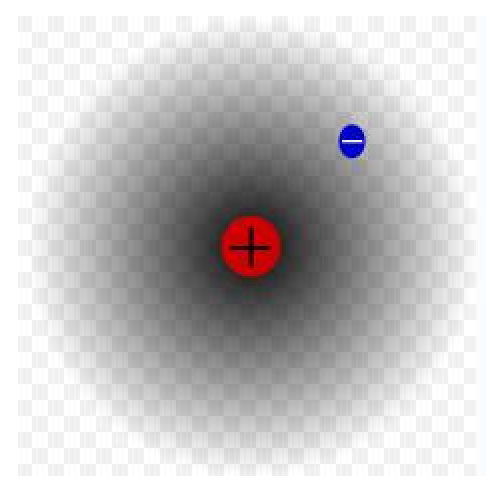
\includegraphics[scale=0.3]{figs/intro1}
\end{figure}

\begin{figure}
\centering
% Source wikipedia
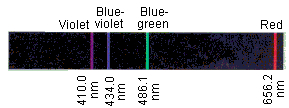
\includegraphics[scale=0.40]{figs/intro2}
\end{figure}

\begin{center}
{\footnotesize Emission spectrum of hydrogen atom}
\end{center}
\end{frame}

\scriptsize

\opage{
\otitle{2.1 \& 2.2 The curvature of the wavefunction \& Qualitative solutions}

\otext
The Schr\"odinger equation can be used to obtain curvature of $\psi$:

$$\frac{d^2\psi}{dx^2} = \frac{2m}{\hbar^2}\left(V - E\right)\psi$$

If $(V - E)\psi < 0$ the curvature goes like $\cap$ or $(V - E)\psi > 0$ then $\cup$. Consider, for example, the following:

\vspace*{0.2cm}

\ofig{harmonic-pot}{0.3}{}

The curvature is large where the amplitude of $\psi$ is large. The solutions must be such that they tend to zero far away from the origin.

}

\opage{
\otitle{2.2 The spectrum of hydrogenlike atoms}

\otext
Eq. (\ref{eq10.10}) can be expressed in \href{http://en.wikipedia.org/wiki/Wavenumber}{\uline{wavenumber}} units (m$^{-1}$; usually cm$^{-1}$ is used):

\aeqn{10.14}{\tilde{E}_n = \frac{E_n}{hc} = \frac{E_n}{2\pi\hbar c} = -\overbrace{\frac{m_ee^4}{4\pi c(4\pi\epsilon_0)^2\hbar^3}}^{\equiv R}
\times\frac{Z^2}{n^2}\textnormal{ ( }\tilde{}\textnormal{ for wavenumber units)}}

\vspace{-1cm}
\begin{columns}
\begin{column}{5.5cm}

\vspace{-0.5cm}
\otext
where $R$ is the \href{http://en.wikipedia.org/wiki/Rydberg_constant}{\uline{Rydberg constant}} and we have assumed that the nucleus has an infinite mass. To be exact, the Rydberg constant depends on the nuclear mass, but this difference is very small. For example, $R_H = 1.096 775 856 \times 10^7$ m$^{-1} = 1.096 775 856 \times 10^5$ cm$^{-1}$, $R_D = 1.097 074 275 \times 10^5$ cm$^{-1}$, and $R_\infty = 1.097 373 153 4 \times 10^5$ cm$^{-1}$. The latter value is for a nucleus with an infinite mass (i.e., $\mu = m_e$).
\end{column}
\hspace*{-1cm}
\begin{column}{5cm}
\ofig{hlines}{0.25}{H atom emission lines}
\end{column}
\end{columns}

}

\opage{
\otext
Eq. (\ref{eq10.14}) can be used to calculate the differences in the energy levels:

\aeqn{10.16}{\Delta\tilde{v}_{n_1,n_2} = \tilde{E}_{n_2} - \tilde{E}_{n_1} = -\frac{R_HZ^2}{n_2^2} + \frac{R_HZ^2}{n_1^2} = R_HZ^2\left(\frac{1}{n_1^2} - \frac{1}{n_2^2}\right)}

\otext
In the previous figure, the \href{http://en.wikipedia.org/wiki/Lyman_series}{\uline{Lyman series}} is obtained with $n_1 = 1$, \href{http://en.wikipedia.org/wiki/Balmer_series}{\uline{Balmer}} with $n_1 = 2$, and \href{http://en.wikipedia.org/wiki/Hydrogen_spectral_series}{\uline{Paschen}} with $n_1 = 3$. The ionization energy (i.e., when the electron is detached from the atom; see previous figure) is given by:

\aeqn{10.18}{E_i = R_HZ^2\left(\frac{1}{1^2} - \frac{1}{\infty}\right)}

For a ground state hydrogen atom (i.e., $n = 1$), the above equation gives a value of 109678 cm$^{-1}$ = 13.6057 eV. Note that the larger the nuclear charge $Z$ is, the larger the binding energy is.

\otext
Recall that the wavefunctions for hydrogenlike atoms are $R_{nl}(r)Y_l^m(\theta,\phi)$ with $l < n$. For the first shell we have only one wavefunction: $R_{10}(r)Y_0^0(\theta,\phi)$. This state is usually labeled as $1s$, where 1 indicates the \href{http://en.wikipedia.org/wiki/Electron_shell}{\uline{shell number}} ($n$) and $s$ corresponds to orbital anular momentum $l$ being zero. For $n = 2$, we have several possibilities: $l = 0$ or $l = 1$. The former is labeled as $2s$. The latter is $2p$ state and consists of three degenerate states: (for example, $2p_x$, $2p_y$, $2p_z$ or $2p_{+1}$, $2p_0$, $2p_{-1}$). In the latter notation the values for $m$ have been indicated as subscripts. Previously, we have seen that:

}

\opage{

\aeqn{10.19}{m = -l, -l+1, ..., 0, ..., l-1, l}

\otext
For historical reasons, the following letters are used to express the value of $l$:

\beqn{10.20}{\phantom{\textnormal{symbo}}l = 0, 1, 2, 3, ...}{\textnormal{symbol} = s, p, d, f, ...}

To summarize the quantum numbers in hydrogenlike atoms:

\aeqn{10.21}{n = 1, 2, 3, ...}
\aeqn{10.22}{l = 0, 2, ..., n-1}
\aeqn{10.23}{m = 0, \pm 1, \pm 2,...,\pm l}

For a given value of $n$, the level is $n^2$ times degenerate. There is one more quantum number that has not been discussed yet: \href{http://en.wikipedia.org/wiki/Spin_quantum_number}{\uline{the spin quantum number}}. For one-electron systems this can have values $\pm\frac{1}{2}$ (will be discussed in more detail later). In absence of magnetic fields the spin levels are degenerate and therefore the total degeneracy of the levels is $2n^2$.

\otext
The total wavefunction for a hydrogenlike atom is ($m$ is usually denoted by $m_l$):

}

\opage{

\aeqn{10.24}{\psi_{n,l,m_l}(r,\theta,\phi) = N_{nl}R_{nl}(r)Y_l^{m_l}(\theta,\phi)}

\beqn{10.25}{N_{nl} = \sqrt{\left(\frac{2Z}{na_0}\right)^3\frac{(n - l - 1)!}{2n\left[(n + l)!\right]}}}
{R_{nl}(r) = \rho^le^{-\rho/2}\underbrace{L_{n-l-1}^{2l+1}(\rho)}_{\begin{matrix}\textsuperscript{associated}\\ \textsuperscript{Laguerre}\\ \textsuperscript{polynomial}\end{matrix}}\textnormal{, }\rho = \frac{2Zr}{na_0}}

\vspace{-0.8cm}
\begin{table}
\begin{tabular}{l@{\extracolsep{1cm}}l@{\extracolsep{1cm}}l@{\extracolsep{1cm}}l}
$n$ & $l$ & $m$ & Wavefunction\\
\hline
1 & 0 & 0 & $\psi_{1s} = \frac{1}{\sqrt{\pi}}\left(\frac{Z}{a_0}\right)^{3/2}e^{-\sigma}$\\
2 & 0 & 0 & $\psi_{2s} = \frac{1}{4\sqrt{2\pi}}\left(\frac{Z}{a_0}\right)^{3/2}(2 - \sigma)e^{-\sigma/2}$\\
2 & 1 & 0 & $\psi_{2p_z} = \frac{1}{4\sqrt{2\pi}}\left(\frac{Z}{a_0}\right)^{3/2}\sigma e^{-\sigma/2}\textnormal{cos}(\theta)$\\
2 & 1 & $\pm 1$ & $\psi_{2p_x} = \frac{1}{4\sqrt{2\pi}}\left(\frac{Z}{a_0}\right)^{3/2}\sigma e^{-\sigma/2}\textnormal{sin}(\theta)\textnormal{cos}(\phi)$\\
  &   &         & $\psi_{2p_y} = \frac{1}{4\sqrt{2\pi}}\left(\frac{Z}{a_0}\right)^{3/2}\sigma e^{-\sigma/2}\textnormal{sin}(\theta)\textnormal{sin}(\phi)$\\
\end{tabular}
\label{table10.2}
\caption{Cartesian hydrogenlike wavefunctions ($\sigma = \frac{Zr}{a_0}$).}
\end{table}

}

\opage{

\begin{table}
% Table continued
\begin{tabular}{l@{\extracolsep{1cm}}l@{\extracolsep{1cm}}l@{\extracolsep{1cm}}l}
$n$ & $l$ & $m$ & Wavefunction\\
\hline
3 & 0 & 0 & $\psi_{3s} = \frac{1}{81\sqrt{3\pi}}\left(\frac{Z}{a_0}\right)^{3/2}\left(27 - 18\sigma + 2\sigma^2\right)e^{-\sigma/3}$\\
3 & 1 & 0 & $\psi_{3p_z} = \frac{\sqrt{2}}{81\sqrt{\pi}}\left(\frac{Z}{a_0}\right)^{3/2}\left(6 - \sigma\right)\sigma e^{-\sigma/3}\textnormal{cos}(\theta)$\\
3 & 1 & $\pm 1$ & $\psi_{3p_x} = \frac{\sqrt{2}}{81\sqrt{\pi}}\left(\frac{Z}{a_0}\right)^{3/2}\left(6 - \sigma\right)\sigma  e^{-\sigma/3}\textnormal{sin}(\theta)\textnormal{cos}(\phi)$\\
  &   &         & $\psi_{3p_y} = \frac{\sqrt{2}}{81\sqrt{\pi}}\left(\frac{Z}{a_0}\right)^{3/2}\left(6 - \sigma\right)\sigma 
e^{-\sigma/3}\textnormal{sin}(\theta)\textnormal{sin}(\phi)$\\
3 & 2 & 0 & $\psi_{3d_{z^2}} = \frac{1}{81\sqrt{6\pi}}\left(\frac{Z}{a_0}\right)^{3/2}\sigma^2e^{-\sigma/3}\left(3\textnormal{cos}^2(\theta) - 1\right)$\\
3 & 2 & $\pm 1$ & $\psi_{3d_{xz}} = \frac{\sqrt{2}}{81\sqrt{\pi}}\left(\frac{Z}{a_0}\right)^{3/2}\sigma^2  e^{-\sigma/3}\textnormal{sin}(\theta)\textnormal{cos}(\theta)\textnormal{cos}(\phi)$\\
  &   &         & $\psi_{3d_{yz}} = \frac{\sqrt{2}}{81\sqrt{\pi}}\left(\frac{Z}{a_0}\right)^{3/2}\sigma^2 
e^{-\sigma/3}\textnormal{sin}(\theta)\textnormal{cos}(\theta)\textnormal{sin}(\phi)$\\

3 & 2 & $\pm 2$ & $\psi_{3d_{x^2-y^2}} = \frac{1}{81\sqrt{3\pi}}\left(\frac{Z}{a_0}\right)^{3/2}\sigma^2  e^{-\sigma/3}\textnormal{sin}^2(\theta)\textnormal{cos}(2\phi)$\\
  &   &         & $\psi_{3d_{xy}} = \frac{1}{81\sqrt{3\pi}}\left(\frac{Z}{a_0}\right)^{3/2}\sigma^2 
e^{-\sigma/3}\textnormal{sin}^2(\theta)\textnormal{sin}(2\phi)$\\

\end{tabular}
\caption{Cartesian hydrogenlike wavefunctions (continued).}
\end{table}

}

\opage{

\ofig{orbitals}{0.3}{Plots demonstrating the shapes of different hydrogenlike atomic orbitals.}

}

\opage{

\begin{table}
\begin{tabular}{l@{\extracolsep{1cm}}l}
$L_0^k(x)$ & $1$\\
$L_1^k(x)$ & $k-x+1$\\
$L_2^k(x)$ & $\frac{1}{2} \left(k^2+3 k+x^2-2 (k+2) x+2\right)$\\
$L_3^k(x)$ & $\frac{1}{6} \left(k^3+6 k^2+11 k-x^3+3 (k+3) x^2-3 (k+2)(k+3) x+6\right)$\\
$L_4^k(x)$ & $\frac{1}{24} (x^4-4 (k+4) x^3+6 (k+3) (k+4) x^2-4 k(k (k+9)+26) x$\\
           & $-96 x+k (k+5) (k (k+5)+10)+24)$\\
\end{tabular}
\caption{Examples of associated Laguerre polynomials.}
\end{table}

\otext
\textbf{Advanced topic.} The following Maxima program generates the associated Laguerre polynomial $L_5^k(x)$:\\

\otext
\verbatiminput{maxima/laguerre.mac}

\vfill

}

\opage{
\otitle{2.3 Eigenfunctions and probability densities for hydrogenlike atoms}

\otext
A wavefunction for a one-electron system is called an orbital. For an atomic system such as H (hydrogen atom), it is called an \href{http://en.wikipedia.org/wiki/Atomic_orbital}{\uline{atomic orbital}}.\\

\otext
The orbital plots on the previous slide demonstrated the shapes of the orbitals but this does not tell us anything about the radial extent (i.e., how far the orbital reaches).
\vspace{-0.7cm}
\begin{columns}
\begin{column}{5cm}
\ofig{radial}{0.25}{Radial wavefunctions $N_{nl}\times R_{nl}(r)$.}
\end{column}
\begin{column}{5cm}
\ofig{radial2}{0.25}{Radial probabilities $P_{nl}(r)$.}
\end{column}
\end{columns}

}

\opage{
\otext
\textbf{Advanced topic.} The following Maxima program can be used to plot the radial wavefunctions on the previous page (if wxMaxima is used, replace plot2d with wxplot2d):\\

\verbatiminput{maxima/radial.mac}

}

\opage{
\otext
Note that:

\begin{itemize}
\item As the value of $Z$ is increased, the radial extent decreases. This indicates that for higher nuclear charge, the electrons will reside closer to the nucleus.
\item The radial functions have $n - l - 1$ zero values (``nodes'') between distances from zero to infinity.
\item The existence of the nodes makes the wavefunctions orthogonal. For example, $\psi_{1s}$ and $\psi_{2s}$ in hydrogenlike atoms are orthogonal.
\end{itemize}

\otext
When visualizing the radial probabilities, it is possible to do directly plot the square of the radial wavefunction ($R_{nl}^2$) or the radial probability density ($P_{nl}$):

\aeqn{10.28}{P_{nl}(r) = r^2N_{nl}^2R_{nl}^2(r)}

According to this expression, the most probable radius for an electron on hydrogen atom $1s$ orbital is $a_0$ (the Bohr radius). Previous figures showed examples of $R_{nl}$ and $P_{nl}$. Probability densities are useful, for example, in understanding charge distributions in atoms and molecules.

}

\opage{
\otext
As the principal quantum number $n$ increases, the electron moves out to greater distances from the nucleus. The average distance for an electron in a given orbital (with quantum numbers $n$ and $l$) is given by (this is \textit{not} the expectation value):

\beqn{10.29}{\langle r\rangle_{nl} = \int_0^\infty r\times P_{nl}(r)dr}{= \frac{n^2a_0}{Z}\lbrace 1 + \frac{1}{2}\lbrack  1 - \frac{l(l+1)}{n^2}\rbrack\rbrace}

Note that the expectation value of $r$ and the most probable value for $r$ are not equal. The expectation value can be thought of like ``an average'' and the most probable value like a ``maximum value''.

\otext
The probability density (including the angular variables) for the electron in a hydrogenlike atom is given by:

\aeqn{10.31}{\psi^*_{nlm}(r,\theta,\phi)\psi_{nlm}(r,\theta,\phi) = |N_{nl}R_{nl}(r)Y_l^m(\theta,\phi)|^2}

This function depends on three variables and is difficult to plot directly. Previously, we have seen that it is convenient to plot contour levels, which contain the electron with, for example, 90\% probability.

}

\opage{
\otext
For degenerate states with $l > 0$, we have an additional degree of freedom in choosing how to represent the orbitals. In fact, any linear combination of given $3l$ orthogonal eigenfunctions corresponding to a degenerate set with orbital angular momentum $l$, is also a solution to the Schr\"odinger equation.

\otext
Two commonly used representations are the Cartesian form, which are real valued functions and have been, in the case of $l = 1$, denoted by $p_x$, $p_y$ and $p_z$, and the eigenfunctions of the angular momentum ($L^2$ and $L_z$), which are complex valued and are denoted by $p_{-1}$, $p_0$ and $p_{+1}$. The relation between the representations is:

\vspace*{-0.3cm}

\ceqn{10.32}{p_x = -\frac{1}{\sqrt{2}}\left( p_{+1} - p_{-1}\right)\propto \textnormal{sin}(\theta)\textnormal{cos}(\phi)\propto x}
{p_y = \frac{i}{\sqrt{2}}\left( p_{+1} + p_{-1}\right)\propto \textnormal{sin}(\theta)\textnormal{sin}(\phi)\propto y}
{p_z = p_0}

Note by combining $p_x$, $p_y$ and $p_z$, the lobe of the orbital can be made to point at any direction. For $d$-orbitals, we have five degenerate levels:

\vspace*{-0.3cm}

\ceqn{10.33}{d_{x^2 - y^2} = \frac{1}{\sqrt{2}} \left(d_{+2} + d_{-2}\right)\textnormal{, }d_{xy} = -\frac{i}{\sqrt{2}}\left( d_{+2} - d_{-2}\right)}
{d_{xz} = -\frac{1}{\sqrt{2}}\left( d_{+1} - d_{-1}\right)\textnormal{, }d_{yz} = \frac{i}{\sqrt{2}}\left( d_{+1} + d_{-1}\right)}
{d_{z^2} = d_0}

}

\opage{
\otitle{2.4 Work of compression and expansion of a gas at constant temperature}

\otext
Work can be done on/by a gas upon compression/expansion. In the following example gas is the system and the surroundings constitutes of a piston and a thermostat (i.e. a container that keeps the temperature constant).

\begin{columns}

\begin{column}{5cm}
Assumptions:
\begin{itemize}
\item No friction
\item No external pressure outside the cylinder (from atmosphere)
\item Cylinder immersed in a thermostat (constant $T$)
\end{itemize}

\end{column}

\begin{column}{5cm}

\ofig{constant-temperature}{0.5}{Compression by a piston with mass $m$.}

\end{column}

\end{columns}

\vspace*{0.2cm}

Consider a \underline{two stage process}:\\
\begin{enumerate}
\item Pressure $P_1$, Volume $V_1$ and Temperature $T$ (stops removed but the piston has not yet fallen down due to gravity).\\
\item Pressure $P_2$, Volume $V_2$ and Temperature $T$ (the piston has fallen down).\\
\end{enumerate}

}

\opage{

\otext
At both points the external pressure is $P_{ext} = \frac{mg}{A}$ where $A$ is the area of the piston. Thus the force pushing the piston down is $mg$. At the end of the process the gas pressure will be the same as the external pressure: $P_{ext} = P_2$. Recall that work was defined as ``force $\times$ distance'', which in this case means (see Eq. (\ref{eq2.4}), $P_1 < P_2$):

\aeqn{2.31}{w_{comp} = \int\limits_{ini}^{fin}\inex{dw} = \int\limits_{ini}^{fin} \umark{-P_{ext}}{\textnormal{constant}}dV = -P_2(V_2 - V_1) = P_2(V_1 - V_2) > 0}

or expressed in another way without reference to $P_2$:

\aeqn{2.31a}{w_{comp} = \int\limits_{ini}^{fin}\umark{-P_{ext}}{\textnormal{constant}}dV = \frac{mg}{A}\times\umark{\left(Ah\right)}{=\Delta V} = mg\times h\textnormal{ (force }\times\textnormal{distance)}}

where the positive sign for $w_{comp}$ signifies that work was done on the system and $h$ denotes the distance that the piston moved (the shaded area on the previous page $P$-$V$ plot).

\hrulefill

Next, consider expansion of a gas in a two stage process:

}

\opage{

\ofig{constant-temperature2}{0.5}{Expansion of gas (piston pushed up).}

\otext
Work done by the system is given by ($P_1 > P_2$, $P_2 = P_{ext}$):

\aeqn{2.33}{w_{exp} = \int\limits_{ini}^{fin}\umark{-P_{ext}}{\textnormal{constant}}dV = -P_{ext}(V_2 - V_1) = P_2(V_1 - V_2) < 0}

\underline{Note:} $\left|w_{comp}\right| > \left|w_{exp}\right|$. More work is required to compress the gas than can be obtained by expansion. This process is \textbf{irreversible}. 

\vspace*{0.4cm}

Is it possible to move the piston in such a way that $\left|w_{exp}\right| = \left|w_{comp}\right|$? In other words, is it possible to make the process \textbf{reversible} in terms of work?

}

\opage{

\otext
\underline{Yes.} Instead of single-step compression, we should use many compression steps with increasing external pressure $P_{ext}$. This can be achieved by increasing the mass gradually ($m_1 < m_2 < m_3 < ...$):

\ofig{reversible}{0.4}{}

In other words: do not apply all the force at once but increase it gradually. \textit{Note that in a reversible process the pressure inside the cylinder and the external pressure are equal at all times.} In this case the work is obtained by ($P$ is the pressure inside the cylinder):

\aeqn{2.32}{w_{comp} = \int\limits_{ini}^{fin}\inex{dw} = -\int\limits_{V_1}^{V_2}P_{ext}dV = -\int\limits_{V_1}^{V_2}PdV}

}

\opage{

\otext
Expansion work $w_{exp}$ can also be carried out using infinite expansion steps ($m_1 > m_2 > m_3 ...$):

\ofig{reversible2}{0.4}{}

This infinite expansion process is also reversible. The expression for work is now:

\aeqn{2.32a}{w_{exp} = \int\limits_{ini}^{fin}\inex{dw} = -\int\limits_{V_2}^{V_1}PdV}

Work over one closed cycle (reversible compression followed by reversible expansion):

\aeqn{2.34}{w_{cycle} = \umark{-\int\limits_{V_1}^{V_2}PdV}{\textnormal{compression}} \umark{-\int\limits_{V_2}^{V_1}PdV}{\textnormal{expansion}} = -\int\limits_{V_1}^{V_2}PdV + \int\limits_{V_1}^{V_2}PdV = 0}

Thus the infinitesimal process is reversible. Many calculations can be carried out exactly only for reversible processes. Most processes in nature are, however, irreversible. Sometimes they can be approximated as reversible processes.

}

\opage{

\otext
For a reversible process $P_{ext} = P$ (in the cylinder) always. Assuming that the gas in the cylinder is ideal, we have for \textit{reversible expansion} ($T$ constant, $V_1 < V_2$, \textit{ini} = 1 and \textit{fin} = 2):

\vspace*{-0.2cm}

\aeqn{2.35}{w_{exp,rev} = -\int\limits_{V_1}^{V_2}P_{ext}dV = -\int\limits_{V_1}^{V_2}PdV = -\int\limits_{V_1}^{V_2}\frac{nRT}{V}dV = -nRT\ln\left(\frac{V_2}{V_1}\right)}

For reversible compression ($T$ constant, $V_1 > V_2$, \textit{ini} = 1 and \textit{fin} = 2), we have $w_{comp,rev} = -nRT\ln\left(\frac{V_2}{V_1}\right) > 0$.

\vspace*{0.2cm}

For an ideal gas at constant temperature, we have $P_1V_1 = P_2V_2$ and Eq. (\ref{eq2.35}) can then be written:

\aeqn{2.36}{w_{exp,rev} = -nRT\ln\left(\frac{V_2}{V_1}\right) = -nRT\ln\left(\frac{P_1}{P_2}\right) = nRT\ln\left(\frac{P_2}{P_1}\right)}

The maximum amount of work of isothermal expansion of a van der Waals gas is:

\vspace*{-0.2cm}

\aeqn{2.37}{w_{exp,rev} = -\int\limits_{V_1}^{V_2}\left(\frac{nRT}{V-nb} - \frac{an^2}{V^2}\right)dV = -nRT\ln\left(\frac{V_2 - nb}{V_1 - nb}\right) + an^2\left(\frac{1}{V_1} - \frac{1}{V_2}\right)}

\vspace*{0.2cm}

\underline{Note:} During reversible processes the system and the surroundings are in equilibrium. However, such processes are ideal since they take infinitely long time to proceed.

}

\opage{

\otext
\textbf{Example.} Calculate the work done when 50 g of iron reacts with hydrochloric acid in (a) a closed vessel of fixed volume, (b) an open beaker at 25 \degree{}C. The reaction is:

$$\textnormal{Fe}(s) + 2\textnormal{HCl}(aq) \rightarrow \textnormal{FeCl}_2(aq) + \textnormal{H}_2(g)$$

Assume that H$_2$ follows the ideal gas law.

\vspace*{0.2cm}

\textbf{Solution.}\\

\vspace*{0.2cm}

(a) The volume cannot change, so no $PV$-work is done and $w_{exp} = 0$.\\
(b) The gas drives back the atmosphere and therefore $w_{exp} = -P_{ext}\Delta V$. We can neglect the initial volume ($V_1$) because the final volume ($V_2$) after production of gas, is much larger. We assume that H$_2$ behaves according to the ideal gas law ($n$ moles of H$_2$):

$$\Delta V = V_2 - V_1 \approx V_2 = \frac{nRT}{P} = \frac{nRT}{P_{ext}}$$

where $P$ is the gas pressure and $P_{ext}$ the atmospheric pressure. Note that solids have negligible volumes compared to gases and therefore we have:

$$w_{exp} = -P_{ext}\Delta V \approx -P_{ext}\times \frac{nRT}{P_{ext}} = -nRT$$

When 1 mol of Fe is consumed in the reaction, 1 mol H$_2$ is produced.

}

\opage{

\otext
Because the molar mass of Fe is 55.85 g mol$^{-1}$, it follows that:

$$w_{exp} \approx -\frac{50\textnormal{ g}}{55.85\textnormal{ g mol}^{-1}}\times \left(8.3145\textnormal{ JK}^{-1}\textnormal{mol}^{-1}\right)\times\left(298.15\textnormal{ K}\right) = -2.2\textnormal{ kJ}$$

Thus the system (H$_2$ gas from the reaction) does 2.2 kJ of work driving back the atmosphere.

\vspace*{0.2cm}

\textbf{Example.} Work of expansion of an ideal gas. One mole of an ideal gas expands from 5 to 1 bar at 298 K. Calculate $w_{exp}$ (a) for reversible expansion and (b) for an irreversible expansion against a constant external pressure of 1 bar.

\vspace*{0.2cm}

\textbf{Solution.} (a) We use Eq. (\ref{eq2.36}) with $P_1 = 5$ bar (\textit{ini}) and $P_2 = 1$ bar (\textit{fin}):

$$w_{exp,rev} = nRT\ln\left(\frac{P_2}{P_1}\right) = \left(1\textnormal{ mol}\right)\times\left(8.3145\textnormal{ J K}^{-1}\textnormal{ mol}^{-1}\right)\times\left(298\textnormal{ K}\right)\times\ln\left(\frac{1\textnormal{ bar}}{5\textnormal{ bar}}\right)$$

\vspace*{-0.4cm}

$$ = -4000\textnormal{ J}$$

\vspace*{-0.4cm}

\phantom{\textbf{Solution. }}(b) The irreversible work is given by Eq. (\ref{eq2.33}):

$$w_{exp,irrev} = -P_2\left(V_2 - V_1\right) = -P_2\left(\frac{nRT}{P_2} - \frac{nRT}{P_1}\right) = nRT\left(\frac{P_2}{P_1} - 1\right)$$
$$\left(1\textnormal{ mol}\right) \times \left(8.3145\textnormal{ J K}^{-1}\textnormal{ mol}^{-1}\right) \times \left(298\textnormal{ K}\right) \times \left(\frac{1\textnormal{ bar}}{5\textnormal{ bar}} - 1\right) = -2000\textnormal{ J}$$

}

\opage{
\otitle{2.5 Electron spin}

\begin{columns}
\hspace*{-2cm}
\begin{column}{5cm}
\begin{columns}
\begin{column}{2cm}
\operson{walter_gerlach}{0.15}{Walter Gerlach (1889 - 1979)}
\end{column}
\hspace*{-0.5cm}
\begin{column}{3cm}
\operson{otto_stern}{0.265}{Otto Stern (1889 - 1979), Nobel price 1943}
\end{column}
\end{columns}
\operson{ukg}{0.15}{\vspace*{0.1cm}
L: George Uhlenbeck (1900 - 1988),\\
M: Hendrik Kramers (1894 - 1952),\\
\vspace*{-0.1cm}
R: Samuel Goudsmit (1902 - 1978).}
\end{column}\hspace*{-1.5cm}\vline
\hspace*{0.5cm}
\begin{column}{4cm}

\otext
\underline{Stern-Gerlach experiment:}\\

\ofig{stern-gerlach-exp}{0.3}{}

\otext
Note that silver atoms have one unpaired electron.\\

\vspace*{0.3cm}
 
The electron appears to have an intrinsic magnetic moment, which originates from electron spin.
\end{column}

\end{columns}

}

\opage{

\otext
The Schr\"odinger equation does not account for electron spin. The concept of electron spin
originates from Dirac's relativistic equation. However, it can be included in the Schr\"odinger
equation as an extra quantum number ($s$). Furthermore, it appears to follow the general laws of angular momentum.

\otext
The spin angular momentum vector $\vec{S}$ has a magnitude: $|\vec{S}| = S = \sqrt{s(s+1)}\hbar$
where $s$ is the spin quantum number ($\frac{1}{2}$). A crude way of thinking about the origin of the spin
angular momentum is to consider the magnetic moment to arise from the internal spinning
motion of the electron about its own axis. However, this is not exactly true because electrons
have internal structure that we have ignored here.

\otext
To summarize the behavior of electron spin angular momentum:

\aeqn{10.44}{S^2 = s(s+1)\hbar^2 = \frac{3}{4}\hbar^2\textnormal{ (since }s = \frac{1}{2}\textnormal{)}}

\aeqn{10.45}{S_z = m_s\hbar\textnormal{ with }m_s = \pm\frac{1}{2}\textnormal{ (}+\frac{1}{2} = \textnormal{``spin up''; }-\frac{1}{2}
= \textnormal{``spin down'')}}

The corresponding operators are denoted by $\hat{S}_z$ and $\hat{S}^2$. How about the eigenfunctions?

\otext
The eigenfunctions are denoted by $\alpha$ and $\beta$ and we don't write down their specific forms.
The following relations apply for these eigenfunctions:

}

\opage{

\otext
\aeqn{10.46}{\hat{S}^2\alpha\equiv \hat{S}^2|\alpha\rangle = \frac{1}{2}\left(\frac{1}{2} + 1\right)\hbar^2\alpha = \frac{3}{4}\hbar^2\alpha\equiv\frac{3}{4}\hbar^2|\alpha\rangle}

\aeqn{10.47}{\hat{S}^2\beta\equiv \hat{S}^2|\beta\rangle = \frac{1}{2}\left(\frac{1}{2} + 1\right)\hbar^2\beta = \frac{3}{4}\hbar^2\beta\equiv\frac{3}{4}\hbar^2|\beta\rangle}

\aeqn{10.48}{\hat{S}_z\alpha\equiv \hat{S}_z|\alpha\rangle = +\frac{1}{2}\hbar\alpha\equiv +\frac{1}{2}\hbar |\alpha\rangle}

\aeqn{10.49}{\hat{S}_z\beta\equiv \hat{S}_z|\beta\rangle = -\frac{1}{2}\hbar\beta\equiv -\frac{1}{2}\hbar |\beta\rangle}

Note that all the following operators commute: $\hat{H}$, $\hat{L}^2$, $\hat{L}_z$, $\hat{S}^2$, and $\hat{S}_z$. This means that they all can be specified simultaneously. The spin eigenfunctions are taken to be orthonormal:

\aeqn{10.50}{\int\alpha^*\alpha d\sigma\equiv\langle\alpha|\alpha\rangle = \int\beta^*\beta d\sigma\equiv\langle\beta|\beta\rangle = 1}

\aeqn{10.51}{\int\alpha^*\beta d\sigma\equiv\langle\alpha|\beta\rangle = \int\beta^*\alpha d\sigma\equiv\langle\beta|\alpha\rangle = 0}

where the integrations are over variables that the spineigen functions depend on.
Note that we have not specified the actual forms these eigenfunctions. We have only
stated that they follow from the rules of angular momentum. A complete wavefunction
for a hydrogen like atom must specify also the spin part. The total wavefunction is then a product of the spatial
wavefunction and the spin part.

}

\opage{

% TODO: Specify how S_x and S_y operate on spin functions.

\otext
Note that analogously, the $\hat{S}_x$ and $\hat{S}_y$ operators can be defined. These do not commute with $\hat{S}_z$.
Because electrons have spin angular momentum, the unpaired electrons in silver atoms (Stern-Gerlach experiment)
produce an overall magnetic moment (``the two two spots of silver atoms''). The spin magnetic moment is proportional to its spin angular momentum (compare with \ref{eq10.36}):

\aeqn{10.52}{\vec{\hat{\mu}}_S = -\frac{g_ee}{2m_e}\vec{\hat{S}}}

where $g_e$ is the free electron $g$-factor (2.002322 from quantum electrodynamics). The $z$-component of the spin magnetic moment is ($z$ is the quantiziation axis):

\aeqn{10.53}{\hat{\mu}_z = -\frac{g_ee}{2m_e}\hat{S}_z}

Since $S_z$ is given by \ref{eq10.45}, we have:

\aeqn{10.54}{\mu_z = -\frac{g_ee\hbar}{2m_e}m_s = -g_e\mu_Bm_s}

Thus the total energy for a spin in an external magnetic field is:

\aeqn{10.55}{E = g_e\mu_Bm_sB}

where $B$ is the magnetic field strength (in Tesla).

}

\opage{

\otext
By combining the contributions from the hydrogenlike atom Hamiltonian and the orbital
and electron Zeeman terms, we have the total Hamiltonian:

\aeqn{10.56}{\hat{H} = \hat{H}_0 + \frac{eB}{2m_e}\hat{L}_z + \frac{g_eeB}{2m_e}\hat{S}_z = \hat{H}_0 + \frac{eB}{2m_e}\left(\hat{L}_z + g_e\hat{S}_z\right)}

The eigenvalues of this operator are (derivation not shown):

\aeqn{10.57}{E_{n,m_l,m_s} = -\frac{m_ee^4Z^2}{2(2\pi\epsilon_0)^2\hbar n^2} + \frac{eB\hbar}{2m_e}\left(m_l + g_em_s\right)}

\ofig{hydrogen_zeeman}{0.5}{Splitting of hydrogenlike atom energy levels in external magnetic field}

}

\opage{
\otitle{2.6 Change in state at constant volume}

\otext
Previously we have kept temperature constant and concentrated on the concept of work. In this section, under constant volume, heat must also be considered (here work $w$ will be zero). The amount of heat ($q$) can be measured by determining the change in temperature of a mass of material that absorbs the heat. The heat capacity ($C$) of the system is defined as:

\vspace*{-0.1cm}

\aeqn{2.44a}{C = \frac{\inex{dq}}{dT}\textnormal{ or }CdT = \inex{dq}}

where the heat capacity acts as a proportionality constant between change in temperature and the amount of heat. Notice that the differential corresponding to heat is \textit{inexact}. This means that a path must be specified along which the differential is evaluated.

\vspace*{0.25cm}

For a chemically inert system we can use two variables for describing the system ($T$ and $V$ chosen here). Because the internal energy $U$ is a state function (i.e. the corresponding differential is exact), we have the total differential of $U$:

\aeqn{2.44}{dU = \left(\frac{\partial U}{\partial T}\right)_VdT + \left(\frac{\partial U}{\partial V}\right)_TdV}

Substituting $dU = dq - P_{ext}dV$ in Eq. (\ref{eq2.44}) gives (only $PV$-work included):

\aeqn{2.45}{\inex{dq} = \left(\frac{\partial U}{\partial T}\right)_VdT + \left[P_{ext} + \left(\frac{\partial U}{\partial V}\right)_T\right]dV}

By choosing the path in such a way that the volume $V$ is constant, we have $dV = 0$ and:

}

\opage{

\otext

\aeqn{2.46}{\inex{dq}_V = \left(\frac{\partial U}{\partial T}\right)_V dT}

Both the temperature and the heat transfer can be measured and thus it is convenient to define heat capacity $C_V(T)$ at constant volume as:

\aeqn{2.47}{C_V(T) \equiv \frac{\inex{dq}_V}{dT} = \left(\frac{\partial U}{\partial T}\right)_V}

For one mole of substance, heat capacity is denoted by $\bar{C}_V$.

\vspace*{0.25cm}

\underline{Note:} Temperature and heat are two different quantities. On molecular scales temperature is related to the kinetic energy distribution of molecules in the substance. Heat is related to the total energy of molecules (including potential energy).

\vspace*{0.3cm}

At constant volume, Eq. (\ref{eq2.47}) may be multiplied by $dT$ and integrated (see also Eq. (\ref{eq2.46})):

\aeqn{2.48}{\Delta U_V = \int\limits_{T_1}^{T_2}C_V(T)dT = q_V}

If $C_V$ is approximately constant between $T_1$ and $T_2$, we can simplify the above result:

\aeqn{2.49}{\Delta U_V \approx C_V\left(T_2 - T_1\right) = C_V\Delta T}

}

\opage{

\otext
Now we know what $\left(\frac{\partial U}{\partial T}\right)_V$ means but how about $\left(\frac{\partial U}{\partial V}\right)_T$? To see this, we keep $T$ constant (Eq. (\ref{eq2.44})):

\vspace*{-0.25cm}

\begin{columns}

\begin{column}{4cm}
\ofig{joule-exp}{0.5}{Joule's experiment: Gas expands\\\hspace*{0.2cm} into vacuum}
\end{column}

\begin{column}{6cm}

\aeqn{2.50}{\inex{dq} = \left[P_{ext} + \left(\frac{\partial U}{\partial V}\right)_T\right]dV}

Joule found in his experiments that $\Delta T\approx 0$ and therefore $q \approx 0$. Rigorously this can be shown to hold for ideal gases. This implies that for ideal gases we have:

\aeqn{2.50b}{\inex{dq} = 0}

\end{column}

\end{columns}

\vspace*{0.3cm}

If we consider an ideal gas in a process where $P_{ext} = 0$ and $dV \ne 0$ (Joule's experiment), it follows that (Eq. (\ref{eq2.50})):

\aeqn{2.50d}{\left(\frac{\partial U}{\partial V}\right)_T = 0\textnormal{ for an ideal gas}}

\underline{This result does not hold for real gases.} In real gases molecules interact with each other and a change in volume affects the average distance between molecules.

}

\opage{
\otitle{2.7 Helium atom}

\otext
The Schr\"odinger equation for helium atom is already extremely complicated from
the mathematical point of view. No analytic solutions to this equation has been found.
However, with certain approximations, useful results can be obtained.
The Hamiltonian for He atom can be written as:

\aeqn{10.61}{\hat{H} = \underbrace{-\frac{\hbar^2}{2m_e}\left(\Delta_1 + \Delta_2\right)}_\textnormal{Kinetic energy} 
\underbrace{- \frac{1}{4\pi\epsilon_0}\left(\frac{Ze^2}{r_1} + \frac{Ze^2}{r_2} \overbrace{- \frac{e^2}{r_{12}}}^\textnormal{Tough!!}\right)}_\textnormal{Potential energy}}

where $\Delta_1$ is the Laplacian for the coordinates of electron 1, $\Delta_2$ for electron 2, $r_1$ is the
distance of electron 1 from the nucleus, $r_2$ is the distance of electron 2 from the nucleus
and $r_{12}$ is the distance between electrons 1 and 2. For He atom $Z = 2$.

\otext
\underline{1. Approximation:} Ignore the ``Tough'' term containing $r_{12}$. In this case the Hamiltonian
consists of a sum of two hydrogenlike atoms:

}

\opage{

\aeqn{10.62}{\hat{H} = \hat{H}_1 + \hat{H}_2}

\aeqn{10.63}{\hat{H}_1 = -\frac{\hbar^2}{2m_e}\Delta_1 - \frac{Ze^2}{4\pi\epsilon_0r_1}}

\aeqn{10.64}{\hat{H}_2 = -\frac{\hbar^2}{2m_e}\Delta_2 - \frac{Ze^2}{4\pi\epsilon_0r_2}}

\otext
Because the Hamiltonian is a sum of two independent parts, the Schr\"odinger equation
separates into two (each hydrogenatom like equation):

\aeqn{10.65}{\hat{H}_1\psi(r_1) = E_1\psi(r_1)}
\aeqn{10.66}{\hat{H}_2\psi(r_2) = E_2\psi(r_2)}

The total energy is a sum of $E_1$ and $E_2$ and the total wavefunction is a product of $\psi(r_1)$ and $\psi(r_2)$. Based on our previous wavefunction table for hydrogenlike atoms, we have:

\aeqn{10.67}{E = E_1 + E_2 \overbrace{=}^\textnormal{(\ref{eq10.41})} -RZ^2\left(\frac{1}{n_1^2} + \frac{1}{n_2^2}\right)}

\aeqn{10.68}{\psi(r_1)\psi(r_2) = \frac{1}{\sqrt{\pi}}\left(\frac{Z}{a_0}\right)^{3/2}e^{-Zr_1/a_0}\frac{1}{\sqrt{\pi}}\left(\frac{Z}{a_0}\right)^{3/2}e^{-Zr_2/a_0}
=\frac{1}{\pi}\left(\frac{Z}{a_0}\right)^3e^{-Z(r_1 + r_2)/a_0}}

}

\opage{

\otext
For a ground state He atom both electron reside on the lowest energy orbital and therefore the total
wavefunction is $\psi(r_1,r_2) = \psi(r_1)\psi(r_2) = \psi(1)\psi(2) = 1s(1)1s(2)$. The energy obtained from this approximation is not sufficiently accurate (missing electron -- electron repulsion) but the wavefunction can be used for qualitative analysis. The variational principle Eq. (\ref{eq10.58}) gives a systematic way to asses how good our approximation is. The exact ground state energy has been found (very extensive analytic \& numerical calculations) as
-79.0 eV. By using the approximate wavefunction, we can calculate the expectation value for energy. This yields -74.8 eV and thus the error in energy for this wavefunction is -5.2 eV. Note that the approximate value is, in accordance with the variational principle, higher than the true energy.

\otext
\underline{2. A better approximation:} We can take the wavefunction from the previous step and use
the nuclear charge $Z$ as a variational parameter. The variational principle states that
minimization of the energy expectation value with respect to $Z$ should approach the true value
from above (but obviously will not reach it). By judging the energy, we can say that this new
wavefunction is better than the previous wavefunction. The obtained value of $Z$ is
less than the true $Z$ (= 2). This can be understood in terms of electrons
shielding the nucleus from each other and hence giving a reduced nuclear charge.
If the wavefunction in Eq. (\ref{eq10.68}) is used in calculating the energy expectation value, we get:

\aeqn{10.70}{E = \langle\psi |\hat{H}|\psi\rangle = ... = \left[ Z^2 - \frac{27Z}{8}\right]\frac{e^2}{4\pi\epsilon_0a_0}}

}

\opage{

\otext
In order to minimize Eq. (\ref{eq10.70}), we should differentiate it with respect to $Z$ and
set it to zero (extremum point; here it is clear that this point is a minimum):

\aeqn{10.71}{\frac{dE}{dZ} = \left(2Z - \frac{27}{8}\right)\frac{e^2}{4\pi\epsilon_0a_0} = 0}

\otext
The above equation gives $Z = 27/16 \approx 1.7$ and $E \approx -77.5$ eV (previous -74.8 eV and
exact -79.0 eV). This result could be improved by adding more terms and variables into
the trial wavefunction. For example, higher hydrogenlike atom orbitals with appropriate variational coefficients would yield a much better result.

\otext
Another type of approximate method is based on \underline{perturbation theory}, which
would typically assume that the electron -- electron repulsion is treated as an additional
(small) perturbation to case 1) above.

% TODO: could we add time-indep. perturbation theory here and a simple application to He atom?

}

\opage{
\otitle{2.8 Wavepackets}

\otext
A \textit{wavepacket} is a special wavefunction representing a particle that is spatially localized. Note that spatial localization necessarily introduces uncertainty in the momentum. As the name implies, wavepackets are constructed from multiple ``waves'', which here refer to a superposition of momentum eigenfunctions (e.g., $e^{ikx}$ and $e^{-ikx}$). Such a wavepacket can be stationary (i.e., it does not move but may broaden as a function of time; \textit{dispersion}) or it can be given momentum so that it can move in a given direction. In this sense, wavepackets move through space in a similar way as classical particles. A wavepacket can be formed as a superposition of functions $\Psi_k(x,t)$:

\aeqn{2.12}{\Psi_k(x,t) = Ae^{ikx}e^{-iE_kt/\hbar}}

The time dependent phase factor is dictated by the time-dependent Schr\"odinger equation. Instead of summing $\Psi_k(x,t)$, we take a continuum of states and integrate over all momenta to form the wavepacket:

\aeqn{2.13}{\Psi(x,t) = \int\limits_{-\infty}^{\infty}g(k)\Psi_k(x,t)dk}

where $g(k)$ is called the \textit{shape function}. Because of the interference between different $\Psi_k(x,t)$, the overall wavepacket appears localized. The time-dependent part in Eq. (\ref{eq2.12}) makes the wavepacket ``walk''.

}

\opage{

\textbf{Example.} Gaussian wavepacket in harmonic potential.

\begin{center}
\movie[externalviewer]{Click here to start the movie}{osc4.mpg}
\end{center}

\vspace*{0.2cm}

\textbf{Example.} Gaussian wavepacket propagation through two slits (``the two slit experiment'').

\begin{center}
\movie[externalviewer]{Click here to start the movie}{twoslit4.mpg}
\end{center}

}

\opage{
\otitle{2.9 Joule-Thomson expansion}

\vspace*{0.25cm}

\begin{columns}

\begin{column}{2cm}
\ofig{joule-thompson}{0.3}{}\\
\otext

\vspace*{-0.4cm}
{\tiny Adiabatic Joule-Thompson with $T_i \ne T_f$ and $P_i > P_f$.}\\

\end{column}

\begin{column}{9cm}

\begin{columns}

\hspace*{0.4cm}
\begin{column}{7cm}

\vspace*{-0.5cm}

\otext

Joule and Thomson (aka Lord Kelvin) observed a change in gas temperature when it was expanded through a throttle. To push one mole of gas through the throttle, two processes must be considered (temperatures remain constants on each side; they might, however, be different):\\

\begin{enumerate}
\item Compression of gas on the left
\item Expansion of gas on the right
\end{enumerate} 

On \textit{compression}, the work is given by $w_c = P_i\Delta \bar{V} = P_i\left(\bar{V}_i - \bar{V}_f\right) = P_i\left(\bar{V}_i - 0\right) = P_i\bar{V}_i$ (positive because work is done on the system (gas)).

\vspace*{0.15cm}

On \textit{expansion}, the work is now $w_e = P_f\Delta \bar{V} = P_f\left(\bar{V}_i - \bar{V}_f\right) = P_f\left(0 - \bar{V}_f\right) = -P_f\bar{V}_f$ (negative because work is done by the system (gas)).

\end{column}

\begin{column}{2cm}
\operson{joule}{0.1}{James Prescott Joule, English physicist (1818 - 1889)}
\end{column}

\end{columns}

\end{column}

\end{columns}

\vspace*{0.3cm}

The total amount of work (for the gas) is then:

\aeqn{2.73}{w = w_c + w_e = P_i\bar{V}_i - P_f\bar{V}_f}

}

\opage{

\otext
The system is thermally insulated, so that $q = 0$ (no heat exchange). Using Eq. (\ref{eq2.8}) we obtain:

\aeqn{2.74}{\Delta\bar{U} = \bar{U}_f - \bar{U}_i = q + w = P_i\bar{V}_i - P_f\bar{V}_f}

Rearrangement of this equation gives:

\aeqn{2.75}{\umark{\bar{U}_f + P_f\bar{V}_f}{= H_f} = \umark{\bar{U}_i + P_i\bar{V}_i}{= H_i}}

This states that the enthalpy is conserved in the process (\textit{isenthalpic process}). Based on the experimental observation, we define the Joule-Thomson coefficient:

\aeqn{2.77}{\mu_{JT} = \lim\limits_{\Delta P\rightarrow 0}\frac{T_2 - T_1}{P_2 - P_1} = \left(\frac{\partial T}{\partial P}\right)_H}

which gives the change in temperature when pressure changes. At high temperatures the coefficient is negative (J-T process results in heating) and at low temperatures it is positive (J-T process results in cooling). The temperature, where the coefficient is zero, is called the \textit{inversion temperature}. The inversion temperature for N$_2$ is 607 K and for H$_2$ 204 K.\\

\vspace*{0.25cm}

\underline{Notes:}\\

\begin{itemize}
\item The J-T coefficient is zero for ideal gases: $0 = \left(\frac{\partial H}{\partial P}\right)_H = \frac{5}{2}nR\left(\frac{\partial T}{\partial P}\right)_H$.
\item The cooling effect can be understood by decrease in the van der Waals interaction due to lower pressure (i.e. increased potential energy) and decrease in the kinetic energy (i.e. lower temperature).
\end{itemize}

}

\opage{
\otitle{2.10 The periodic table and the aufbau principle}

\otext
The quantum theory of atoms provides an explanation of the structure of the periodic table. The electron subshells in atoms are designated as $1s$, $2s$, $2p$, $3s$, ..., where the number denotes the quantum number $n$ and the letter gives the orbital angular momentum quantum number $l$. According to the Pauli exclusion principle, all $s$ subshells may contain 2 electrons (with $\alpha$ and $\beta$ spins), $p$ subshells 6, and $d$ subshells 10. Thus each subshell may have a maximum of $2(2l + 1)$ electrons.

\otext
To find the ground-state electron configuration of an atom, we add electrons to the subshells (i.e., orbitals) beginning with the lowest energy orbital and remember that two electrons (with opposite
spins) go on each orbital. Note that this approach is approximate since it relies on the one-electron hydrogenlike atom orbitals. For this reason, it is often difficult to predict the energy order of orbitals. The symbols He, Ne, Ar, ... (or sometimes in brackets) are used to represent closed-shell electron configurations. With this notation it is not necessary to explicitly list the inner shell electron configuration.

\otext
Quantum mechanics explains the logic behind the periodic table of elements: along the columns the number of outer shell electrons varies and along the rows the number of inner shell orbitals increases.

}

\opage{

\ofig{periodic}{0.4}{The periodic table of elements.}

\begin{itemize}
\item Within a row in the periodic table, the atomic radius tends to decrease with the atomic number.
\item Within a column in the table, the atomic radius tends to increase with the atomic number.
\end{itemize}

}

\newcommand{\tsub}[1]{$_\textnormal{\varfont{phv}{1}{#1}}$}
\newcommand{\tsup}[1]{$^\textnormal{\varfont{phv}{1}{#1}}$}
\opage{

% TODO: Complete the table (missing values)
\varfont{phv}{0.5}{
\begin{table}
\begin{tabular}{llllllllll}
Element & Symbol & Atomic & Relative & Atom   & Electron & Term   & Ionization & Electron & Electron\\
        &        & number & atomic   & radius & config.  & symbol & energy     & affinity & negativity\\
        &        &        & mass     & (pm)   &          &        & (eV)       & (eV)     & \\
        &        &        & (AMU)    &        &          &        & I / II     &          & \\
\hline
Actinium    & Ac & 89  & (227)    & 245 & Rn 6d\tsup{1} 7s\tsup{2}                         & \tsup{2}D\tsub{3/2}  & 6.9 / 12.1  & --  & 1.1\\
Aluminum    & Al & 13  & 26.98154 & 202 & Ne 3s\tsup{2} 3p\tsup{1}                         & \tsup{2}P\tsub{1/2}  & 6.0 / 18.8  & 0.5 & 1.5\\
Americium   & Am & 95  & (243)    & 242 & Rn 5f\tsup{7} 7s\tsup{2}                         & \tsup{8}S\tsub{7/2}  & -- / --     & --  & 1.3\\
Antimony    & Sb & 51  & 121.75   & 168 & Kr 4d\tsup{10} 5s\tsup{2} 5p\tsup{3}             & \tsup{4}S\tsub{3/2}  & 8.6 / 16.5  & --  & 1.9\\
Argon       & Ar & 18  & 39.948   & 89  & Ne 3s\tsup{2} 3p\tsup{6}                         & \tsup{1}S\tsub{0}    & 15.8 / 27.6 & --  & --\\
Arsenic     & As & 33  & 74.9216  & 141 & Ar 3d\tsup{10} 4s\tsup{2} 4p\tsup{3}             & \tsup{4}S\tsub{3/2}  & 9.8 / 18.6  & --  & 2.0\\
Astatine    & At & 85  & (210)    & 132 & Xe 4f\tsup{14} 5d\tsup{10} 6s\tsup{2} 6p\tsup{5} & \tsup{2}P\tsub{3/2}  & -- / --     & --  & 2.2\\
Barium      & Ba & 56  & 137.327  & 248 & Xe 6s\tsup{2}                                    & \tsup{1}S\tsub{0}    & 5.2 / 10.0  & --  & 0.9\\
Berkelium   & Bk & 97  & (247)    & 226 & Rn 5f\tsup{9} 7s\tsup{2}                         & \tsup{8}H\tsub{17/2} & -- / --     & --  & --\\
Beryllium   & Be & 4   & 9.0122   & 149 & 1s\tsup{2} 2s\tsup{2}                            & \tsup{1}S\tsub{0}    & 9.3 / 18.2  & --  & 1.5\\
Bishmuth    & Bi & 83  & 208.980  & 188 & Xe 4f\tsup{14} 5d\tsup{10} 6s\tsup{2} 6p\tsup{3} & \tsup{4}S\tsub{3/2}  & 7.3 / 16.7  & --  & 1.9\\
Boron       & B  & 5   & 10.811   & 134 & 1s\tsup{2} 2s\tsup{2} 2p\tsup{1}                 & \tsup{2}P\tsub{1/2}  & 8.3 / 25.1  & 0.3 & 2.0\\
Bromine     & Br & 35  & 79.904   & 114 & Ar 3d\tsup{10} 4s\tsup{2} 4p\tsup{5}             & \tsup{2}P\tsub{3/2}  & 11.8 / 21.6 & 3.4 & 2.8\\
Cadmium     & Cd & 48  & 112.412  & 152 & Kr 4d\tsup{10} 5s\tsup{2}                        & \tsup{1}S\tsub{0}    & 9.0 / 16.9  & --  & 1.7\\
Calcium     & Ca & 20  & 40.078   & 225 & Ar 4s\tsup{2}                                    & \tsup{1}S\tsub{0}    & 6.1 / 11.9  & --  & 1.0\\
Californium & Cf & 98  & (251)    & 224 & Rn 5f\tsup{10} 7s\tsup{2}                        & \tsup{5}I\tsub{8}    & -- / --     & --  & --\\
Carbon      & C  & 6   & 12.01115 & 100 & 1s\tsup{2} 2s\tsup{2} 2p\tsup{2}                 & \tsup{3}P\tsub{0}    & 11.3 / 24.4 & 1.2 & 2.5\\
Cerium      & Ce & 58  & 140.12   & 241 & Xe 4f\tsup{1} 5d\tsup{1} 6s\tsup{2}              & \tsup{1}G\tsub{4}    & 6.6 / 12.3  & --  & 1.1\\
Cesium      & Cs & 55  & 132.9054 & 322 & Xe 6s\tsup{1}                                    & \tsup{2}S\tsub{1/2}  & 3.9 / 25.1  & --  & 0.7\\
Chlorine    & Cl & 17  & 35.4527  & 90  & Ne 3s\tsup{2} 3p\tsup{5}                         & \tsup{2}P\tsub{3/2}  & 13.0 / 23.8 & 3.7 & 3.0\\ 
Chromium    & Cr & 24  & 51.9961  & 197 & Ar 3d\tsup{5} 4s\tsup{1}                         & \tsup{7}S\tsub{3}    & 6.8 / 16.5  & --  & 1.6\\
Cobalt      & Co & 27  & 58.9332  & 162 & Ar 3d\tsup{7} 4s\tsup{2}                         & \tsup{4}F\tsub{9/2}  & 7.9 / 17.1  & --  & 1.8\\
Copper      & Cu & 29  & 63.546   & 163 & Ar 3d\tsup{10} 4s\tsup{1}                        & \tsup{2}S\tsub{1/2}  & 7.7 / 20.3  & 2.4 & 1.9\\
Curium      & Cm & 96  & (247)    & 228 & Rn 5f\tsup{7} 6d\tsup{1} 7s\tsup{2}              & \tsup{8}S\tsub{7/2}  & -- / --     & --  & --\\
Dysprosium  & Dy & 66  & 162.50   & 236 & Xe 4f\tsup{10} 6s\tsup{2}                        & \tsup{5}I\tsub{8}    & 6.8 / --    & --  & --\\
Einsteinium & Es & 99  & (252)    & 222 & Rn 5f\tsup{11} 7s\tsup{2}                        & \tsup{5}I\tsub{15/2} & -- / --     & --  & --\\
Erbium      & Er & 68  & 167.26   & 230 & Xe 4f\tsup{12} 6s\tsup{2}                        & \tsup{3}H\tsub{6}    & 6.1 / --    & --  & 1.2\\
Europium    & Eu & 63  & 151.96   & 245 & Xe 4f\tsup{7} 6s\tsup{2}                         & \tsup{8}S\tsub{7/2}  & 5.7 / 11.2  & --  & --\\
Fermium     & Fm & 100 & (257)    & 221 & Rn 5f\tsup{12} 7s\tsup{2}                        & \tsup{3}H\tsub{6}    & -- / --     & --  & --\\
Fluorine    & F  & 9   & 18.998403& 60  & 1s\tsup{2} 2s\tsup{2} 2p\tsup{5}                 & \tsup{2}P\tsub{3/2}  & 17.4 / 35.0 & 3.5 & 4.0\\
Francium    & Fr & 87  & (223)    & 313 & Rn 7s\tsup{1}                                    & \tsup{2}S\tsub{1/2}  & 4.0 / --    & --  & 0.7\\
Gadolinium  & Gd & 64  & 157.25   & 226 & Xe 4f\tsup{7} 5d\tsup{1} 6s\tsup{2}              & \tsup{9}D\tsub{2}    & 6.2 / 12    & --  & 1.1\\
Gallium     & Ga & 31  & 69.723   & 196 & Ar 3d\tsup{10} 4s\tsup{2} 4p\tsup{1}             & \tsup{2}P\tsub{1/2}  & 6.0 / 20.6  & --  & 1.6\\
Germanium   & Ge & 32  & 72.59    & 160 & Ar 3d\tsup{10} 4s\tsup{2} 4p\tsup{2}             & \tsup{3}P\tsub{0}    & 7.9 / 15.9  & --  & 1.8\\
\end{tabular}
\label{table10.3a}
\caption{Atomic data (part 1).}
\end{table}
}

}

\opage{

\varfont{phv}{0.5}{
\begin{table}
\begin{tabular}{llllllllll}
Element & Symbol & Atomic & Relative & Atom   & Electron & Term   & Ionization & Electron & Electron\\
        &        & number & atomic   & radius & config.  & symbol & energy     & affinity & negativity\\
        &        &        & mass     & (pm)   &          &        & (eV)       & (eV)     & \\
        &        &        &          &        &          &        & I / II     &          & \\
\hline
Gold        & Au & 79  & 196.9665 & 162 & Xe 4f\tsup{14} 5d\tsup{10} 6s\tsup{1}            & \tsup{2}S\tsub{1/2}  & 9.2 / 25.1  & --  & 2.4\\
Hafnium     & Hf & 72  & 178.49   & 191 & Xe 4f\tsup{14} 5d\tsup{2} 6s\tsup{2}             & \tsup{3}F\tsub{2}    & 7.0 / 14.9  & --  & 1.3\\
Helium      & He & 2   & 4.002602 & 54  & 1s\tsup{2}                                       & \tsup{1}S\tsub{0}    & 24.6 / 54.4 & 0.2 & --\\
Holmium     & Ho & 67  & 164.930  & 233 & Xe 4f\tsup{11} 6s\tsup{2}                        & \tsup{4}I\tsub{15/2} & -- / --     & --  & 1.2\\
Hydrogen    & H  & 1   & 1.00798  & 79  & 1s\tsup{1}                                       & \tsup{2}S\tsub{1/2}  & 13 / --     & 0.8 & 2.1\\ 
Indium      & In & 49  & 114.82   & 216 & Kr 4d\tsup{10} 5s\tsup{2} 5p\tsup{1}             & \tsup{2}P\tsub{1/2}  & 5.8 / 18.9  & --  & 1.7\\
Iodine      & I  & 53  & 126.9044 & 138 & Kr 4d\tsup{10} 5s\tsup{2} 5p\tsup{5}             & \tsup{2}P\tsub{3/2}  & 10.5 / 19.1 & 3.1 & 2.5\\
Iridium     & Ir & 77  & 192.22   & 165 & Xe 4f\tsup{14} 5d\tsup{7} 6s\tsup{2}             & \tsup{4}F\tsub{9/2}  & 9.2 / --    & --  & 2.2\\
Iron        & Fe & 26  & 55.844   & 168 & Ar 3d\tsup{6} 4s\tsup{2}                         & \tsup{5}D\tsub{4}    & 7.9 / 16.2  & --  & 1.8\\
Kyrpton     & Kr & 36  & 83.80    & 103 & Ar 3d\tsup{10} 4s\tsup{2} 4p\tsup{6}             & \tsup{1}S\tsub{0}    & 14.0 / 24.6 & --  & --\\
Lanthanum   & La & 57  & 138.91   & 232 & Xe 5d\tsup{1} 6s\tsup{2}                         & \tsup{2}D\tsub{3/2}  & 5.6 / 11.4  & --  & 1.1\\
Lawrencium  & Lr & 103 & (261)    & 216 & Rn 5f\tsup{14} 6d\tsup{1} 7s\tsup{2}             & \tsup{2}P\tsub{1/2}  & -- / --     & --  & --\\
Lead        & Pb & 82  & 207.19   & 169 & Xe 4f\tsup{14} 5d\tsup{10} 6s\tsup{2} 6p\tsup{2} & \tsup{3}P\tsub{0}    & 7.4 / 15.0  & --  & 1.8\\
Lithium     & Li & 3   & 6.941    & 205 & 1s\tsup{2} 2s\tsup{1}                            & \tsup{2}S\tsub{1/2}  & 5.4 / 75.6  & 0.6 & 1.0\\
Lutetium    & Lu & 71  & 174.97   & 200 & Xe 4f\tsup{14} 5d\tsup{1} 6s\tsup{2}             & \tsup{2}D\tsub{3/2}  & 6.2 / 14.7  & --  & 1.2\\ 
Magnesium   & Mg & 12  & 24.3051  & 178 & Ne 3s\tsup{2}                                    & \tsup{1}S\tsub{0}    & 7.6 / 15.0  & --  & 1.2\\
Mendelevium & Md & 101 & (258)    & 219 & Rn 5f\tsup{13} 7s\tsup{2}                        & \tsup{2}F\tsub{7/2}  & -- / --     & --  & --\\
Mercury     & Hg & 80  & 200.59   & 156 & Xe 4f\tsup{14} 5d\tsup{10} 6s\tsup{2}            & \tsup{1}S\tsub{0}    & 10.4 / 18.8 & 1.5 & 1.9\\
Molybdenum  & Mo & 42  & 95.93    & 194 & Kr 4d\tsup{5} 5s\tsup{1}                         & \tsup{7}S\tsub{3}    & 7.1 / 16.2  & --  & 1.8\\
Neodymium   & Nd & 60  & 144.24   & 255 & Xe 4f\tsup{4} 6s\tsup{2}                         & \tsup{5}I\tsub{4}    & 6.3 / --    & --  & --\\
Neon        & Ne & 10  & 20.180   & 53  & 1s\tsup{2} 2s\tsup{2} 2p\tsup{6}                 & \tsup{1}S\tsub{0}    & 21.6 / 41.1 & --  & --\\
Neptunium   & Np & 93  & (237)    & 234 & Rn 5f\tsup{4} 6d\tsup{1} 7s\tsup{2}              & \tsup{4}L\tsub{11/2} & -- / --     & --  & 1.3\\
Nickel      & Ni & 28  & 58.69    & 157 & Ar 3d\tsup{8} 4s\tsup{2}                         & \tsup{3}F\tsub{4}    & 7.6 / 18.2  & --  & 1.8\\
Niobium     & Nb & 41  & 92.906   & 100 & Kr 4d\tsup{4} 5s\tsup{1}                         & \tsup{6}D\tsub{1/2}  & 6.9 / 14.3  & --  & 1.6\\
Nitrogen    & N  & 7   & 14.00672 & 81  & 1s\tsup{2} 2s\tsup{2} 2p\tsup{3}                 & \tsup{4}S\tsub{3/2}  & 14.5 / 29.6 & 0.05 & 3.0\\
Nobelium    & No & 102 & (259)    & 218 & Rn 5f\tsup{14} 7s\tsup{2}                        & \tsup{1}S\tsub{0}    & -- / --     & --  & --\\
Osmium      & Os & 76  & 190.2    & 169 & Xe 4f\tsup{14} 5d\tsup{6} 6s\tsup{2}             & \tsup{5}D\tsub{4}    & 8.7 / 17    & --  & 2.2\\
Oxygen      & O  & 8   & 15.9994  & 70  & 1s\tsup{2} 2s\tsup{2} 2p\tsup{4}                 & \tsup{3}P\tsub{2}    & 13.6 / 35.1 & 1.5 & 3.5\\
Palladium   & Pd & 46  & 106.42   & 76  & Kr 4d\tsup{10}                                   & \tsup{1}S\tsub{0}    & 8.3 / 19.4  & --  & 2.2\\
Phosphorus  & P  & 15  & 30.97376 & 130 & Ne 3s\tsup{2} 3p\tsup{3}                         & \tsup{4}S\tsub{3/2}  & 11.0 / 19.7 & 1.1 & 2.1\\
Platinum    & Pt & 78  & 195.08   & 175 & Xe 4f\tsup{14} 5d\tsup{9} 6s\tsup{1}             & \tsup{3}D\tsub{3}    & 9.0 / 18.6  & --  & 2.2\\
Plutonium   & Pu & 94  & (244)    & 244 & Rn 5f\tsup{6} 7s\tsup{2}                         & \tsup{3}F\tsub{0}    & 5.8 / --    & --  & --\\
Polonium    & Po & 84  & (209)    & 170 & Xe 4f\tsup{14} 5d\tsup{10} 6s\tsup{2} 6p\tsup{4} & \tsup{3}P\tsub{2}    & 8.4 / --    & --  & --\\
Potassium   & K  & 19  & 39.0983  & 280 & Ar 4s\tsup{1}                                    & \tsup{2}S\tsub{1/2}  & 4.3 / 31.8  & 0.8 & 0.8\\
\end{tabular}
\label{table10.3b}
\caption{Atomic data (part 2).}
\end{table}
}

}

\opage{

\varfont{phv}{0.5}{
\begin{table}
\begin{tabular}{llllllllll}
Element & Symbol & Atomic & Relative & Atom   & Electron & Term   & Ionization & Electron & Electron\\
        &        & number & atomic   & radius & config.  & symbol & energy     & affinity & negativity\\
        &        &        & mass     & (pm)   &          &        & (eV)       & (eV)     & \\
        &        &        &          &        &          &        & I / II     &          & \\
\hline
Praseodymium& Pr & 59  & 140.9076 & 258 & Xe 4f\tsup{3} 6s\tsup{2}                         & \tsup{4}I\tsub{9/2}  & 5.8 / --    & --  & 1.1\\
Prometium   & Pm & 61  & (145)    & 251 & Xe 4f\tsup{5} 6s\tsup{2}                         & \tsup{6}H\tsub{5/2}  & -- / --     & --  & --\\
Protactinium& Pa & 91  & (231)    & 239 & Rn 5f\tsup{2} 6d\tsup{1} 7s\tsup{2}              & \tsup{4}K\tsub{11/2} & -- / --     & --  & 1.5\\
Radium      & Ra & 88  & (226)    & 262 & Rn 7s\tsup{2}                                    & \tsup{1}S\tsub{0}    & 5.3 / 10.1  & --  & 0.9\\
Radon       & Rn & 86  & (222)    & 124 & Xe 4f\tsup{14} 5d\tsup{10} 6s\tsup{2} 6p\tsup{6} & \tsup{1}S\tsub{0}    & 10.7 / --   & --  & --\\
Rhenium     & Re & 75  & 186.207  & 173 & Xe 4f\tsup{14} 5d\tsup{5} 6s\tsup{2}             & \tsup{6}S\tsub{5/2}  & 7.9 / 16.6  & --  & 1.9\\
Rhodium     & Rh & 45  & 102.9055 & 179 & Kr 4d\tsup{8} 5s\tsup{1}                         & \tsup{4}F\tsub{9/2}  & 7.5 / 18.1  & --  & 2.2\\
Rubidium    & Rb & 37  & 85.4678  & 268 & Kr 5s\tsup{1}                                    & \tsup{2}S\tsub{1/2}  & 4.2 / 27.5  & --  & 0.8\\
Ruthenium   & Ru & 44  & 101.07   & 183 & Kr 4d\tsup{7} 5s\tsup{1}                         & \tsup{5}F\tsub{5}    & 7.4 / 16.8  & --  & 2.2\\
Samarium    & Sm & 62  & 150.36   & 248 & Xe 4f\tsup{6} 6s\tsup{2}                         & \tsup{7}F\tsub{0}    & 5.6 / 11.2  & --  & 1.2\\
Scandium    & Sc & 21  & 44.95591 & 212 & Ar 3d\tsup{1} 4s\tsup{2}                         & \tsup{2}D\tsub{3/2}  & 6.6 / 12.8  & --  & 1.3\\
Selenium    & Se & 34  & 78.96    & 126 & Ar 3d\tsup{10} 4s\tsup{2} 4p\tsup{4}             & \tsup{3}P\tsub{2}    & 9.8 / 21.5  & 1.7 & 2.4\\
Silicon     & Si & 14  & 28.0855  & 157 & Ne 3s\tsup{2} 3p\tsup{2}                         & \tsup{3}P\tsub{0}    & 8.1 / 16.3  & --  & 1.8\\
Silver      & Ag & 47  & 107.868  & 172 & Kr 4d\tsup{10} 5s\tsup{1}                        & \tsup{2}S\tsub{1/2}  & 7.6 / 21.5  & 2.5 & 1.9\\
Sodium      & Na & 11  & 22.989767& 221 & Ne 3s\tsup{1}                                    & \tsup{2}S\tsub{1/2}  & 5.1 / 47.3  & 0.8 & 0.9\\
Strontium   & Sr & 38  & 87.62    & 220 & Kr 5s\tsup{2}                                    & \tsup{1}S\tsub{0}    & 5.7 / 11.0  & --  & 1.0\\
Sulphur     & S  & 16  & 32.064   & 101 & Ne 3s\tsup{2} 3p\tsup{4}                         & \tsup{3}P\tsub{2}    & 10.4 / 23.4 & 2.1 & 2.5\\
Tantalum    & Ta & 73  & 180.948  & 184 & Xe 4f\tsup{14} 5d\tsup{3} 6s\tsup{2}             & \tsup{4}F\tsub{3/2}  & 7.9 / 16.2  & --  & 1.5\\
Thallium    & Tl & 81  & 204.383  & 205 & Xe 4f\tsup{14} 5d\tsup{10} 6s\tsup{2} 6p\tsup{1} & \tsup{2}P\tsub{1/2}  & 6.1 / 20.4  & --  & 1.8\\
Technetium  & Tc & 43  & (98)     & 172 & Kr 4d\tsup{5} 5s\tsup{2}                         & \tsup{6}S\tsub{5/2}  & 7.3 / 15.3  & --  & 1.9\\
Tellurium   & Te & 52  & 127.60   & 157 & Kr 4d\tsup{10} 5s\tsup{2} 5p\tsup{4}             & \tsup{3}P\tsub{2}    & 9.0 / 18.6  & 3.6 & 2.1\\
Terbium     & Tb & 65  & 158.9253 & 224 & Xe 4f\tsup{9} 6s\tsup{2}                         & \tsup{6}H\tsub{15/2} & 6.7 / --    & --  & 1.2\\
Thorium     & Th & 90  & 232.0381 & 233 & Rn 6d\tsup{2} 7s\tsup{2}                         & \tsup{3}F\tsub{2}    & 7.0 / 11.5  & --  & 1.3\\
Thulium     & Tm & 69  & 168.9342 & 227 & Xe 4f\tsup{13} 6s\tsup{2}                        & \tsup{2}F\tsub{7/2}  & 6.8 / 12.1  & --  & 1.2\\
Tin         & Sn & 50  & 118.710  & 161 & Kr 4d\tsup{10} 5s\tsup{2} 5p\tsup{2}             & \tsup{3}P\tsub{0}    & 7.3 / 14.6  & --  & 1.8\\
Titanium    & Ti & 22  & 47.88    & 197 & Ar 3d\tsup{2} 4s\tsup{2}                         & \tsup{3}F\tsub{2}    & 6.8 / 13.6  & --  & 1.5\\
Tungsten    & W  & 74  & 183.85   & 178 & Xe 4f\tsup{14} 5d\tsup{4} 6s\tsup{2}             & \tsup{4}D\tsub{0}    & 8.0 / 17.7  & --  & 1.7\\
Uranium     & U  & 92  & 238.0289 & 234 & Rn 5f\tsup{3} 6d\tsup{1} 7s\tsup{2}              & \tsup{5}L\tsub{4}    & 6.1 / --    & --  & 1.7\\
Vanadium    & V  & 23  & 50.9415  & 188 & Ar 3d\tsup{3} 4s\tsup{2}                         & \tsup{4}F\tsub{3/2}  & 6.7 / 14.7  & --  & 1.6\\
Xenon       & Xe & 54  & 131.29   & 127 & Kr 4d\tsup{10} 5s\tsup{2} 5p\tsup{6}             & \tsup{1}S\tsub{0}    & 12.1 / 21.2 & --  & --\\
Ytterbium   & Yb & 70  & 173.03   & 215 & Xe 4f\tsup{14} 6s\tsup{2}                        & \tsup{1}S\tsub{0}    & 6.3 / 12.1  & --  & 1.1\\
Yttrium     & Y  & 39  & 88.9058  & 204 & Kr 4d\tsup{1} 5s\tsup{2}                         & \tsup{2}D\tsub{3/2}  & 6.4 / 12.2  & --  & 1.3\\
Zinc        & Zn & 30  & 65.40    & 148 & Ar 3d\tsup{10} 4s\tsup{2}                        & \tsup{1}S\tsub{0}    & 9.4 / 18.0  & --  & 1.6\\
Zirconium   & Zr & 40  & 91.224   & 193 & Kr 4d\tsup{2} 5d\tsup{2}                         & \tsup{3}F\tsub{2}    & 6.8 / 13.1  & --  & 1.4\\
\end{tabular}
\label{table10.3c}
\caption{Atomic data (part 3).}
\end{table}
}

}

\opage{

\ofig{aufbau}{0.4}{Demonstration of the aufbau principle.}

}

\opage{
\otitle{2.11 Ionization energy and electron affinity}

\otext
\underline{Ionization energy:} The energy required to remove an electron completely from an atom in the gas phase.\\

\otext
The \underline{first ionization energy} $E_1$ corresponds to: $\textnormal{A} + E_1 \rightarrow \textnormal{A}^+ + e^-$.\\

\otext
The \underline{second ionization energy} $E_2$ corresponds to: $\textnormal{A}^+ + E_2 \rightarrow \textnormal{A}^{2+} + e^-$.\\

\otext
Ionization energies can be determined by irradiating atoms with short wavelength light. Ionization energies of atoms can be found from the previous table of atomic data. As an example, ionization energies of some atoms are given below:

\begin{table}
\begin{tabular}{llllllll}
Element & First & Second & Third & Fourth & Fifth  & Sixth  & Seventh\\
Na      & 496   & 4,560\\
Mg      & 738   & 1,450  & 7,730\\
Al      & 577   & 1,816  & 2,881 & 11,600\\
Si      & 786   & 1,577  & 3,228 & 4,354  & 16,100\\
P       & 1,060 & 1,890  & 2,905 & 4,950  & 6,270  & 21,200\\
S       & 999.6 & 2,260  & 3,375 & 4,565  & 6,950  & 8,490  & 27,107\\
Cl      & 1,256 & 2,295  & 3,850 & 5,160  & 6,560  & 9,360  & 11,000\\
Ar 	& 1,520 & 2,665  & 3,945 & 5,770  & 7,230  & 8,780  & 12,000\\
\end{tabular}
\label{table10.3d}
\caption{Ionization energies of selected atoms (kJ mol$^{-1}$).}
\end{table}

}

\opage{

\otext
\underline{Electron affinity:} This is the energy released in the process of adding an electron to the atom (or molecule). It is usually denoted by $E_a$.

\otext
An example of such process is: Cl(g) + $e^- \rightarrow$ Cl$^-$(g).

\otext
Electron affinities of atoms are listed in the previous table. Note that a negative value means that the energy is lowered when the atom accepts an electron and a positive value means that the energy is increased. In practice, the more negative the value is, the more eager the atom is to accept an electron.

\otext
\underline{Note:} The Koopmans' theorem states that the first ionization energy of an atom or a molecule can be approximated by the energy of the highest occupied orbital (from the Hartree-Fock method). This allows for a simple estimation of the ionization energy by using computational methods.

}

\opage{
\otitle{2.12 Angular momentum of many-electron atoms}

\otext
In many-electron atoms, each electron has both orbital and spin angular momenta. First, for simplicity, consider only the \textit{total} orbital angular momentum operator:

\aeqn{10.96}{\hat{L} = \sum\limits_{i=1}^{N} \hat{l}_i}

where $N$ is the number of electrons and $\hat{l}_i$ is the angular momentum operator for electron $i$. The projection operator along the $z$-axis is then given by:

\aeqn{10.97}{\hat{L}_z = \sum\limits_{i=1}^{N} \hat{l}_{z,i}}

\begin{columns}
\begin{column}{6cm}
By combining this with Eq. (\ref{eq10.35}), we get:

\aeqn{10.98}{M_L = \sum\limits_{i=1}^{N}m_i}

Vector model for adding 3 angular momenta:\\

$\vec{L}$ = Total orbital angular momentum.\\
$\vec{l}_1, \vec{l}_2, \vec{l}_3$ = individual angular momenta.\\

\end{column}
\begin{column}{4cm}
\vspace*{-0.7cm}
\ofig{vector_model}{0.3}{}
\end{column}
\end{columns}

\underline{Notes:} 
\begin{itemize}
\item $\hat{L}, \hat{l}_i$ are operators; $L, l_i$ are the corresponding quantum numbers.
\item We assume a light atom and thus neglect the spin-orbit coupling.
\end{itemize}

}

\opage{

\otext
\underline{1. Total orbital angular momentum in a many-electron atom.}\\

\otext
Consider an atom with two electrons each with orbital angular momentum $l_1$ and $l_2$, respectively. The maximum total angular momentum is obtained when the two angular momenta vectors are parallel: $L = l_1 + l_2$. When they point in opposite directions, we have: $L = l_1 - l_2$.

\otext
Hence the total angular momentum quantum number $L$ can take values (``Glebsch-Gordan series''):

\aeqn{10.99}{L = l_1 + l_2, l_1 + l_2 - 1, ..., \left|l_1 - l_2\right|}

where $l_1$ and $l_2$ are the angular momentum quantum numbers for electrons 1 and 2, respectively. For example, if we have two electrons on $p$-orbitals, the above gives: $L = 2, 1$ or $0$. Furthermore, for $L = 2$, we can have $M_L = +2, +1, 0, -1, -2$; for $L = 1$, $M_L = +1, 0, -1$; and $L = 0$, $M_L = 0$. It is instructive to check that we actually have the same number of states in both representations (i.e., the uncoupled vs. the coupled representation). In the uncoupled representation: $3^2 = 9$ states (3 $p$-orbitals and 2 electrons) and in the coupled 5 + 3 + 1 = 9.

\otext
\underline{Note:} Usually closed shell inner core electrons are not included in the consideration as they don't contribute to the end result.

\otext
\underline{2. Total spin angular momentum in many-electron atom.}

\otext
The total spin angular momentum operator for a many-electron atom is given by:

}

\opage{

\otext
\aeqn{10.100}{\hat{S} = \sum\limits_{i=1}^{N}\hat{s}_i}

and the $z$-component of the total spin angular momentum operator is defined as:

\aeqn{10.101}{\hat{S}_z = \sum\limits_{i=1}^{N}\hat{s}_{z,i}}

Here $\hat{s}_i$ and $\hat{s}_{z,i}$ refer to spin angular momenta of the individual electrons. In similar fashion to (\ref{eq10.98}), total quantum number $M_S$ can be written:

\aeqn{10.102}{M_S = \sum\limits_{i=1}^{N} m_{s,i}}

This value can range from $-S$ to $S$ and the total quantum number $S$ is given by:

\aeqn{10.103}{S = s_1 + s_2, s_1 + s_2 - 1, ..., \left|s_1 - s_2\right|}

For example, for two electrons, $S = 1$ (``triplet state'') or $S = 0$ (``singlet state'').

\otext
\underline{3. The total angular momentum (combined orbital and spin).}

The total angular momentum operator$\hat{J}$, is as a vector sum of $\hat{L}$ and $\hat{S}$:

\aeqn{10.104}{\vec{\hat{J}} = \vec{\hat{L}} + \vec{\hat{S}}}
\aeqn{10.105}{\hat{J}_z = \hat{L}_z + \hat{S}_z}

}

\opage{

\otext
The total quantum number $J$ is given by:

\aeqn{10.106}{J = L + S, L + S - 1, ..., \left|L - S\right|}

with the corresponding total magnetic quantum number $M_J$ as:

\aeqn{10.107}{M_J = M_L + M_S}

\otext
The previous coupling scheme is called the $LS$ coupling or Russell-Saunders coupling. This approach is only approximate when spin-orbit coupling is included in the Hamiltonian. Spin-orbit interaction arises from relativistic effects and its origin is not considered here. Instead, it should be simply thought to couple the orbital and spin angular momenta to each other with some given magnitude (``spin-orbit coupling constant''). Note that the spin-orbit effect is larger for heavier atoms. For these atoms the $LS$ coupling scheme begins to break down and only $J$ remains a good quantum number. This means that, for example, one can no longer speak about singlet and triplet electronic states. The $LS$ coupling scheme works reasonably well for the first two rows in the periodic table.

}

\opage{
\otitle{2.13 Atomic term symbols}

\otext
In the previous table, column \#7 (``level'') denotes a term symbol for the given atom.
This term symbol contains information about the total orbital and spin angular momenta
as well as the total angular momentum (i.e., $J = L + S$). This is expressed as follows:

\aeqn{10.108}{^{2S+1}L_J}

where $S$ is the total spin defined in Eq. (\ref{eq10.103}), $L$ is the total angular momentum of Eq. (\ref{eq10.99}), and $J$ is the total angular momentum Eq. (\ref{eq10.106}). Both $2S+1$ and $J$ are expressed as numbers and for $L$ we use a letter: S for $L = 0$, P for $L = 1$, D for $L = 2$, etc. $2S+1$ is referred to as spin
multiplicity (1 = singlet, 2 = doublet, 3 = triplet, ...). The term symbol specifies the ground state electronic
configuration exactly. Note that column \#6 (``electron configuration'') in the table, is
much longer and it ignores the exact configuration of electron spins. Note that only the valence
electrons contribute to the term symbol.

\otext
\textbf{Example.} What is the atomic term symbol for He atom in its ground state?

\otext
\textbf{Solution.} The electron configuration in He is 1s$^2$ (i.e., two electrons on 1s orbital with opposite
spins). First we use Eq. (\ref{eq10.103}) to obtain $S$. We have two possibilities: $S = 1$ (triplet) or $S = 0$
(singlet). However, since we are interested in the ground state, both electrons are on 1s
orbital and hence they must have opposite spins giving a singlet state. Thus $S = 0$
and $2S + 1 = 1$. Since both electrons reside on s-orbital, $l_1 = l_2 = 0$ and $L = 0$ by Eq. (\ref{eq10.99}).
Eq. (\ref{eq10.104}) now gives $J = L + S = 0 + 0 = 0$. The term symbol is therefore $^1$S$_0$.

}

\opage{

\otext
\textbf{Example.} What are the lowest lying state term symbols for a carbon atom?\\

\otext
\textbf{Solution.} The electronic configuration for ground state C is 1s$^2$2s$^2$2p$^2$. To get the possible lowest
lying states, we only consider the two $p$-electrons. From Eq. (\ref{eq10.103}) we get: $S = \frac{1}{2} + \frac{1}{2} = 1$ or $S = 0$. The first case corresponds to triplet and the last singlet state. The total orbital angular momentum quantum numbers are given by Eq. (\ref{eq10.99}): $L = 2,1,0$, which correspond to D, P and S terms, respectively. Again, because the electrons must have opposite spins when the go on the same orbital, some $S$ and $L$ combinations are not possible. Consider the following scenarios:\\

\otext
1. $L = 2$ (D term): One of the states ($M_L = -2$) must correspond to configuration, where both electrons occupy a $p$-orbital having $m_l = -1$. Note that the electrons must go on the above orbital with opposite spins and therefore
the triplet state, where the electrons could be parallel, is not allowed:

\ofig{carbon1}{0.4}{}

Thus we conclude that for $L = 2$, only the singlet state (i.e., $^1$D) is possible.

\otext
2. $L = 1$ (P term): The three eigen states correspond to:

}

\opage{

\ofig{carbon2}{0.4}{}

\otext
All these cases can also be written for the triplet state because the electrons always occupy different orbitals. Hence we conclude that both singlet and triplet states are allowed for the P term (i.e., $^1$P and $^3$P).

\otext
3. $L = 0$ (S term): For this term we can only have $M_L = 0$, which corresponds to:

\ofig{carbon3}{0.4}{}

\otext
Again, it is not possible to have triplet state because the spins would have to be parallel on the same orbital. Hence only $^1$S exists.

}

\opage{

\otext
We conclude that the following terms are possible: $^1$D, $^1$P, $^3$P and $^1$S. As we will see below, the Hund's rules predict that the $^3$P term will be the ground state (i.e., the lowest energy). The total angular momentum quantum number $J$ for this state may have the following values: $J = L + S = 2, 1$, or $0$. Due to spin-orbit coupling, these states have different energies and the Hund’s rules predict that the $J = 0$ state lies lowest in energy. Therefore the $^3$P$_0$ state is the ground state of C atom.

\otext
The above method is fast and convenient but does not always work. In the following we will list each possible electron configuration (microstate), label them according to their $M_L$ and $M_S$ numbers, count how many times each ($M_L$,$M_S$) combination appears and decompose this information into term symbols. The total number of possible microstates $N$ is given by:

\vspace*{0.3cm}

\aeqn{X.30}{N = \frac{(2(2l+1))!}{n!(2(2l+1) - n)!}}

where $n$ is the number of electrons and $l$ is the orbital angular momentum quantum number (e.g., 1 for $s$ orbitals, 2 for $p$, etc.). Next we need to count how many states of each $M_L$ and $M_S$ we have:

}

\opage{

\otext

\ofig{carbon-full}{0.4}{}

\vspace*{0.5cm}

The total number of ($M_L$,$M_S$) combinations appearing above are counted in the following table and its decomposition into term symbols is demonstrated.

}

\opage{

\otext

\ofig{carbon-full-2}{0.4}{}

}

\opage{

\otext

\begin{columns}
\begin{column}{3cm}
\operson{hund}{0.15}{Friedrich Hund (1896 - 1997), German Physicist}
\end{column}\vline\hspace*{0.1cm}
\begin{column}{7.6cm}
\vspace*{0.2cm}

Hund's (partly empirical) rules are:
\begin{enumerate}
\item The term arising from the ground configuration with the maximum multiplicity ($2S + 1$) lies lowest in energy.
\item For levels with the same multiplicity, the one with the maximum value of $L$ lies lowest in energy.
\item For levels with the same $S$ and $L$ (but different $J$), the lowest energy state depends on the extent to which the subshell is filled:
\end{enumerate}
\begin{itemize}
\item[--] If the subshell is less than half-filled, the state with the smallest value of $J$ is the lowest in energy.
\item[--] If the subshell is more than half-filled, the state with the largest value of $J$ is the lowest in energy.
\end{itemize}
\end{column}
\end{columns}

\vspace*{0.5cm}

\underline{Spin-orbit interaction (very briefly):} This relativistic effect can be incorporated into non-relativistic quantum mechanics by including the following term into the Hamiltonian:

\aeqn{X.31}{\hat{H}_{SO} = A\vec{\hat{L}}\cdot \vec{\hat{S}}}

}

\opage{

\otext
where $A$ is the spin-orbit coupling constant and $L$ and $S$ are the orbital and spin angular momentum operators, respectively. The total angular momentum $J$ commutes with both $\hat{H}$ and $\hat{H}_{SO}$ and therefore it can be specified simultaneously with energy. We say that the corresponding quantum number $J$ remains good even when spin-orbit interaction is included whereas $L$ and $S$ do not. The operator dot product $\hat{L}\cdot \hat{S}$ can be evaluated and expressed in terms of the corresponding quantum numbers:

\aeqn{X.32}{\vec{\hat{L}}\cdot\vec{\hat{S}}\left|\psi_{L,S,J}\right> = \frac{1}{2}\left[J(J+1)-L(L+1)-S(S+1)\right]\left|\psi_{L,S,J}\right>}

For example in alkali atoms ($S = 1/2, L = 1$), the spin-orbit interaction breaks the degeneracy of the excited $^2$P state ($^2$S$_{1/2}$ is the ground state):

\ofig{spin-orbit}{0.5}{}

}

\opage{
\otitle{2.14 Atomic spectra and selection rules}

\otext
The following selection rules for photon absorption or emission in one-electron atoms can be derived by considering the symmetries of the initial and final state wavefunctions (orbitals):

\aeqn{10.109}{\Delta n = \textnormal{unrestricted}, \Delta l = \pm 1, \Delta m_l = +1, 0, -1}

where $\Delta n$ is the change in the principal quantum number, $\Delta l$ is the change in orbital angular
momentum quantum number and $\Delta m_l$ is the change in projection of $l$. For derivation, see
Molecular Quantum Mechanics by Atkins and Friedman. Qualitatively, the selection rules can
be understood by conservation of angular momentum. Photons are spin 1 particles with
$m_l = +1$ (left-circularly polarized light) or $m_l = -1$ (right-circularly polarized light). When a photon
interacts with an atom, the angular momentum in it may chance only by $+1$ or $-1$; just like in
the selection rules above.

\otext
Note that light is electromagnetic radiation and, as such, it has both electric and magnetic
components. The oscillating electric field component is used in driving transitions in optical
spectroscopy (UV/VIS, fluorescence, IR) whereas the magnetic component is used in magnetic
resonance spectroscopy (NMR, EPR/ESR). Photon emission from an atom (e.g., fluorescence)
is rather difficult to understand with the quantum mechanical machinery that we have developed
so far. The plain Schr\"odinger equation would predict that excited states in atoms would
have infinite lifetime in vacuum. However, this is not observed in practice and atoms/molecules
return to ground state by emitting a photon. This transition is caused by fluctuations of electric field
in vacuum (see your physics lecture notes).

}

\opage{

\otext
In many-electron atoms the selection rules can be written as follows:

\begin{enumerate}
\item $\Delta L = 0, \pm 1$ except that transition from $L = 0$ to $L = 0$ does not occur.
\item $\Delta l = \pm 1$ for the electron that is being excited (or is responsible for fluorescence).
\item $\Delta J = 0, \pm 1$ except that transition from $J = 0$ to $J = 0$ does not occur.
\item $\Delta S = 0$. The electron spin does not change in optical transition. The exact opposite holds for magnetic resonance spectroscopy, which deals with changes in spin states.
\end{enumerate}

\vspace*{-0.5cm}

\begin{columns}
\begin{column}{5cm}

\otext
In some exceptional cases, these rules may be violated but the resulting transitions will be extremely weak (``forbidden transitions''). Because of the last rule, some excited triplet states may have very long lifetime because the transition to the ground singlet state is forbidden
(metastable states).
\end{column}
\begin{column}{5cm}
\ofig{grotrian}{0.4}{Grotrian diagram of He atom.}
\end{column}
\end{columns}

}


\renewcommand{\theequation}{3.\arabic{equation}}

\begin{frame}
\begin{center}
\addcontentsline{toc}{section}{3. Quantum mechanics of molecules}
{\bf Chapter 3: Quantum mechanics of molecules}\\
\end{center}

\begin{figure}
\centering
% Source wikipedia
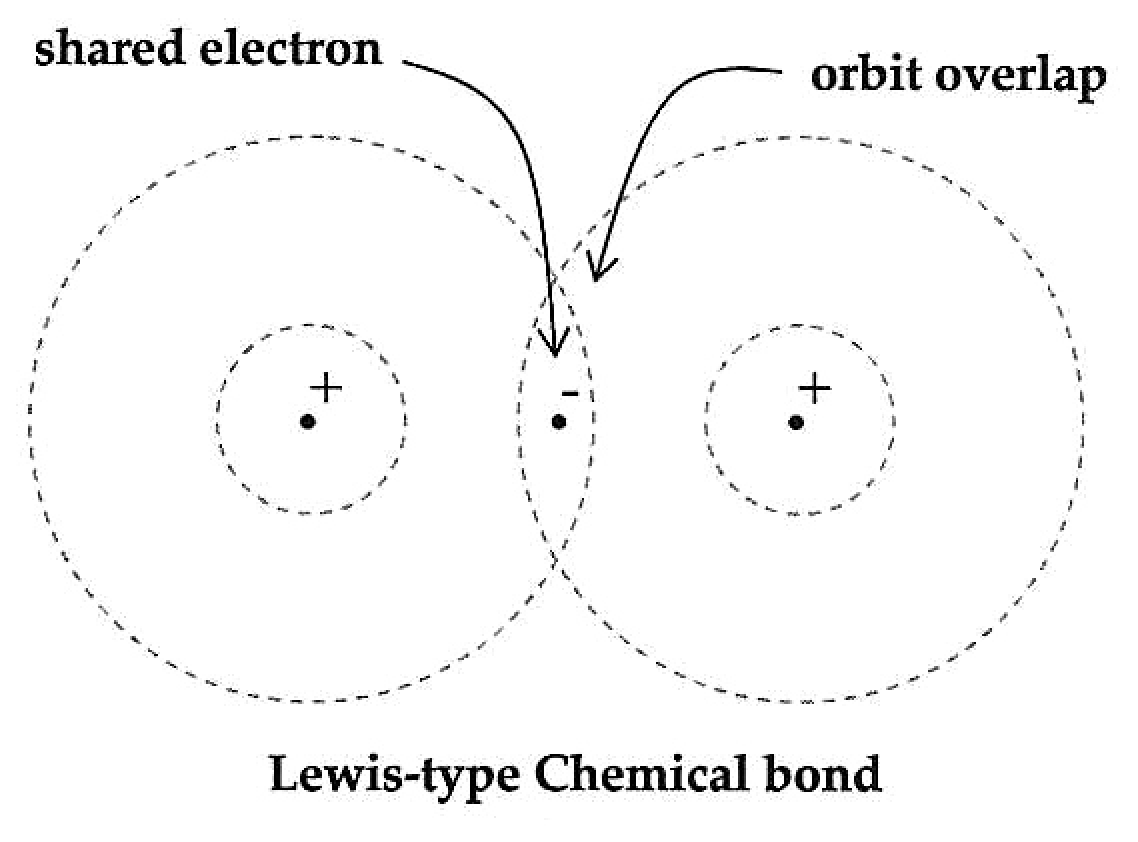
\includegraphics[scale=0.20]{figs/intro3}
\end{figure}

\begin{center}
{\footnotesize G. N. Lewis: ``An electron may form a part of the shell of two different atoms and cannot be said to belong to either one exclusively.''}
\end{center}

\end{frame}

\scriptsize

\opage{
\begin{columns}
\begin{column}{9cm}
\otitle{3.1 Molecules and the Born-Oppenheimer approximation}

\otext
Because electrons are much heavier than nuclei, the Schr\"odinger equation can be approximately separated into the nuclear and the electron parts. Thus the electronic Schr\"odinger equation for a molecule can be solved separately at each fixed nuclear configuration. This is called the Born-Oppenheimer approximation.

\otext
In the following, we will consider the simplest molecule H$_2^+$, which contains only one electron. This simple system will demonstrate the basic concepts in chemical bonding. The Schr\"odinger equation for H$_2^+$ is:

\aeqn{11.1}{H\psi(\vec{r}_1,\vec{R}_A,\vec{R}_B) = E\psi(\vec{r}_1,\vec{R}_A,\vec{R}_B)}

where $\vec{r}_1$ is the vector locating the (only) electron and $\vec{R}_A$ and $\vec{R}_B$
are the positions of the two protons. The Hamiltonian for H$_2^+$ is:

\aeqn{11.2}{\hat{H} = -\frac{\hbar^2}{2M}(\Delta_A + \Delta_B) - \frac{\hbar^2}{2m_e}\Delta_e
+ \frac{e^2}{4\pi\epsilon_0}\left(\frac{1}{R} - \frac{1}{r_{1A}} - \frac{1}{r_{1B}}\right)}

where $M$ is the proton mass, $m_e$ is the electron mass, $r_{1A}$ is the distance between the electron and nucleus A, $r_{1B}$ is the distance between the electron and nucleus B and $R$ is the A - B distance.
\end{column}
\vline\hspace*{0.1cm}
\begin{column}{3cm}
\operson{max_born}{0.20}{Max Born (1882 - 1970), German physicist and Mathematician, Nobel Prize 1954.}
\operson{robert_oppenheimer}{0.09}{Robert Oppenheimer (1904 - 1967) American theoretical physicist, ``the father of atomic bomb''}
\end{column}
\end{columns}
}

\opage{
\otext
Note that the Hamiltonian includes also the quantum mechanical kinetic energy for the protons. As such the wavefunction depends on $\vec{r}_1$, $\vec{R}_A$ and $\vec{R}_B$. Because the nuclear mass $M$ is much larger than the electron mass $m_e$, the wavefunction can be separated (Born-Oppenheimer approximation):

\aeqn{11.3}{\psi(\vec{r}_1,\vec{R}_A,\vec{R}_B) = \psi_e(\vec{r}_1, R)\psi_n(\vec{R}_A, \vec{R}_B)}

where $\psi_e$ is the electronic wavefunction that depends on the distance $R$ between the nuclei and $\psi_n$ is the nuclear wavefunction depending on $\vec{R}_A$ and $\vec{R}_B$. It can be shown that the nuclear part can be often be separated into vibrational, rotational and translational parts. The electronic Schr\"odinger equation can now be written as:

\aeqn{11.4}{\hat{H}_e\psi_e = E_e\psi_e}

Note that Eq. (\ref{eq11.4}) depends parametrically on $R$ (``one equation for each value of $R$''). The \textit{electronic Hamiltonian} is:

\aeqn{11.5}{\hat{H}_e = -\frac{\hbar^2}{2m_e}\Delta_e + \frac{e^2}{4\pi\epsilon_0}
\left(\frac{1}{R} - \frac{1}{|r_1 - R_A|} - \frac{1}{|r_1 - R_B|}\right)}

Because $R$ is a parameter, both $E_e$ and $\psi_e$ are functions of $R$.

}

\opage{
\otitle{3.2 The second law of thermodynamics}

\begin{columns}

\begin{column}{7cm}
\otext
Definition of entropy ($S$): 

\aeqn{3.8}{dS = \frac{\inex{dq}_{rev}}{T}}

\aeqn{3.9}{\Delta S = \int\frac{\inex{dq}_{rev}}{T}}

Integration of entropy over closed loops yield zero because $dS$ is an exact differential ($S$ is a state function):
\end{column}

\begin{column}{3cm}
\operson{clausius}{0.17}{Rudolph Clausius, German physicist and mathematician (1822 - 1888)}
\end{column}
\end{columns}

\aeqn{3.11}{\oint\frac{\inex{dq}_{rev}}{T} = \oint dS = 0}

In general, we have the following inequality (i.e. $\inex{dq}$ reversible or irreversible):

\aeqn{3.14}{0 = \oint dS = \oint \frac{\inex{dq}_{rev}}{T} \ge \oint\frac{\inex{dq}}{T}}

The inequality can also be written in differential form:

\aeqn{3.15}{dS \ge \frac{\inex{dq}}{T}}

For an isolated system, the inequality simplifies to:

\aeqn{3.15a}{dS \ge 0}

}

\opage{

\otext
The idea behind Clausius inequality (\ref{eq3.15a}) can be understood by considering the following example:

\ofig{entropy}{0.5}{}

\aeqn{3.25}{dS = dS_c + dS_h = \inex{dq}\times\left(\frac{1}{T_c} - \frac{1}{T_h}\right) \ge 0}

Thus we conclude that in presence of spontaneous (irreversible) processes we have $dS > 0$. At thermal equilibrium we would have $T_h = T_c$ and $dS = 0$. We will return to justification of Eq. (\ref{eq3.15}) later (non-isolated system).

}

\opage{

\otext
The second law of thermodynamics consists of two statements:

\begin{enumerate}
\item There is a state function called the entropy $S$ that can be calculated from $dS = dq_{rev} / T$.
\item The change in entropy in any process is given by $dS \ge \inex{dq} / T$, where the '$>$' sign applies to a spontaneous (irreversible; $\inex{dq}_{irrev}$) process and the equality for a reversible process ($\inex{dq}_{rev}$). In order to calculate $\Delta S$, one must use a reversible process.
\end{enumerate}

\underline{Justification for the Clausis inequality $dS \ge \frac{\inex{dq}}{T}$ (Eq. (\ref{eq3.15})):}

\begin{enumerate}

\item If the process is reversible then by definition $dS = \frac{\inex{dq}_{rev}}{T}$.

\item If the process is irreversible, we need to show that $dS > \frac{\inex{dq}_{irrev}}{T}$. Consider only $PV$-work and then the 1st law is $dU = \inex{dq} - P_{ext}dV$. For a reversible process this gives: $dU = \inex{dq}_{rev} - PdV$ and for an irreversible process: $dU = \inex{dq}_{irrev} - P_{ext}dV$. Since $dU$ is exact, the previous $dU$'s must be equal (consider integration over short paths): $\inex{dq}_{rev} - PdV = \inex{dq}_{irrev} - P_{ext}dV$. Rearranging gives: $\inex{dq}_{rev} - \inex{dq}_{irrev} = (P - P_{ext})dV$. If $P - P_{ext} > 0$ the system will expand spontaneously and $dV > 0$.  If $P - P_{ext} < 0$ the system will contract spontaneously and $dV < 0$. In both cases  $\inex{dq}_{rev} - \inex{dq}_{irrev} > 0$. Dividing boths sides by $T$ gives $\frac{\inex{dq}_{rev}}{T} - \frac{\inex{dq}_{irrev}}{T} > 0$. By using the definition of entropy (Eq. (\ref{eq3.8})) we get: $dS > \frac{\inex{dq}_{irrev}}{T}$.

\end{enumerate}

}

\opage{

\otext
Another way to state the 2nd law of thermodynamics: ``The entropy increases in a spontaneous process in an isolated system''. The entropy increases as long as spontaneous processes proceed. When the system does not change any more, the entropy will have its maximum value and we have $dS = 0$. \textit{The entropy change tells us whether a process or chemical reaction can occur spontaneously in an isolated system.} Consider an isolated system (consisting of system and surroundings):

\vspace*{-0.4cm}

\begin{columns}

\begin{column}{6cm}
\otext

System (at $T_{syst}$) and surroundings (at $T_{surr}$):

$$dS_{total} = dS_{syst} + dS_{surr}$$
$$dq_{total} = dq_{syst} + dq_{surr} = 0 \Rightarrow dq_{syst} = -dq_{surr}$$

\end{column}

\begin{column}{3cm}
\ofig{entropy2}{0.4}{}
\end{column}
\end{columns}

The total entropy cannot decrease: $dS_{total} = dS_{syst} + dS_{surr} \ge 0$ (Eq. (\ref{eq3.15a})). For the system we have: $dS_{syst} = dq / T_{syst}$ and for the surroundings: $dS_{surr} = -dq / T_{surr}$. Therefore we have:

\aeqn{3.21}{dS_{syst} \ge \frac{dq}{T_{surr}}}

\underline{Note:} The equal sign case only applies for reversible processes in Eq. (\ref{eq3.21}). The equal sign would also then apply in $dS_{total} = dS_{syst} + dS_{surr} = 0$ (reversible process).

}

\opage{

\otext
Based on changes in entropy, we can identify three different cases:

\ceqn{3.23}{(1)\textnormal{ }dS > \inex{dq} / T\textnormal{ spontaneous (irreversible) process}}
{(2)\textnormal{ }dS = \inex{dq}/T\textnormal{ reversible process (``nearly equlibrium'')}}
{(3)\textnormal{ }dS < \inex{dq} / T\textnormal{ impossible process (``forced process'')}}

For an isolated system ($dq = 0$), we have:

\ceqn{3.24}{(1)\textnormal{ }dS > 0\textnormal{ spontaneous (irreversible) process}}
{(2)\textnormal{ }dS = 0\textnormal{ reversible process (``nearly equilibrium'')}}
{(3)\textnormal{ }dS < 0\textnormal{ impossible process (``forced process'')}}

Because $S$ is a state function, it can be integrated between any two states of the system:

\aeqn{3.27}{\int\limits_{S_1}^{S_2}dS = \int\limits_{q_1}^{q_2}\frac{\inex{dq}_{rev}}{T} = S_2 - S_1 = \Delta S}

The integration path in Eq. (\ref{eq3.27}) must be reversible. This equation can be applied to irreversible processes only if a path consisting of reversible segments, can be constructed. Note that there is no entropy change for a reversible adiabatic process.

}

\opage{

\otext
\textbf{Example.} Is the expansion of a monoatomic ideal gas into a larger volume thermodynamically spontaneous? More specifically, consider reversible and isothermal expansion of an isolated ideal gas ($n = 1$ mol) initially at 298 K into a volume that is twice as large as its initial volume.

\vspace*{0.2cm}

\textbf{Solution.} Recall from Eq. (\ref{eq2.35}) that the reversible work done is ($n = 1$ mol):

$$w_{rev} = -\int\limits_{V_1}^{V_2}P_{ext}dV = -\int\limits_{V_1}^{V_2}PdV = -\int\limits_{V_1}^{V_2}\frac{nRT}{V}dV = -nRT\ln\left(\frac{V_2}{V_1}\right) = -RT\ln(2)$$

The internal energy of a monoatomic ideal gas does not depend on volume (Eq. (\ref{eq2.69})). Thus we have $\Delta U = q_{rev} + w_{rev} = 0$ and further $q_{rev} = -w_{rev} = RT\ln(2)$. Eq. (\ref{eq3.9}) with constant $T$ states that $\Delta S = \frac{q_{rev}}{T} = R\ln(2) > 0$ where we used the fact that $V_2 = 2 \times V_1$. Because the entropy change is positive, the change is spontaneous (as we already knew in practice). For the reverse process we would have $\Delta S < 0$, which means that it does not happen (unless forced).

}

\opage{

\otext

\underline{Note:} The previous problem has nothing to do with minimizing the energy, which is constant during the process. The process is purely entropy driven and is related to decrease in ``order'' at larger volume. By order we mean the arrangement of atoms or molecules. For example, $S_{gas} > S_{liquid} > S_{solid}$.

\vspace*{0.2cm}

\textbf{Example.} Calculate the entropy change when argon at 25 \degree C and 1.00 atm in a container of volume 500 cm$^3$ is allowed to expand to 1000 cm$^3$. Assume that argon behaves according to the ideal gas law.

\vspace*{0.2cm}

\textbf{Solution.} From the ideal gas law we can calculate the amount of substance:

$$n = \frac{PV}{RT} = 0.0204\textnormal{ mol}$$

In previous example we had $n = 1$. If the same calculation is carried out with $n$ in place, we have:

$$\Delta S = nR\ln\left(\frac{V_2}{V_1}\right) = nR\ln(2) = 0.118\textnormal{ J K}^{-1}$$

}

\opage{
\otitle{3.3 Energy of the hydrogen molecule ion}

\otext
Using a linear combination of atomic orbitals, it is possible to calculate the best values, in terms of energy, for the coefficients $c_1$ and $c_2$. Remember that this linear combination can only provide an approximate solution to the H$_2^+$ Schr\"odinger equation. The variational principle (see Eq. (\ref{eq10.58})) provides a systematic way to calculate the energy when $R$ (the distance between the nuclei) is fixed:

\beqn{11.14}{
E = \frac{\int\psi_g^*\hat{H}_e\psi_gd\tau}{\int\psi_g^*\psi_gd\tau} = 
\frac{\int (c_11s_A + c_21s_B)\hat{H}_e(c_11s_A + c_21s_B)d\tau}
{\int (c_11s_A + c_21s_B)^2d\tau}}
{
= \frac{c_1^2H_{AA} + 2c_1c_2H_{AB} + c_2^2H_{BB}}
{c_1^2\umark{S_{AA}}{= 1} + 2c_1c_2\umark{S_{AB}}{= S} + c_2^2\umark{S_{BB}}{= 1}}
}

where $H_{AA}$, $H_{AB}$, $H_{BB}$, $S_{AA}$, $S_{AB}$ and $S_{BB}$ have been 
used to denote the integrals occurring in Eq. (\ref{eq11.14}). The integrals $H_{AA}$
and $H_{BB}$ are called the \textit{Coulomb integrals} (sometimes generally termed as matrix elements). This interaction is attractive and therefore its numerical value must be negative. Note that by symmetry 
$H_{AA} = H_{BB}$. The integral $H_{AB}$ is called the \textit{resonance integral}
and also by symmetry $H_{AB} = H_{BA}$.

\otext
To minimize the energy expectation value in Eq. (\ref{eq11.14}) with respect to $c_1$ and $c_2$, we have to calculate the partial derivatives of energy with respect to these parameters:

}

\opage{

\aeqn{11.19}{E\times (c_1^2 + 2c_1c_2S + c_2^2) = c_1^2H_{AA} + 2c_1c_2H_{AB} + c_2^2H_{BB}}

Both sides can be differentiated with respect to $c_1$ to give:

\aeqn{11.20}{E\times (2c_1 + 2c_2S) + \frac{\partial E}{\partial c_1}\times (c_1^2 + 2c_1c_2S + c_2^2) = 2c_1H_{AA} + 2c_2H_{AB}}

In similar way, differentiation with respect to $c_2$ gives:

\aeqn{11.21}{E\times (2c_2 + 2c_1S) + \frac{\partial E}{\partial c_2}\times (c_1^2 + 2c_1c_2S + c_2^2) = 2c_2H_{BB} + 2c_1H_{AB}}

At the minimum energy (for $c_1$ and $c_2$), the partial derivatives must be zero:

\aeqn{11.22}{c_1(H_{AA} - E) + c_2(H_{AB} - SE) = 0}
\aeqn{11.23}{c_2(H_{BB} - E) + c_1(H_{AB} - SE) = 0}

In matrix notation this is (a generalized matrix eigenvalue problem):

\aeqn{11.23a}{\begin{pmatrix}H_{AA} - E & H_{AB} - SE\\
H_{AB} - SE & H_{BB} - E\\
\end{pmatrix}\begin{pmatrix} c_1\\ c_2\\\end{pmatrix} = 0}

From linear algebra, we know that a non-trivial solution exists only if:

\aeqn{11.24}{\begin{vmatrix}H_{AA} - E & H_{AB} - SE\\
H_{AB} - SE & H_{BB} - E\\
\end{vmatrix} = 0}

}

\opage{

It can be shown that $H_{AA} = H_{BB} = E_{1s} + J(R)$, where $E_{1s}$ is the energy
of a single hydrogen atom and $J(R)$ is a function of internuclear distance $R$:

\aeqn{11.25}{J(R) = e^{-2R}\left( 1 + \frac{1}{R}\right)}

Furthermore, $H_{AB} = H_{BA} = E_{1s}S(R) + K(R)$, where $K(R)$ is also a function of $R$:

\aeqn{11.26}{K(R) = \frac{S(R)}{R} - e^{-R}\left( 1 + R\right)}

If these expressions are substituted into the previous secular determinant, we get:

\aeqn{11.27}{\begin{vmatrix}E_{1s} + J - E & E_{1s}S + K - SE\\
E_{1s}S + K - SE & E_{1s} + J - E\\
\end{vmatrix} = (E_{1s} + J - E)^2 - (E_{1s}S + K - SE)^2 = 0}

This equation has two roots:

\aeqn{11.28}{E_g(R) = E_{1s} + \frac{J(R) + K(R)}{1 + S(R)}}

\aeqn{11.29}{E_u(R) = E_{1s} + \frac{J(R) - K(R)}{1 - S(R)}}

}

\opage{

\otext
Since energy is a relative quantity, it can be expressed relative to separated
nuclei:

\aeqn{11.30}{\Delta E_g(R) = E_g(R) - E_{1s} = \frac{J(R) + K(R)}{1 + S(R)}}

\aeqn{11.31}{\Delta E_u(R) = E_u(R) - E_{1s} = \frac{J(R) - K(R)}{1 - S(R)}}

The energies of these states are plotted in the figure below.\vspace{0.45cm}

\ofig{energy}{0.35}{Energies of the bonding and antibonding states in H$_2^+$.}

}

\opage{

\otext
These values can be compared with experimental results. The calculated 
ground state equilibrium bond length is 132 pm whereas the experimental value is 106 pm. The
binding energy is 170 kJ mol$^{-1}$ whereas the experimental value is 258 kJ 
mol$^{-1}$. The excited state (labeled with $u$) leads to repulsive behavior at
all bond lengths $R$ (i.e. antibonding). Because the $u$ state lies higher
in energy than the $g$ state, the $u$ state is an excited state of H$_2^+$.
This calculation can be made more accurate by adding more than two terms to
the linear combination. This procedure would also yield more excited state 
solutions. These would correspond $u$/$g$ combinations of $2s$, $2p_x$,
$2p_y$, $2p_z$ etc. orbitals.

\otext
It is a common practice to represent the molecular orbitals by molecular 
orbital (MO) diagrams:

\ofig{modiag}{0.4}{MO diagram showing the $\sigma_g$ and $\sigma_u$ molecular orbitals.}

}

\opage{

\otext
The formation of bonding and antibonding orbitals can be visualized as follows:

\ofig{moformation}{0.33}{}
}

\opage{

\otext
\underline{1. $\sigma$ orbitals.} When two $s$ or $p_z$ orbitals interact,
a $\sigma$ molecular orbital is formed. The notation $\sigma$ specifies
the amount of angular momentum about the molecular axis (for $\sigma$, $\lambda = 0$ with $L_z = 
\pm\lambda\hbar$). In many-electron systems, both bonding and antibonding $\sigma$ 
orbitals can each hold a maximum of two electrons. Antibonding orbitals are often 
denoted by *.

\otext
\underline{2. $\pi$ orbitals.} When two $p_{x,y}$ orbitals interact, a $\pi$ molecular orbital forms. $\pi$-orbitals are doubly degenerate: $\pi_{+1}$ and $\pi_{-1}$ (or alternatively $\pi_x$ and $\pi_y$), where the $+1/-1$ refer to the eigenvalue of the $L_z$ operator ($\lambda = \pm1$). In many-electron systems a bonding $\pi$-orbital can therefore hold a maximum of 4 electrons (i.e. both $\pi_{+1}$ and $\pi_{-1}$ each can hold two electrons). The same holds for the antibonding $\pi$ orbitals. Note that only the atomic orbitals of the same symmetry mix to form molecular orbitals (for example, $p_z - p_z$, $p_x -  p_x$ and $p_y - p_y$). When atomic $d$ orbitals mix to form molecular orbitals, $\sigma (\lambda = 0)$, $\pi (\lambda = \pm 1)$ and $\delta (\lambda = \pm 2)$ MOs form. 

\otext
Excited state energies of H$_2^+$ resulting from a calculation employing an extended basis set (e.g. more terms in the LCAO) are shown on the left below. The MO energy diagram, which includes the higher energy molecular orbitals, is shown on the right hand side. Note that the energy order of the MOs depends on the molecule.

}

\opage{
\begin{columns}
\begin{column}{6cm}
\ofig{energy2}{0.4}{The lowest excited states of H$_2^+$.}
\end{column}
\begin{column}{6cm}
\ofig{modiag2}{0.4}{\hspace{-0.5cm}MO diagram for homonuclear diatomic molecules.}
\end{column}
\end{columns}
}

\opage{
\otitle{3.4 Molecular orbital description of hydrogen molecule}

\otext
Using the Born-Oppenheimer approximation, the electronic Hamiltonian for H$_2$ molecule can be written as:

\aeqn{11.37}{H = -\frac{\hbar^2}{2m_e}\left( \Delta_1 + \Delta_2\right)
+ \frac{e^2}{4\pi\epsilon_0}\left(\frac{1}{R} + \frac{1}{r_{12}} - \frac{1}{r_{A1}} 
- \frac{1}{r_{A2}} - \frac{1}{r_{B1}} - \frac{1}{r_{B2}}\right)}

The distances between the electrons and the nuclei are indicated below.

\vspace{-0.6cm}
\ofig{distances}{0.5}{}

\vspace{-0.4cm}
The main difficulty in the Hamiltonian of Eq. (\ref{eq11.37}) is the $1/r_{12}$
term, which connects the two electrons to each other. This means that a simple 
product wavefunction is not sufficient. No known analytic solutions have been 
found to the electronic Schr\"odinger equation of H$_2$. For this reason, we will
attempt to solve the problem approximately by using the LCAO-MO approach that we 
used previously. For example, the ground state for H$_2$ is obtained by placing 
two electrons with opposite spins on the 1$\sigma_g$ orbital. This assumes that
the wavefunction is expressed as antisymmetrized product (e.g. a Slater determinant).

}

\opage{
\otext
According to the Pauli principle, two electrons with opposite spins can be assigned
to a given spatial orbital. As a first approximation, we assume that the molecular
orbitals in H$_2$ remain the same as in H$_2^+$. Hence we can say that both
electrons occupy the 1$\sigma_g$ orbital (the ground state) and the electronic
configuration is denoted by (1$\sigma_g$)$^2$. This is a similar notation 
that we used previously for atoms (for example, He atom is ($1s$)$^2$).

\otext
The molecular orbital for electron 1 in 1$\sigma_g$ molecular orbital is (see Eq. (\ref{eq11.11})):

\aeqn{11.39}{1\sigma_g(1) = \frac{1}{\sqrt{2(1 + S)}}(1s_A(1) + 1s_B(1))}

\otext
In Eq. (\ref{eq10.78}) we found that the total wavefunction must be antisymmetric
with respect to change in electron indices. This can be achieved by using the 
Slater determinant:

\aeqn{11.40}{\psi_{MO}^{(1\sigma_g)^2} = \frac{1}{\sqrt{2}}\begin{vmatrix}
1\sigma_g(1)\alpha (1) & 1\sigma_g(1)\beta (1)\\
1\sigma_g(2)\alpha (2) & 1\sigma_g(2)\beta (2)\\
\end{vmatrix}
}

where $\alpha$ and $\beta$ denote the electron spin. The Slater determinant can be
expanded as follows:

}

\opage{

\beqn{11.41}
{\psi_{MO}^{(1\sigma_g)^2} = \frac{1}{\sqrt{2}} 
 (1\sigma_g(1)1\sigma_g(2)\alpha (1)\beta (2) 
- 1\sigma_g(1)1\sigma_g(2)\beta (1)\alpha (2))}
{= \frac{1}{2\sqrt{2}(1 + S_{AB})}(1s_A(1) + 1s_B(1))(1s_A(2) + 1s_B(2))
(\alpha (1)\beta (2) - \alpha (2)\beta (1))}

\otext
Note that this wavefunction is only approximate and is definitely not an 
eigenfunction of the H$_2$ electronic Hamiltonian. Thus we must calculate the 
electronic energy by taking an expectation value of this wavefunction with the
Hamiltonian given in Eq. (\ref{eq11.37}) (the actual calculation not shown):

\aeqn{11.42}{E(R) = 2E_{1s} + \frac{e^2}{4\pi\epsilon_0 R} 
- \textnormal{``integrals''}}

\otext
where $E_{1s}$ is the electronic energy of one hydrogen atom. The second term 
represents the Coulomb repulsion between the two positively charged nuclei and
the last term (``integrals'') contains a series of integrals describing the 
interactions of various charge distributions with one another (see P. W. 
Atkins, Molecular Quantum Mechanics, Oxford University Press). With this 
approach, the minimum energy is reached at $R$ = 84 pm (experimental 74.1 pm)
and dissociation energy $D_e$ = 255 kJ mol$^{-1}$ (experimental 458 kJ 
mol$^{-1}$).

}

\opage{

\otext
This simple approach is not very accurate but it demonstrates that the method 
works. To improve the accuracy, ionic and covalent terms should be considered
separately:

\aeqn{11.34}{\umark{1s_A(1)1s_A(2)}{\textnormal{Ionic (H$^-$ + H$^+$)}}
+ \umark{1s_A(1)1s_B(2) + 1s_A(2)1s_B(1)}{\textnormal{Covalent (H + H)}}
+ \umark{1s_B(1)1s_B(2)}{\textnormal{Ionic (H$^+$ + H$^-$)}}}

Both covalent and ionic terms can be introduced into the wavefunction with their 
own variational parameters $c_1$ and $c_2$:

\aeqn{11.44}{\psi = c_1\psi_\textnormal{covalent} + c_2\psi_\textnormal{ionic}}

\aeqn{11.45}{\psi_\textnormal{covalent} = 1s_A(1)1s_B(2) + 1s_A(2)1s_B(1)}

\aeqn{11.46}{\psi_\textnormal{ionic} = 1s_A(1)1s_A(2) + 1s_B(1)1s_B(2)}

\otext
\vspace{-0.3cm}
Note that the variational constants $c_1$ and $c_2$ depend on the 
internuclear distance $R$. Minimization of the energy expectation value with 
respect to these constants gives $R_e$ = 74.9 pm (experiment 74.1 pm) and $D_e$
= 386 kJ mol$^{-1}$ (experiment 458 kJ mol$^{-1}$). Further improvement could 
be achieved by adding higher atomic orbitals into the wavefunction. The 
previously discussed Hartree-Fock method provides an efficient way for
solving the problem. Recall that this method is only approximate as it ignores 
the electron-electron correlation effects completely. The full treatment 
requires use of configuration interaction methods, which can yield essentially 
exact results: $D_e$ = 36117.8 cm$^{-1}$ (CI) vs. 36117.3$\pm$1.0 cm$^{-1}$ 
(exp) and $R_e$ = 74.140 pm vs. 74.139 pm (exp).

}

\opage{

\ofig{h2}{0.6}{Some of the lowest lying excited states of H$_2$.}

}

\opage{

\otext
In diatomic (and linear) molecules, the quantization axis is chosen along the 
molecule. When spin-orbit interaction is negligible, this allows us to define 
the total orbital and spin angular momenta about the molecular axis:

\aeqn{11.48}{\Lambda = \left|m_1 + m_2 + ...\right|}

where $m_i = 0$ for a $\sigma$ orbital, $m_i = \pm 1$ for a $\pi$ orbital, 
$m_i = \pm 2$ for a $\delta$ orbital, etc. The value of $\Lambda$ is
expressed using the following capital Greek letters (just like we had $s$, $p$, $d$ for 
atoms):

\begin{center}
\begin{tabular}{lllllll}
$\Lambda$ & = & 0 & 1 & 2 & 3 & ...\\
Symbol & = & $\Sigma$ & $\Pi$ & $\Delta$ & $\Phi$ & ...\\
\end{tabular}
\end{center}

The state multiplicity is given by $2S + 1$ where $S$ is the sum of the electron spins in the molecule. The term symbol for a diatomic molecule is represented by:

\aeqn{11.49}{^{2S+1}\Lambda}

\otext
\vspace{-0.4cm}
\textbf{Example.} What is the term symbol for ground state H$_2$?

\otext
\textbf{Solution.} Both electrons are on a $\sigma$ orbital and hence $m_1 = m_2
= 0$. This gives $\Lambda = 0$, which corresponds to $\Sigma$. The electrons 
occupy the same molecular orbital with opposite spins and hence $2S + 1 = 1$.
This gives the term symbol as $^1\Sigma$.

}

\opage{

\otext
For $\Sigma$ terms superscripts ``$+$'' and ``$-$'' are used to express the
parity of the wavefunction with respect to reflection in the plane 
containing the internuclear axis. For example, for ground state H$_2$, we would
have a ``$+$'' symbol. As we have seen before, orbitals in diatomic molecules may be 
characterized by the $g$/$u$ labels. These labels are often added to term
symbols as subscripts. If only one unpaired electron is present, the $u$/$g$
label reflects the symmetry of the unpaired electron orbital. Closed shell 
molecules have always $g$. With more than one unpaired electron, the overall
parity should be calculated using the following rules: $g \times g = g$, $g \times 
u = u$, $u \times g = u$ and $u \times u = g$.

\otext
\textbf{Example.} What is the term symbol for ground state O$_2$?

\otext
\textbf{Solution.} Ground state $O_2$ has two electrons with parallel spins on the $\pi_{+1}$ and $\pi_{-1}$ orbitals. Thus this is a triplet state molecule with the orbital angular momentum from the two $\pi$-electrons being cancelled. This gives a $^3\Sigma$ term.  The two $\pi$'s are anti-bonding and as such they are desginated as $g$ and further $g\times g = g$ (remember that for $\pi$ orbigals the $g/u$ vs. bonding/anti-bonding is reversed from that of $\sigma$ orbitals). To see the $+/-$ symmetry, it is convenient to think about $\pi_x$ and $\pi_y$ Cartesian orbitals (draw a picture!) and see that one of them is $+$ and the other is $-$ (they are perpendicular to each other). Again $+ \times - = -$ and we have the complete term symbol as $^3\Sigma_g^-$.

}

\opage{

\otext
\underline{Notes:}\\
\vspace{0.4cm}
\begin{itemize}
\item When spin-orbit interaction is small, the above term symbols are 
adequate (``Hund's case (a)'').\\
\item When spin-orbit interaction is large, $S$ and $\Lambda$ can no longer be 
specified but their sum $J = |S + \Lambda|$ is a good quantum number.\\
\end{itemize}

}

\opage{
\otitle{3.5 Electron configurations of homonuclear diatomic molecules}

\begin{columns}
\begin{column}{5.5cm}

\vspace{-1.0cm}

\otext
Which atomic orbitals mix to form molecular orbitals and what are their
relative energies? The graph on the left can be used to obtain the energy order
of molecular orbitals and indicates the atomic orbital limits.\\

\vspace{0.5cm}
\otext
\underline{The non-crossing rule:} States with the same symmetry never cross.\\

\vspace{0.5cm}
\otext
\begin{tabular}{ll}
Bonding orbitals: & $1\sigma_g$, $2\sigma_g$, 1$\pi_u$, etc.\\
Antibonding orbitals: & $1\sigma_u^*$, $2\sigma_u^*$, $1\pi_g^*$, etc.\\
\end{tabular}

\vspace{0.5cm}
\textbf{Note that the $u$/$g$ labels are reversed for bonding/antibonding $\pi$ orbitals!}
\end{column}
\begin{column}{6.5cm}
\vspace{-0.8cm}
\ofig{correlation}{0.27}{}
\end{column}
\end{columns}
}

\opage{

\otext
The orbitals should be filled with electrons in the order of increasing energy. 
Note that $\pi$, $\delta$, etc. orbitals can hold a total of 4 electrons. If only 
one bond is formed, we say that the bond order (BO) is 1. If two bonds form (for 
example, one $\sigma$ and one $\pi$), we say that the bond order is 2 (double bond). 
Molecular orbitals always come in pairs: bonding and antibonding.

\begin{table}
\label{table1}
\begin{tabular}{lllllll}
Molecule & \# of els. & El. Conf. & Term sym. & BO & $R_e$ (\AA) & $D_e$ (eV) \\
H$_2^+$ & 1 & $(1\sigma_g)$ & $^2\Sigma_g$ & 0.5 & 1.060 & 2.793\\
H$_2$   & 2 & $(1\sigma_g)^2$ & $^1\Sigma_g$ & 1.0 & 0.741 & 4.783\\
He$_2^+$& 3 & $(1\sigma_g)^2(1\sigma_u)$ & $^2\Sigma_u$ & 0.5 & 1.080 & 2.5\\
He$_2$  & 4 & $(1\sigma_g)^2(1\sigma_u)^2$ & $^1\Sigma_g$ & 0.0 & 
\multicolumn{2}{c}{Not bound}\\
Li$_2$  & 6 & He$_2(2\sigma_g)^2$ & $^1\Sigma_g$ & 1.0 & 2.673 & 1.14\\
Be$_2$  & 8 & He$_2(2\sigma_g)^2(2\sigma_u)^2$ & $^1\Sigma_g$ & 0.0 & 
\multicolumn{2}{c}{Not bound}\\
B$_2$   & 10 & Be$_2(1\pi_u)^2$ & $^3\Sigma_g$ & 1.0 & 1.589 & $\approx$3.0\\
C$_2$   & 12 & Be$_2(1\pi_u)^4$ & $^1\Sigma_g$ & 2.0 & 1.242 & 6.36\\
N$_2^+$ & 13 & Be$_2(1\pi_u)^4(3\sigma_g)$ & $^2\Sigma_g$ & 2.5 & 1.116 & 8.86\\
N$_2$ & 14 & Be$_2(1\pi_u)^4(3\sigma_g)^2$ & $^1\Sigma_g$ & 3.0 & 1.094 & 9.902\\
O$_2^+$ & 15 & N$_2(1\pi_g)$ & $^2\Pi_g$ & 2.5 & 1.123 & 6.77\\
O$_2$ & 16 & N$_2(1\pi_g)^2$ & $^3\Sigma_g$ & 2.0 & 1.207 & 5.213\\
F$_2$ & 18 & N$_2(1\pi_g)^4$ & $^1\Sigma_g$ & 1.0 & 1.435 & 1.34\\
Ne$_2$ & 20 & N$_2(1\pi_g)^4(3\sigma_u)^2$ & $^1\Sigma_g$ & 0.0 &
\multicolumn{2}{c}{Not bound}\\
\end{tabular}
\end{table}

Note that the Hund's rules predict that the electron configuration with the
largest multiplicity lies the lowest in energy when the highest occupied
MOs are degenerate.

}

\opage{
\otitle{3.6 The angular momentum of the particle}

\otext
The quantum numbers $l$ and $m_l$ are directly related to the magnitude and projected value of angular momentum. To see this, we first use expressions from classical physics. The rotational energy is given by $E = \frac{1}{2}I\omega^2 = \frac{l^2}{2m}$ where $I$ is the moment of inertia, $\omega$ is the angular momentum and $l$ is the magnitude of the angular momentum. If one compares this expression with Eq. (\ref{eq3.24}) we get:

\aeqn{3.25}{\left|l\right| = \sqrt{l(l+1)}\hbar\textnormal{ or }l^2 = l(l+1)\hbar^2}

where $\left|l\right|$ denotes the magintude of angular momentum. This is why $l$ is called the \textit{angular momentum quantum number} as it is directly related to the magnitude of angular momentum. The spherical harmonics are also eigenfunctions of $l_z$:

\aeqn{3.26}{l_zY_{l,m_l} = \frac{\hbar}{i}\left(\Theta_{l,m_l}\frac{e^{im_l\phi}}{\sqrt{2\pi}}\right) = m_l\hbar Y_{l,_l}}

which shows that $m_l$ specifies the projection of angular momentum on the $z$-axis. Because $m_l$ is restricted to only certain values, $l_z$ must also obey this restriction (\textit{space quantitization}). The term space quantitization follows from the vector model of angular momentum:

}

\opage{

\otext

\begin{columns}

\begin{column}{4cm}
\ofig{angvec}{0.2}{}
\end{column}

\begin{column}{4cm}

\otext
The angle between the $z$-axis and the $\vec{l}$ is given by:

\aeqn{3.27}{\cos(\theta) = \frac{m_l}{\sqrt{l(l+1)}}}

Since $l_x$, $l_y$ and $l_z$ do not commute, we cannot specify $l_x$ and $l_y$ exactly. This uncertainty is drawn on the left with a circle extending around the $z$-axis.
\end{column}

\end{columns}


}

\opage{
\otitle{3.7 H\"uckel molecular orbital theory}

\begin{columns}
\begin{column}{7cm}

\otext
Molecules with extensive $\pi$ bonding systems, such as benzene,
are not described very well by the valence bond theory because the
$\pi$ electrons are delocalized over the whole molecule. $\sigma$ and $\pi$ 
bonds are demonstrated below for ehylene (C$_2$H$_4$ with $sp^2$ carbons):
\end{column}
\begin{column}{3cm}
\vspace{-0.8cm}
\operson{erich_huckel}{0.2}{Erich H\"uckel (1896 - 1980), German physical chemist.}
\end{column}
\end{columns}

\begin{columns}
\begin{column}{5.5cm}
\ofig{sigma-bond}{0.4}{Formation of $\sigma$ bonds from hybrid orbials.}
\end{column}
\begin{column}{6cm}
\vspace{-0.5cm}
\ofig{pi-bond}{0.4}{Formation of $\pi$ bond from the non-hybrid $p$-orbials.}
\end{column}
\end{columns}

\otext
Note that we have chosen $z$-axis along the internuclear axis. Because both $\sigma$ and $\pi$ bonding occurs between the two carbon atoms, we say that this is a \underline{double bond}. Note that the hybrid orbitals here also explain the geometry. For \underline{triple bonds}, one $\sigma$ and two $\pi$ bonds are formed.

}

\opage{
\otext
\textit{H\"uckel molecular orbital theory} assumes that the $\pi$ electrons, which are 
responsible for the special properties of conjugated and aromatic 
hydrocarbons, do not interact with one another and the total wavefunction is 
just a product of the one-electron molecular orbitals. The $\pi$ molecular 
orbital of the two carbons in C$_2$H$_4$ can be written approximately as:

\aeqn{11.64}{\psi = c_1\phi_1 + c_2\phi_2}

where $\phi_1$ and $\phi_2$ are the $2p_y$ atomic orbitals for carbon 1 and 2, 
respectively. By using the variational principle (see Eq. (\ref{eq11.24})) gives 
the following secular determinant:

\aeqn{11.65}{\begin{vmatrix} H_{11} - ES_{11} & H_{12} - ES_{12}\\
H_{21} - ES_{21} & H_{22} - ES_{22}\\ \end{vmatrix} = 0 \textnormal{ with }
H_{ij} = \int\phi_i^*H\phi_jd\tau \textnormal{ and } S_{ij} = \int\phi_i^*\phi_jd\tau}

In H\"uckel theory, the secular equation is simplified by assuming:

1. All the overlap integrals $S_{ij}$ are set to zero unless $i = j$, when 
$S_{ii} = 1$.\\
2. All diagonal matrix elements $H_{ii}$ are set to a constant denoted by
$\alpha$.\\
3. The resonance integrals $H_{ij}$ ($i \ne j$) are set to zero except for 
those on the neighboring atoms, which are set equal to a constant ($\beta$). Note that 
the indices here also identify atoms because the atomic orbitals are centered on atoms.\\

\otext
Now Eq. (\ref{eq11.65}) becomes:

\aeqn{11.66}{\begin{vmatrix}\alpha - E & \beta\\
\beta & \alpha - E\\ \end{vmatrix} = 0}

}

\opage{
\otext
In H\"uckel theory, the Coulomb integral $\alpha$ and the resonance integral 
$\beta$ are regarded as empirical parameters. They can be obtained, for 
example, from experimental data. Thus, in the H\"uckel theory it is not 
necessary to specify the Hamiltonian operator!
Expansion of the determinant in Eq. (\ref{eq11.66}) leads to a quadratic 
equation for $E$. The solutions are found to be $E = \alpha \pm \beta$.
In general, it can be shown that $\beta < 0$, which implies that the lowest orbital energy
is $E_1 = \alpha + \beta$. There are two $\pi$ electrons and therefore the
total energy is $E_{tot} = 2E_1 = 2\alpha + 2\beta$. Do not confuse $\alpha$ and $\beta$ here with electron spin.

\otext
The wavefunctions (i.e. the coefficients $c_1$ and $c_2$ in Eq. (\ref{eq11.64})) 
can be obtained by substituting the two values of $E$ into the original linear 
equations (cf. Eqs. (\ref{eq11.22}) and (\ref{eq11.23})):

\aeqn{11.67}{c_1(\alpha - E) + c_2\beta = 0}
\aeqn{11.68}{c_1\beta + c_2(\alpha - E) = 0}

For the lowest energy orbital ($E_1 = \alpha + \beta$), we get (including normalization):

\aeqn{11.69}{\psi_1 = \frac{1}{\sqrt{2}}(\phi_1 + \phi_2) \hspace{0.5cm}(\textnormal{i.e.}~c_1 = c_2 = \frac{1}{\sqrt{2}})}

and for the highest energy orbital ($E_2 = \alpha - \beta$) (including normalization):

\aeqn{11.70}{\psi_2 = \frac{1}{\sqrt{2}}(\phi_1 - \phi_2) \hspace{0.5cm}(\textnormal{i.e.}~c_1 = \frac{1}{\sqrt{2}}, c_2 = -\frac{1}{\sqrt{2}})}

}

\opage{
\ofig{huckel-orbitals}{0.25}{Energy level diagram showing the low energy (bonding)
and high energy (antibonding) orbitals.}

\otext
These orbitals resemble the H$_2^+$ LCAO MOs discussed previously.
This also gives us an estimate for one of the excited states where one electron
is promoted from the bonding to the antibonding orbital. The excitation energy
is found to be $2|\beta|$, which allows for, for example, estimation of $\beta$
from UV/VIS absorption spectroscopy.

\otext
\begin{tabular}{ll}
HOMO orbital & = The highest occupied molecular orbital.\\
LUMO orbital & = The lowest unoccupied molcular orbital.\\
\end{tabular}

}

\opage{
\otext
\textbf{Example.} Calculate the $\pi$ electronic energy for 1,3-butadiene 
(CH$_2$=CHCH=CH$_2$) by using the H\"uckel theory.

\otext
\textbf{Solution.} First we have to write the secular determinant using the 
rules given earlier. In order to do this, it is convenient to number the 
carbon atoms in the molecule:

\vspace{-0.5cm}
\begin{center}
$\overset{1}{\textnormal{CH}_2} = \overset{2}{\textnormal{CH}} 
- \overset{3}{\textnormal{CH}} = \overset{4}{\textnormal{CH}_2}$
\end{center}

\vspace{-0.6cm}
\otext
In this case there are two scenarios that should be considered:\\

\begin{itemize}
\item[1.] A localized solution where the $\pi$ electrons are shared either with atoms 1 and 2 or 3 and 4. This would imply that the $\beta$ parameter should not be written between nuclei 2 and 3.\\
\item[2.] A delocalized solution where the $\pi$ electrons are delocalized over all four carbons. This would imply that the $\beta$ parameters should be written between nuclei 2 and 3.\\
\end{itemize}

\vspace{-0.25cm}
\otext
Here it turns out that scenario 2) gives a lower energy solution and we will 
study that in more detail. In general, however, both cases should be considered. The 
energy difference between 1) and 2) is called the \textit{resonance stabilization 
energy}. The secular determinant is:

\begin{columns}
\begin{column}{6.5cm}
\aeqn{11.71}{
\begin{matrix}\\1\vspace{0.07cm}\\2\\3\\4\\\end{matrix}
\begin{vmatrix}
1 & 2 & 3 & 4\\
\alpha - E & \beta & 0 & 0\\
\beta & \alpha - E & \beta & 0\\
0 & \beta & \alpha - E & \beta\\
0 & 0 & \beta & \alpha - E\\
\end{vmatrix}
= 0
}
\end{column}
\begin{column}{3.5cm}
The numbers outside the determinant are just guides to see which atoms each
row/column correspond to.
\end{column}
\end{columns}

}

\opage{
\otext
To simplify notation, we divide each row by $\beta$ and denote $x = (\alpha - E) / \beta$:

\aeqn{11.72}{\begin{vmatrix}
x & 1 & 0 & 0\\
1 & x & 1 & 0\\
0 & 1 & x & 1\\
0 & 0 & 1 & x\\
\end{vmatrix} = 0}

\otext
Expansion of this determinant gives $x^4 - 3x^2 + 1 = 0$. There are four solutions $x = \pm 0.618$ and $x = \pm 1.618$. Thus there are four possible orbital energy levels:

\deqn{11.73}
{E_1 = \alpha + 1.618\beta \hspace{0.5cm}\textnormal{(lowest energy)}}
{E_2 = \alpha + 0.618\beta}
{E_3 = \alpha - 0.618\beta}
{E_4 = \alpha - 1.618\beta \hspace{0.5cm}\textnormal{(highest energy)}}

There are four $\pi$ electrons, which occupy the two lowest energy 
orbitals. This gives the total $\pi$ electronic energy for the molecule:

\aeqn{11.74}{E_\pi = 2(\alpha + 1.618\beta) + 2(\alpha + 0.618\beta)
= 4\alpha + 4.472\beta}

\otext
and the lowest excitation energy is 1.236$|\beta|$.

}

\opage{

\ofig{huckel-orbitals2}{0.3}{Note especially the delocalization of the orbitals
over the whole molecule.}

}

\opage{
\otext
The four H\"uckel MO wavefunctions are (calculations not shown):

\deqn{11.75}
{\psi_1 = 0.372\phi_1 + 0.602\phi_2 + 0.602\phi_3 + 0.372\phi_4}
{\psi_2 = 0.602\phi_1 + 0.372\phi_2 - 0.372\phi_3 - 0.602\phi_4}
{\psi_3 = 0.602\phi_1 - 0.372\phi_2 - 0.372\phi_3 + 0.602\phi_4}
{\psi_4 = 0.372\phi_1 - 0.602\phi_2 + 0.602\phi_3 - 0.372\phi_4}

\vspace*{-0.4cm}

\otext
\textbf{Example.} Apply the H\"uckel method for benzene molecule.\\

\otext
\textbf{Solution.} The secular determinant for benzene is (electrons delocalized):\\

\aeqn{11.76}{
\begin{vmatrix}
\alpha - E & \beta      &     0      & 0          & 0          & \beta\\
\beta      & \alpha - E & \beta      & 0          & 0          & 0\\
0          & \beta      & \alpha - E & \beta      & 0          & 0\\
0          & 0          & \beta      & \alpha - E & \beta      & 0\\
0          & 0          & 0          & \beta      & \alpha - E & \beta\\
\beta      & 0          & 0          & 0          & \beta      & \alpha - E\\
\end{vmatrix}
= 0
}

The solutions are (where the six $\pi$ electrons should be placed):

\vspace{-0.5cm}
\deqn{11.77}
{E_1 = \alpha + 2\beta~~\textnormal{(lowest energy)}}
{E_2 = E_3 = \alpha + \beta}
{E_4 = E_5 = \alpha - \beta}
{E_6 = \alpha - 2\beta~~\textnormal{(highest energy)}}

}

\opage{
\otitle{3.8 The rigid rotor}

\otext
Now we will apply the previous theory to describe rotation of diatomic molecule where we assume that the bond length is fixed (``rigid rotor''). The masses of the nuclei are represented by $m_1$ and $m_2$ and their separation is fixed at distance $R$. The total Hamiltonian for this probelm is:

\aeqn{3.28}{H = -\frac{\hbar^2}{2m_1}\nabla^2_1 - \frac{\hbar^2}{2m_2}\nabla_2^2}

where $\nabla_i^2$ differentiates with respect to the coordinates of particle $i$. This can be transformed as (see Atkins \& Friedman, Molecular Quantum Mechanics, Further information 4):

$$\frac{1}{m_1}\nabla_1^2 + \frac{1}{m_2}\nabla_2^2 = \frac{1}{m}\nabla_{\textnormal{cm}}^2 + \frac{1}{\mu}\nabla^2$$

The subscript cm refers to the variables describing the center of mass translational movement of the molecule, the Laplacian without subscript refers to the internal coordinates of the molecule (vibration and rotation), $m = m_1 + m_2$ and:

\aeqn{3.29}{\frac{1}{\mu} = \frac{1}{m_1} + \frac{1}{m_2}\textnormal{ or } \mu = \frac{m_1m_2}{m_1 + m_2}}

where $\mu$ is called the \textit{reduced mass}.

}

\opage{

\otext
Now we can rewrite the Schr\"odinger equation as:

\aeqn{3.30}{-\frac{\hbar^2}{2m}\nabla_{\textnormal{cm}}^2\Psi - \frac{\hbar^2}{2\mu}\nabla^2\Psi = E_{\textnormal{total}}\Psi}

Since the Hamiltonia is a sum of two terms depending on different variables, it is possible to separate this equation as:

\beqn{3.31}{-\frac{\hbar^2}{2m}\nabla^2_{\textnormal{cm}}\psi_{\textnormal{cm}} = E_{\textnormal{cm}}\psi_{\textnormal{cm}}}
{-\frac{\hbar^2}{2\mu}\nabla^2\psi = E\psi}

with $E_{\textnormal{total}} = E_{\textnormal{cm}} + E$. The first equation is related to free translation of the molecule where as the second equation describes both rotation and vibration of the (diatomic) molecule. The 2nd equation can be solved in spherical coordinates and simplified with the rigid rotor assumption ($R$ is constant). Thus the radial derivatives in the Laplacian are zero and only the angular part is retained:

\aeqn{3.32}{-\frac{\hbar^2}{2\mu R^2}\Lambda^2\psi = E\psi}

To simplify notation we write $I = \mu R^2$. This is identical to Eq. (\ref{eq3.21}). The solutions can be labelled by two quantum numbers $l$ and $m_l$, which in the context of molecular rotation, are usually written as $J$ and $M_J$. 

}

\opage{

\otext
The eigenfunctions for the rotating diatomic molecule are hence spherical harmonics $Y_{J,M_J}$ and the rotational energy levels are given by:

\aeqn{3.34}{E_{J,M_J} = J(J+1)\frac{\hbar^2}{2I}}

where $J = 0, 1, 2, ...$ and $M_J = 0, \pm 1, \pm 2, ..., \pm J$. Because the energy is independent of $M_J$, each rotational level is $2J + $ times degenerate. 

\vspace*{0.2cm}

\textbf{Example.} What are the reduced mass and moment of inertia of H$^{35}$Cl? The equilibrium internuclear distance $R_e$ is 127.5 pm (1.275 \AA). What are the values of $L, L_z$ and $E$ for the state with $J = 1$? The atomic masses are: $m_\textnormal{H} = 1.673470 \times 10^{-27}$ kg and $m_\textnormal{Cl} = 5.806496 \times 10^{-26}$ kg.\\

\vspace*{0.2cm}
\textbf{Solution.} First we calculate the reduced mass (Eq. (\ref{eq3.29})):

$$\mu = \frac{m_\textnormal{H}m_{^{35}\textnormal{Cl}}}{m_\textnormal{H} + m_{^{35}\textnormal{Cl}}} = \frac{(1.673470\times 10^{-27}\textnormal{ kg})(5.806496\times 10^{-26}\textnormal{ kg})}{(1.673470\times 10^{-27}\textnormal{ kg}) + (5.806496\times 10^{-26}\textnormal{ kg})}$$
$$= 1.62665\times 10^{-27}\textnormal{ kg}$$

}

\opage{

\otext
Next, $I = mr^2$ gives the moment of inertia:

$$I = \mu R_e^2 = (1.626\times 10^{-27}\textnormal{ kg})(127.5\times 10^{-12}\textnormal{ m})^2 = 2.644\times 10^{-47}\textnormal{ kg m}^2$$

$L$ is given by Eq. (\ref{eq3.25}):

$$L = \sqrt{J(J+1)}\hbar = \sqrt{2}\left(1.054\times 10^{-34}\textnormal{ Js}\right) = 1.491\times 10^{-34}\textnormal{ Js}$$

$L_z$ is given by Eq. (\ref{eq3.26}):

$$L_z = -\hbar,0,\hbar\textnormal{ (three possible values)}$$

Energy of the $J = 1$ level is given by Eq. (\ref{eq3.34}) (or Eq. (\ref{eq3.24})):

$$E = \frac{\hbar^2}{2I}J(J+1) = \frac{\hbar^2}{I} = 4.206\times 10^{-22}\textnormal{ J} = 21\textnormal{ cm}^{-1}$$

This rotational spacing can be, for example, observed in gas phase infrared spectrum of HCl.

}

\opage{
\otitle{3.9 Intermolecular forces}

\otext
Consider two atoms or molecules that do not form chemical bonds. When they approach
each other, a small binding (van der Waals; vdW) occurs first and after that strong 
repulsion (Pauli repulsion). The repulsion follows from the overlap of the doubly 
occupied orbitals as discussed earlier. The small vdW binding contributes to physical 
processes like freezing and boiling. At large distances, the interaction energy 
approaches zero. For example, a ``pair potential'' might look like:

\ofig{hehe}{0.25}{Pair potential between two helium atoms.}

\otext
Note that the energy unit above is K (Kelvin; i.e. multiplication by the Boltzmann constant gives energy). Very often \AA ngstr\"oms (\AA) or Bohr (atomic units; a.u.) are used for units of distance.

}

\opage{
\otext
\underline{1. Dipole - dipole interaction.} The dipole -- dipole interaction between two
freely rotating dipoles (i.e., molecules with dipole moments) is zero. However, because their mutual potential energy depends on their relative orientation, the molecules do not in fact rotate completely freely, even in gas phase. The lower energy orientations are marginally favored, so there is a nonzero average interaction between the dipoles. It can be shown that this interaction has the form (\textit{the Keesom interaction}):

\aeqn{11.83}{\left< V(R) \right>_{dd} = -\frac{2}{3kT}\left( \frac{\mu_A\mu_B}{4\pi\epsilon_0} 
\right)^2 \times \frac{1}{R^6}}

where $k$ is the Boltzmann constant, $T$ is the temperature (K), $\mu_A$ and $\mu_B$ 
are dipole moments of the molecules, $\epsilon_0$ is the vacuum permittivity and $R$
is the distance between the molecules. The angular brackets denote thermal averaging 
(statistical mechanics). Note that as the temperature increases, this interaction 
becomes less important and that the interaction is negative (attractive).

\otext
\underline{2. Dipole - induced dipole interaction.} If molecule A has a permanent dipole
moment $\mu_A$, it creates an electric field that polarizes the electron cloud
on molecule B. This creates an induced dipole moment with magnitude $\alpha_B\mu_A$,
where $\alpha_B$ is called the (averaged) polarizability of molecule B. The dipole 
- induced dipole attractive energy can be shown to be:

\aeqn{11.84}{\left< V(R)\right>_{ind} = -\frac{\alpha_B\mu_A^2 + \alpha_A\mu_B^2}
{(4\pi\epsilon_0)^2}\frac{1}{R^6}}
}

\opage{

\begin{columns}
\begin{column}{6.4cm}

\otext
\underline{3. London force (or dispersion force).} This attractive force has its origins
in the concept of electron correlation. A simple model (``Drude oscillator'') 
considers correlated displacements of electrons in the two atoms / molecules,
which generate instantaneous dipoles and attractive interaction. Of course, this is 
model not entirely correct because this process does not involve real time (i.e.
only quantum mechanical motion). This interaction occurs even between molecules with no 
permanent dipole or charge.
\end{column}
\begin{column}{3.5cm}
\operson{fritz_london}{0.15}{Fritz London (1900 - 1954), German-American physicist.}
\end{column}
\end{columns}

\otext
The exact form for the expression is very complicated, but to a good approximation:

\aeqn{11.85}{\left< V(R)_{disp}\right> = -\frac{3}{2}\left(\frac{E_AE_B}{E_A + E_B}\right)
\frac{\alpha_A\alpha_B}{(4\pi\epsilon_0)^2}\frac{1}{R^6}}

\otext
The above three terms add to give the total attractive energy between molecules A and
B. This interaction depends strongly on the interacting atoms/molecules but it is typically few meV around 5 \AA{} separation.

}

\opage{
\otext
It is common to express the interaction energy between two atoms / molecules by 
using the Lennard-Jones form (or ``6-12 form''):

\aeqn{11.86}{V(R) = 4\epsilon\left[\left(\frac{\sigma}{R}\right)^{12} - 
\left(\frac{\sigma}{R}\right)^6\right]}

\otext
\vspace{-0.25cm}
The first term (left) represents the Pauli repulsion and the second term (right) 
represents the van der Waals binding discussed previously. Note that the interaction 
energy is often called the potential energy because in molecular dynamics 
simulations (nuclear dynamics), this represents the potential energy. The magnitude 
of binding in this potential is $\epsilon$, which occurs at distance $R_e = 2^{1/6}\sigma$. These parameters may be obtained from experiments or theory. Typical values for $\epsilon$ and $\sigma$ in different atom / molecule pairs are given below
(rotationally averaged).

\begin{center}
\begin{tabular}{lllll}
       & $\epsilon$ [K]  &  $\sigma$ [\AA] & Freezing pt.[K] & Boiling pt. [K]\\
Ar     &  120            &     3.41       &         84.0    &           87.3\\
Xe     &  221            &     4.10       &         161.3   &           165.1\\
H$_2$     &  37             &     2.93       &         13.8    &           20.3\\
N$_2$     &  95.1           &     3.70       &         63.3    &           77.4\\
O$_2$     &  118            &     3.58       &         54.8    &            90.2\\
Cl$_2$    &  256            &     4.40       &         172.2   &           239.1\\
CO$_2$    &  197            &     4.30       &         216.6   &           194.7\\
CH$_4$    &  148            &     3.82       &         89      &           111.7\\
C$_6$H$_6$   &  243            &     8.60       &         278.7   &            353.2\\
\end{tabular}
\end{center}

\vspace{-0.1cm}
Note the loose correlation between $\epsilon$ and the freezing/boiling temperatures.

}


\renewcommand{\theequation}{4.\arabic{equation}}

\begin{frame}
\begin{center}
\addcontentsline{toc}{section}{4. Symmetry}
{\bf Chapter 4: Symmetry}\\
\end{center}

\begin{figure}
\centering
% Source wikipedia
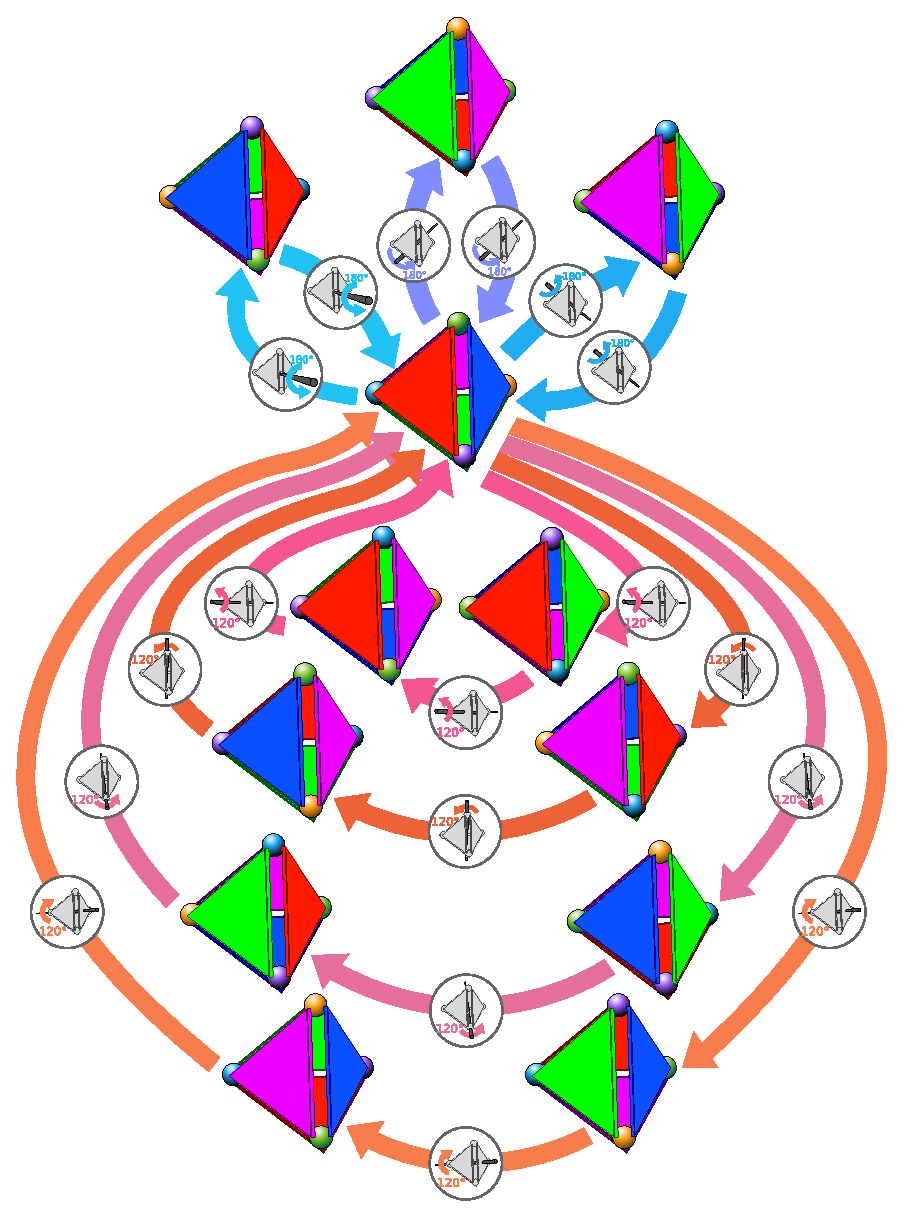
\includegraphics[scale=0.22]{figs/intro4}
\end{figure}
\end{frame}

\scriptsize

\opage{
\otitle{4.1 The angular momentum and their commutation relations}

% 4.1 skipped
\setcounter{equation}{1}

\otext
In classical mechanics, the \textit{angular momentum}, $l$, of a particle travelling with a linear momentum $p$ at a position $r$ on its path is defined as the vector product $l = r \times p$:

\begin{columns}

\begin{column}{4cm}
\ofig{angmom}{0.6}{}
\end{column}

\begin{column}{4cm}
The direction of the vector $l$ is given by the right-hand screw rule. It points perpendicular to the plane of rotation.
\end{column}

\end{columns}

If the position $r = xi + yj + zk$ and momentum $p = p_xi + p_yj + p_zk$ are multiplied out, we get:

\aeqn{4.2}{l = r\times p = (yp_z - zp_y)i + (zp_x - xp_z)j + (xp_y - yp_x)k}

where the components of $l$ can be identified:

\aeqn{4.3}{l_x = yp_z - zp_y\textnormal{, }l_y = zp_x - xp_z\textnormal{, }l_z = xp_y - yp_x}

The magnitude of the angular momentum is obtained through:

\aeqn{4.4}{l^2 = l_x^2 + l_y^2 + l_z^2}

}

\opage{

\otext
Transition to quantum mechanics can be carried out by replacing the classical observables by the corresponding operators:

\aeqn{4.5}{l_x = \frac{\hbar}{i}\left(y\frac{\partial}{\partial z} - z\frac{\partial}{\partial y}\right)\textnormal{, }l_y = \frac{\hbar}{i}\left(z\frac{\partial}{\partial x} - x\frac{\partial}{\partial z}\right)\textnormal{, }l_z = \frac{\hbar}{i}\left(x\frac{\partial}{\partial y} - y\frac{\partial}{\partial x}\right)}

The commutation relations between different Cartesian components of $l$ can be calculated as follows:

\beqn{4.6}{\hspace*{-1.4cm}\left[l_x,l_y\right] = \left[yp_z - zp_y, zp_x - xp_z\right] = \left[yp_z,zp_x\right] - \left[yp_z,xp_z\right] - \left[zp_y,zp_x\right] + \left[zp_y,xp_z\right]}
{y\left[p_z,z\right]p_x - 0 - 0 + xp_y\left[z,p_z\right] = i\hbar(-yp_x + xp_y) = i\hbar l_z}

Note that above, for example, $y$ and $p_x$ commute since they depend on different coordinates. In a similar way we can get the other commutators:

\aeqn{4.7}{\left[l_x,l_y\right] = i\hbar l_z\textnormal{, }\left[l_y,l_z\right] = i\hbar l_x\textnormal{, }\left[l_z,l_x\right] = i\hbar l_y}

For $l^2$ we have, since $\left[l^2_z, l_z\right] = 0$:

$$\left[l^2,l_z\right] = \left[l_x^2 + l_y^2 + l_z^2,l_z\right] = \left[l_x^2,l_z\right] + \left[l_y^2,l_z\right]$$

}

\opage{

\otext
For the other two commutators above we have:

$$\left[l_x^2,l_z\right] = L_xl_xl_z - l_zl_xl_x = l_xl_xl_z - l_xl_zl_x + l_xl_zl_x - l_zl_xl_x$$
$$= l_x\left[l_x,l_z\right] + \left[l_x,l_z\right]l_x = -i\hbar\left(l_xl_y + l_yl_x\right)$$

In a similar way we have:

$$\left[l^2_y,l_z\right] = i\hbar\left(l_xl_y + l_yl_x\right)$$

Since these are of equal magniture but opposite signs, they cancel out and we get:

\aeqn{4.8}{\left[l^2,l_q\right] = 0\textnormal{ where }q = x,y,z}

An observable is called an angular momentum if it follows the above commutation rules. It turns out that, for example, electron spin follows these rules and hence we say that it has angular momentum.

}

\opage{
\otitle{4.2 Definitions of additional thermodynamic potentials using Legendre transformations}

\otext
\textit{What is Legendre transformation?} Consider the following differential:

$$df(x,y) = \left(\frac{\partial f(x,y)}{\partial x}\right)dx + \left(\frac{\partial f(x,y)}{\partial y}\right)dy \equiv u(x,y)dx + v(x,y)dy$$

Change the differentials from ($dx$,$dy$) to ($du$,$dy$) with the following transformation:

$$g\equiv f - ux$$
$$dg = df - udx - xdu = udx + vdy - udx - xdu = vdy - xdu$$

\begin{columns}

\begin{column}{7cm}
where $x = -\frac{\partial g}{\partial u}$ and $v = \frac{\partial g}{\partial y}$. $x$ and $u$ are \textit{conjugate variables}.\\

\vspace*{0.2cm}

In a nutshell:\\

\vspace*{0.2cm}

``Transform the original differential in such a way that the new differential depends on the conjugate variables''

\vfill
\end{column}\vline\hspace*{0.1cm}

\begin{column}{3cm}
\operson{legendre}{0.6}{Adrien-Marie Legendre, French mathematician (1752 - 1833)}
\end{column}

\end{columns}

}

\opage{

\otext
Next, we will apply Legendre transformation to internal energy (ignore chemical potential for now):

\vspace*{-0.3cm}

$$d\umark{U}{``f\textnormal{''}} = \umark{-P}{``u\textnormal{''}}\umark{dV}{``dx\textnormal{''}} + \umark{T}{``v\textnormal{''}}\umark{dS}{``dy\textnormal{''}}$$
$$\umark{H}{``g\textnormal{''}} = \umark{U}{``f\textnormal{''}} - \umark{\left(-PV\right)}{``u\times x\textnormal{''}} = U + PV$$
$$\umark{dH}{``dg\textnormal{''}} = \umark{T}{``v\textnormal{''}}\umark{dS}{``dy\textnormal{''}} - \left(\umark{V}{``x\textnormal{''}}\times\umark{\left(-dP\right)}{``du\textnormal{''}}\right) = TdS + VdP$$

Now we have a new differential (enthalpy) $dH$ with new natural variables $S$ and $P$. Note that the original differential $dU$ had $S$ and $V$ as natural variables. Adding chemical potential does not change this result since we were not operating on the corresponding conjugate variables ($\mu_i$ and $n_i$):

\aeqn{4.20}{dH = TdS + VdP + \sum\limits_{i=1}^{N_s}\mu_i dn_i}

Recall that the total differential of $H$ is:

\vspace*{-0.4cm}

\aeqn{4.20a}{dH = \left(\frac{\partial H}{\partial S}\right)_{P,\lbrace n_i\rbrace} dS + \left(\frac{\partial H}{\partial P}\right)_{S,\lbrace n_i\rbrace} dP + \sum\limits_{i=1}^{N_s}\left(\frac{\partial H}{\partial n_i}\right)_{P,V,\lbrace n_j\rbrace_{j\ne i}} dn_i}

}

\opage{

\otext
By comparing the terms the same way as we did for $dU$, we get the following relations:

\aeqn{4.21}{T = \left(\frac{\partial H}{\partial S}\right)_{P,\lbrace n_i\rbrace}, V = \left(\frac{\partial H}{\partial P}\right)_{S,\lbrace n_i\rbrace},\mu_i = \left(\frac{\partial H}{\partial n_i}\right)_{S,P,\lbrace n_j\rbrace_{j\ne i}}}

Thus, if we can determine the partial derivatives of $H$ with respect to $S$, $P$ and $n_i$, we can always obtain $T$, $V$ and $\mu_i$ from Eq. (\ref{eq4.21}). A system under constant $S$, $P$, and $n_i$ combined with Eq. (\ref{eq4.20}) and exactly the same reasoning as in Eq. (\ref{eq4.17}) gives:

\aeqn{4.24}{\left(dH\right)_{S,P,\lbrace n_i\rbrace} \le 0}

A process occurs spontaneously at constant $S$, $P$ and $\lbrace n_i\rbrace$ if the enthalpy decreases.

\vspace*{0.2cm}

Furthermore, integration of Eq. (\ref{eq4.20}) under constant $T$, $P$ and $\lbrace \mu_i\rbrace$ results in:

\aeqn{4.25}{H = TS + \sum\limits_{i=1}^{N_s}\mu_i n_i}

Note that this yields Eq. (\ref{eq4.18}) when setting $H = U + PV$.

}

\opage{

\otext
Previously we established that $U$ and $H$ are connected to each other via Legendre transformation with conjugate variables $V$ and $P$. It is easier to control pressure than volume and therefore $H$ is more convenient to use in practice.

\vspace*{0.2cm}

How about the other conjugate variable pair ($T$, $S$)?

\vspace*{0.2cm}

Yes, it is more convenient to use temperature rather than entropy. Since ($V$, $P$) pair offers two choices ($U$ and $H$) and ($T$, $S$) another two, we have a total of four different possibilities:

\vspace*{0.2cm}

\begin{tabular}{llll}
Quantity & Natural variables & Energy & Differential (*)\\
Internal energy $U$ & $S, V, \lbrace n_i\rbrace$ &  $U$ & $dU = T dS - P dV$\\
Enthalpy $H$ & $S, P, \lbrace n_i\rbrace$ & $H = U + PV$ & $dH = T dS + V dP$\\
Helmholtz energy $A$ & $T, V, \lbrace n_i\rbrace$ & $A = U - TS$ & $dA = -S dT - P dV$\\
Gibbs energy $G$ & $T, P, \lbrace n_i\rbrace$ & $G = H - TS$ & $dG = -S dT + V dP$\\
\end{tabular}

\vspace*{0.2cm}

(*) chemical potential should be added to each differential. We are not considering Legendre transformation with respect to $n_i$ and $\mu_i$. The differential can also be derived from the given energy expression by considering the total differential.

\vspace*{0.2cm}

The last form is most useful in chemical applications since $T$ and $P$ can be controlled (i.e. they can be held constant).

}

\opage{

\begin{columns}

\begin{column}{7cm}

\otext
Expressions for the Helmholtz ``free energy'' ($A$):

\aeqn{4.29}{dA = -SdT - PdV + \sum\limits_{i=1}^{N_s} \mu_idn_i}

\aeqn{4.30}{S = -\left(\frac{\partial A}{\partial T}\right)_{V,\lbrace n_i\rbrace}}

\aeqn{4.31}{P = -\left(\frac{\partial A}{\partial V}\right)_{T,\lbrace n_i\rbrace}}

\aeqn{4.32}{\mu_i = \left(\frac{\partial A}{\partial n_i}\right)_{T,V,\lbrace n_j\rbrace_{j\ne i}}}

\aeqn{4.33}{\left(dA\right)_{T,V,\lbrace n_j\rbrace_{j\ne i}} \le 0}

\aeqn{4.34}{A = -PV + \sum\limits_{i = 1}^{N_s}\mu_i n_i}

\end{column}

\begin{column}{3cm}
\operson{helmholtz}{0.15}{Hermann von Helmholtz, German physicist (1821 - 1894)}
\end{column}

\end{columns}

\otext

At constant $T$, a change in the Helmholtz energy is given by $\Delta A = \Delta U - T\Delta S$. This gives the amount of internal energy that is ``free'' for doing work in a spontaneous process.

\vspace*{0.2cm}

\underline{Note:} Helmholtz energy is less useful in chemistry than the Gibbs energy because processes and reactions are more often carried out at constant pressure rather than constant volume.

}

\opage{

\otext
The corresponding expressions for the Gibbs energy ($G$) are:

\vspace*{-0.2cm}

\begin{columns}

\begin{column}{5cm}
\aeqn{4.36}{dG = -SdT + VdP + \sum\limits_{i=1}^{N_s}\mu_idn_i}
\aeqn{4.37}{S = -\left(\frac{\partial G}{\partial T}\right)_{P,\lbrace n_i\rbrace}}
\aeqn{4.38}{V = \left(\frac{\partial G}{\partial P}\right)_{T,\lbrace n_i\rbrace}}
\end{column}

\begin{column}{5cm}
\vspace*{0.8cm}
\aeqn{4.39}{\mu_i = \left(\frac{\partial G}{\partial n_i}\right)_{T,P,\lbrace n_i\rbrace}}
\vspace*{0.3cm}
\aeqn{4.44}{\left(dG\right)_{T,P,\lbrace n_i\rbrace}\le 0}
\vspace*{-0.1cm}
\aeqn{4.45}{G = \sum\limits_{i=1}^{N_s}\mu_in_i \textnormal{(const. }T,P,\mu_i\textnormal{)}}
\end{column}

\end{columns}


At constant $T$ and $P$, a change in the Gibbs energy is given by: $\Delta G = \Delta U + P\Delta V - T\Delta S$. In another words, it gives the maximum amount of internal energy that is available for doing non-expansion work in a spontaneous process.

\vspace*{0.2cm}

The related Maxwell equations (differentiation of the previous Eqs.):

\aeqn{4.46}{\left(\frac{\partial S}{\partial P}\right)_{T,\lbrace n_i\rbrace} = -\left(\frac{\partial^2 G}{\partial P\partial T}\right)_{T,\lbrace n_i\rbrace} = -\left(\frac{\partial^2 G}{\partial T\partial P}\right)_{P,\lbrace n_i\rbrace} = -\left(\frac{\partial V}{\partial T}\right)_{P,\lbrace n_i\rbrace}}

\aeqn{4.47}{\left(\frac{\partial S}{\partial n_i}\right)_{P,T,\lbrace n_j\rbrace_{j\ne i}} = -\left(\frac{\partial^2 G}{\partial n_i\partial T}\right)_{P,T,\lbrace n_j\rbrace_{j\ne i}} = -\left(\frac{\partial^2 G}{\partial T\partial n_i}\right)_{P,\lbrace n_i\rbrace} = -\left(\frac{\partial \mu_i}{\partial T}\right)_{P,\lbrace n_i\rbrace}}

}

\opage{

\otext

\aeqn{4.48}{\left(\frac{\partial V}{\partial n_i}\right)_{P,T,\lbrace n_j\rbrace_{j\ne i}} = \left(\frac{\partial^2 G}{\partial n_i\partial P}\right)_{P,T,\lbrace n_j\rbrace_{j\ne i}} = \left(\frac{\partial^2 G}{\partial P\partial n_i}\right)_{T,\lbrace n_i\rbrace} = \left(\frac{\partial \mu_i}{\partial P}\right)_{T,\lbrace n_i\rbrace}}

\underline{Note:} Since $G$ is a well behaving, the order of differentiation may changed.

\vspace*{0.2cm}

\textbf{Example.} Demonstrate the fact that if a thermodynamic potential is known as a function of its natural variables, we can calculate all of the thermodynamic properties of the system.

\vspace*{0.2cm}

\textbf{Solution.} We choose to show this for the Gibbs energy ($G$). So we assume that the value of $G$ is known as a function of its natural variables $(T, P, \lbrace n_i\rbrace)$. In this example we will consider only single species, so that the chemical potential sum vanishes. The entropy and volume of the system can be calculated using (Eqs. (\ref{eq4.37}) and (\ref{eq4.38})):

\vspace*{-0.4cm}

$$S = -\left(\frac{\partial G}{\partial T}\right)_P\textnormal{ and }V = \left(\frac{\partial G}{\partial P}\right)_T$$

Now using the equations given in the previous table, we have:

$$U = G - PV + TS = G - P\left(\frac{\partial G}{\partial P}\right)_T - T\left(\frac{\partial G}{\partial T}\right)_P$$

\vspace*{-0.3cm}

$$H = G + TS = G - T\left(\frac{\partial G}{\partial T}\right)_P\textnormal{ and }A = G - PV = G - P\left(\frac{\partial G}{\partial P}\right)_T$$

These expressions relate $U$, $H$, $A$, and $G$ to each other.

}

\opage{

\otext
\textbf{Example.} Show that the Gibbs energy gives a criterion for spontaneous change at constant $T = T_{sys} = T_{surr}$ and $P$.

\vspace*{0.2cm}

\textbf{Solution.} We need to show that $dG_{sys} \le 0 \Leftrightarrow dS_{tot} \ge 0$. First we calculate $dG_{sys}$ by noting that $G = H - TS$:

$$dG_{sys} = d\left(H_{sys} - TS_{sys}\right) = dH_{sys} - d\left(TS_{sys}\right) = dH_{sys} - \umark{S_{sys}dT}{=0} - TdS_{sys}$$
$$ = dq_{sys} - TdS_{sys} = -dq_{surr} - TdS_{sys} \le 0$$
$$\Leftrightarrow \umark{\frac{dq_{surr}}{T}}{=dS_{surr}} + dS_{sys} = dS_{tot} \ge 0$$

Thus for spontaneous (irreversible) changes, the Gibbs energy will always decrease with the equal sign applying only to reversible processes. Note that there is no need to consider the surroundings explicitly when predicting spontaneity using Gibbs energy whereas the calculation using entropy must consider both the system and surroundings explicitly.

\vspace*{0.2cm}

\underline{Note:} Although the above criteria show whether a certain change is spontaneous, it does not necessarily follow that the change will take place with an appreciable speed.

}

\opage{

\otext
When other than $PV$-work occurs in the system, it contributes a term to the fundamental equation for the internal energy (Eq. (\ref{eq2.40c})). They can be included in the Gibbs energy:

\aeqn{4.49}{dG = -SdT + VdP + \sum\limits_{i=1}^{N_s} \mu_idn_i + FdL + \gamma dA_S}

where $F$ is the force of extension, $L$ is the length, $\gamma$ is the surface tension and $A_S$ is the surface area. Variables ($F$ and $L$) and ($\gamma$ and $A_S$) are conjugate variables and:

\aeqn{4.50}{F = -\left(\frac{\partial G}{\partial L}\right)_{T,P,\lbrace n_i\rbrace,A_S}}

\aeqn{4.51}{\gamma = \left(\frac{\partial G}{\partial A_S}\right)_{T,P,\lbrace n_i\rbrace,L}}

What is the meaning of the Helmholtz and Gibbs energies in presence of non-$PV$ work?

\vspace*{0.2cm}

1. \textit{Helmholtz energy.} Consider the first law of thermodynamics (Eq. (\ref{eq2.9})): $dU = \inex{dq} + \inex{dw}$. Using Eq. (\ref{eq3.21}) gives:

\aeqn{4.53}{-dU + TdS \ge -\textnormal{ }\inex{dw}}

At constant temperature ($dT = 0$) we can write:

\aeqn{4.54}{-d\left(U - TS\right) \ge -\textnormal{ }\inex{dw}}

}

\opage{

\otext
This implies that:

\aeqn{4.55}{\left(dA\right)_T \le \inex{dw}}

where $A$ is the Helmholtz energy. Thus a change in the Helmholtz energy gives an upper bound for the work that can be done on the surroundings. In real processes the \textit{amount} work that can be done is less than $|\Delta A|$. In this case both sides of Eq. (\ref{eq4.55}) are negative ($dw < 0$ and $(dA)_T < 0$); i.e. when the system does work on the surroundings (i.e. $|(dA)_T| \ge |\inex{dw}|$).

\vspace*{0.2cm}

\underline{Note:} $\inex{dw}$ now contains both $PV$ and non-$PV$ work.

\vspace*{0.2cm}

2. \textit{Gibbs energy.} The Gibbs energy is especially useful when non-$PV$ work is involved. When $PV$ and non-$PV$ work are separated, the first law of thermodynamics (Eq. (\ref{eq2.9})) can be written:

\aeqn{4.56}{dU = \inex{dq} - P_{ext}dV + \inex{dw}_{nonPV}}

With the inequality (Eq. (\ref{eq3.21})) $TdS \ge \inex{dq}$ we can write:

\aeqn{4.57}{-dU - P_{ext}dV + TdS \ge -\inex{dw}_{nonPV}}

At constant $T$ and $P$ (= $P_{ext}$), we have:

\aeqn{4.58}{-d\left(U + PV - TS\right) \ge -\inex{dw}_{nonPV}}

\aeqn{4.59}{\left(dG\right)_{T,P} \le \inex{dw}_{nonPV}}

}

\opage{

\otext
\underline{Notes:}

\begin{enumerate}
\item For a reversible process at constant $T$ and $P$ the change in Gibbs energy is equal to the non-$PV$ work done on the system by the surroundings.\item Eq. (\ref{eq4.59}) states that a change in the Gibbs energy at constant $T$ and $P$ gives an upper bound for the non-$PV$ work that the system can do on its surroundings. \textit{Remember that in this case $dG$ and $dw_{nonPV}$ are negative.}
\item When work is done on the system, the Gibbs energy increases. When work is done by the system, the Gibbs energy decreases.
\end{enumerate}

\vfill

}

\opage{
\otitle{4.3 The reflection operation}

\otext
The reflection operation is denoted by $\sigma$ and the corresponding symmetry element is called a mirror plane. Given a symmetry plane, the $\sigma$ operation reflects each point to the opposite side of the plane. For example, some of the $\sigma$ symmetry elements in benzene are shown below.\\

\ofig{benzene4}{0.6}{Some of the $\sigma$ symmetry elements in benzene.}

\otext
$\sigma_d$ denotes a plane, which bisects the angle between the two $C_2$ axes and lies
parallel to the principal axis. The $\sigma_v$ plane includes the protons and the principal axis. The $\sigma_h$ is perpendicular to the principal axis. Note that two successive reflections $\sigma \sigma$ bring the molecule back to its original configuration (corresponding to an $E$ operation).

}

\opage{
\otitle{4.4 Effect of pressure on the Gibbs energy}

\otext
\underline{How does $G$ change as a function of pressure?}

\vspace*{0.2cm}

First Recall Eq. (\ref{eq4.38}): $\left(\frac{\partial G}{\partial P}\right)_{T,\lbrace n_i\rbrace} = V$. 

\vspace*{0.2cm}

Integration of this equation gives:

\aeqn{4.64}{\int\limits_{G_1}^{G_2} dG = \int\limits_{P_1}^{P_2}VdP \Rightarrow G_2 = G_1 + \int\limits_{P_1}^{P_2}\umark{V}{>0}dP}

Thus \textit{the Gibbs energy always increases with the increasing pressure} when $T$ and $\lbrace n_i\rbrace$
are constant.

\vspace*{0.2cm}

For liquids and solids volume ($V$) is approx. independent of pressure ($P$) and thus:

\aeqn{4.66}{G_2 = G_1 + V\left(P_2 - P_1\right)\textnormal{ or }\Delta G = V\Delta P}

For ideal gases ($PV = nRT$), we can write:

\aeqn{4.69}{G_2 = G_1 + nRT\ln\left(\frac{P_2}{P_1}\right)\textnormal{ or }\Delta G = nRT\ln\left(\frac{P_2}{P_1}\right)}

Setting $P_2 = P, P_1 = P^\circ, G_2 = G$ and $G_1 = G^\circ$, we get:

\aeqn{4.68}{G = G^\circ + nRT\ln\left(\frac{P}{P^\circ}\right)}

}

\opage{

\otext
\textbf{Example.} Given the expression for the molar Gibbs energy (Eq. (\ref{eq4.68})) and considering an ideal gas, derive the corresponding expression for the following thermodynamic properties: $V, U, H, S$ and $A$ at constant $T$.

\vspace*{0.2cm}

\textbf{Solution.} The molar Gibbs energy is given by Eq. (\ref{eq4.68}) with over bars:

$$\bar{G} = \bar{G}^\circ + RT\ln\left(\frac{P}{P^\circ}\right)$$

We need to find a similar -type expression for the above thermodynamic properties. The form should be: $X = X^\circ + \textnormal{``possible pressure correction''}$.
For an ideal gas we have:

$$P\bar{V} = RT \Rightarrow \bar{V} = \frac{RT}{P}$$


Based on Eq. (\ref{eq2.69}), the internal energy of an ideal gas does not depend on volume or pressure but only on temperature:

$$\bar{U} = \bar{U}^\circ$$

Recall that enthalpy is defined as $H = U + PV$. For an ideal gas $PV =$ constant $= nRT$, thus:

$$\bar{H} = \bar{U} + P\bar{V} = \bar{U}^\circ + RT = \bar{H}^\circ$$

}

\opage{

\otext
Eq. (\ref{eq3.36}) for the molar entropy states that: $\bar{S} = \bar{S}^\circ - R\ln\left(\frac{P}{P^\circ}\right)$.

\vspace*{0.2cm}

For the Helmholtz energy we have:

$$\bar{A}^\circ = \bar{G}^\circ - P\bar{V} = \bar{G}^\circ - RT$$
$$\Rightarrow \bar{A} = \bar{G} - P\bar{V} = \bar{G} - RT = \umark{\bar{G}^\circ - RT}{= \bar{A}^\circ} + RT\ln\left(\frac{P}{P^\circ}\right) = \bar{A}^\circ + RT\ln\left(\frac{P}{P^\circ}\right)$$

\vspace*{0.3cm}

\textbf{Example.} An ideal gas at 27 \degree C expands isothermally and reversibly from 10.00 to 1.000 bar against a pressure that is gradually reduced. Calculate $q$ per mole and $w$ per mole and each of the thermodynamic quantities $\Delta \bar{G}$, $\Delta \bar{U}$, $\Delta \bar{H}$, $\Delta \bar{S}$ and $\Delta \bar{A}$.

\vspace*{0.2cm}

\textbf{Solution.} Since the process is reversible \& isothermal and the gas is ideal, we have:

$$dw = -P_{ext}d\bar{V} = -Pd\bar{V} \Rightarrow w = -RT\ln\left(\frac{\bar{V}_2}{\bar{V}_1}\right) = -RT\ln\left(\frac{P_1}{P_2}\right)$$
$$= -\left(8.3145\textnormal{ J K}^{-1}\textnormal{ mol}^{-1}\right)\times\left(300.15\textnormal{ K}\right)\times\ln\left(\frac{10.00\textnormal{ bar}}{1.000\textnormal{ bar}}\right) = -5746\textnormal{ J mol}^{-1}$$

}

\opage{

\otext
Recall that Helmholtz energy gives the maximum amount of work that the system can do in a reversible process. Here the work and Helmholtz energy should be equal. Formally this can be seen integrating Eq. (\ref{eq4.29}) at constant $T$:

$$dA = -S\umark{dT}{\equiv 0} - PdV = -PdV = dw \Rightarrow \Delta \bar{A} = w = -5746\textnormal{ J mol}^{-1}$$

The internal energy of an ideal gas depends only on temperature and hence:

$$\Delta\bar{U} = 0 \Rightarrow q = \Delta\bar{U} - w = 5746\textnormal{ J mol}^{-1}$$

Likewise, the enthalpy of an ideal gas depends only on temperature:

$$\Delta\bar{H} = \Delta\bar{U} + \Delta\left(P\bar{V}\right) = \umark{\Delta\bar{U}}{\equiv 0} + \umark{\Delta\left(RT\right)}{\equiv 0} = 0$$

To get the change in the Gibbs energy ($\Delta\bar{G}$), we integrate Eq. (\ref{eq4.38}):

$$\Delta\bar{G} = \int\limits_{G_1}^{G_2} dG = \int\limits_{P_1}^{P_2} \bar{V}dP = \int\limits_{P_1}^{P_2}\frac{RT}{P}dP = RT\ln\left(\frac{P_2}{P_1}\right)$$
$$= \left(8.3145\textnormal{ J K}^{-1}\textnormal{ mol}^{-1}\right)\times\left(300.15\textnormal{ K}\right)\times\ln\left(\frac{1.000\textnormal{ bar}}{10.00\textnormal{ bar}}\right) = -5746\textnormal{ J mol}^{-1}$$

}

\opage{

\otext
Entropy for a reversible process at constant $T$ can be calculated using Eq. (\ref{eq3.9}):

$$\Delta\bar{S} = \frac{q_{rev}}{T} = \frac{5746\textnormal{ J mol}^{-1}}{300.15\textnormal{ K}} = 19.14\textnormal{ J K}^{-1}\textnormal{ mol}^{-1}$$

Another way to calculate the entropy difference is (``$G = H - TS$''):

$$\Delta\bar{S} = \frac{\Delta\bar{H} - \Delta\bar{G}}{T} = 19.14\textnormal{ J K}^{-1}\textnormal{ mol}^{-1}$$

\textbf{Example.} An ideal gas expands isothermally at 27 \degree C into an evacuated vessel so that the pressure drops from 10.00 to 1.000 bar; that is, it expands from a vessel of 2.463 L into a connecting vessel such that the total volume becomes 24.63 L. Calculate the change in thermodynamic quantities that were calculated in the previous example.

\vspace*{0.2cm}

\textbf{Solution.} This process is isothermal but NOT reversible. Since the system as a whole is closed, no external work is done and $w = 0$. Also at constant $T$, $\Delta U = 0$ and hence the first law of thermodynamics implies that also $q = 0$. The other quantities are the same as in the previous example, because the quantities are state functions and the choice of path does not affect the result. Both initial and final states in this example are identical to those in the previous example.

}

\opage{

\otext
\textbf{Example.} Calculate the Gibbs energy of formation at 10.00 bar and 298.15 K for: (a) Gaseous methanol (CH$_3$OH) (the standard Gibbs energy of formation $-161.96$ kJ mol$^{-1}$) and (b) Liquid methanol (density 0.7914 g cm$^{-3}$ and the standard Gibbs energy of formation $-166.27$ kJ mol$^{-1}$). Assume that gaseous methanol behaves according to the ideal gas law.

\vspace*{0.2cm}

\textbf{Solution.} The Gibbs energy of formation is defined essentially the same way as we defined the enthalpy of formation previously. For (a) we can use Eq. (\ref{eq4.68}):

$$\Delta_f G = \Delta_f G^\circ + RT\ln\left(\frac{P}{P^\circ}\right) = -161.96\textnormal{ kJ mol}^{-1} + \left(8.3145\times 10^{-3}\textnormal{ kJ K}^{-1}\textnormal{ mol}^{-1}\right)$$
$$\times\left(298.15\textnormal{ K}\right)\times\ln\left(\frac{10.00\textnormal{ bar}}{1.000\textnormal{ bar}}\right) = -156.25\textnormal{ kJ mol}^{-1}$$

Thus we see that the Gibbs energy of formation is higher at higher pressure. In practice this means that it was not as favorable to form methanol at high pressure than at the low pressure. In both cases the reaction is spontaneous.

\vspace*{0.2cm}

For (b) the molar volume of the liquid is approximately independent of pressure.
In this case we can use directly Eq. (\ref{eq4.66}). First we have to calculate to molar volume:

}

\opage{

\otext
$$\bar{V} = \frac{M_{\textnormal{CH}_3\textnormal{OH}}}{\rho_{\textnormal{CH}_3\textnormal{OH}}} = \frac{32.04\textnormal{ g mol}^{-1}}{0.7914\textnormal{ g cm}^{-3}} = 40.49 \textnormal{ cm}^3\textnormal{ mol}^{-1}$$
$$= \left(40.49\textnormal{ cm}^3\textnormal{ mol}^{-1}\right)\times\left(10^{-2}\textnormal{ m cm}^{-1}\right)^3 = 40.49\times 10^{-6}\textnormal{ m}^3\textnormal{ mol}^{-1}$$

This gives the molar Gibbs energy of formation:
$$\Delta_f G = \Delta_f G^\circ + \bar{V}\left(P - P^\circ\right) = \left(-166.27\textnormal{ kJ mol}^{-1}\right) + \left(40.49\times 10^{-6}\textnormal{ m}^3\textnormal{ mol}^{-1}\right)$$
$$\times \left(\frac{9\times 10^5\textnormal{ Pa}}{10^3\textnormal{J / kJ}}\right) = -166.23\textnormal{ kJ mol}^{-1}$$

\vspace*{-0.8cm}

\begin{columns}

\begin{column}{5cm}
\otext

\underline{Note:} The Gibbs energy of formation for a gases and liquids have very different pressure dependency. This can be seen in the graph shown on the right (the value of the $\bar{V}\times\Delta P$ term above for the liquid is small compared to $\Delta_f G^\circ$). At the intersection, both species have the same molar volume.

\end{column}

\vspace*{-0.2cm}

\begin{column}{4cm}

\ofig{gibbs-liquid-gas}{0.25}{}

\end{column}

\end{columns}

}

\opage{
\otitle{4.5 Rotation-reflection operation}

\otext
Rotation-reflection operation is denoted by $S_n$. It consists of two different operations: $C_n$ and $\sigma_h$, which are executed in sequence. Note that a molecule may not necessary possess a proper symmetry with respect to these individual operations but may still have the overall $S_n$ symmetry. For example, benzene has $S_6$ symmetry as well as $C_6$ and $\sigma_h$ whereas a tetrahedral CH$_4$ has $S_4$ but not $C_4$ or $\sigma_h$ alone:

\ofig{methane}{0.55}{$S_4$ symmetry operation in methane. Note that the symmetry is temporarily lost after $C_4$.}

\vspace{0.5cm}
It can be shown that $(S_4)^2 = C_2$ and $(S_4)^4 = E$.

}

\opage{
\otitle{4.6 Identification of point groups of molecules}

\otext
A given molecule may have a number of possible symmetry operations. These symmetry operations form a mathematical group if they satisfy the following requirements:\\

\begin{enumerate}
\item If two symmetry operations are ``multiplied'' together (i.e. they are applied in sequence), the resulting overall symmetry operation must also belong to the group.\\
\item The group must always contain the identity operation ($E$).\\
\item The symmetry operations in a group must be associative: $(AB)C = A(BC)$. Note that they do not have to commute (e.g. it may be that $AB \ne BA$).\\
\item Each symmetry operation must have an inverse operation: for symmetry operation $A$ there must be another symmetry operation $A^{-1}$ for which $AA^{-1} = E$.\\
\end{enumerate}
\vspace{-0.5cm}
\begin{columns}
\begin{column}{5cm}

\otext
A group is called \textbf{Abelian} if the multiplication operation is commutative (i.e. $AB = BA$). If this does not hold, the group is \textbf{non-Abelian}.

\end{column}
\begin{column}{4cm}
\operson{Niels_Henrik_Abel}{0.08}{Niels Henrik Abel (1802 - 1829) Norwegian mathematician.}
\end{column}
\end{columns}

}

\opage{

\otext
The groups of symmetry operations for molecules are called \textbf{point groups} because one spatial point is left unchanged by every symmetry operation. Note that this point is not necessarily occupied by any nucleus. The \textbf{Schoenflies notation} is typically used in quantum mechanics and spectroscopy whereas the \textbf{Hermann-Maunguin notation} is used in crystallography. In the following, we will concentrate on the Schoenflies notation. A list of point groups and the corresponding symmetry operations are given below.

\ofig{sym1}{0.5}{}

}

\opage{

\ofig{sym2}{0.5}{}

}

\opage{

\ofig{sym3}{0.5}{}

\otext
\underline{Notes:}\\
\begin{itemize}
\item Linear molecules are always either $C_{\infty v}$ or $D_{\infty h}$.
\item Point groups $C_{\infty v}$, $D_{\infty h}$, $T_d$ and $O_h$ are sometimes called \textbf{special groups}.
\item Short notation, for example: $2C_3$ indicates that there are two ``similar'' $C_3$ operations (for example, the $+$/$-$ pairs).
\end{itemize}

}

\opage{
\otext
Determination of the point group for a given molecule can be a tedious task. Therefore it is helpful to use the following flowchart for determining the point group:

\ofig{flowchart}{0.3}{}

}

\opage{
\otitle{4.7 Symmetry, polarity and chirality}

\otext
A \textbf{polar molecule} has a permanent dipole moment. Examples of polar molecules are HCl, O$_3$ and NH$_3$. If a molecule belongs to $C_n$ group with $n > 1$, it cannot possess a charge distribution with a dipole moment perpendicular to the symmetry axis. Any dipole that exists in one direction perpendicular to the axis is cancelled by an opposing dipole from the other side. For example, in H$_2$O the perpendicular component of the dipole associated with one OH bond is cancelled by an equal but opposite component of the dipole of the second OH bond. Thus the dipole moment must be oriented along the $C_2$ axis of water:

\ofig{water}{0.6}{The total dipole moment in water is a vector sum from the polar bonds.}

}

\opage{

\otext
The same reasoning applies to molecules having $C_{nv}$ symmetry and they may be polar. In all other groups, such as $C_{3h}$, $D$, etc., there are symmetry operations that take one end of the molecule into the other. Therefore these molecules may not have permanent dipole moment along any axis. In general, only molecules belonging to the groups $C_n$, $C_{nv}$ and $C_s$ may have a permanent dipole moment. For $C_n$ and $C_{nv}$ the dipole moment lies along the symmetry axis. For example, O$_3$ (ozone), which is nonlinear and belongs to $C_{2v}$, may be polar (and is). On the other hand, CO$_2$, which is linear and belongs to $D_{\infty h}$, is not polar.

\otext
A \textbf{chiral molecule} is a molecule that cannot be superimposed on its mirror image. Chiral molecules are optically active in the sense that they rotate the plane of polarized light. A chiral molecule and its mirror-image partner constitute an \textbf{enantiomeric pair} of isomers and rotate the plane of polarization in equal amounts but in opposite directions.

\otext
According to the theory of optical activity, a molecule \underline{may} be chiral only if it does not possess an axis of improper rotation ($S_n$; ``converts a left-handed molecule into a right-handed molecule''). Note that such an axis may be present implicitly as, for example, $C_{nh}$ has an $S_n$ axis (combined $C_n$ and $\sigma_h$). Also, any molecule that has a center of inversion ($i$) has an $S_2$ axis (combined $C_2$ and $\sigma_h$). Thus any molecule with centers of inversion are \textbf{achiral} (not chiral). Because $S_1 = \sigma$ any molecule with a mirror plane is achiral. Note that a molecule may be achiral eventhough it does not have a center of inversion. Thermal motion may also
result in fast conversion between the isomers quenching the optical activity.

}

\opage{

\otext
\textbf{Example.} Is H$_2$O$_2$ chiral?\\
\textbf{Solution.} H$_2$O$_2$ has two isomers:\\

\ofig{h2o2}{0.8}{Two isomers of H$_2$O$_2$ with the $C_2$ symmetry axes (along the plane and out of plane) are shown.}

\otext
This molecule has no explicit or implicit $S_n$ axes and therefore it may be chiral. In fact, it is known to be chiral at low temperatures where the interconversion between the two isomers is forbidden. Equal populations of the isomers give a solution that is achiral overall (\textit{rasemic}).

}
% TODO: check above that rasemic is the right term

\opage{
\otitle{4.8 Matrix representation of symmetry operations}

\otext
Symmetry operations can be written as matrices, which transform the object accordingly in space. In case of rotation, these are called \textbf{rotation matrices}. Consider first the inversion ($i$) operation, which we have seen to map coordinates $(x_1, y_1, z_1)$
to $(x_2, y_2, z_2)$ where $x_1 = -x_2, y_1 = -y_2, z_1 = -z_2$. This can be written in matrix form as follows:

\aeqn{12.4}{
\begin{pmatrix}
x_2\\
y_2\\
z_2\\
\end{pmatrix}
=
\begin{pmatrix}
-1 & 0 & 0\\
0 & -1 & 0\\
0 & 0 & -1\\
\end{pmatrix}
\begin{pmatrix}
x_1\\
y_1\\
z_1\\
\end{pmatrix}
=
\begin{pmatrix}
-x_1\\
-y_1\\
-z_1\\
\end{pmatrix}
}

\otext
Now we can identify the matrix that corresponds to $i$ as:\vspace{0.5cm}

\aeqn{12.5}{
D(i) = 
\begin{pmatrix}
-1 & 0 & 0\\
0 & -1 & 0\\
0 & 0 & -1\\
\end{pmatrix}
}

\otext
The identity operation ($E$) is clearly then:\vspace{0.5cm}

\aeqn{12.6}{
D(E) = 
\begin{pmatrix}
1 & 0 & 0\\
0 & 1 & 0\\
0 & 0 & 1\\
\end{pmatrix}
}

}

\opage{

\otext
In general, \textbf{the matrix representation depends on the basis set and the choice of coordinate system}. In the following, we consider three atomic $p_x$ orbitals in SO$_2$ molecule:

\ofig{so2}{1.25}{Atomic $p_x$ orbitals in SO$_2$ ($C_{2v}$). Consider the orbitals as free atomic orbitals in this example.}

\otext
Denote the $p_x$ orbitals on O atoms labeled as A and B by $p_A$ and $p_B$, respectively. The $p_x$ orbital of S atom is denoted by $p_S$. Consider first a $\sigma_v$ operation, which transforms $(p_S, p_A, p_B) \rightarrow (p_S, p_B, p_A)$. This can be written in matrix form as follows:

\aeqn{12.7}{
\begin{pmatrix}
p_S\\
p_B\\
p_A\\
\end{pmatrix}
=
\begin{pmatrix}
1 & 0 & 0\\
0 & 0 & 1\\
0 & 1 & 0\\
\end{pmatrix}
\begin{pmatrix}
p_S\\
p_A\\
p_B\\
\end{pmatrix}
}

}

\opage{

\otext
Thus the \textbf{matrix representative} of $\sigma_v(xz)$ in this case is:

\aeqn{12.8}{
D(\sigma_v) = 
\begin{pmatrix}
1 & 0 & 0\\
0 & 0 & 1\\
0 & 1 & 0\\
\end{pmatrix}
}
\vspace{-0.25cm}

\otext
The same method can be used to find matrix representatives for the other symmetry operations in $C_{2v}$. The effect of $C_2$ is to map $(p_S, p_A, p_B) \rightarrow (-p_S, -p_B, -p_A)$ and its representative is:

\aeqn{12.9}{
D(C_2) = 
\begin{pmatrix}
-1 & 0 & 0\\
0 & 0 & -1\\
0 & -1 & 0\\
\end{pmatrix}
}

\otext
The effect of $\sigma_v'(yz)$ is $(p_S, p_A, p_B) \rightarrow (-p_S, -p_A, -p_B)$ and the representative is:

\aeqn{12.10}{
D(\sigma_v') = 
\begin{pmatrix}
-1 & 0 & 0\\
0 & -1 & 0\\
0 & 0 & -1\\
\end{pmatrix}
}
\vspace{-0.25cm}

\otext
The identity operation ($E$) has no effect on the $p$ orbitals and therefore it corresponds to a unit matrix:

\aeqn{12.11}{
D(E) = 
\begin{pmatrix}
1 & 0 & 0\\
0 & 1 & 0\\
0 & 0 & 1\\
\end{pmatrix}
}

}

\opage{

\otext
The set of matrices that represents all the operations of the group is called a \textbf{matrix representation} (denoted by $\Gamma$). The dimension of the basis set (above 3 - the three $p_x$ orbitals) is denoted by a superscript, $\Gamma^{(3)}$.

\otext
The \textbf{character} of an operation in a given representation ($\chi$) is the sum of the diagonal elements of its matrix representative (matrix trace denoted by Tr()). The character of an operation depends on the basis set used. For example, the characters of previously found matrix representations are:
\vspace{-0.25cm}

\deqn{12.12}{\chi(E) \equiv \textnormal{Tr}(E) = 1 + 1 + 1 = 3}
{\chi(C_2)\equiv\textnormal{Tr}(C_2) = -1 + 0 + 0 = -1}
{\chi(\sigma_v(xz))\equiv\textnormal{Tr}(\sigma_v(xz)) = 1 + 0 + 0 = 1}
{\chi(\sigma_v'(yz))\equiv\textnormal{Tr}(\sigma_v'(yz)) = -1 - 1 - 1 = -3}

\vspace{-0.25cm}

\otext
The previous matrix representatives appear to be in \textbf{block diagonal form}:

\aeqn{12.13}{D =
\begin{pmatrix}
X & 0 & 0\\
0 & X & X\\
0 & X & X\\
\end{pmatrix}
}

Thus the symmetry operations in $C_{2v}$ do not mix $p_S$ with $p_A$ and $p_B$ basis functions. This suggests that the matrix representation $\Gamma^{(3)}$ can be decomposed into two independent matrix representations (one for $p_S$ and one for $p_A$ and $p_B$).

}

\opage{

\otext
For $p_S$ we get (parentheses signify that these are matrices in general):

\deqn{12.14}{D(E) = (1)}{D(C_2) = (-1)}{D(\sigma_v) = (1)}{D(\sigma_v') = (-1)}

This one dimensional matrix representation is now denoted by $\Gamma^{(1)}$. For the $p_A$ and $p_B$, the matrix representation is found to be:

\deqn{12.15}{
D(E) = \begin{pmatrix}
1 & 0\\
0 & 1\\
\end{pmatrix}
}
{
D(\sigma_v) = \begin{pmatrix}
0 & 1\\
1 & 0\\
\end{pmatrix}
}
{
D(C_2) = \begin{pmatrix}
0 & -1\\
-1 & 0\\
\end{pmatrix}
}
{
D(\sigma_v') = \begin{pmatrix}
-1 & 0\\
0 & -1\\
\end{pmatrix}
}

\vspace{-0.5cm}

\otext
This is denoted by $\Gamma^{(2)}$.

}

\opage{

\otext
The relationship between the original matrix representation and the above two reduced representations is written symbolically as:

\aeqn{12.16}{\Gamma^{(3)} = \Gamma^{(1)} + \Gamma^{(2)}}

Clearly the one-dimensional matrix representation $\Gamma^{(1)}$ cannot be reduced any further. A matrix representation that cannot reduced any further is called an \textbf{irreducuble representation} (or irrep for short).

\otext
How about the two-dimensional $\Gamma^{(2)}$? The matrices are not in block diagonal form and no further reduction is possible in this basis set. However, if we would choose our basis set slightly differently:

\vspace{-0.25cm}

\beqn{12.17}{p_1 = p_A + p_B}{p_2 = p_A - p_B}

\vspace{-1cm}

\ofig{so2a}{1.25}{$p_1$ and $p_2$ basis functions in SO$_2$.}

}

\opage{

\otext
In this new basis set the matrix representations in $\Gamma^{(2)}$ can be written as (``how does $(p_1, p_2)$ transform?''):

\deqn{12.18}{
D(E) = 
\begin{pmatrix}
1 & 0\\
0 & 1\\
\end{pmatrix}
}
{
D(\sigma_v) =
\begin{pmatrix}
1 & 0\\
0 & -1\\
\end{pmatrix}
}
{
D(C_2) =
\begin{pmatrix}
-1 & 0\\
0 & 1\\
\end{pmatrix}
}
{
D(\sigma_v') =
\begin{pmatrix}
-1 & 0\\
0 & -1\\
\end{pmatrix}
}

\otext
These matrices are in block diagonal form and therefore we can break the above representation into two one-dimensional representations. $p_1$ spans (identical to $\Gamma^{(1)}$ for $p_S$):

\deqn{12.19}{D(E) = (1)}{D(C_2) = (-1)}{D(\sigma_v) = (1)}{D(\sigma_v') = (-1)}

}

\opage{

\otext
and $p_2$ spans (denoted by $\Gamma^{(1)'}$):

\deqn{12.20}{D(E) = (1)}{D(C_2) = (1)}{D(\sigma_v) = (-1)}{D(\sigma_v') = (-1)}

\otext
In $C_{2v}$ the irreducible representation (irrep) corresponding to $\Gamma^{(1)}$ above is denoted by $B_1$ and $\Gamma^{(1)'}$ is denoted by $A_2$. What irreps would arise from an oxygen $s$-atom orbital basis?

\otext
In general, $C_{2v}$ can can have four kinds of irreps each with its own unique set of characters (ignore the Modes and Operators columns for now) as shown in the $C_{2v}$ character table.

\begin{table}
\caption{Character table for $C_1$ point group (Abelian, possibly chiral).}
\begin{tabular}{l|@{\extracolsep{1.5cm}}r@{\extracolsep{1.5cm}}l@{\extracolsep{1.5cm}}l}
$C_1$ & $E$ & Modes & Operators\\
\hline
$A$ & 1 & $R_x, R_y, R_z, T_x, T_y, T_z$ & $x, y, z, ...$\\
\end{tabular}
\end{table}

}

\opage{

\begin{table}
\caption{Character table for $C_s = C_h$ point group (Abelian, achiral).}
\begin{tabular}{l|@{\extracolsep{1cm}}r@{\extracolsep{1cm}}r@{\extracolsep{1cm}}l@{\extracolsep{1cm}}l}
$C_s$ & $E$ & $\sigma_h$ & Modes & Operators\\
\hline
$A'$ & 1 & 1 & $R_z, T_x, T_y$ & $x, y, x^2, y^2, z^2, xy$\\
$A''$ & 1 & $-1$ & $R_x, R_y, T_z$ & $z, yz, xz$\\
\end{tabular}
\end{table}

\begin{table}
\caption{Character table for $C_i = S_2$ point group (Abelian, achiral).}
\begin{tabular}{l|@{\extracolsep{1cm}}r@{\extracolsep{1cm}}r@{\extracolsep{1cm}}l@{\extracolsep{1cm}}l}
$C_i$ & $E$ & $i$ & Modes & Operators\\
\hline
$A_g$ & 1 & 1 & $R_x, R_y, R_z$ & $x^2, y^2, z^2, xy, xz, yz$\\
$A_u$ & 1 & $-1$ & $T_x, T_y, T_z$ & $x, y, z$\\
\end{tabular}
\end{table}

\begin{table}
\caption{Character table for $C_{2v}$ point group (Abelian, achiral).}
\begin{tabular}{l|@{\extracolsep{0.7cm}}r@{\extracolsep{0.7cm}}r@{\extracolsep{0.7cm}}r@{\extracolsep{0.7cm}}r@{\extracolsep{0.7cm}}l@{\extracolsep{0.7cm}}l}
$C_{2v}$ & $E$ & $C_2$ & $\sigma_v (xz)$ & $\sigma_v '(yz)$ & Modes & Operators \\
\hline
$A_1$ & 1 & 1 & 1 & 1 & $T_z$ & $z, x^2, y^2, z^2$ \\
$A_2$ & 1 & 1 & $-1$ & $-1$ & $R_z$ & $xy$ \\
$B_1$ & 1 & $-1$ & 1 & $-1$ & $T_{x}, R_{y}$ & $x, xz$ \\
$B_2$ & 1 & $-1$ & $-1$ & 1 & $T_{y}, R_{x}$ & $y, yz$ \\
\end{tabular}
\end{table}

}

\opage{

\begin{table}
\caption{Character table for $C_{3v}$ point group (non-Abelian, achiral).}
\begin{tabular}{l|@{\extracolsep{0.5cm}}r@{\extracolsep{0.5cm}}r@{\extracolsep{0.5cm}}r@{\extracolsep{0.5cm}}l@{\extracolsep{0.5cm}}l}
$C_{3v}$ & $E$ & $2C_3$ & $3\sigma_v$ & Modes & Operators \\
\hline
$A_1$ & 1 & 1 & 1 & $T_z$ & $z, x^2 + y^2, z^2$ \\
$A_2$ & 1 & 1 & $-1$ & $R_z$ & \\
$E$ & 2 & $-1$ & 0 & $T_{x}, T_{y}, R_{x}, R_{y}$ & $x, y, x^2 - y^2, xy, xz, yz$ \\
\end{tabular}
\end{table}

\begin{table}
\caption{Character table for $C_{4v}$ point group (non-Abelian, achiral).\hfill}
\begin{tabular}{l|@{\extracolsep{0.4cm}}r@{\extracolsep{0.4cm}}r@{\extracolsep{0.4cm}}r@{\extracolsep{0.4cm}}r@{\extracolsep{0.4cm}}r@{\extracolsep{0.4cm}}l@{\extracolsep{0.4cm}}l}
$C_{4v}$ & $E$ & $C_2$ & $2C_4$ & $2\sigma_v$ & $2\sigma_d$ & Modes & Operators\\
\hline
$A_1$ & 1 & 1 & 1 & 1 & 1 & $T_z$ & $z, x^2 + y^2, z^2$\\
$A_2$ & 1 & 1 & 1 & $-1$ & $-1$ & $R_z$ & \\
$B_1$ & 1 & 1 & $-1$ & 1 & $-1$ & & $x^2 - y^2$\\
$B_2$ & 1 & 1 & $-1$ & $-1$ & 1 & & $xy$\\
$E$ & 2 & $-2$ & 0 & 0 & 0 & $T_x, T_y, R_x, R_y$ & $x, y, xz, yz$\\
\end{tabular}
\end{table}

}

\opage{

\begin{table}
\caption{Character table for $C_{5v}$ point group (non-Abelian, achiral, $\alpha = 2\pi/5$).}
\begin{tabular}{l|@{\extracolsep{0.4cm}}r@{\extracolsep{0.4cm}}r@{\extracolsep{0.4cm}}r@{\extracolsep{0.4cm}}r@{\extracolsep{0.4cm}}l@{\extracolsep{0.4cm}}l}
$C_{5v}$ & $E$ & $2C_5$ & $2C_5^2$ & $5\sigma_v$ & Modes & Operators \\
\hline
$A_1$ & 1 & 1 & 1 & 1 & $T_z$ & $z, x^2 + y^2, z^2$ \\
$A_2$ & 1 & 1 & 1 & $-1$ & $R_z$ & \\
$E_1$ & 2 & $2$cos$(\alpha)$ & $2$cos$(2\alpha)$ & 0 & $R_x, R_y, T_x, T_y$ & $x, y, xz, yz$ \\
$E_2$ & 2 & $2$cos$(2\alpha)$ & $2$cos$(\alpha)$ & 0 & & $xy, x^2 - y^2$ \\
\end{tabular}
\end{table}

\begin{table}
\caption{Character table for $C_{6v}$ point group (non-Abelian, achiral).}
\begin{tabular}{l|@{\extracolsep{0.3cm}}r@{\extracolsep{0.3cm}}r@{\extracolsep{0.3cm}}r@{\extracolsep{0.3cm}}r@{\extracolsep{0.3cm}}r@{\extracolsep{0.3cm}}r@{\extracolsep{0.3cm}}l@{\extracolsep{0.3cm}}l}
$C_{6v}$ & $E$ & $C_2$ & $2C_3$ & $2C_6$ & $3\sigma_d$ & $3\sigma_v$ & Modes & Operators \\
\hline
$A_1$ & 1 & 1 & 1 & 1 & 1 & 1 & $T_z$ & $z, x^2 + y^2, z^2$ \\
$A_2$ & 1 & 1 & 1 & 1 & $-1$ & $-1$ & $R_z$ & \\
$B_1$ & 1 & $-1$ & 1 & $-1$ & $-1$ & 1 &  & \\
$B_2$ & 1 & $-1$ & 1 & $-1$ & 1 & $-1$ & & \\
$E_1$ & 2 & $-2$ & $-1$ & 1 & 0 & 0 & $R_x, R_y, T_x, T_y$ & $x, y, xz, yz$ \\
$E_2$ & 2 & 2 & $-1$ & $-1$ & 0 & 0 & & $xy, x^2 - y^2$ \\
\end{tabular}
\end{table}

}

\opage{

\begin{table}
\caption{Character table for $C_{\infty v}$ point group (non-Abelian, achiral). When $\phi = \pi$ only one member in $C_\phi$.}
\begin{tabular}{l|@{\extracolsep{0.5cm}}r@{\extracolsep{0.5cm}}r@{\extracolsep{0.5cm}}r@{\extracolsep{0.5cm}}r@{\extracolsep{0.5cm}}l@{\extracolsep{0.5cm}}l}
$C_{\infty v}$ & $E$ & $2C_\phi$ & ... & $\infty\sigma_v$ & Modes & Operators \\
\hline
$A_1 = \Sigma^+$ & 1 & 1 & ... & 1 & $T_z$ & $z, x^2 + y^2, z^2$ \\
$A_2 = \Sigma^-$ & 1 & 1 & ... & $-1$ & $R_z$ & \\
$E_1 = \Pi$ & 2 & $2\textnormal{cos}(\phi)$ & ... & 0 & $T_x, T_y, R_x, R_y$ & $x, y, xz, yz$ \\
$E_2 = \Delta$ & 2 & $2\textnormal{cos}(2\phi)$ & ... & 0 & & $x^2 - y^2, xy$ \\
$E_3 = \Phi$ & 2 & $2\textnormal{cos}(3\phi)$ & ... & 0 & & \\
... & ... & ... & ... & ... & & \\
\end{tabular}
\end{table}

\begin{table}
\caption{Character table for $D_2$ point group (Abelian, possibly chiral).}
\begin{tabular}{l|@{\extracolsep{0.4cm}}r@{\extracolsep{0.4cm}}r@{\extracolsep{0.4cm}}r@{\extracolsep{0.4cm}}r@{\extracolsep{0.4cm}}l@{\extracolsep{0.4cm}}l}
$D_2$ & $E$ & $C_2(z)$ & $C_2(y)$ & $C_2(x)$ & Modes & Operators \\
\hline
$A_1$ & 1 & 1 & 1 & 1 & & $x^2, y^2, z^2$ \\
$B_1$ & 1 & 1 & $-1$ & $-1$ & $R_z, T_z$ & $z, xy$ \\
$B_2$ & 1 & $-1$ & 1 & $-1$ & $R_y, T_y$ & $y, xz$ \\
$B_3$ & 1 & $-1$ & $-1$ & 1 & $R_x, T_x$ & $x,yz$ \\
\end{tabular}
\end{table}

}

\opage{

\begin{table}
\caption{Character table for $D_{2h}$ point group (Abelian, achiral).\hfill}
\begin{tabular}{l|@{\extracolsep{0.2cm}}r@{\extracolsep{0.2cm}}r@{\extracolsep{0.2cm}}r@{\extracolsep{0.2cm}}r@{\extracolsep{0.2cm}}r@{\extracolsep{0.2cm}}r@{\extracolsep{0.2cm}}r@{\extracolsep{0.2cm}}r@{\extracolsep{0.2cm}}l@{\extracolsep{0.2cm}}l}
$D_{2h}$ & $E$ & $C_2(z)$ & $C_2(y)$ & $C_2(x)$ & $i$ & $\sigma(xy)$ & $\sigma(xz)$ & $\sigma(yz)$ & Modes & Operators \\
\hline
$A_g$ & 1 & 1 & 1 & 1 & 1 & 1 & 1 & 1 & & $x^2, y^2, z^2$\\
$B_{1g}$ & 1 & 1 & $-1$ & $-1$ & 1 & 1 & $-1$ & $-1$ & $R_z$ & $xy$\\
$B_{2g}$ & 1 & $-1$ & 1 & $-1$ & 1 & $-1$ & 1 & $-1$ & $R_y$ & $xz$\\
$B_{3g}$ & 1 & $-1$ & $-1$ & 1 & 1 & $-1$ & $-1$ & 1 & $R_x$ & $yz$\\
$A_u$ & 1 & 1 & 1 & 1 & $-1$ & $-1$ & $-1$ & $-1$ & & \\
$B_{1u}$ & 1 & 1 & $-1$ & $-1$ & $-1$ & $-1$ & 1 & 1 & $T_z$ & $z$\\
$B_{2u}$ & 1 & $-1$ & 1 & $-1$ & $-1$ & 1 & $-1$ & 1 & $T_y$ & $y$\\
$B_{3u}$ & 1 & $-1$ & $-1$ & 1 & $-1$ & 1 & 1 & $-1$ & $T_x$ & $x$\\
\end{tabular}
\end{table}

\begin{table}
\caption{Character table for $D_{2d}$ point group (non-Abelian, achiral).\hfill}
\begin{tabular}{l|@{\extracolsep{0.4cm}}r@{\extracolsep{0.4cm}}r@{\extracolsep{0.4cm}}r@{\extracolsep{0.4cm}}r@{\extracolsep{0.4cm}}r@{\extracolsep{0.4cm}}l@{\extracolsep{0.4cm}}l}
$D_{2d}$ & $E$ & $2S_4$ & $C_2$ & $2C_2'$ & $2\sigma_d$ & Modes & Operators\\
\hline
$A_1$ & 1 & 1 & 1 & 1 & 1 & & $x^2 + y^2, z^2$\\
$A_2$ & 1 & 1 & 1 & $-1$ & $-1$ & $R_z$ & \\
$B_1$ & 1 & $-1$ & 1 & 1 & $-1$ & & $x^2 - y^2$\\
$B_2$ & 1 & $-1$ & 1 & $-1$ & 1 & $T_z$ & $z, xy$\\
$E$ & 2 & 0 & $-2$ & 0 & 0 & $T_x, T_y, R_x, R_y$ & $x, y, xz, yz$\\
\end{tabular}
\end{table}

}

\opage{

\begin{table}
\caption{Character table for $D_{3}$ point group (non-Abelian, possibly chiral).}
\begin{tabular}{l|@{\extracolsep{0.5cm}}r@{\extracolsep{0.5cm}}r@{\extracolsep{0.5cm}}r@{\extracolsep{0.5cm}}l@{\extracolsep{0.5cm}}l}
$D_3$ & $E$ & $2C_3$ & $3C_2'$ & Modes & Operators \\
\hline
$A_1$ & 1 & 1 & 1 & & $z^2, x^2 + y^2$ \\
$A_2$ & 1 & 1 & $-1$ & $R_z, T_z$ & $z$\\
$E$ & 2 & $-1$ & 0 & $R_x, R_y, T_x, T_y$ & $x, y, xz, yz, xy, x^2 - y^2$ \\
\end{tabular}
\end{table}

\begin{table}
\caption{Character table for $D_{3h}$ point group (non-Abelian, achiral).}
\begin{tabular}{l|@{\extracolsep{0.3cm}}r@{\extracolsep{0.3cm}}r@{\extracolsep{0.3cm}}r@{\extracolsep{0.3cm}}r@{\extracolsep{0.3cm}}r@{\extracolsep{0.3cm}}r@{\extracolsep{0.3cm}}l@{\extracolsep{0.3cm}}l}
$D_{3h}$ & $E$ & $\sigma_h$ & $2C_3$ & $2S_3$ & $3C_2'$ & $3\sigma_v$ & Modes & Operators \\
\hline
$A_1'$ & 1 & 1 & 1 & 1 & 1 & 1 & & $x^2 + y^2, z^2$ \\
$A_2'$ & 1 & 1 & 1 & 1 & $-1$ & $-1$ & $R_z$ & \\
$A_1''$ & 1 & $-1$ & 1 & $-1$ & 1 & $-1$ &  & \\
$A_2''$ & 1 & $-1$ & 1 & $-1$ & $-1$ & 1 & $T_z$ & $z$\\
$E'$ & 2 & 2 & $-1$ & $-1$ & 0 & 0 & $T_x, T_y$ & $x, y, x^2 - y^2, xy$ \\
$E''$ & 2 & $-2$ & $-1$ & 1 & 0 & 0 & $R_x, R_y$ & $xz, yz$ \\
\end{tabular}
\end{table}

}

\opage{

\begin{table}
\caption{Character table for $D_4$ point group (non-Abelian, possibly chiral).\hfill}
\begin{tabular}{l|@{\extracolsep{0.4cm}}r@{\extracolsep{0.4cm}}r@{\extracolsep{0.4cm}}r@{\extracolsep{0.4cm}}r@{\extracolsep{0.4cm}}r@{\extracolsep{0.4cm}}l@{\extracolsep{0.4cm}}l}
$D_4$ & $E$ & $C_2$ & $2C_4$ & $2C_2'$ & $2C_2''$ & Modes & Operators\\
\hline
$A_1$ & 1 & 1 & 1 & 1 & 1 & & $z^2, x^2 + y^2$\\
$A_2$ & 1 & 1 & 1 & $-1$ & $-1$ & $R_z, T_z$ & $z$ \\
$B_1$ & 1 & 1 & $-1$ & 1 & $-1$ & & $x^2 - y^2$\\
$B_2$ & 1 & 1 & $-1$ & $-1$ & 1 & & $xy$\\
$E$ & 2 & $-2$ & 0 & 0 & 0 & $R_x, R_y, T_x, T_y$ & $x, y, xz, yz$\\
\end{tabular}
\end{table}

\vspace{-0.8cm}

{\tiny
\begin{table}
\caption{Character table for $D_{6h}$ point group (non-Abelian, achiral).\hfill}
\begin{tabular}{l|@{\extracolsep{0.1cm}}r@{\extracolsep{0.1cm}}r@{\extracolsep{0.1cm}}r@{\extracolsep{0.1cm}}r@{\extracolsep{0.1cm}}r@{\extracolsep{0.1cm}}r@{\extracolsep{0.1cm}}r@{\extracolsep{0.1cm}}r@{\extracolsep{0.1cm}}r@{\extracolsep{0.1cm}}r@{\extracolsep{0.1cm}}r@{\extracolsep{0.1cm}}r@{\extracolsep{0.1cm}}l@{\extracolsep{0.1cm}}l}
$D_{6h}$ & $E$ & $2C_6$ & $2C_3$ & $C_2$ & $3C_2'$ & $3C_2''$ & $i$ & $2S_3$ & $2S_6$ & $\sigma_h$ & $3\sigma_d$ & $3\sigma_v$ & Modes & Operators\\
\hline
$A_{1g}$ & 1 & 1 & 1 & 1 & 1 & 1 & 1 & 1 & 1 & 1 & 1 & 1 & & $x^2 + y^2, z^2$\\
$A_{2g}$ & 1 & 1 & 1 & 1 & $-1$ & $-1$ & 1 & 1 & 1 & 1 & $-1$ & $-1$ & $R_z$ & \\
$B_{1g}$ & 1 & $-1$ & 1 & $-1$ & 1 & $-1$ & 1 & $-1$ & 1 & $-1$ & 1 & $-1$ & & \\
$B_{2g}$ & 1 & $-1$ & 1 & $-1$ & $-1$ & 1 & 1 & $-1$ & 1 & $-1$ & $-1$ & 1 & & \\
$E_{1g}$ & 2 & 1 & $-1$ & $-2$ & 0 & 0 & 2 & 1 & $-1$ & $-2$ & 0 & 0 & $R_x, R_y$ & $xz, yz$\\
$E_{2g}$ & 2 & $-1$ & $-1$ & 2 & 0 & 0 & 2 & $-1$ & $-1$ & 2 & 0 & 0 & & $x^2 - y^2, xy$\\
$A_{1u}$ & 1 & 1 & 1 & 1 & 1 & 1 & $-1$ & $-1$ & $-1$ & $-1$ & $-1$ & $-1$ & & \\
$A_{2u}$ & 1 & 1 & 1 & 1 & $-1$ & $-1$ & $-1$ & $-1$ & $-1$ & $-1$ & 1 & 1 & $T_z$ & $z$\\
$B_{1u}$ & 1 & $-1$ & 1 & $-1$ & 1 & $-1$ & $-1$ & 1 & $-1$ & 1 & $-1$ & 1 & & \\
$B_{2u}$ & 1 & $-1$ & 1 & $-1$ & $-1$ & 1 & $-1$ & 1 & $-1$ & 1 & 1 & $-1$ & & \\
$E_{1u}$ & 2 & 1 & $-1$ & $-2$ & 0 & 0 & $-2$ & $-1$ & 1 & 2 & 0 & 0 & $T_x, T_y$ & $x, y$\\
$E_{2u}$ & 2 & $-1$ & $-1$ & 2 & 0 & 0 & $-2$ & 1 & 1 & $-2$ & 0 & 0 & & \\
\end{tabular}
\end{table}
}

}

\opage{

\begin{table}
\caption{Character table for $D_{\infty h}$ point group (non-Abelian, achiral).\hfill}
\begin{tabular}{l|@{\extracolsep{0.1cm}}r@{\extracolsep{0.1cm}}r@{\extracolsep{0.1cm}}r@{\extracolsep{0.1cm}}r@{\extracolsep{0.1cm}}r@{\extracolsep{0.1cm}}r@{\extracolsep{0.1cm}}r@{\extracolsep{0.1cm}}r@{\extracolsep{0.1cm}}l@{\extracolsep{0.1cm}}l}
$D_{\infty h}$ & $E$ & $2C_\phi$ & ... & $\infty\sigma_v$ & $i$ & $2S_\phi$ & ... & $\infty C_2'$ & Modes & Operators \\
\hline
$A_{1g} = \Sigma^+_g$ & 1 & 1 & ... & 1 & 1 & 1 & ... & 1 & & $x^2 + y^2, z^2$\\
$A_{1u} = \Sigma^+_u$ & 1 & 1 & ... & 1 & $-1$ & $-1$ & ... & $-1$ & $T_z$ & $z$\\
$A_{2g} = \Sigma^-_g$ & 1 & 1 & ... & $-1$ & 1 & 1 & ... & $-1$ & $R_z$ & \\
$A_{2u} = \Sigma^-_u$ & 1 & 1 & ... & $-1$ & $-1$ & $-1$ & ... & 1 & & \\
$E_{1g} = \Pi_g$ & 2 & 2cos$(\phi)$ & ... & 0 & 2 & $-$2cos$(\phi)$ & ... & 0 & $R_x, R_y$ & $xz, yz$\\
$E_{1u} = \Pi_u$ & 2 & 2cos$(\phi)$ & ... & 0 & $-2$ & 2cos$(\phi)$ & ... & 0 & $T_x, T_y$ & $x, y$\\
$E_{2g} = \Delta_g$ & 2 & 2cos$(2\phi)$ & ... & 0 & 2 & 2cos$(2\phi)$ & ... & 0 & & $x^2 - y^2, xy$\\
$E_{2u} = \Delta_u$ & 2 & 2cos$(2\phi)$ & ... & 0 & $-2$ & $-$2cos$(2\phi)$ & ... & 0 & & \\
\end{tabular}
\end{table}

\begin{table}
\caption{Character table for $T_d$ point group (non-Abelian, achiral).\hfill}
\begin{tabular}{l|@{\extracolsep{0.4cm}}r@{\extracolsep{0.4cm}}r@{\extracolsep{0.4cm}}r@{\extracolsep{0.4cm}}r@{\extracolsep{0.4cm}}r@{\extracolsep{0.4cm}}l@{\extracolsep{0.4cm}}l}
$T_d$ & $E$ & $8C_3$ & $3C_2$ & $6S_4$ & $6\sigma_d$ & Modes & Operators \\
\hline
$A_1$ & 1 & 1 & 1 & 1 & 1 & & $x^2 + y^2 + z^2$ \\
$A_2$ & 1 & 1 & 1 & $-1$ & $-1$ & & \\
$E$ & 2 & $-1$ & 2 & 0 & 0 & & $ 2z^2-x^2-y^2, x^2-y^2$ \\
$T_1$ & 3 & 0 & $-1$ & 1 & $-1$ & $R_x, R_y, R_z$ & \\
$T_2$ & 3 & 0 & $-1$ & $-1$ & 1 & $T_x, T_y, T_z$ & $x, y, z, xy, xz, yz$ \\
\end{tabular}
\end{table}

}

\opage{

{\tiny
\begin{table}
\caption{Character table for $O_h$ point group (non-Abelian, achiral).\hfill}
\begin{tabular}{l|@{\extracolsep{0.05cm}}r@{\extracolsep{0.05cm}}r@{\extracolsep{0.05cm}}r@{\extracolsep{0.05cm}}r@{\extracolsep{0.05cm}}r@{\extracolsep{0.05cm}}r@{\extracolsep{0.05cm}}r@{\extracolsep{0.05cm}}r@{\extracolsep{0.05cm}}r@{\extracolsep{0.05cm}}r@{\extracolsep{0.05cm}}l@{\extracolsep{0.05cm}}l}
$O_h$ & $E$ & $8C_3$ & $3C_2$ & $6C_4$ & $6C_2'$ & $i$ & $8S_6$ & $3\sigma_h$ & $6S_4$ & $6\sigma_d$ & Modes & Operators\\
\hline
$A_{1g}$ & 1 & 1 & 1 & 1 & 1 & 1 & 1 & 1 & 1 & 1 & & $x^2 + y^2 + z^2$\\
$A_{2g}$ & 1 & 1 & 1 & $-1$ & $-1$ & 1 & 1 & 1 & $-1$ & $-1$ & & \\
$E_g$ & 2 & $-1$ & 2 & 0 & 0 & 2 & $-1$ & 2 & 0 & 0 & & $2z^2 - x^2 - y^2, x^2 - y^2$\\
$T_{1g}$ & 3 & 0 & $-1$ & 1 & $-1$ & 3 & 0 & $-1$ & 1 & $-1$ & $R_x, R_y, R_z$ & \\
$T_{2g}$ & 3 & 0 & $-1$ & $-1$ & 1 & 3 & 0 & $-1$ & $-1$ & 1 & & $xy, xz, yz$\\
$A_{1u}$ & 1 & 1 & 1 & 1 & 1 & $-1$ & $-1$ & $-1$ & $-1$ & $-1$ & & \\
$A_{2u}$ & 1 & 1 & 1 & $-1$ & $-1$ & $-1$ & $-1$ & $-1$ & 1 & 1 & & \\
$E_u$ & 2 & $-1$ & 2 & 0 & 0 & $-2$ & 1 & $-2$ & 0 & 0 & & \\
$T_{1u}$ & 3 & 0 & $-1$ & 1 & $-1$ & $-3$ & 0 & 1 & $-1$ & 1 & $T_x, T_y, T_z$ & $x, y, z$\\
$T_{2u}$ & 3 & 0 & $-1$ & $-1$ & 1 & $-3$ & 0 & 1 & 1 & $-1$ & & \\
\end{tabular}
\end{table}
}

\vspace{-0.7cm}

{\tiny
\begin{table}
\caption{Character table for $I$ point group (non-Abelian, possibly chiral, $\alpha = 2\pi/5$).\hfill}
\begin{tabular}{l|@{\extracolsep{0.1cm}}r@{\extracolsep{0.1cm}}r@{\extracolsep{0.1cm}}r@{\extracolsep{0.1cm}}r@{\extracolsep{0.1cm}}r@{\extracolsep{0.1cm}}l@{\extracolsep{0.1cm}}l}
$I$ & $E$ & $12C_5$ & $12C_5^2$ & $20C_3$ & $15C_2$ & Modes & Operators\\
\hline
$A$ & 1 & 1 & 1 & 1 & 1 & & $x^2 + y^2 + z^2$\\
$T_1$ & 3 & $-2$cos$(2\alpha)$ & $-2$cos$(\alpha)$ & 0 & $-1$ & $R_x, R_y, R_z, T_x, T_y, T_z$ & $x, y, z$\\
$T_2$ & 3 & $-2$cos$(\alpha)$ & $-2$cos$(2\alpha)$ & 0 & $-1$ &  & \\
$G$ & 4 & $-1$ & $-1$ & 1 & 0 & & \\
$H$ & 5 & 0 & 0 & $-1$ & 1 & & $2z^2 - x^2 - y^2, x^2 - y^2,$\\
    &   &   &   &      &   & & $xy, yz, xz$\\
\end{tabular}
\end{table}
}

}

\opage{

\otext
Labels $A$ and $B$ are used to denote one-dimensional representations (there are no higher dimensional irreps in $C_{2v}$). If the character under the principal rotation is $+1$ it is labeled $A$ and if the character is $-1$ it is labeled $B$. When higher dimensional irreps occur in a group, they are denoted by $E$ (two-dimensional), $T$ (three-dimensional), $G$ (four-dimensional) and $H$ (five-dimensional) labels. Note that there is an unfortunate use of notation as $E$ may represent a label for irreps and the identity operation. The number of irreps is always the same as the number of symmetry operations in a group. Some of the the higher dimensional irreps may have characters equal to zero. For example, for $E$ the two degenerate states may behave differently with respect to a symmetry operation. One of them might change sign whereas the other one might not and the character would be a sum of these: $\chi = 1 - 1 = 0$. In general, $\chi$ consists of a sum of characters for all degenerate states.

\otext
The characters of identity operation ($E$) reveal the degeneracy of the orbitals (or whatever entities we are dealing with). For example, any orbital that has symmetry $A_1$ or $A_2$ in a $C_{3v}$ molecule may not be degenerate. Any doubly degenerate pair of orbitals must belong to $E$ irreducible representation. Often symmetries of orbitals are denoted by lower case letters (for example, $a_1$) whereas the overall symmetries of electronic wavefunctions are denoted with capital letters (for example, $A_1$). Note that, for example, it is not possible to have triply degenerate orbitals in $C_{3v}$ because the maximum value for the identity operation $E$ is 2. The symmetry classifications also apply for wavefunctions constructed from linear combinations of some basis functions (such as atomic orbitals).

}

\opage{

\otext
\textbf{Example.} Can a triagonal BF$_3$ molecule have triply degenerate orbitals? What is the minimum number of atoms from which a molecule can be built that does exhibit triple degeneracy?\\

\otext
\textbf{Solution.} First we identify the point group of the molecule as $D_{3h}$ by using the previous flowchart. The $D_{3h}$ character table shows that the highest degree of degeneracy that can occur is 2 (i.e. $E$ terms). Therefore there cannot be any triply degenerate molecular orbitals in BF$_3$ (this would require a $T$ term to occur in the character table). The minimum number of atoms required to build a molecule that can have triply degenerate is four (for example, tetrahedral P$_4$ molecule, which belongs to $T_d$).\\

\otext
\textbf{Example.} What are the symmetry species of orbital $\psi = \psi_A - \psi_B$ in NO$_2$ molecule ($C_{2v}$). $\psi_A$ is an O2$p_x$ orbital on one of the O atoms and $\psi_B$ that on the other O atom.\\
\otext
\textbf{Solution.} The orbitals $\psi_A$ and $-\psi_B$ are centered on the O atoms:
\vspace{-0.5cm}
\ofig{no2}{1.0}{}

}

\opage{
\otext
One must consider each symmetry operation in $C_{2v}$ and calculate the characters:\\

\otext
1. $E$. This operation does nothing and leaves the wavefunction ($\psi$) unchanged. Thus $\chi (E) = 1$.\\
2. $C_2$. This operation rotates $\psi$ by 180\degree . This does not change $\psi$ and $\chi (C_2) = 1$.\\
3. $\sigma_v$. This operation swaps the $+$ and $-$ sections in $\psi$. Thus $\chi (\sigma_v) = -1$.\\
4. $\sigma_v'$. This operation also swaps the $+$ and $-$ sections in $\psi$. Thus $\chi (\sigma_v') = -1$.\\

\otext
By reference to the $C_{2v}$ character table, it can be seen that this corresponds to $A_2$ symmetry species. Thus $\psi$ (linear combination) orbital is labeled as $a_2$.
\vfill

}

\opage{
\otitle{4.9 Additional applications of Maxwell relations}

\otext
First we consider Maxwell relations for a \underline{pure system} (i.e., only one species). The equations can be derived using $U$, $H$, $A$ or $G$:

\vspace*{0.3cm}

\aeqn{4.106}{\left(\frac{\partial T}{\partial \bar{V}}\right)_{\bar{S}} \omark{=}{\textnormal{Eq. (\ref{eq4.9})}}\left(\frac{\partial^2 \bar{U}}{\partial\bar{V}\partial\bar{S}}\right) \omark{=}{\textnormal{x-change OK}} \left(\frac{\partial^2 \bar{U}}{\partial\bar{S}\partial\bar{V}}\right) \omark{=}{\textnormal{Eq. (\ref{eq4.9})}} \left(\frac{\partial P}{\partial \bar{S}}\right)_{\bar{V}}}

\aeqn{4.107}{\left(\frac{\partial T}{\partial P}\right)_{\bar{S}} \omark{=}{\textnormal{Eq. (\ref{eq4.21})}}\left(\frac{\partial^2 \bar{H}}{\partial P\partial\bar{S}}\right) \omark{=}{\textnormal{x-change OK}} \left(\frac{\partial^2 \bar{H}}{\partial\bar{S}\partial P}\right) \omark{=}{\textnormal{Eq. (\ref{eq4.21})}} \left(\frac{\partial \bar{V}}{\partial \bar{S}}\right)_{P}}

\aeqn{4.108}{\left(\frac{\partial \bar{S}}{\partial \bar{V}}\right)_{T} \omark{=}{\textnormal{Eq. (\ref{eq4.30})}}\left(\frac{\partial^2 \bar{A}}{\partial\bar{V}\partial T}\right) \omark{=}{\textnormal{x-change OK}} \left(\frac{\partial^2 \bar{A}}{\partial T\partial\bar{V}}\right) \omark{=}{\textnormal{Eq. (\ref{eq4.31})}} \left(\frac{\partial P}{\partial T}\right)_{\bar{V}}}

\aeqn{4.109}{-\left(\frac{\partial \bar{S}}{\partial P}\right)_{T} \omark{=}{\textnormal{Eq. (\ref{eq4.37})}}\left(\frac{\partial^2 \bar{G}}{\partial P\partial T}\right) \omark{=}{\textnormal{x-change OK}} \left(\frac{\partial^2 \bar{G}}{\partial T\partial P}\right) \omark{=}{Eq. (\ref{eq4.38})} \left(\frac{\partial \bar{V}}{\partial T}\right)_{P}}

}

\opage{

\otext
When a number of different species are present, the chemical potential must be included. For example for the internal energy $U$, the following Maxwell relations can be written (similar relations exist also for $H$, $A$ and $G$):

\aeqn{4.13}{\left(\frac{\partial T}{\partial n_i}\right)_{S,V,\lbrace n_j\rbrace_{j\ne i}} = \left(\frac{\partial \mu_i}{\partial S}\right)_{V,\lbrace n_i\rbrace}}

\aeqn{4.14}{-\left(\frac{\partial P}{\partial n_i}\right)_{S,V,\lbrace n_j\rbrace_{j\ne i}} = \left(\frac{\partial \mu_i}{\partial V}\right)_{S,\lbrace n_i\rbrace}}

\aeqn{4.15}{\left(\frac{\partial\mu_i}{\partial n_j}\right)_{S,V,\lbrace n_k\rbrace_{k\ne j}} = \left(\frac{\partial \mu_j}{\partial n_i}\right)_{S,V,\lbrace n_k\rbrace_{k\ne i}}}

\hrulefill

\vspace*{0.2cm}

\textbf{Example.} Calculate $\left(\partial\bar{U} / \partial\bar{V}\right)_T$ for a real gas.

\vspace*{0.2cm}

\textbf{Solution.} Earlier we have shown that $\left(\partial\bar{U} / \partial \bar{V}\right)_T = 0$ for an ideal gas. If the equation of state of the real gas is known in terms of $P$, we will be able to use the following equation to calculate the partial derivative:

\aeqn{4.111}{\left(\frac{\partial\bar{U}}{\partial\bar{V}}\right)_T = T\left(\frac{\partial P}{\partial T}\right)_{\bar{V}} - P}

}

\opage{

\otext
To show that this result holds, we first combine the 1st and 2nd laws of thermodynamics (reversible process):

\vspace*{0.2cm}

1st law: $dU = \inex{dq}_{rev} + \inex{dw}_{rev} = \inex{dq}_{rev} - PdV\textnormal{ (if only \textit{PV}-work)}$

\vspace*{0.2cm}

2nd law: $dS = \frac{\inex{dq}_{rev}}{T}$

\vspace*{0.2cm}

Combined: $dU = TdS - PdV$

\vspace*{0.2cm}

By considering molar quantities in above, dividing both sides of the equation by $d\bar{V}$, and imposing constant temperature gives:

\aeqn{4.110}{\left(\frac{\partial\bar{U}}{\partial\bar{V}}\right)_T = T\left(\frac{\partial\bar{S}}{\partial\bar{V}}\right)_T - P}

Now Eq. (\ref{eq4.108}) allows us to write this as:

$$\left(\frac{\partial \bar{U}}{\partial\bar{V}}\right)_T = T\left(\frac{\partial P}{\partial T}\right)_{\bar{V}} - P$$

\vspace*{0.2cm}

\underline{Example.} This equation can be applied to a van der Waals gas. In this case the pressure can be written as (Eq. (\ref{eq1.23})):

$$P = \frac{RT}{\bar{V} - b} - \frac{a}{\bar{V}^2}$$

}

\opage{

\otext
Differentiation of $P$ with respect $T$ gives: $\left(\frac{\partial P}{\partial T}\right)_{\bar{V}} = \frac{R}{\bar{V} - b}$

\vspace*{0.2cm}

Substitution of this derivative in Eq. (\ref{eq4.111}) gives the partial derivative:

\aeqn{4.112}{\left(\frac{\partial\bar{U}}{\partial\bar{V}}\right) = \frac{RT}{\bar{V} - b} - P = \frac{RT}{\bar{V} - b} - \left(\frac{RT}{\bar{V} - b} - \frac{a}{\bar{V}^2}\right) = \frac{a}{\bar{V}^2}}

Integration of this equation yields the change in internal energy for a given change in volume at constant temperature:

$$\Delta\bar{U} = \int\limits_{\bar{U}_1}^{\bar{U}_2}d\bar{U} = \int\limits_{\bar{V}_1}^{\bar{V}_2}\frac{a}{\bar{V}^2}d\bar{V} = a\left(\frac{1}{\bar{V}_1} - \frac{1}{\bar{V}_2}\right)$$

\hrulefill

\vspace*{0.2cm}

\textbf{Example.} Propane gas is allowed to expand isothermally from 10 to 30 L/mol. What is the change in the molar internal energy? Use the van der Waals equation with $a = 8.779$ L$^2$ bar mol$^{-2}$.

\vspace*{0.2cm}

\textbf{Solution.} First we have to convert the value of $a$ into SI units:

$$a = \left(8.779\textnormal{ L}^2\textnormal{ bar mol}^{-2}\right)\times\left(10^5\textnormal{ Pa bar}^{-1}\right)\times\left(10^{-3}\textnormal{ m}^3\textnormal{ L}^{-1}\right)^2$$
$$= 0.8779\textnormal{ Pa m}^6\textnormal{ mol}^{-2}$$

}

\opage{

\otext
Then we can use the expression for $\Delta U$ on the previous page:

$$\Delta \bar{U} =a\left(\frac{1}{\bar{V}_1} - \frac{1}{\bar{V}_2}\right) = \left( 0.8779\textnormal{ Pa m}^6\textnormal{ mol}^{-2}\right)$$
$$\times\left(\frac{1}{10\times 10^{-3}\textnormal{ m}^3\textnormal{ mol}^{-1}} - \frac{1}{30\times 10^{-3}\textnormal{ m}^3\textnormal{ mol}^{-1}}\right) = 58.5\textnormal{ J mol}^{-1}$$

\vspace*{0.2cm}

\textbf{Example.} What is the change in the molar entropy when a van der Waals gas expands isothermally?

\vspace*{0.2cm}

\textbf{Solution.} First we use one of the Maxwell relations (Eq. (\ref{eq4.108})) and then we integrate both sides of the resulting equation (see also the previous example):

$$\left(\frac{\partial\bar{S}}{\partial\bar{V}}\right)_T \omark{=}{\textnormal{Eq. (\ref{eq4.108})}} \left(\frac{\partial P}{\partial T}\right)_{\bar{V}} = \frac{R}{\bar{V} - b}$$
$$\int\limits_{\bar{S}_1}^{\bar{S}_2}d\bar{S} = R\int\limits_{\bar{V}_1}^{\bar{V}_2}\frac{d\bar{V}}{\bar{V} - b} \Rightarrow \Delta\bar{S} = R\ln\left(\frac{\bar{V}_2 - b}{\bar{V}_1 - b}\right)$$

}

\opage{

\otext
\underline{Cubic and isothermal expansion coefficients}

\vspace*{0.2cm}

The cubic expansion coefficient is defined as (``how the volume of a substance changes with temperature''):

\aeqn{4.113}{\alpha = \frac{1}{V}\left(\frac{\partial V}{\partial T}\right)_P = \frac{1}{\bar{V}}\left(\frac{\partial\bar{V}}{\partial T}\right)_P}

The isothermal compressibility is defined as (``how the volume of a substance changes with pressure''):

\aeqn{4.114}{\kappa = -\frac{1}{V}\left(\frac{\partial V}{\partial P}\right)_T = -\frac{1}{\bar{V}}\left(\frac{\partial\bar{V}}{\partial P}\right)_T}

For an ideal gas these quantities are $\alpha = 1/T$ and $\kappa = 1/P$. These constants can also be used in simplifying thermodynamic expressions. For example:

\aeqn{4.115}{\left(\frac{\partial P}{\partial T}\right)_{\bar{V}} = -\frac{\left(\partial\bar{V}/\partial T\right)_P}{\left(\partial\bar{V} / \partial P\right)_T} = \frac{\alpha}{\kappa}}

and further:

\aeqn{4.116}{\left(\frac{\partial\bar{U}}{\partial \bar{V}}\right)_T \omark{=}{\textnormal{Eq. (\ref{eq4.111})}} \frac{\alpha T - \kappa P}{\kappa}}

}

\opage{

\otext
\underline{Dependency of enthalpy on the pressure at constant temperature}

\vspace*{0.2cm}

We are seeking an expression like Eq. (\ref{eq4.111}) that would help us to calculate the dependency of enthalpy on pressure. Both sides of the differential $dH = TdS + VdP$ can be divided by pressure at constant $T$ to obtain:

\aeqn{4.117}{\left(\frac{\partial\bar{H}}{\partial P}\right)_T = T\left(\frac{\partial \bar{S}}{\partial P}\right)_T + \bar{V}}

Using one of the Maxwell relations (Eq. (\ref{eq4.46})), we can modify this equation to:

\aeqn{4.118}{\left(\frac{\partial\bar{H}}{\partial P}\right)_T = -T\left(\frac{\partial\bar{V}}{\partial T}\right)_P + \bar{V}}

\vspace*{0.2cm}

\underline{The relation between constant pressure and constant volume heat capacities}

\vspace*{0.2cm}

In Eq. (\ref{eq2.67}) we found the following relation:

\aeqn{4.119}{\bar{C}_P - \bar{C}_V = \left[P + \left(\frac{\partial\bar{U}}{\partial\bar{V}}\right)_T\right]\left(\frac{\partial\bar{V}}{\partial T}\right)_P}

From Eqs. (\ref{eq4.113}), (\ref{eq4.114}) and (\ref{eq4.116}) we can now get:

\aeqn{4.120}{\bar{C}_P - \bar{C}_V = \frac{T\bar{V}\alpha^2}{\kappa}}

Note that often it is more difficult to measure $C_V$ than $C_P$ experimentally. If $C_P$ is known, the above equation gives $C_V$.

}


\renewcommand{\theequation}{5.\arabic{equation}}

\begin{frame}
\begin{center}
\addcontentsline{toc}{section}{5. Chemical equlibrium}
{\bf Chapter 5: Chemical equilibrium}\\
\end{center}

\scriptsize

\vspace*{3cm}

\begin{center}
\textit{``Chemical reactions always attempt to approach equilibrium with an equilibrium constant given by the the standard reaction Gibbs energy''}
\end{center}

\end{frame}

\scriptsize

\opage{
\otitle{5.1 Symmetry operations and elements}

\otext
Molecules in their equilibrium geometries often exhibit a certain degree of symmetry.
For example, a benzene molecule is symmetric with respect to rotations
around the axis perpendicular to the molecular plane. The concept of
symmetry can be applied in quantum mechanics to simplify the underlying
calculations. For example, in chemistry, symmetry can be used to predict optical 
activities of molecules as well as their dipole moments. Especially, in
spectroscopy symmetry is a powerful tool for predicting optically allowed transitions.

\otext
\textbf{Symmetry element}: A symmetry element is a geometrical entity, which acts as a center of symmetry. It can be a plane, a line or a point.\\

\otext
\textbf{Symmetry operation}: Action that leaves an object looking the same after it has been carried out is called a symmetry operation. Typical symmetry operations include rotations, reflections and inversions. The corresponding symmetry element defines the reference point for the symmetry operation. In quantum mechanics symmetry operations appear as operators, which can operate on a given wavefunction.\\

\otext
\textbf{Point group}: A collection of symmetry operations defines the overall
symmetry for the molecule. When these operations form a mathematical group, they are called a point group. As we will see later, molecules can be classified in terms of point groups.\\

}

\opage{

\begin{tabular}{cp{3cm}p{4cm}}
\underline{Symmetry operation} & \underline{Symmetry element} & \underline{Operation}\\
 & & \\
$i$ & Center of symmetry (point) & Projection through the center of symmetry to the equal distance on the opposite side.\\
 & & \\
$C_n$ & Proper rotation axis (line) & Counterclockwise rotation about the axis by $2\pi/n$, where $n$ is an
integer.\\
 & & \\
$\sigma$ & Mirror plane (plane) & Reflection across the plane of symmetry.\\
 & & \\
$S_n$ & Improper rotation axis (line) & Counterclockwise rotation about the axis by $2\pi/n$ followed by a reflection across the plane perpendicular to the rotation axis.\\
 & & \\
$E$ & Identity element & This operation leaves the object unchanged.\\
\end{tabular}

}

\opage{

\otext
\textbf{Rotation.} The rotation operation is denoted by $C_n$, where the (counterclockwise) rotation angle is given by $2\pi/n$ in radians. Thus a $C_1$ operation rotates a given object by 360\degree, which effectively does nothing to the object. Here $n$ is called the \textbf{order of rotation} and the corresponding symmetry element is called an $n$-fold rotation axis. Often notation $C^+_n$ is used to denote clockwise and $C^-_n$ counterclockwise rotations.\\

\otext
Consider a planar benzene molecule as an example (note that both C and H nuclei are transformed):\\

\ofig{benzene}{0.4}{The symmetry element is indicated in the middle (line pointing out of plane).}

}

\opage{

\otext
Rotations can be combined to yield other rotation operations. For example, for benzene $C^3_6 = C^{\phantom{3}}_2$:\\

\ofig{benzene2}{0.4}{Demonstration of $C^3_6 = C^{\phantom{3}}_2$.}

}

\opage{

\otext
A molecule may have many different rotation symmetry axes. For example, benzene has a number of different possible $C_n$ with various symmetry elements. Consider the $C_6$ symmetry element going through the center of the molecule and being perpendicular to the plane of the molecule. As shown previously, both $C_6$ and $C_2$ have collinear symmetry axes. In addition, $C_3$ also has the same symmetry axis. Furthermore, there are six other $C_2$ symmetry axes. These axes are indicated below.

\ofig{benzene3}{0.5}{Various $C_6$, $C_3$ and $C_2$ symmetry axes in benzene.}

\otext
Note that there are three different kinds of $C_2$ axes and in this case we distinguish
between them by adding primes to them (e.g. $C_2$, $C_2'$, $C_2''$). The \textbf{principal
axis} of rotation is the $C_n$ axis with the highest $n$. For benzene this is $C_6$.


}

\opage{

\otext
Symmetry operations can be performed on any object defined over the molecule. For example, a $C_2$ operation on a $s$ and $p_z$ orbitals can visualized as follows:

\ofig{sporb}{0.5}{Operation of $C_2$ on $s$ and $p$ orbitals.}

}

\opage{

\otext
\textbf{Reflection.} The reflection operation is denoted by $\sigma$ and the corresponding symmetry element is called a mirror plane. Given a symmetry plane, the $\sigma$ operation reflects each point to the opposite side of the plane. For example, some of the $\sigma$ symmetry elements in benzene are shown below.\\

\ofig{benzene4}{0.6}{Some of the $\sigma$ symmetry elements in benzene.}

\otext
$\sigma_d$ denotes a plane, which bisects the angle between the two $C_2$ axes and lies
parallel to the principal axis. The $\sigma_v$ plane includes the protons and the principal axis. The $\sigma_h$ is perpendicular to the principal axis. Note that two successive reflections $\sigma \sigma$ bring the molecule back to its original configuration (corresponding to an $E$ operation).

}

\opage{

\otext
\textbf{Inversion.} The inversion operation is denoted by $i$ and it is expressed relative to the central point (i.e. the symmetry element) in the molecule through which all the symmetry elements pass. This point is also called the \textbf{center of symmetry}. If the center point is located at origin $(0, 0, 0)$, the inversion operation changes coordinates as $(x, y, z) \rightarrow (-x, -y, -z)$. Molecules with inversion symmetry are called \textbf{centrosymmetric}. Note that there are obviously molecules which do not fulfill this requirement. Application of $i$ operation twice (e.g. $i^2 = ii$) corresponds to the identity operation $E$.

\ofig{benzene5}{0.45}{Atoms related to each other via the inversion symmetry in benzene.}

}

\opage{

\otext
\textbf{Rotation-reflection.} Rotation-reflection operation is denoted by $S_n$. It consists of two different operations: $C_n$ and $\sigma_h$, which are executed in sequence. Note that a molecule may not necessary possess a proper symmetry with respect to these individual operations but may still have the overall $S_n$ symmetry. For example, benzene has $S_6$ symmetry as well as $C_6$ and $\sigma_h$ whereas a tetrahedral CH$_4$ has $S_4$ but not $C_4$ or $\sigma_h$ alone:

\ofig{methane}{0.55}{$S_4$ symmetry operation in methane. Note that the symmetry is temporarily lost after $C_4$.}

\vspace{0.5cm}
It can be shown that $(S_4)^2 = C_2$ and $(S_4)^4 = E$.

}
\opage{
\otitle{5.2 Experimental techniques}

\otext
In \textit{emission spectroscopy}, a molecule undergoes a transition from a state of high energy $E_2$ to a state of lower energy $E_1$ and emits the excess energy as a photon. In \textit{absorption spectroscopy}, the total amount of absorption of incident light is monitored as the frequency of the light is varied. This implies that the light must be nearly monochromatic (i.e. contains a very narrow range of wavelengths). In chemical applications photons with the following energies are often applied:

\vspace*{-0.2cm}

\ofig{EM_spectrum}{0.5}{}

}

\opage{

\otext
Both emission and absorption spectroscopy provide similar information, i.e. differences between the energy levels in atoms/molecules. Absorption experiments are more commonly applied than emission but in some cases emission experiments can be made more sensitive than absorption measurement. For systems with many degrees of freedom (i.e. molecules or atoms trapped in solids), absorption measurement probes the system when it is in its equilibrium geometry with respect to the ground state whereas the emission measurement probes the sytem \textit{often} after it has relaxed into its excited state equilibrium geometry.

\vspace*{0.2cm}

A schematic for a typical UV/VIS absorption experiment is shown below.

\ofig{absorption}{0.4}{}

Note that very often the monochromator is after the sample, which means that the sample is being irradiated with all frequencies that originate from the light source.

}

\opage{

\otext
\underline{Source of radiation:} The source generally produces radiation over a range of frequencies (i.e. wavelengths), and a dispersing element (see below) is used to extract the wanted frequency from it. Typical light sources are listed below.

\vspace*{0.2cm}

\begin{tabular}{lll}
Region & Source & Remarks\\
\cline{1-3}
\textit{far infrared}  & mercury arc & radiation from hot quartz housing\\
\textit{near infrared} & Nernst filament & a heated ceramic filament rare-earth oxides\\
\textit{visible} & tungsten/iodine lamp & emits intense white light\\
\textit{UV}      & D$_2$ or Xe discharge & also pulsed applications\\
\textit{IR,Vis,UV} & Various lasers & High intensity, continuous and pulsed\\
          &                & (also tunable: dye lasers, OPO etc.)\\
\textit{microwaves} & Klystron & tunable monochromatic source\\
\textit{radiowaves} & RF oscillators & tunable monochromatic source\\
\textit{UV - X-rays} & Synchrotron & tunable monochromatic source\\
\end{tabular}

\vspace*{0.6cm}

\underline{The dispersing element:} Unless the light source is already monochromatic, absorption spectrometers include a dispersing element that can spatially separate the different frequencies of light that the light source is emitting. This allows for the monitoring of a desired frequency. Examples of dispersing elements are glass or quartz \textit{prism} and \textit{diffraction grating}.

}

\opage{

\otext
\begin{columns}
 
\begin{column}{4cm}
 \ofig{prism}{0.4}{Prism demonstration}
\end{column}

\begin{column}{4cm}
 \vspace*{-0.7cm}
 \ofig{grating}{0.4}{Grating demonstration}
\end{column}

\end{columns}

\vspace*{0.3cm}

Prism utilizes the variation of refractive index with the frequency of the incident radiation. Materials typically have a higher refractive index for high-frequency radiation than low-frequency radiation. Therefore high-frequency radiation undergoes a greater deflection when passing through a prism.

\vspace*{0.2cm}

Diffraction grating consists of a glass or ceramic plate, which has fine grooves cut into it (about 1000 nm apart; separation comparable to visible light) and covered with a reflective aluminum coating. The grating causes interference between waves reflected from its surface, and constructive interference occurs at specific angles that depend on the wavelength of radiation. Note that the above example is not from a real diffraction grating but from a CDROM disk, which has similar grooves and demonstrates the separation of the colors in white light.

}

\opage{

\otext
\underline{Fourier transform techniques:} Modern optical spectrometers, particularly those operating in infrared, mostly use Fourier transform techniques of spectral detection and analysis. The heart of a Fourier transform spectrometer is a \textit{Michelson interferometer}, a device that analyzes the frequencies present in a signal. A Michelson interferometer works by splitting the beam from the sample into two and introducing a varying path length difference ($\Delta L$) into one of the beams.  

\begin{columns}
 
\begin{column}{4cm}
 \ofig{michelson}{0.2}{Michelson interferometer.}
\end{column}

\begin{column}{5cm}

\otext
When the two components recombine, there is a phase difference between them, and they interfere either constructively or destructively depending on the difference in path lengths. The detected signal oscillates as the two components alternately come into and out of phase as the path length difference is varied. If the radiation has wavenumber $\tilde{\nu}$, the intensity of the detected signal due to radiation in the range of wavenumbers from $\tilde{\nu}$ to $\tilde{\nu} + d\tilde{\nu}$, which we denote $I\left(\Delta L, \tilde{\nu}\right)$, varies as a function of $\Delta L$ as:

\end{column}

\end{columns}

\vspace*{0.4cm}

\aeqn{n5.1b}{I\left(\Delta L,\tilde{\nu}\right)d\tilde{\nu} = I\left(\tilde{\nu}\right)\left(1 + 2\cos\left(2\pi\tilde{\nu}\Delta L\right)\right)}

}

\opage{

\otext
Hence, the interferometer converts the presence of a particular wavenumber component in the signal into a variation in intensity of the radiation reaching the detector. An actual signal does not usually consist of just one wavenumber component but it spans a large number of different wavenumbers. The total signal at the detector is a sum of all these components and hence we integrate over $\tilde{\nu}$:

\aeqn{n5.1c}{I\left(\Delta L\right) = \int\limits_0^\infty I\left(\Delta L, \tilde{\nu}\right)d\tilde{\nu} = \int\limits_0^\infty I\left(\tilde{\nu}\right)\left(1 + \cos\left(2\pi\tilde{\nu}\Delta L\right)\right)d\tilde{\nu}}

To separate the wavenumber components from the sum, we can use the Fourier transform (actually a cosine transform here) to determine the components:

\beqn{n5.1d}{I(\tilde{\nu}) \propto \textnormal{Re}\left(\frac{1}{\sqrt{2\pi}}\int\limits_{-\infty}^{\infty}I(\Delta L)e^{-i2\pi\tilde{\nu}\Delta L}d\Delta L\right)}
{ = \sqrt{\frac{2}{\pi}}\int\limits_0^\infty I(\Delta L)\cos\left(2\pi\tilde{\nu}\Delta L\right)d\Delta L}

This should be compared to the original spectrum of the light source and then one can obtain the wavenumber components that were absorbed by the sample.

}

\opage{

\otext
A major advantage of the Fourier transform method is that all the radiation emitted by the light source is monitored continuously. A traditional spectrometer monitors only one wavenumber (or frequency) at a time. Fourier transform based spectrometers have typically higher sensitivity (through fast spectral accumulation), measure spectrum faster and are cheaper to construct than conventional spectrometers. The highest resolution achieved by Fourier based spectrometer, $\Delta\tilde{\nu}_{min}$, is determined by the maximum possible path length difference in the Michelson interferometer, $\Delta L_{max}$:

\aeqn{n5.1e}{\Delta\tilde{\nu}_{min} = \frac{1}{2\Delta L_{max}}}

To achieve a resolution of 0.1 cm$^{-1}$ requires a maximum path lenght difference of 5 cm.

\vspace*{0.2cm}

\underline{Detectors:} Detector is a device that converts the incident radiation into an electric current. This electrical signal can then be recorded by a computer for further processing or plotted directly on the screen. For infrared the following sensors are often used:

\vspace*{0.2cm}

\begin{tabular}{ll}
Type & Spectral range ($\mu$m)\\
\cline{1-2}
InGaAs photodiodes & 0.7 - 2.6\\
Germanium photodiodes & 0.8 - 1.7\\
PbS photoconductive detectors & 1 - 3.2\\
PbSe photoconductive detectors & 1.5-5.2\\
InAs photovoltaic detectors & 1 - 3.8\\
\end{tabular}

}

\opage{

\otext
\begin{tabular}{ll}
PtSi photovoltaic detectors & 1 - 5\\
InSb photoconductive detectors & 1 - 6.7\\
InSb photodiode detectors & 1 - 5.5\\
HgCdTe (MCT) photoconductive detectors & 0.8 - 25\\
\end{tabular}

\vspace*{0.2cm}

For visible and UV light photodiodes and photomultiplier tubes can be used. The detectors can also be constructed as an array, for example an array of photodiodes is called a \textit{diode array detector}. Radiation-sensitive semiconductor devices, such as a charge-coupled device (CCD), are increasingly dominating the detector market. These are typically also detector arrays which are employed, for example, in modern digital cameras. A major advantage of array detectors is that, when combined with a monochromator, it can record a spectrum containing many frequencies at once. A single detector is able to see only one frequency at a time and recording a spectrum involves turning of the diffractive element inside the spectrometer (slow). The sensitivity range of most UV detectors can be extended to even higher energies (VUV; vacuum UV) by using \textit{scintillators}.

\vspace*{0.2cm}

A common technique used in continuous wave experiments is to modulate the ingoing light intensity. The signal from the detector can then be amplified in such a way that only the frequency component corresponding to the modulated light is picked up. This is called \textit{phase sensitive detection} and it can be used to significantly reduce noise present in the signal. This arrangement requires the use of a \textit{light chopper} and a \textit{lock-in amplifier}.

\vspace*{0.2cm}

For microwaves a \textit{microwave detector diodes} and for radio frequencies \textit{detection coils} can be used. 

}

\opage{

\otext
\underline{The sample:} The highest resolution is obtained when the sample is gaseous and at such low pressure that collisions between the molecules are infrequent. Gaseous samples are essential for rotational (microwave) spectroscopy because under these conditions molecules can rotate freely. To achieve sufficient absorption, the path lengths through gaseous samples must be very long, of the order of meters. This can also be achieved by having multiple passage of the beam between parallel mirrors at each end of the sample cavity.

\vspace*{0.2cm}

The most common range for infrared spectroscopy if from 4000 cm$^{-1}$ to 625 cm$^{-1}$. Ordinary glass and quartz absorb over most of this range and hence some other materials must be used. The sample could be placed between salt windows, for example NaCl or KBr, which are transparent down to 625 cm$^{-1}$ and 400 cm$^{-1}$, respectively. For solid samples, one can prepare a pellet with a pellet press. For UV/Vis, NMR, ESR experiments quartz cuvettes can be employed. Remember that all optical components (e.g., windows, mirrors, prisms, gratings, beam splitters) used in the experiment must be compatible with the frequency of the light being used! 

}

\opage{
\otitle{5.3 The calculus of symmetry}

\otext
We will proceed in two stages: 1) explore the properties of the symmetry operators and 2) associate symmetry operations with their matrix representations.

\vspace*{0.2cm}

First we define how we ``multiply'' symmetry operations. We will take this to follow the same definition that we had for operators (symmetry operations are, in fact, operators). For symmetry operations $S$ and $R$, we define the product $SR$ in such way that we apply $R$ first and then on the outcome of this, we will apply $S$. If $SR$ and $RS$ give the same overall operation, we say that $S$ and $R$ \textit{commute}. The product $SR$ always corresponds to some other single symmetry operation. For example, $\sigma_hC_2 = i$. In general, for all symmetry operations of an object, we have:

\aeqn{5.1}{RS = T}

where $R,S,T$ are the symmetry operations. Symmetry operations are \textit{associative}, which means that $(RS)T = R(ST)$ for all symmetry operations $R,S,T$. The general features of symmetry operations can be summarized:

\begin{enumerate}
\item The identity operation is a symmetry operation.
\item Symmetry operations combine in accord with the associative law of multiplication.
\end{enumerate}

}

\opage{

\begin{enumerate}
\setcounter{enumi}{2}
\item If $R$ and $S$ are symmetry operations, then $RS$ is also a symmetry operation. Especially, when $R$ and $S$ are the same, we have $RR = R^2$, which is then a symmetry operation as well.
\item The inverse of each symmetry operation is also a symmetry operation. The inverse operation is defined through $RR^{-1} = R^{-1}R = E$.
\end{enumerate}

A mathematical \textit{group} is defined as follows:

\begin{enumerate}
\item The identity element is part of the group.
\item The elements multiply associatively.
\item If $R$ and $S$ are members of the group, then $RS$ is also a member of the group.
\item The inverse of each element is a member of the group.
\end{enumerate}

Since the symmetry operations form a mathematical group, the theory dealing with the symmetry operations is called \textit{group theory}. We saw examples of these groups earlier ($C_{2v}$, $D_{2h}$, etc.).

}


\opage{
\otitle{5.4 Schr\"odinger equation for nuclear motion}

\otext
The Born-Oppenheimer equation (see Eq. (\ref{eq11.3})) allows us to separate the nuclear and electronic degrees of freedom. The nuclear hamiltonian for $N$ nuclei can be now written in such a way that the electronic part appears as a potential term:

\aeqn{n5.26}{\hat{H} = \sum\limits_{i=1}^{N} -\frac{\hbar^2}{2m_i}\nabla_{R_i}^2 + E(R_1, R_2, ..., R_N)} 

In the absence of external electric or magnetic fields, the potential term $E$ depends only on the relative positions of the nuclei, as shown above, and not on the overall position of the molecule or its orientation in space. The above hamiltonian $H$ can often be approximately written as a sum of the following terms:

\aeqn{n5.27}{\hat{H} = \hat{H}_{tr} + \hat{H}_{rot} + \hat{H}_{vib}}

where $H_{tr}$ is the translational, $H_{rot}$ the rotational, and $H_{vib}$ the vibrational hamiltonian. The translational and rotational terms have no potential part but the vibrational part contains the potential $E$, which depends on the distances between the nuclei. In some cases the terms in Eq. (\ref{eqn5.27}) become coupled and one cannot use the following separation technique. Separation of $H$ means that we can write the wavefunction as a product:

\aeqn{n5.28}{\psi = \psi_{tr}\psi_{rot}\psi_{vib}}

}

\opage{

\otext
The resulting three Schr\"odinger equations are then:

\aeqn{n5.29}{\hat{H}_{tr}\psi_{tr} = E_{tr}\psi_{tr}}

\aeqn{n5.30}{\hat{H}_{rot}\psi_{rot} = E_{rot}\psi_{rot}}

\aeqn{n5.31}{\hat{H}_{vib}\psi_{vib} = E_{vib}\psi_{vib}}

The translational part is not interesting since there is no external potential or boundary conditions that could lead to quantitization (i.e. it produces a continuous spectrum). On the other hand, the rotational part is subject to cyclic boundary condition and the vibrational part to potential $E$, hence we expect these to produce quantitization, which can be probed by spectroscopic methods.

\vspace*{0.2cm}

The original number of variables in the hamiltonian is given by $3\times N$ (i.e. the $x,y,z$ coordinates for each nuclei). We can neglect the translational motion and we are left with $3N - 3$ coordinates. To account for molecular rotation, three variables are required or if we have a linear molecule, only two variables. Therefore the vibration part must have either $3N - 6$ variables for a non-linear molecule or $3N - 5$ variables for a linear molecule. These are referred to as \textit{vibrational degrees of freedom} or \textit{internal coordinates}.

}

\opage{
\otitle{5.5 Effect of temperature on the equilibrium constant}

\otext
The effect of temperature on chemical equilibrium is determined by $\Delta_r H^\circ$:

\aeqn{5.38}{\Delta_rH^\circ \umark{=}{\textnormal{Eq.} (\ref{eq4.63})} -T^2\left[\frac{\partial\left(\Delta_r G^\circ / T\right)}{\partial T}\right]_P \umark{=}{\textnormal{Eq.} (\ref{eq5.13})} RT^2\left[\frac{\partial\left(\ln\left(K\right)\right)}{\partial T}\right]_P}

\aeqn{5.39}{\Rightarrow \left(\frac{\partial\left(\ln\left(K\right)\right)}{\partial T}\right)_P = \frac{\Delta_r H^\circ}{RT^2}\textnormal{ (van't Hoff equation)}}

For endothermic reactions the equilibrium constant increases as the temperature is increased, but for an exothermic reactions the equilibrium constant decreases as the temperature is increased. This means that endothermic (``requires heat'') reactions are favored at higher temperature whereas exothermic (``releases heat'') are favored at lower temperatures. The equilibrium shifts in direction where the reaction can ``consume'' more heat.

\vspace*{0.2cm}

If $\Delta_r H^\circ$ is independent of temperature, integration of Eq. (\ref{eq5.39}) from $T_1$ to $T_2$ gives:

\aeqn{5.41a}{\ln\left(\frac{K\left(T_2\right)}{K\left(T_1\right)}\right) = \frac{\Delta_r H^\circ\left(T_2 - T_1\right)}{RT_1T_2}}

where $K\left(T_1\right)$ and $K\left(T_2\right)$ are the equilibrium constants at $T_1$ and $T_2$, respectively.

}

\opage{

\otext
\underline{Note:} If $\Delta_r H^\circ$ is independent of temperature, then $\Delta_r C_P^\circ$ is zero (Eqs. (\ref{eq2.61}) and (\ref{eq2.96})). It will turn out later in Eq. (\ref{eq5.46}) that since $\Delta_r C_P^\circ$ is zero then $\Delta_r S^\circ$ is also independent of temperature.

\vspace*{0.2cm}

By assuming $\Delta_rC_P^\circ = 0$ and combining Eqs. (\ref{eq5.13}) and (\ref{eq5.17}) we get:

\beqn{5.41}{\Delta_r G^\circ = -RT\ln\left(K\right)\textnormal{ and }\Delta_r G^\circ = \Delta_r H^\circ - T\Delta_rS^\circ}
{\Rightarrow \ln\left(K\right) = -\frac{\Delta_r H^\circ}{RT} + \frac{\Delta_rS^\circ}{R}}

Because $\Delta_r H^\circ$ and $\Delta_rS^\circ$ were assumed to be independent of temperature, plotting this function should yield a straight line ($\ln\left(K\right)$ vs. $1/T$).

\vspace*{0.2cm}

\textbf{Example.} Calculate $\Delta_rH^\circ$ and $\Delta_rS^\circ$ for the reaction: N$_2(g)$ + O$_2(g)$ = 2NO$(g)$. Assume that $\Delta_rC_P^\circ$ is zero. The following values for $K$ were obtained experimentally:

\vspace*{0.2cm}

\begin{tabular}{lllllllll}
$T$ (K) & 1900 & 2000 & 2100 & 2200 & 2300 & 2400 & 2500 & 2600\\
$K$ ($\times 10^{-4}$) & 2.31 & 4.08 & 6.86 & 11.0 & 16.9 & 25.1 & 36.0 & 50.3\\
\end{tabular}

\vspace*{0.2cm}

\textbf{Solution.} Use Eq. (\ref{eq5.41}) to obtain the slope and the intercept from a $\ln\left(K\right)$ vs. $1 / T$ plot. This must be done by fitting Eq. (\ref{eq5.41}) to the experimental data. From the slope one can obtain $\Delta_rH^\circ$ by multiplying by $-R$ and $\Delta_rS^\circ$ by multiplying the intercept by $R$. The plot (data and fitting) is shown below.

}

\opage{

\otext

\vspace*{-0.5cm}
\begin{columns}

\begin{column}{4cm}
\ofig{eq-const-example}{0.2}{}
\end{column}

\begin{column}{6cm}
Slope = $-\Delta_rH^\circ / R = -21.8 \times 10^3$ K\\
Intercept = $\Delta_rS^\circ / R = 3.08$\\
\end{column}

\end{columns}

The values for $\Delta_r H^\circ$ and $\Delta_r S^\circ$ can be now calculated:\\

\vspace*{-0.5cm}

$$\Delta_rH^\circ = -\textnormal{slope}\times R = -\left(-21.9\times 10^3\textnormal{ K}\right)\times\left(8.315\textnormal{ J K}^{-1}\textnormal{ mol}^{-1}\right) = 182\textnormal{ kJ mol}^{-1}$$
\vspace*{-0.6cm}
$$\Delta_r S^\circ = \textnormal{intercept}\times R = \left(3.08\right)\times\left(8.315\textnormal{ J K}^{-1}\textnormal{ mol}^{-1}\right) = 25.6\textnormal{ J K}^{-1}\textnormal{ mol}^{-1}$$

Note that the assumption of no temperature dependency in $\Delta_rH^\circ$ and $\Delta_rS^\circ$ appears to be a good one here. If this was not the case, the above plot would not yield a straight line (because ``the slope and intercept would depend on $T$'').

\vspace*{0.2cm}

The standard reaction entropy $\Delta_rS^\circ$ indicates how much the entropy changes in a reaction under standard conditions and at a given temperature. For a given reaction it can be calculated by:

\vspace*{-0.2cm}

\aeqn{5.42}{\Delta_rS^\circ = \sum\limits_{i=1}^{N_s}v_i\bar{S}^\circ_i}

}

\opage{

\otext
\textbf{Example.} Calculate the standard reaction entropies for the following reactions at 298 K by using the data in the Chemistry WebBook:

\begin{itemize}
\item[(a)] $\textnormal{H}_2(g) + \frac{1}{2}\textnormal{O}_2(g) = \textnormal{H}_2\textnormal{O}(g)$
\item[(b)] $\textnormal{N}_2(g) + 3\textnormal{H}_2(g) = 2\textnormal{NH}_3(g)$
\end{itemize}

\vspace*{0.2cm}

\textbf{Solution.} Eq. (\ref{eq5.42}) gives the following results:

\vspace*{-0.3cm}

$$(\textnormal{a})\textnormal{ }\Delta_rS^\circ = \bar{S}^\circ_{\textnormal{H}_2\textnormal{O}(g)} - \bar{S}^\circ_{\textnormal{H}_2(g)} - \frac{1}{2}\bar{S}_{\textnormal{O}_2(g)} = \left(69.95\textnormal{ J K}^{-1}\textnormal{ mol}^{-1}\right)$$
$$ - \left(130.68\textnormal{ J K}^{-1}\textnormal{ mol}^{-1}\right) - \frac{1}{2}\left(205.15\textnormal{ J K}^{-1}\textnormal{ mol}^{-1}\right) = -163.33\textnormal{ J K}^{-1}\textnormal{ mol}^{-1}$$

\vspace*{-0.3cm}

$$(\textnormal{b})\textnormal{ }\Delta_rS^\circ = 2\bar{S}^\circ_{\textnormal{NH}_3(g)} - \bar{S}^\circ_{\textnormal{N}_2(g)} - 3\bar{S}^\circ_{\textnormal{H}_2(g)} = 2\left(192.77\textnormal{ J K}^{-1}\textnormal{ mol}^{-1}\right)$$
$$ - \left(191.61\textnormal{ J K}^{-1}\textnormal{ mol}^{-1}\right) - 3\left(130.68\textnormal{ J K}^{-1}\textnormal{ mol}^{-1}\right) = -198.11\textnormal{ J K}^{-1}\textnormal{ mol}^{-1}$$

\hrulefill

In general, both $\Delta_r H^\circ$ and $\Delta_r S^\circ$ depend on temperature because the reaction heat capacity depends on temperature. In Eqs. like (\ref{eq2.97}) and (\ref{eq3.49}) we have already seen this kind of temperature dependency (note that $\Delta_r$ and $\Delta_f$ quantities are very similar - one is for some given reaction and the other is for a formation reaction and thus they behave exactly the same way). To summarize the results:

}

\opage{

\otext
\aeqn{5.43}{\Delta_fH^\circ_i(T) = \Delta_fH^\circ_i(298.15\textnormal{ K}) + \int\limits_{298.15\textnormal{ K}}^T\bar{C}^\circ_{P,i}(T')dT'}

\aeqn{5.44}{\bar{S}^\circ_i(T) = \bar{S}^\circ_i(298.15\textnormal{ K}) + \int\limits_{298.15\textnormal{ K}}^T \frac{\bar{C}_{P,i}(T')}{T'}dT'}

\aeqn{5.45}{\Delta_rH^\circ(T) = \Delta_rH^\circ(298.15\textnormal{ K}) + \int\limits_{298.15\textnormal{ K}}^T \Delta_rC_{P}^\circ(T')dT'}

\aeqn{5.46}{\Delta_rS^\circ(T) = \Delta_rS^\circ(298.15\textnormal{ K}) + \int\limits_{298.15\textnormal{ K}}^T \frac{\Delta_rC_{P}^\circ(T')}{T'}dT'}

\vspace*{-0.2cm}

Remember also Eq. (\ref{eq2.94}): $\Delta_rH^\circ = \sum\limits_{i=1}^{N_s}v_i\Delta_fH^\circ_i$ and $\Delta_rS^\circ = \sum\limits_{i=1}^{N_s}v_i\Delta_fS^\circ_i$. Recall also that $C_{P,i}^\circ$ can be represented as power series in $T$.

\vspace*{0.1cm}

The above results together with $\Delta_r G^\circ(T) = \Delta_rH^\circ(T) - T\Delta_rS^\circ(T)$ can be used for deriving an expression for $\Delta_rG^\circ$:

\vspace*{-0.3cm}

\aeqn{5.47}{\Delta_rG^\circ(T) = \Delta_rG^\circ(298.15\textnormal{ K}) + \int\limits_{298.15\textnormal{ K}}^T\Delta_rC_P^\circ(T')dT' - T\int\limits_{298.15\textnormal{ K}}^T\frac{\Delta_rC_P^\circ(T')}{T'}dT'}

}

\opage{

\otext
Note that above $\Delta_rG^\circ(298.15\textnormal{ K})$ must be interpreted as ($T \ne 298.15$ K!):

$$\Delta_rG^\circ(298.15\textnormal{ K}) = \Delta_r H^\circ(298.15\textnormal{ K}) - T\Delta_rS^\circ(298.15\textnormal{ K})$$

Recall from Eq. (\ref{eq5.13}) that $\ln\left(K\right) = -\Delta_rG^\circ / RT$ and thus we get:

\beqn{5.48}{\ln\left(K(T)\right) = \frac{298.15\textnormal{ K}}{T}\times\ln\left(K(298.15\textnormal{ K})\right) - \frac{1}{RT}\int\limits_{298.15\textnormal{ K}}^T\Delta_rC_P^\circ(T')dT'\textnormal{\phantom{xxxxx}}}
{ + \frac{1}{R}\int\limits_{298.15\textnormal{ K}}^T\frac{\Delta_rC_P^\circ(T')}{T'}dT'\hspace*{0.5cm}}

However, calculation of the temperature dependency in $K$ is rather tedious this way. Numerical integration methods are a great help (i.e. using computers). Another way to integrate the Gibbs-Helmholtz is Eq. (\ref{eq4.62}). Also note that Eq. (\ref{eq5.48}) can be simplified if the reaction heat capacities are assumed to independent of temperature.

}

\opage{
\otitle{5.6 Rotational spectra of polyatomic molecules}

\otext
In the following we assume that the polyatomic molecule is a rigid rotor (i.e., the centrifugal distortion is ignored). The center of mass for a molecule is defined as:

\aeqn{n5.44}{\vec{R}_{cm} = \frac{\sum\limits_im_i\vec{R'}_i}{\sum\limits_i m_i}}

where the summation is over the nuclei in the molecule. The \textit{moment of inertia} is defined as:

\aeqn{n5.45}{I = \sum\limits_i m_i\left|\vec{R}_i' - \vec{R}_{cm}\right|^2 = \sum\limits_i m_i\left|\vec{R}_i\right|^2}

where $R_i'$ denotes the coordinates for nucleus $i$ with mass $m_i$. To simplify notation we used $\vec{R}_i = \vec{R}_i' - \vec{R}_{cm} = \left(x_i, y_i, z_i\right)$ where $x_i,y_i,z_i$ refer to the Cartesian components for the position of nulceus $i$ with respect to the center of mass. The moments of inertia about $x,y,$ and $z$ axes can be written as:

\vspace*{-0.2cm}

\aeqn{n5.46}{I_x = \sum\limits_im_i\left(y_i^2 + z_i^2\right)\textnormal{, }I_y = \sum\limits_im_i\left(x_i^2 + z_i^2\right)\textnormal{, }I_z = \sum\limits_im_i\left(x_i^2 + y_i^2\right)}

\textit{Products of inertia} are defined (other combinations in a similar way):

\aeqn{n5.47}{I_{xy} = I_{yx} = \sum\limits_im_ix_iy_i}

}

\opage{

\otext
\textit{Principal axes} are perpendicular axes chosen in such way that they all pass through the center of mass and all products of intertia vanish (see Eq. (\ref{eqn5.47})). The moments of inertia with respect to these axes are called \textit{principal moments of inertia} and denoted by $I_a$, $I_b$, and $I_c$. The axes $a$, $b$, and $c$ are expressed in the \textit{molecular frame} (as opposed to the \textit{laboratory frame}), which means that they rotate with the molecule. The principal axes are labeled such that $I_a\le I_b\le I_c$. The principal axes can often be assigned by inspecting the symmetry of the molecule.

\vspace*{0.2cm}

The principal moments of inertia are used to classify molecules:

\vspace*{-0.2cm}

\begin{center}
\begin{tabular}{lll}
Moments of inertia & Type of rotor & Examples\\
\cline{1-3}
$I_b = I_c, I_a = 0$ & Linear & HCN\\
$I_a = I_b = I_c$ & Spherical top & CH$_4$, SH$_6$, UF$_6$\\
$I_a < I_b = I_c$ & Prolate symmetric top & CH$_3$Cl\\
$I_a = I_b < I_c$ & Oblate symmetric top & C$_6$H$_6$\\
$I_a \ne I_b \ne I_c$ & Asymmetric top & CH$_2$Cl$_2$, H$_2$O\\
\end{tabular}
\end{center}

\vspace*{-0.2cm}

The next task is to come up with a quantum mechanical hamiltonian for the molecular rotation. We will do it as follows:

\begin{enumerate}
\item Write the classical expression for molecular rotation in terms of classical angular momentum
\item Replace the classical angular momentum with the corresponding quantum mechanical operators
\item Solve the resulting Schr\"odinger equation
\end{enumerate}

}

\opage{

\otext
According to classical mechanics kinetic energy for rotation around one axis is given by:

\aeqn{n5.48}{E_r = \frac{1}{2}I\omega^2 = \frac{\left(I\omega\right)^2}{2I} = \frac{L^2}{2I}}

where $\omega$ is the angular velocity (rad/s), $I$ is the moment of inertia (Eq. (\ref{eqn5.45})) and $L$ is the angular momentum. For an object that can rotate in 3-D, we have to account for rotation about each axis:

\aeqn{n5.49}{E_r = \frac{1}{2}I_a\omega_a^2 + \frac{1}{2}I_b\omega_b^2 + \frac{1}{2}I_c\omega_c^2}

This can be written in terms of angular momentum about the corresponding axes (see Eq. (\ref{eqn5.48})):

\aeqn{n5.50}{E_r = \frac{L_a^2}{2I_a} + \frac{L_b^2}{2I_b} + \frac{L_c^2}{2I_c}}

with the total angular momentum given by $L^2 = L_a^2 + L_b^2 + L_c^2$.

\vspace*{0.2cm}

\underline{Spherical top:} For a spherical top we have $I = I_a = I_b = I_c$ and therefore we can rewrite Eq. (\ref{eqn5.50}) as:

\aeqn{n5.51}{E_r = \frac{L^2}{2I}}

}


\opage{

\otext
To make the transition to quantum mechanics, we need to replace $L^2$ with the quantum mechanical operator (Eqs. (\ref{eq9.152}), (\ref{eq9.153}), (\ref{eq9.154}), and (\ref{eq9.155})). We have already found the eigenfunctions and eigenvalues of the $L^2$ operator (Eqs. (\ref{eq9.160}) and (\ref{eq9.161})) and therefore we can just write down the solution:

\aeqn{n5.52}{E_r = \frac{J(J+1)\hbar^2}{2I} = BJ(J+1)\textnormal{ where }J=0,1,2,...}

where $B = \hbar^2 / (2I)$ is the rotational constant. When studying molecular rotation, it is customary to use the wavenumber units for rotational constants:

\aeqn{n5.53}{\tilde{B} = \frac{\hbar}{4\pi cI}}

The rotational energy is often also expressed in wavenumber units:

\aeqn{n5.54}{\tilde{E}_r = \tilde{B}J(J+1)}

The energy separation between two adjacent levels is then given by:

\aeqn{n5.55}{\tilde{E}_r(J) - \tilde{E}_r(J-1) = 2\tilde{B}J} 

Spherical top molecules cannot have permanent dipole moment (based on symmetry as discussed earlier) and therefore they do not have pure rotational spectra. They may exhibit rotational fine structure in their vibrational or electronic spectra. 

The moment of inertia for a symmetrical tetrahedral molecule, such as CH$_4$, is given by:

}

\opage{

\otext

\aeqn{n5.56}{I = \frac{8}{3}mR^2}

where $R$ is the bond length and $m$ is the mass of hydrogen.

\vspace*{0.2cm}

\underline{Linear molecule:} For a linear molecule, $I_b = I_c$ with $I_a = 0$. Eq. (\ref{eqn5.49}) shows that the rotational energy about the $a$ axis is zero. Therefore we can write the rotational energy as ($L^2_a = 0$):

\aeqn{n5.57}{E_r = \frac{L_b^2}{2I_b} + \frac{L_c^2}{2I_c} = \frac{L_b^2 + L_c^2}{2I_b} = \frac{L^2}{2I_b}}

The rotational energies are therefore at (see Eq. (\ref{eqn5.52})):

\aeqn{n5.58}{\tilde{E}_r = \tilde{B}J(J+1)}

\vspace*{0.2cm}

\underline{Symmetric top:} This covers both prolate symmetric top ($I_a < I_b = I_c$) and oblate symmetric top ($I_a = I_b < I_c$) cases. To account for both cases, we will just denote the moments of inertia as perpendicular $I_\perp$ (with the angular momenta $L_x$ and $L_y$) and parallel $I_{||}$ (with angular momentum $L_z$). The classical expression for rotation is now:

\aeqn{n5.59}{E_r = \frac{L_x^2 + L_y^2}{2I_\perp} + \frac{L_z^2}{2I_{||}}}

}

\opage{

\otext
By noting that the total amount of angular momentum is $L^2 = L_x^2 + L_y^2 + L_z^2$, we can rewrite the above as:

\beqn{n5.60}{E_r = \frac{1}{2I_\perp}\left(L_x^2 + L_y^2 + L_z^2\right) - \frac{1}{2I_\perp}L_z^2 + \frac{1}{2I_{||}}L_z^2}
{= \frac{1}{2I_\perp}L^2 + \left(\frac{1}{2I_{||}} - \frac{1}{2I_\perp}\right)L_z^2}

Transition to quantum mechanics can be carried out by replacing $L^2 = J(J+1)\hbar^2$ (see Eq. (\ref{eq9.161})) and $L_z^2 = K^2\hbar^2$ (see Eq. (\ref{eq9.163})). Here $J$ describes the total amount of angular momentum whereas $K$ is related to the projection of angular momentum on the rotation axis ($K = 0$ angular momentum perpendicular or $K = \pm J$ parallel). $K$ cannot exceed the total amount of angular momentum: $K = 0, \pm 1,..., \pm J$. Now we can write the quantum mechanical rotational energy:

\aeqn{n5.61}{E_r = \frac{1}{2I_\perp}J(J+1)\hbar^2 + \left(\frac{1}{2I_{||}} - \frac{1}{2I_\perp}\right)K^2\hbar^2}

with $J = 0, 1, 2, ...$ and $K = 0,\pm 1, \pm 2, ..., \pm J$. Converting to wavenumber units and introducing rotational constants $\tilde{B}$ and $\tilde{A}$ we arrive at:

\aeqn{n5.62}{\tilde{E}_r = \tilde{B}J(J+1) + (\tilde{A} - \tilde{B})K^2}

}

\opage{

\otext
with

\aeqn{n5.63}{\tilde{B} = \frac{\hbar}{4\pi cI_\perp}\textnormal{ and }A = \frac{\hbar}{4\pi cI_{||}}}

The rotational selection rule for symmetric top molecules are $\Delta J = \pm 1$ and $\Delta K = 0$. The latter restriction arises from the fact that the permanent dipole moment, which is oriented along the principal axis (i.e., $J$), can interact with electromagnetic radiation. The perpendicular component to the principal axis (i.e., $K$) cannot as the dipole moment has no component in this direction.

\begin{itemize}
\otext
\item Pure rotational spectroscopy has enabled the most precise evaluations of bond lengths and bond angles. However, for polyatomic molecules there is usually no unique way to extract this information. In these cases at least the three moments of inertia can be evaluated.
\item Additional information can be obtained by studying different isotopic combinations of molecules. This provides additional restrictions when information on the molecular geometry is sought based on the experimental measurements.
\item To avoid collisional broadening, very dilute gas phase samples are required ($\approx 10$ Pa).
\item Permanent dipole moments can be studied by introducing an external electric field (Stark effect). This results in splitting of the rotational levels that is proportional to the dipole moment.
\end{itemize}

}

\opage{
\otitle{5.7 Vibrational spectra of diatomic molecules (harmonic oscillator)}

\otext
Earlier when we have discussed the harmonic oscillator problem and we briefly mentioned that it can be used to approximate atom - atom interaction energy (``potential energy curve'') near the equilibrium bond length. Harmonic potential would not allow for molecular dissociation and therefore it is clear that it would not be a realistic model when we are far away from the equilibrium geometry. The harmonic potential is given by:

\aeqn{n5.64}{E(R) = \frac{1}{2}k(R - R_e)^2}

where $k$ is called the \textit{force constant}, $R_e$ is the \textit{equilibrium bond length}, and $R$ is the distance between the two atoms. The actual potential energy curve can be obtained from theoretical calculations or to some degree from spectroscopic experiments. This curve has usually complicated form and hence it is difficult to solve the nuclear Schr\"odinger equation exactly for this potential. One way to see the emergence of the harmonic approximation is to look at \textit{Taylor series expansion}:

\aeqn{n5.65}{E(R) = E(R_e) + \left(\frac{dE}{dR}\right)_{R = R_e}(R - R_0) + \frac{1}{2}\left(\frac{d^2E}{dR^2}\right)_{R = R_e}(R - R_e)^2 + ...}

Note that at the minimum all the derivatives are zero and we get $E(R) = E(R_e)$. 

}

\opage{
\otext
The quantitized energy levels of harmonic oscillator are given by (see Eq. (\ref{eq9.116})):

\aeqn{n5.66}{E_v = \left(v + \frac{1}{2}\right)h\nu\textnormal{ with }v = 0, 1, 2,...}

where $v$ is the vibrational quantum number, the vibrational frequency $\nu = \frac{1}{2\pi}\sqrt{k/\mu}$ and $\mu$ is the reduced mass of the diatomic molecule (see Eq. (\ref{eqX.25})). Note that $v$ and $\nu$ look very similar but have different meaning! This can be expressed in wavenumber units as:

\aeqn{n5.67}{\tilde{E}_v = \frac{E_v}{hc} = \tilde{\nu}\left(v + \frac{1}{2}\right)}

A typical value for vibrational frequency would be around 500 - 4000 cm$^{-1}$. Small values are associated with weak bonds whereas strong bonds have larger vibrational frequencies.

\vspace*{0.2cm}

Not all diatomic molecules have vibrational absorption spectrum. To see this, we have to calculate the electric dipole transition moment (see Eq. (\ref{eqn5.35})). In Eqs. (\ref{eqn5.36}) and (\ref{eqn5.37}) we found that the dipole moment depends on the internuclear distance. To proceed, we expand $\mu_0^{(e)}$ in a Taylor series about $R = R_e$:

\aeqn{n5.68}{\mu_0^{(e)}(R) = \mu_e + \left(\frac{\partial\mu}{\partial R}\right)_{R = R_e}(R - R_e) + \frac{1}{2}\left(\frac{\partial^2\mu}{\partial R^2}\right)_{R = R_e}(R - R_e)^2 + ...}

}

\opage{

\otext
Next we integrate over the vibrational degrees of freedom (see Eq. (\ref{eqn5.36})):

\beqn{n5.69}{\hspace*{-1cm}\int\psi^*_{v''}\mu_0\psi_{v'}dR = \mu_e\int\psi^*_{v''}\psi_{v'}dR + \left(\frac{\partial\mu}{\partial R}\right)_{R = R_e}\int\psi_{v''}^*(R - R_e)\psi_{v'}dR\hspace*{0.1cm}}
{ + \frac{1}{2}\left(\frac{\partial^2\mu}{\partial R^2}\right)_{R = R_e}\int\psi_{v''}^*(R - R_e)^2\psi_{v'}dR + ...}

The first term above is zero since the vibrational eigenfunctions are orthogonal. The second term is nonzero if the dipole moment depends on the internuclear distance $R$. Therefore we conclude that the selection rule for pure vibrational transition is that the dipole moment must change as a function of $R$. For example, all homonuclear diatomic molecules (e.g., H$_2$, O$_2$, etc.) have zero dipole moment, which cannot change as a function of $R$. Hence these molecules do not show vibrational spectra. In general, all molecules that have dipole moment have vibrational spectra as change in $R$ also results in change of dipole moment. We still have the integral present in the second term. For harmonic oscillator wavefunctions, this integral is zero unless $v'' = v'\pm 1$ (Eqs. (\ref{eqhermite1}), (\ref{eqhermite2}), and (\ref{eqhermite3})). This provides an additional selection rule, which says that the vibrational quantum number may either decrease or increase by one.

\vspace*{0.2cm}

The higher order terms in Eq. (\ref{eqn5.69}) are small but they give rise to \textit{overtone transitions} with $\Delta v = \pm 2, \pm 3, ...$ with rapidly decreasing intensities.

}

\opage{

\otext
For harmonic oscillator, the Boltzmann distribution (see Eqs. (\ref{eqn5.42}) and (\ref{eqn5.43})) gives the statistical weight for the $v$th level:

\beqn{n5.70}{f_v = \frac{e^{-(v + 1/2)h\nu/(k_BT)}}{\sum\limits_{v=0}^\infty e^{-(v+1/2)h\nu/(k_BT)}}}
{= \frac{e^{-vh\nu/(k_BT)}}{\sum\limits_{v=0}^\infty e^{-vh\nu/(k_BT)}}}

Note that the degeneracy factor is identically one because there is no degeneracy in one dimensional harmonic oscillator. To proceed, we recall geometric series:

\aeqn{n5.71}{\sum\limits_{v=0}^\infty x^v = \frac{1}{1 - x}\textnormal{ with }x < 1}

The denominator in Eq. (\ref{eqn5.70}) now gives:

\aeqn{n5.72}{\sum\limits_{v=0}^\infty e^{-vh\nu/(k_BT)} = \frac{1}{1 - e^{-h\nu/(k_BT)}}}

Now we can simplify Eq. (\ref{eqn5.70}):

}

\opage{

\otext
\aeqn{n5.73}{f_v = \left(1 - e^{-h\nu/(k_BT)}\right)e^{-vh\nu/(k_BT)}}

For example, for H$^{35}$Cl the thermal population of the first vibrational level $v = 1$ is very small (9$\times$ 10$^{-7}$) and therefore the excited vibrational levels do not contribute to the (IR) spectrum.

}

\opage{
\otitle{5.8 Characters and classes}

\otext
Another important observation from the two previous examples is that the characters of the two rotations are the same as well as the characters of the three reflections are the same.  This can be used to divide symmetry operations into \textit{classes}. Two symmetry operations $R$ and $R'$ belong to the same class if there exists another symmetry operation $S$ of the group such that:

\aeqn{5.11}{R' = S^{-1}RS}

The elements $R$ and $R'$ are said to be \textit{conjugate}. In practice this means that the symmetry operations $R$ and $R'$ are the same kind of operations but performed with respect to symmetry elements that are related by a symmetry operation.

\vspace*{0.2cm}

\textbf{Example.} Show that the symmetry operations $C_3^+$ and $C_3^-$ are conjugate in the group $C_{3v}$.

\vspace*{0.2cm}

\textbf{Solution.} We need to find a symmetry transformation ($S$ and $S^{-1}$) such that Eq. (\ref{eq5.11}) holds ($R = C_3^+$ and $R' = C_3^-$). If we choose $S = \sigma_v$ then also $S^{-1} = \sigma_v$. Group multiplication now gives:

$$\sigma_v^{-1}C_3^+\sigma_v = \sigma_v\left(C_3^+\sigma_v\right) = \sigma_v\sigma_v' = C_3^-$$
$$\Rightarrow C_3^+\textnormal{ and }C_3^-\textnormal{ are conjugate (belong to the same class)}$$

}

\opage{

\otext
Next we will show that symmetry operations in the same class have the same character ($\chi$):

\vspace*{0.2cm}

\textbf{Proof.} We will use Eq. (\ref{eq5.10}) ($trABC = trCAB = trBCA$) and Eq. (\ref{eq5.11}) ($R' = S^{-1}RS$):

$$\chi(R') = trD(R') = trD^{-1}(S)D(R)D(S) = trD(R)D(S)D^{-1}(S) = trD(R) = \chi(R)$$

Although it is true that all members of the samel class have the same character in a given representation, the characters of different classes may be the same as one another. 

}

\opage{
\otitle{5.9 Irreducible representations}

\otext
Recall the matrix representation of $C_{3v}$ in the basis $(S_N,S_A,S_B,S_C)$:

\begin{center}
\begin{tabular}{lll}
$D(E)$ & $D(C_3^+)$ & $D(C_3^-)$\\
$\left(\begin{matrix}
1 & 0 & 0 & 0\\
0 & 1 & 0 & 0\\
0 & 0 & 1 & 0\\
0 & 0 & 0 & 1\\
\end{matrix}\right)$ & $\left(\begin{matrix}
1 & 0 & 0 & 0\\
0 & 0 & 0 & 1\\
0 & 1 & 0 & 0\\
0 & 0 & 1 & 0\\
\end{matrix}\right)$ & $\left(\begin{matrix}
1 & 0 & 0 & 0\\
0 & 0 & 1 & 0\\
0 & 0 & 0 & 1\\
0 & 1 & 0 & 0\\
\end{matrix}\right)$\\
$\chi(E) = 4$ & $\chi(C_3^+) = 1$ & $\chi(C_3^-) = 1$\\
 & & \\
$D(\sigma_v)$ & $D(\sigma_v')$ & $D(\sigma_v'')$\\
$\left(\begin{matrix}
1 & 0 & 0 & 0\\
0 & 1 & 0 & 0\\
0 & 0 & 0 & 1\\
0 & 0 & 1 & 0\\
\end{matrix}\right)$ & $\left(\begin{matrix}
1 & 0 & 0 & 0\\
0 & 0 & 1 & 0\\
0 & 1 & 0 & 0\\
0 & 0 & 0 & 1\\
\end{matrix}\right)$ & $\left(\begin{matrix}
1 & 0 & 0 & 0\\
0 & 0 & 0 & 1\\
0 & 0 & 1 & 0\\
0 & 1 & 0 & 0\\
\end{matrix}\right)$\\
$\chi(\sigma_v) = 2$ & $\chi(\sigma_v') = 2$ & $\chi(\sigma_v'') = 2$\\
\end{tabular}
\end{center}

All these matrices appear to be \textit{block-diagonal form}:

$$\left(\begin{matrix}
1 & 0 & 0 & 0\\
0 & X & X & X\\
0 & X & X & X\\
0 & X & X & X\\
\end{matrix}\right)$$

}


\opage{

\otext
This means that we can break our original four-dimensional basis into two: one consisting of $S_N$ alone and the other three-dimensional basis:

\begin{center}
\begin{tabular}{ccc}
$E$ & $C_3^+$ & $C_3^-$\\
(1) & (1) & (1)\\
$\left(\begin{matrix}
1 & 0 & 0\\
0 & 1 & 0\\
0 & 0 & 1\\
\end{matrix}\right)$ & $\left(\begin{matrix}
0 & 0 & 1\\
1 & 0 & 0\\
0 & 1 & 0\\
\end{matrix}\right)$ & $\left(\begin{matrix}
0 & 1 & 0\\
0 & 0 & 1\\
1 & 0 & 0\\
\end{matrix}\right)$\\
 & & \\
$\sigma_v$ & $\sigma_v'$ & $\sigma_v''$\\
(1) & (1) & (1)\\
$\left(\begin{matrix}
1 & 0 & 0\\
0 & 0 & 1\\
0 & 1 & 0\\
\end{matrix}\right)$ & $\left(\begin{matrix}
0 & 1 & 0\\
1 & 0 & 0\\
0 & 0 & 1\\
\end{matrix}\right)$ & $\left(\begin{matrix}
0 & 0 & 1\\
0 & 1 & 0\\
1 & 0 & 0\\
\end{matrix}\right)$\\
\end{tabular}
\end{center}

The first row in each case indicates the one-dimensional representation spanned by $S_N$ and the 3$\times$3 matrices form the three-dimensional representation spanned by the basis $(S_A,S_B,S_C)$.

\vspace*{0.2cm}

The separation of the representation into sets of matrices of lower dimension (as done above) is called the \textit{reduction} of the representation. In this case we write:

\aeqn{5.12}{D^{(4)} = D^{(3)} \oplus D^{(1)}}

where $S_N$ is the basis for $D^{(1)}$.

}

\opage{

\otext
Above we say that the four-dimensional representation has been reduced to a \textit{direct sum} of a three-dimensional and a one-dimensional representation. Note that we are not simply just adding the matrices but also changing the dimensions. The one-dimensional representation above is called \textit{unfaithful representation} (here 1$\times$1 matrices with all the same element 1).

\vspace*{0.2cm}

Can we reduce $D^{(3)}$ further? If we use the symmetry adapted basis (as we had earlier):

\begin{center}
\begin{tabular}{lll}
$D(E)$ & $D(C_3^+)$ & $D(C_3^-)$\\
$\left(\begin{matrix}
1 & 0 & 0 & 0\\
0 & 1 & 0 & 0\\
0 & 0 & 1 & 0\\
0 & 0 & 0 & 1\\
\end{matrix}\right)$ & $\left(\begin{matrix}
1 & 0 & 0 & 0\\
0 & 1 & 0 & 0\\
0 & 0 & -1/2 & -1/2\\
0 & 0 & 1/2 & 1/2\\
\end{matrix}\right)$ & $\left(\begin{matrix}
1 & 0 & 0 & 0\\
0 & 1 & 0 & 0\\
0 & 0 & -1/2 & 1/2\\
0 & 0 & -1/2 & -1/2\\
\end{matrix}\right)$\\
$\chi(E) = 4$ & $\chi(C_3^+) = 1$ & $\chi(C_3^-) = 1$\\
 & & \\
$D(\sigma_v)$ & $D(\sigma_v')$ & $D(\sigma_v'')$\\
$\left(\begin{matrix}
1 & 0 & 0 & 0\\
0 & 1 & 0 & 0\\
0 & 0 & 1 & 0\\
0 & 0 & 0 & -1\\
\end{matrix}\right)$ & $\left(\begin{matrix}
1 & 0 & 0 & 0\\
0 & 1 & 0 & 0\\
0 & 0 & -1/2 & 1/2\\
0 & 0 & 3/2 & 1/2\\
\end{matrix}\right)$ & $\left(\begin{matrix}
1 & 0 & 0 & 0\\
0 & 1 & 0 & 0\\
0 & 0 & -1/2 & -1/2\\
0 & 0 & -3/2 & 1/2\\
\end{matrix}\right)$\\
$\chi(\sigma_v) = 2$ & $\chi(\sigma_v') = 2$ & $\chi(\sigma_v'') = 2$\\
\end{tabular}
\end{center}

}

\opage{

\otext
This looks like these matrices resemble more diagonal form with the off diagonal block smaller:

\vspace*{-0.2cm}

$$\left(\begin{matrix}
1 & 0 & 0 & 0\\
0 & 1 & 0 & 0\\
0 & 0 & X & X\\
0 & 0 & X & X\\
\end{matrix}\right)$$

This corresponds to the following reduction:

$$D^{(4)} = D^{(1)}\oplus D^{(1)}\oplus D^{(2)}$$

The two one-dimensional representations are unfaithful and identical to the single one-dimensional representation introduced earlier. We just reduced the $D^{(3)}$ term:

$$D^{(3)} = D^{(1)}\oplus D^{(2)}$$

Here $S_1 = S_A + S_B + S_C$ is a basis for $D^{(1)}$. Note that both basis (i.e. $S_N$ and $S_1$) for the two $D^{(1)}$'s have the ``same symmetry'', which can be seen in the figure in Sec. 5.6. The same symmetry here is taken to mean that they act as a basis of the same matrix representation.

\vspace*{0.1cm}

The next question is obviously if the remaining two-dimensional representation $D^{(2)}$ can be reduced into two one-dimensional representations? We will see later that there is no similarity transformation that would reduce this representation further and as such we say that it is an \textit{irreducible representation} (or ``irrep'' for short). Another example of irreducible representation were the unfaithful representations $D^{(1)}$.

}

\opage{

\otext
Each irreducible representation is labeled by \textit{symmetry species}. The symmetry species is ascribed on the basis of the list of characters of the representation. For unfaithful representations (1$\times$1 matrices) the trace for each matrix corresponding to a given symmetry operation is always one. Thus we have $(1,1,1,1,1,1)$ in $C_{3v}$ for ($E$, $C_3^+$, $C_3^-$, $\sigma_v$, $\sigma_v'$, $\sigma_v''$). This vector consisting of the characters is labeled by A$_1$. The two-dimensional irreducible representation has character $(2,-1,-1,0,0,0)$ (label E). These can be identified from below:

\vspace*{-0.1cm}

\begin{center}
\begin{tabular}{ccc}
$D(E)$ & $D(C_3^+)$ & $D(C_3^-)$\\
(1) & (1) & (1)\\
(1) & (1) & (1)\\
$\left(\begin{matrix}
1 & 0\\
0 & 1\\
\end{matrix}\right)$ & 
$\left(\begin{matrix}
-1/2 & -1/2\\
1/2 & -1/2\\
\end{matrix}\right)$ &
$\left(\begin{matrix}
-1/2 & 1/2\\
-1/2 & -1/2\\
\end{matrix}\right)$\\
 & & \\
$D(\sigma_v)$ & $D(\sigma_v')$ & $D(\sigma_v'')$\\
(1) & (1) & (1)\\
(1) & (1) & (1)\\
$\left(\begin{matrix}
1 & 0\\
0 & -1\\
\end{matrix}\right)$ &
$\left(\begin{matrix}
-1/2 & 1/2\\
3/2 & 1/2\\
\end{matrix}\right)$ &
$\left(\begin{matrix}
-1/2 & -1/2\\
-3/2 & 1/2\\
\end{matrix}\right)$\\
\end{tabular}
\end{center}

We have two A$_1$ ($S_N$ and $S_1$) and doubly degenerate E ($S_2$ and $S_3$).

}

\opage{

\otext
In general the letter A and B are used for the one-dimensional irreducible representations, E is used for two-dimensional, and T for three-dimensional. A general irreducible representation is denoted by $\Gamma$. If a particular set of functions is a basis for an irreducible representation $\Gamma$, we say that the basis \textit{spans} that irreducible representation. The complete list of characters of all possible irreducible representations of a group is called a \textit{character table}. There are only finite number of irreducible representations.

\vspace*{0.2cm}

The following three tasks are left:

\begin{itemize}
\item Determine which symmetry species of irreducible representation may occur in a group and establish their characters.
\item Determine to what direct sum of irreducible representations an arbitrary matrix representation can be reduced to.
\item Construct the linear combinations of members of an arbitrary basis that span a particular irreducible representation.
\end{itemize}

}


\renewcommand{\theequation}{6.\arabic{equation}}

\begin{frame}
\begin{center}
\addcontentsline{toc}{section}{Electronic spectroscopy}
{\bf Chapter 6: Electronic spectroscopy}\\
\end{center}

\begin{figure}
\centering
\includegraphics[scale=0.3]{figs/he2-singlet}\\
\hspace{0.8cm}\textbf{He$_2^*$}
\end{figure}
\end{frame}

\scriptsize

\opage{
\otitle{6.1 Time-independent perturbation theory (2 levels)}

\otext
In \textit{time-independent perturbation theory} we divide the original hamiltonian $H$ into two parts, dominant $H^{(0)}$ and less contributing $H^{(1)}$:

\aeqn{6.1}{H = H^{(0)} + H^{(1)}}

where $H^{(1)}$ is refered to as \textit{peturbation}. Our aim is to approximately generate the wavefunction and energy of the perturbed system by using the solution of the unperturbed system.

\vspace*{0.2cm}

First we consider a simple two-level system (only two eigenstates). We assume that these two eigenstates of $H^{(0)}$ are known and we denote them by $\left|1\right>$ ($\psi_1^{(0)}$) and $\left|2\right>$ ($\psi_2^{(0)}$). These states and functions form a complete orthonormal basis. The eigenstates have the corresponding energies $E_1^{(0)}$ and $E_2^{(0)}$. Thus both states fulfill the time-independent Schr\"odinger equation:

$$H^{(0)}\psi_m^{(0)} = E_m^{(0)}\psi_m^{(0)}\textnormal{ where }m=1,2$$

Since we hope to solve the full Schr\"odinger equation:

\aeqn{6.2}{H\psi=E\psi}

we do so by using a linear combination trial function:

\aeqn{6.3}{\psi = a_1\psi_1^{(0)} + a_2\psi_2^{(0)}}

}

\opage{

\otext
To find constants $a_m$, we insert the linear combination into Eq. (\ref{eq6.2}):

$$a_1(H - E)\left|1\right> + a_2(H - E)\left|2\right> = 0$$

Multiplication of this equation by $\left<1\right|$ and $\left<2\right|$ in turn, gives two equations:

\beqn{6.4}{a_1\left(H_{11} - E\right) + a_2H_{12} = 0}
{a_1H_{21} + a_2\left(H_{22} - E\right) = 0}

where we have used notation $H_{mn} = \left<m|H|n\right>$. The condition for the existence of non-trivial solution is (see your linear algebra notes):

$$\left|\begin{matrix}
H_{11} - E & H_{12}\\
H_{21} & H_{22} - E\\
\end{matrix}\right| = 0$$

At this point it should be noted that the coefficients $a_1$ and $a_2$ have disappeared and only the unknown $E$ remains. Expansion of this determinant gives:

$$\left(H_{11} - E\right)\left(H_{22} - E\right) - H_{12}H_{21} = 0$$
$$\Rightarrow E^2 - \left(H_{11} + H_{22}\right)E + H_{11}H_{22} - H_{12}H_{21} = 0$$

}

\opage{

\otext
The above quadratic equation has the following two roots:

\aeqn{6.5}{E_{\pm} = \frac{1}{2}\left(H_{11} + H_{22}\right)\pm\frac{1}{2}\sqrt{\left(H_{11} - H_{22}\right)^2 + 4H_{12}H_{21}}}

In a special case, when the diagonal matrix elements of the perturbation are zero (i.e. $H^{(1)}_{mm} = 0$), we can write $H_{mm} = E^{(0)}_m$ and the above expression simplifies to:

\aeqn{6.6}{E_{\pm} = \frac{1}{2}\left(E_1^{(0)} - E_2^{(0)}\right) \pm \frac{1}{2}\sqrt{\left(E_1^{(0)} - E_2^{(0)}\right)^2 + 4\epsilon^2}}

where $\epsilon^2 = H^{(1)}_{12}H^{(1)}_{21}$. Since $H^{(1)}$ is hermitian, we can write $\epsilon^2 = \left|H_{12}^{(1)}\right|^2$. Note that when perturbation is absent, $\epsilon = 0$ and therefore $E_+ = E_1^{(0)}$ and $E_- = E_2^{(0)}$.

\begin{columns}

\begin{column}{4cm}
\ofig{perturbation-1st}{0.35}{}
\end{column}

\begin{column}{6cm}
\begin{itemize}
\item The lower level $E_+$ is lowered from the unperturbed case and $E_-$ raised.
\item The perturbation is preventing the energy levels from crossing (\textit{non-crossing rule}).
\item The perturbation is greater at small $\Delta E$ values. For small $\Delta E$, $E_+ - E_- \approx 2\epsilon$.
\end{itemize}
\end{column}

\end{columns}

}

\opage{

\otext
To summarize the effect of perturbation:

\begin{enumerate}
\item When a perturbation is applied, the lower level moves down in energy and the upper level moves up.
\item The close the unperturbed states are, the greater the effect of a perturbation.
\item The stronger the perturbation, the greater the effect on the energies of the levels.
\end{enumerate}

The effect of perturbation can be seen in more detail by considering the case of a weak perturbation relative to $\Delta E$: $\epsilon^2 << \left(E_1^{(0)} - E_2^{(0)}\right)^2$. Eqn. (\ref{eq6.6}) can now be expanded in series according to $\sqrt{1 + x} = 1 + \frac{1}{2}x + ...$:

$$E_{\pm} = \frac{1}{2}\left(E_1^{(0)} + E_2^{(0)}\right)\pm\frac{1}{2}\left(E_1^{(0)} - E_2^{(0)}\right)\sqrt{1 + \frac{4\epsilon^2}{\left(E_1^{(0)} - E_2^{(0)}\right)^2}}$$
$$ = \frac{1}{2}\left(E_1^{(0)} + E_2^{(0)}\right)\pm\frac{1}{2}\left(E_1^{(0)} - E_2^{(0)}\right)\left\lbrace 1 + \frac{2\epsilon^2}{\left(E_1^{(0)} - E_2^{(0)}\right)^2} + ...\right\rbrace$$

}

\opage{

\otext
When retaining the first two terms in the expansion of the square root we get (correct to 2nd order in $\epsilon$):

$$E_+\approx E_1^{(0)} - \frac{\epsilon^2}{\Delta E^{(0)}}\textnormal{ and }E_- \approx E_2^{(0)} + \frac{\epsilon^2}{\Delta E^{(0)}}$$

where $\Delta E^{(0)} = E_2^{(0)} - E_1^{(0)}$. This expansion is valid when $\left(2\epsilon/\Delta E^{(0)}\right)^2 << 1$:

\ofig{perturbation-1st2}{0.35}{}

In the limit $\left(2\epsilon/\Delta E^{(0)}\right)^2 \rightarrow 0$, the exact solution and the approximate solutions become identical.

}

\opage{

\otext
To get the wavefunctions (i.e. the coefficients $c_1$ and $c_2$), we need to substitute $E_+$ and $E_-$ back into the original linear equations. Subsitution of $E_+$ and $E_-$ in turn into Eqn. (\ref{eq6.4}) gives:

\aeqn{6.8}{\psi_+ = \psi_1^0\cos(\zeta) + \psi^{(0)}_2\sin(\zeta)\textnormal{ and }\psi_- = -\psi_1^{(0)}\sin(\zeta) + \psi_2^{(0)}\cos(\zeta)}

The normalization requirement and taking $H_{12}^{(1)} = H_{21}^{(1)}$ (they must be real in this case):

\aeqn{6.9}{\tan(2\zeta) = \frac{2\left|H^{(1)}_{12}\right|}{E_1^{(0)} - E_2^{(0)}}}

If the system is degenerate (i.e. $E_1^{(0)} = E_2^{(0)}$) the above gives $\tan(2\zeta) \rightarrow \infty$ which corresponds to $\zeta \rightarrow \pi/4$. This yields the following wavefunctions:

\aeqn{6.10}{\psi_+ = \frac{1}{\sqrt{2}}\left(\psi_1^{(0)} + \psi_2^{(0)}\right)\textnormal{ and }\psi_- = \frac{1}{\sqrt{2}}\left(\psi_2^{(0)} - \psi_1^{(0)}\right)}

This is a 50\%-50\% mixture of the original states. When the perturbation is small (i.e. $\zeta$ is small) compared to the energy level separation, we can assume that $\sin(\zeta) \approx \zeta$ and $\cos(\zeta) \approx 1$. Eqn. (\ref{eq6.8}) can then be written as:

\aeqn{6.11}{\psi_+ \approx \psi_1^{(0)} - \frac{\left|H_{12}^{(1)}\right|}{\Delta E^{(0)}}\psi_2^{(0)}\textnormal{ and }\psi_- \approx \psi_2^{(0)} + \frac{\left|H_{12}^{(1)}\right|}{\Delta E^{(0)}}\psi_1^{(0)}}

}

\opage{
 
\begin{columns}

\begin{column}{8cm}
\otitle{6.2 The Clapeyron equation}

\otext
Consider a one-component system with two phases. The Gibbs phase rule is now: $F = C - p + 2 = 1$. At equilibrium the chemical potentials (i.e. the Gibbs energy energy at constant $P$ and $T$) for both phases (denoted by $\alpha$ and $\beta$) must be equal (see Eq. (\ref{eq4.82})):

\aeqn{6.3}{\mu_{\alpha} = \mu_{\beta}}

\end{column}

\begin{column}{2cm}

\ofig{clapeyron}{0.2}{\hspace*{-0.3cm}Benoit Clapeyron, French engineer and physicist (1799 - 1864).}

\end{column}

\end{columns}

\otext

If either $P$ or $T$ is changed one of the phases $\alpha$ or $\beta$ will disappear. However, it is possible to vary both $P$ and $T$ in such a way that both phases will remain (i.e. to follow the phase boundary line in a phase diagram; phase boundary line = phase coexistence curve).

\vspace*{0.2cm}

If derivative $dP / dT$ was known along the phase coexistence curve, it would be possible to calculate, for example, how $P$ must be changed if $T$ is changed by certain amount while preserving both phases. It turns out that this derivative is given by the Clapeyron equation.

\vspace*{0.2cm}

\underline{Clapeyron equation:}

\vspace*{0.2cm}

The phase equilibrium relation Eq. (\ref{eq6.3}) must hold for any $P$ and $T$ along the phase coexistence line. If the pressure and temperature are varied with the restriction $\mu_{\alpha} = \mu_{\beta}$, we can also write $d\mu_{\alpha} = d\mu_{\beta}$.

}
 
\opage{

\otext
The Gibbs-Duhem equation (Eq. (\ref{eq4.103})) for both phases gives:

$$n_{\alpha}d\mu_{\alpha} - V_{\alpha}dP + S_{\alpha}dT = 0$$
$$n_{\beta}d\mu_{\beta} - V_{\beta}dP + S_{\beta}dT = 0$$

Solving for $d\mu$'s gives:

$$d\mu_{\alpha} = \bar{V}_{\alpha}dP - \bar{S}_{\alpha}dT$$
$$d\mu_{\beta} = \bar{V}_{\beta}dP - \bar{S}_{\beta}dT$$

Since $d\mu_{\alpha} = d\mu_{\beta}$, we get essentially the Clapeyron equation:

\aeqn{6.5}{\bar{V}_{\alpha}dP - \bar{S}_{\alpha}dT = \bar{V}_{\beta}dP - \bar{S}_{\beta}dT}

This can be rewritten (using Eq. (\ref{eq3.30}); $\Delta S = \Delta H / T$) as:

\aeqn{6.6}{\frac{dP}{dT} = \frac{\bar{S}_{\beta} - \bar{S}_{\alpha}}{\bar{V}_{\beta} - \bar{V}_{\alpha}} = \frac{\Delta\bar{S}}{\Delta\bar{V}} = \frac{\Delta\bar{H}}{T\Delta\bar{V}}}

The deltas in this equation refer to differences in the values for the two phases. This Clapeyron equation may be applied to vaporization, sublimation, fusion or the transition between two solid phases of a pure substance.

}

\opage{

\otext
\textbf{Example.} What is the rate of change per Pascal (Pa) in the boiling point of water at a 100 \degree C in atmospheric pressure? The molar enthalpy of vaporization is 40.69 kJ mol$^{-1}$, the molar
volume of liquid water is 0.019 $\times$ 10$^{-3}$ m$^3$ mol$^{-1}$, and the molar volume of steam is 30.199 $\times$ 10$^{-3}$ m$^3$ mol$^{-1}$. All values are given at 100 \degree C and 1.01325 bar.

\vspace*{0.2cm}

\textbf{Solution.} Use the Clapeyron Eq. (\ref{eq6.6}):

\vspace*{-0.3cm}

$$\frac{dP}{dT} = \frac{\Delta_{vap}H}{T\left(\bar{V}_g - \bar{V}_l\right)} = \frac{40690\textnormal{ J mol}^{-1}}{\left(373.15\textnormal{ K}\right)\left(30.180\times 10^{-3}\textnormal{ m}^3\textnormal{ mol}^{-1}\right)} = 3613\textnormal{ Pa K}^{-1}$$

Finally use the reciprocal identity to obtain the rate:

$$\frac{dT}{dP} = \left(\frac{dP}{dT}\right)^{-1} = \frac{1}{3613\textnormal{ Pa K}^{-1}} = 2.76\times 10^{-4}\textnormal{ K Pa}^{-1}$$

\textbf{Example.} Calculate the change in pressure required to increase the freezing point of water by 1 mK. At 273.15 K the heat of fusion of ice is 333.5 J g$^{-1}$, the density of water is 0.9998 g cm$^{-3}$ (= g / mL = kg / L), and the density of ice is 0.9168 g cm$^{-3}$.

\vspace*{0.2cm}

\textbf{Solution.} First we note that the molar volumes are given by the inverse of density:

$$\bar{V} = \frac{1}{\rho}$$

}

\opage{

\otext
Therefore we get the molar volumes for the liquid and solid:

\vspace*{-0.3cm}

$$\bar{V}_l = \frac{1}{0.9998\textnormal{ g cm}^{-3}} = 1.0002\textnormal{ cm}^3\textnormal{ g}^{-1}\textnormal{ and }\bar{V}_s = \frac{1}{0.9168\textnormal{ g cm}^{-3}} = 1.0908\textnormal{ cm}^3\textnormal{ g}^{-1}$$

Note that we have expressed everything in terms of grams rather than moles. If molar volume would be needed in units of volume / mol then one should use the molecular weight of the substance to convert. Provided that the molar quantities of $\Delta H$ and $\Delta V$ are independent of temperature and pressure, we can integrate Eq. (\ref{eq6.6}):

\vspace*{-0.3cm}

$$dP = \frac{\Delta_{fus}\bar{H}}{T\Delta\bar{V}}dT \Rightarrow \Delta P = \frac{\Delta_{fus}\bar{H}}{\Delta\bar{V}}\int\limits_{T_i}^{T_f}\frac{dT}{T} = \frac{\Delta_{fus}\bar{H}}{\Delta\bar{V}}\ln\left(\frac{T_f}{T_i}\right)$$
$$\approx \frac{\Delta_{fus}\bar{H}}{\Delta\bar{V}}\left(\frac{T_f}{T_i} - 1\right) \approx \frac{\Delta_{fus}\bar{H}}{\Delta\bar{V}T_i}\times \Delta T$$

For a change of 1 mK both $\Delta_{fus}H$ and the molar volumes are approximately constant. In the present case $T_i = 273.150$ K (freezing point of water at ambient pressure), $\Delta T = 0.001$ K and $T_f = 273.151$ K. The task is now to find $\Delta P$:

\vspace*{-0.3cm}

$$\Delta P = \frac{\left(333.5\textnormal{ J g}^{-1}\right)\left(0.001\textnormal{ K}\right)}{\left(-9.06\times 10^{-8}\textnormal{ m}^3\textnormal{ g}^{-1}\right)\left(273.15\textnormal{ K}\right)} = -1.348\times 10^4\textnormal{ Pa} = -0.134\textnormal{ bar}$$

\vspace*{-0.2cm}

Note that for water $dP / dT < 0$! This means that the phase boundary slope in the phase diagram is negative. In most cases $\bar{V} > 0$ and $dP / dT > 0$.

}

\opage{

\otext
\textbf{Example.} Calculate the vapor pressure of H$_2$O($l$) at 298.15 K when the following values are given: $\Delta_{f}G_{298\textnormal{ K}}^\circ (\textnormal{H}_2\textnormal{O}(g)) = -228.6\textnormal{ kJ mol}^{-1}$ and $\Delta_{f}G_{298\textnormal{ K}}^\circ (\textnormal{H}_2\textnormal{O}(l))$ $= -237.1\textnormal{ kJ mol}^{-1}$. Assume that the gases follow the ideal gas law.

\vspace*{0.2cm}

\textbf{Solution.} Phase changes can be considered as ``chemical reactions'':

\vspace*{-0.2cm}

$$\textnormal{H}_2\textnormal{O}(l) = \textnormal{H}_2\textnormal{O}(g)$$

Recall Eq. (\ref{eq5.13}) and the definition of equilibrium constant Eq. (\ref{eq5.11}):

$$\Delta_r G^\circ = -RT\ln\left(K\right) = -RT\ln\left(\frac{a\left(\textnormal{H}_2\textnormal{O}(g)\right)}{\umark{a\left(\textnormal{H}_2\textnormal{O}(l)\right)}{=1}}\right) = -RT\ln\left(a\left(\textnormal{H}_2\textnormal{O}(g)\right)\right)$$

\vspace*{-0.2cm}

To get $\Delta_rG^\circ$ we use Eq. (\ref{eq5.37}):

\vspace*{-0.4cm}

$$\Delta_rG^\circ = \Delta_fG^\circ\left(\textnormal{H}_2\textnormal{O}(g)\right) - \Delta_fG^\circ\left(\textnormal{H}_2\textnormal{O}(l)\right) = \left(-228.6\textnormal{ kJ mol}^{-1}\right) - \left(-237.1\textnormal{ kJ mol}^{-1}\right)$$
$$ = 8.56\textnormal{ kJ mol}^{-1}$$

The ideal gas assumption with Eq. (\ref{eq5.11}) and replacing the subsrcipt $r$ with $vap$ (our ``reaction'' is vaporization):

$$\Delta_{vap}G^\circ = -RT\ln\left(P_{\textnormal{H}_2\textnormal{O}(g)} / P^\circ\right) \Rightarrow P_{\textnormal{H}_2\textnormal{O}(g)} = P^\circ\exp\left(-\frac{\Delta_{vap}G^\circ}{RT}\right)$$

}

\opage{

\otext

$$P_{\textnormal{H}_2\textnormal{O}(g)} = \left(1\textnormal{ bar}\right)\exp\left(-\frac{8560\textnormal{ J mol}^{-1}}{\left(8.3145\textnormal{ J K}^{-1}\textnormal{ mol}^{-1}\right)\left(298.15\textnormal{ K}\right)}\right) = 0.032\textnormal{ bar}$$

\textbf{Example.} Calculate the equilibrium pressure for the conversion of graphite to diamond at 25 \degree C. The densities of graphite and diamond may be taken to be 2.25 and 3.51 g cm$^{-3}$, respectively, independent of pressure, in calculating the change of $\Delta G$ with pressure.

\vspace*{0.2cm}

\textbf{Solution.} Consider the initial (1) and final (2) states:\\
State 1: Graphite ($\Delta_fG^\circ = 0$ kJ mol$^{-1}$) and $P_1 = 1$ bar (standard pressure $P^\circ$).\\
State 2: Diamond ($\Delta_fG^\circ = 2900$ J mol$^{-1}$) and $P_2 =$ unknown (to be calculated).\\

\vspace*{0.2cm}

Recall Eq. (\ref{eq4.38}): $V = \left(\frac{\partial G}{\partial P}\right)_{T,n}$. Integration of this equation at constant temperature gives:

\vspace*{-0.2cm}

$$\int\limits_{\Delta\bar{G}_1}^{\Delta\bar{G}_2}d\left(\Delta\bar{G}\right) = \int\limits_{P_1}^{P_2}\Delta\bar{V}dP \Rightarrow \Delta\bar{G}_2 - \Delta\bar{G}_1 = P_2\Delta\bar{V} - P_1\Delta\bar{V}\textnormal{ (}\Delta\bar{V}\textnormal{ indep. of }P\textnormal{)}$$
$$\Rightarrow P_2 = \frac{\Delta\bar{G}_2 - \Delta\bar{G}_1}{\Delta\bar{V}} + P_1 \Rightarrow P_2 = \frac{-2900\textnormal{ J mol}^{-1}}{-1.91\times 10^{-6}\textnormal{ m}^3\textnormal{ mol}^{-1}} + 10^5\textnormal{ Pa} = 1.52\times 10^9\textnormal{ Pa}$$


}

\opage{

\otext

$$\textnormal{where }\bar{V} = \left( 12\textnormal{ g mol}^{-1}\right)\left(\frac{1}{3.51\textnormal{ g m}^{-3}} - \frac{1}{2.25\textnormal{ g m}^{-3}}\right)\times 10^6 = -1.91\times 10^{-6}\textnormal{ m}^3\textnormal{ mol}^{-1}$$

The above the Gibbs energy difference between the states 1 and 2 is given by the difference of the formation Gibbs energies $\Delta_fG^\circ$ for each phase.

\vfill

}

\opage{
\otitle{6.3 Franck-Condon principle}

\otext
What determines the line intensities in vibronic progressions? 

\begin{center}
\ofig{NO-B-X}{0.25}{\\NO radical B $\rightarrow$ X.}
\end{center}

\otext
The lines belong to the same electronic transition but to different vibrational states. There must clearly be a factor that dictates the relative line intensities in the fluorescence spectrum. In the above example the initial state corresponds to $v'=0$ with the final states $v'' = 0, 1, 2, 3...$, which clearly indicates that the final state determines both the line position and intensity. 

}

\opage{

\otext
The \textit{Franck-Condon principle} (FC) states that the degree of overalp between the vibronic wavefunctions between the ground and excited electronic states determines the line intensity. This assumes that the electronic transition is much faster than the nuclear motion and hence the transitions are said to be ``vertical''.  The FC principle can be derived by calculating the transition dipole moment ($g$ = ground state, $e$ = excited state):

\aeqn{6.1}{\left<\vec{\mu}\right> = \int\Psi_g^*\vec{\hat{\mu}}\Psi_ed\tau}

where $\Psi_g$ and $\Psi_e$ are the full wavefunctions (i.e., electronic, vibrational, rotational degrees included) for the ground and excited states, respectively, and $\vec{\hat{\mu}} = \left(\hat{\mu}_x,\hat{\mu}_y,\hat{\mu}_z\right)$ is the transition dipole vector operator with the indicated Cartesian components.

\otext
When the electronic, rotation and vibration degrees of freedom are not coupled, we can write the total wavefunction as a product:

\beqn{6.2}{\Psi_g = \psi_{g,el}\times\psi_{g,vib}^v\times\psi_{g,rot}^{J,M}}
{\Psi_e = \psi_{e,el}\times\psi_{e,vib}^v\times\psi_{e,rot}^{J,M}}

}

\opage{

\otext
Inserting Eq. (\ref{eq6.2}) into Eq. (\ref{eq6.1}), we get:

\aeqn{6.3}{\left<\vec{\mu}\right> = \int\psi_{g,el}^*\psi_{g,vib}^{v*}\psi_{g,rot}^{J,M*}\vec{\mu}\psi_{e,el}\psi_{e,vib}^{v'}\psi_{e,rot}^{J',M'}d\tau_ed\tau_{vib}\tau_{rot}}

Note that $\vec{\mu}$ depends only on the electronic coordinate $r_e$ (i.e., $\vec{\mu} = \vec{\mu}(r_e)$). Assuming that the electronic transition dipole integral does not depend on the nuclear coordinates, we can write Eq. (\ref{eq6.3}) as:

\beqn{6.4}{\left<\vec{\mu}\right> = \int\psi_{g,el}^*\vec{\mu}\psi_{e,el}d\tau_{el}\times\int\psi_{g,vib}^{v*}\psi_{g,rot}^{J,M*}\psi_{e,vib}^{v'}\psi_{e,rot}^{J',M'}d\tau_{vib}\tau_{rot}}
{= \int\psi_{g,el}^*\vec{\mu}\psi_{e,el}d\tau_{el}\times\int\psi_{g,vib}^{v*}\psi_{e,vib}^{v'}d\tau_{vib}\times\int\psi_{e,rot}^{J,M*}\psi_{e,rot}^{J',M'}d\tau_{rot}}

For an allowed transition, all the three integrals above must be non-zero. The first term basically gives the selection rules for electronic transitions in molecules (through group theory). The second term is the overlap integral between the vibronic wavefunctions in the ground and excited states (``FC overlap'') and the last term gives the rotational selection rule: $\Delta J = \pm 1$ and $\Delta M_J = 0, \pm 1$. The latter is the same selection rule as we had found previously for pure rotational spectra.

\otext
\underline{To summarize:} The relative line intensities in a vibrational progression are determined by the FC overlap integral.

}

\opage{

\ofig{fc-a}{0.3}{}
}

\opage{

\ofig{fc-b}{0.3}{}

}

\opage{

\otext
Remember that most often the equilibrium bond length ($R_e$) is different in ground and excited states and in practive the situation shown on the previous slide is most common. A good approximation for the diatomic molecular potentials is the Morse potential (see Eq. (\ref{eqn5.82})).

\otext
Recall that the transition probabilities are related to the square of the transition dipole moment and hence the relative intensities $I(v',v)$ in a vibrational progression are given by:

\aeqn{6.5}{I(v',v) \propto \left|\int\psi_{g,vib}^{v*}\psi_{g,vib}^{v'}d\tau_{vib}\right|^2}

\vspace*{-0.2cm}

\begin{enumerate}
\otext

\item If the transition occurs from the excited state ($v = 0$) to the ground state (i.e., fluorescence), the vibrational progression will yield the vibrational energy spacings for the ground state.
\item If the transition occurs from the ground state ($v' = 0$) to the excited state (i.e., absorption), the vibrational progression will yield the vibrational energy levels for the excited state.
\item If the excited state is purely repulsive, only a broad line in absorption is seen. This can be understood in the presence of continuum vibrational states in the excited electronic state.
\end{enumerate}

}

\opage{
\otitle{6.4 Vapor-liquid equilibrium of ideal binary liquid mixtures}

\otext
\underline{Task:} To understand vapor-liquid equilibrium when two components are present in a liquid. For example, when we have a mixture of benzene and toluene at a given temperature, what is the vapor composition and the vapor pressure? This consideration would be very important when separating these components by distillation. In this section, we will assume that gases follow the ideal gas law although a more general theory would have to use fugacities instead of partial pressures.

\vspace*{0.2cm}

Consider a non-reactive binary component mixture of liquids. When the liquid and vapor phases are in eqiulibrium, the chemical potentials for each component must equal:

\aeqn{6.19}{\mu_1(l) = \mu_1(g)\textnormal{ and }\mu_2(l) = \mu_2(g)}

For ideal gases the chemical potential for each component in the gas phase is given by Eq. (\ref{eq5.10}) with $a_i = P_i / P^\circ$:

\aeqn{6.20}{\mu_i(g) = \mu_i^\circ (g) + RT\ln\left(\frac{P_i}{P^\circ}\right)\textnormal{ where }i=1,2}

For the liquid phase components we have to use the general form (Eq. (\ref{eq4.78})):

\aeqn{6.21}{\mu_i(l) = \mu_i^\circ (l) + RT\ln\left(a_i\right)}

}

\opage{

\otext
By combining the above equations:

\aeqn{6.22}{\mu_i^\circ(g) + RT\ln\left(\frac{P_i}{P^\circ}\right) = \mu_i^\circ(l) + RT\ln\left(a_i\right)}

If this equation is written for a pure liquid $i$, it reads:

\aeqn{6.23}{\mu_i^\circ(g) + RT\ln\left(\frac{P_i^*}{P^\circ}\right) = \mu_i^\circ(l)}

where $P_i^*$ is the equilibrium vapor pressure of pure $i$. Subtract Eq. (\ref{eq6.23}) from (\ref{eq6.22}) and we can rearrange the resulting equation as:

\aeqn{6.24}{RT\ln\left(\frac{P_i}{P_i^*}\right) = RT\ln(a_i) \Rightarrow a_i = \frac{P_i}{P_i^*}}

Thus, if the vapor follows the ideal gas law, the activity of a component in a solution is given by the ratio of its partial pressure above the solution to the vapor pressure of the pure liquid.

\vspace*{0.2cm}

An experimental finding (Francois-Marie Raoult, 1830 - 1901):

\aeqn{6.26}{P_i\approx x_iP_i^*\textnormal{ (Raoult's law)}}

where $P_i^*$ is the equilibrium pressure of \textit{pure} liquid $i$ and $x_i$ is its molar fraction in \textit{liquid} phase.

}

\opage{

\otext
This holds well when the components are chemically ``similar''. An eample of chemically similar compounds is given by a benzene/toluene mixture. The Raoult's law is demonstrated for this mixture below.

\vspace*{-0.3cm}

\begin{columns}

\hspace*{-1cm}
\begin{column}{5cm}
\ofig{benzene-toluene}{0.4}{}
\end{column}

\begin{column}{4cm}

\otext

Chemical similarity: A and B are ``similar'' if the molecular interactions between A -- A, A -- B and B -- B are nearly identical. For the benzene/toluene example, these interactions are long-range van der Waals forces.

\end{column}

\end{columns}

Because the gas phase was assumed to be ideal, we can express the partial pressure of a gas component $i$ by multiplying the total gas pressure by the molar fraction in the \textit{gas phase} ($y_i$):

\aeqn{6.27}{P_i = y_iP \approx x_iP_i^*}

This lets us connect the molar fraction in the liquid phase ($x_i$) to the gas phase quantities.

}

\opage{

\otext
From Eq. (\ref{eq6.27}) we can solve for $x_i$ (the liquid phase molar fraction):

\aeqn{6.27a}{x_i = y_i\frac{P}{P^*_i} = \frac{P_i}{P^*_i}}

Based on Eq. (\ref{eq6.24}), the above is equal to activity $a_i$:

\aeqn{6.27b}{a_i = x_i}

Now we have managed to get an expression for activity in the liquid phase by considering the gas phase and the Raoult's law. Inserting this into Eq. (6.21) gives:

\aeqn{6.28}{\mu_i(l) = \mu_i^\circ (l) + RT\ln\umark{\left(x_i\right)}{=a_i}}

Solutions for which Eq. (\ref{eq6.27b}) holds are called ideal solutions. Recall that $y_i$ is the mole fraction in the gas phase and $x_i$ is the mole fraction in the liquid phase. The total vapor pressure of an ideal binary mixture is given by:

\aeqn{6.29}{P = P_1 + P_2 = x_1P_1^* + x_2P_2^* = P_2^* + \left(P_1^* - P_2^*\right)x_1}

\vspace*{0.2cm}

Why is the total pressure line also called the ``bubble point line''?

\vspace*{0.2cm}
A liquid boils when its vapor pressure exceeds the external pressure. For example, under normal conditions water boils at 100 \degree C because at that point its vapor pressure is equal to the atmospheric pressure (1 atm). Boiling is seen as formation of gas bubbles in the liquid. Consider the plot below where the total vapor pressure is shown as a function of $x_1$.

}

\opage{

\otext

\vspace*{-0.4cm}

\begin{columns}

\begin{column}{4cm}
\ofig{bubble-point}{0.5}{}
\end{column}

\begin{column}{6cm}

\otext

If the external pressure would be below the bubble point line, the liquid would start boiling. In the opposite case, the liquid does not boil.
\end{column}

\end{columns}

\hrulefill

The vapor composition of a binary solution can be calculated using Raoult's law:

\aeqn{6.30}{y_1 = \frac{P_1}{P_1 + P_2} = \frac{x_1P_1^*}{x_1P_1^* + x_2P_2^*} = \frac{x_1P_1^*}{P_2^* + \left(P_1^* - P_2^*\right)x_1}}

This equation can be solved for $x_1$:

\aeqn{6.31}{x_1 = \frac{y_1P_2^*}{P_1^* + \left(P_2^* - P_1^*\right)y_1}}

By eliminating $x_1$ by using Eq. (\ref{eq6.27}), we get:

\aeqn{6.32}{P = \frac{P_1^*P_2^*}{P_1^* + \left(P_2^* - P_1^*\right)y_1}}

}

\opage{

\otext
This function is plotted below (i.e., total pressure vs. molar fraction in the gas phase) for benzene/toluene solution:

\vspace*{-0.2cm}

\begin{columns}

\begin{column}{4cm}
\ofig{dew-point}{0.45}{}
\end{column}

\begin{column}{6cm}

\vspace*{-1cm}

\otext

At external pressures below the dew point line the binary mixture exists as a two-component gas. Above this line liquid starts to form.

\vspace*{0.2cm}

$P_1^*$ = Vapor pressure of pure toluene.\\
$P_2^*$ = Vapor pressure of pure benzene.\\
\end{column}

\end{columns}

\begin{columns}

\begin{column}{4cm}
\vspace*{-1cm}
\ofig{bubble-dew}{0.4}{}
\end{column}

\begin{column}{6cm}

\vspace*{-1cm}

\otext

Liquid and vapor compositions for benzene/toluene mixture is shown. Note that the $x$-axis might be somewhat confusing: it is used for two different variables $x_1$ and $y_1$. This does not mean that they would be equal! Variable $x_1$ corresponds to the top straight line and $y_1$ for the lower curve. A tie line (dashed line) connects $x_1$ and $y_1$ at a given total pressure $P$. In the pressure ranges from $P_1^*$ to $P_2^*$, the system may exist in liquid-gas phase equilibrium with a given $x_1$ and $y_1$.
\end{column}

\end{columns}

}

\opage{

\otext
\textbf{Example.} At 60 \degree C the vapor pressures of pure benzene and toluene are 0.513 and 0.185 bar, respectively. What are the equations of the bubble point and dew point lines? For a solution with 0.60 mole fraction of toluene, what are the partial pressures of toluene and benzene, and what is the mole fraction of toluene in the vapor? Assume ideal solutions.

\vspace*{0.2cm}

\textbf{Solution.} Denote toluene by 1 and benzene by 2. The bubble point line is given by Eq. (\ref{eq6.29}):

$$P(x_1) = P_2^* + \left(P_1^* - P_2^*\right)x_1 = 0.513\textnormal{ bar} - \left(0.328\textnormal{ bar}\right)x_1$$

The dew point line is given by Eq. (\ref{eq6.32}):

$$P(y_1) = \frac{P_1^*P_2^*}{P_1^* + \left(P_2^* - P_1^*\right)y_1} = \frac{0.0949\textnormal{ bar}^2}{0.185\textnormal{ bar} - \left(0.328\textnormal{ bar}\right)y_1}$$

With 0.60 mole fraction of toluene, the partial pressures are given by Eq. (\ref{eq6.26}):

$$P_1 = x_1P_1^* = 0.60\times\left(0.185\textnormal{ bar}\right) = 0.111\textnormal{ bar}$$
$$P_2 = x_2P_2^* = 0.40\times\left(0.513\textnormal{ bar}\right) = 0.205\textnormal{ bar}$$

From the above bubble point line equation with $x_1 = 0.60$, we get:

$$P = 0.513\textnormal{ bar} - \left(0.328\textnormal{ bar}\right)\times\left(0.60\right) = 0.316\textnormal{ bar}$$

}

\opage{

\otext
Eq. (\ref{eq6.30}) relates $y_1$ and $x_1$ to each other and hence:

$$y_1 = \frac{x_1P^*_1}{P_2^* + \left(P_1^* - P_2^*\right)x_1} = \frac{0.60 \times \left(0.185\textnormal{ bar}\right)}{0.513\textnormal{ bar} - \left(0.328\textnormal{ bar}\right)\times 0.60} = 0.351$$

\vspace*{0.2cm}

\textbf{Example.} Calculate the activities of toluene (component 1) and benzene (component 2) in the liquid by using the values given in the previous example. Assume ideal solutions.

\vspace*{0.2cm}

\textbf{Solution.} Use Eq. (\ref{eq6.24}):

$$a_1 = \frac{P_1}{P_1^*} = 0.600\textnormal{ and }a_2 = \frac{P_2}{P_2^*} = 0.400$$

Note that we assumed an ideal solution, the activities are equal to the mole fractions.

\vspace*{0.3cm}

\underline{Thermodynamic quantities of ideal solutions}

\vspace*{0.2cm}

In ideal solutions the activities are given by Eq. (\ref{eq6.28}): $\mu_i(l) = \mu_i^\circ (l) + RT\ln\left(x_i\right)$.

\vspace*{0.2cm}

The molar Gibbs energy of a solution at constant $T$ and $P$ is given by Eq. (\ref{eq4.45}):

$$\bar{G} = \sum\limits_{i=1}^{N_s} \mu_i\frac{n_i}{n} = \sum\limits_{i=1}^{N_s} \mu_i x_i$$

}

\opage{

\otext
Inserting the chemical potential expression in above, we get (constant $T$ and $P$):

\aeqn{6.33}{\bar{G} = \sum\limits_{i=1}^{N_s} x_i\mu_i = \sum\limits_{i=1}^{N_s}x_i\mu_i^\circ + RT\sum\limits_{i=1}^{n_S}x_i\ln\left(x_i\right)}

Note that this expression gives the molar Gibbs energy as a function of pressure and temperature. Thus this expression contains all of the thermodynamic information about an ideal solution.

\vspace*{0.2cm}

The molar entropy of an ideal solution can be obtained using Eqs. (\ref{eq4.37}) and (\ref{eq4.47}):

\aeqn{6.34}{\bar{S} = -\left(\frac{\partial\bar{G}}{\partial T}\right)_P = -\sum\limits_{i=1}^{N_s}x_i\left(\frac{\partial\mu_i^\circ}{\partial T}\right)_P - R\sum\limits_{i=1}^{N_s}x_i\ln\left(x_i\right) = \sum\limits_{i=1}^{N_s}x_iS_i^\circ - R\sum\limits_{i=1}^{N_s}x_i\ln\left(x_i\right)}

The molar enthalpy of an ideal solution can be calculated by using the Gibbs-Helmholtz equation (using Eqs. (\ref{eq4.62}), (\ref{eq4.47}) with $\bar{G}_i^\circ = \mu_i^\circ$, and $\bar{G}_i^\circ = \bar{H}_i^\circ - T\bar{S}_i^\circ$):

\vspace*{-0.2cm}

\beqn{6.35}{\hspace*{-1.2cm}\bar{H} = -T^2\left[\frac{\partial\left(\bar{G}/T\right)}{\partial T}\right]_{P,\lbrace n_i\rbrace} = -T^2\sum\limits_{i=1}^{N_s}\left[x_i\frac{\partial\left(\mu_i^\circ / T\right)}{\partial T}\right] = -T^2\sum\limits_{i=1}^{N_s}\left[x_i\left(\frac{1}{T}\frac{\partial\mu_i^\circ}{\partial T} - \frac{\mu_i^\circ}{T^2}\right)\right]\hspace*{0.6cm}}
{= \sum\limits_{i=1}^{N_s} x_i\left(-T\frac{\partial\mu_i^\circ}{\partial T} + \mu_i^\circ\right) = \sum\limits_{i=1}^{N_s}x_i\left(T\bar{S}^\circ_i + \bar{G}_i^\circ\right) = \sum\limits_{i=1}^{N_s}x_i\bar{H}_i^\circ}

}

\opage{

\otext
The molar volume is obtained from Eq. (\ref{eq4.38}):

\vspace*{-0.2cm}

\aeqn{6.36}{\bar{V} = \left(\frac{\partial\bar{G}}{\partial P}\right)_{T,\lbrace n_i\rbrace} = \left(\partial\left[\sum x_i\omark{RT\ln(x_i)}{= \mu_i - \mu_i^\circ\textnormal{(\ref{eq6.28})}}\right] / \partial P\right) = \sum x_i\left(\partial\mu_i / \partial P\right) = \sum\limits_{i=1}^{N_s}x_i\bar{V}_i}

Remember above that $\mu_i^\circ$ does not depend on pressure - only on temperature.

\vspace*{0.2cm}

The first terms (with superscripts \degree) in Eqs. (\ref{eq6.33}) and (\ref{eq6.34}) give the thermodynamic properties of isolated species (i.e. no mixing) and the possible second term the effect of mixing:

\aeqn{6.37}{\Delta_{mix} G = RT\sum\limits_{i=1}^{N_s}x_i\ln\left(x_i\right)}

\aeqn{6.38}{\Delta_{mix} S = -R\sum\limits_{i=1}^{N_s}x_i\ln\left(x_i\right)}

\aeqn{6.39}{\Delta_{mix} H = 0}

\aeqn{6.40}{\Delta_{mix} V = 0}

These results are essentially the same as we obtained earlier for ideal gas mxitures. \textit{Note that there is no volume change or heat evolution when ideal solutions are formed under constant temperature and pressure.}

}

\opage{

\otext
\underline{The effect of temperature on ideal binary liquid mixtures at constant pressure}

\vspace*{0.2cm}

Consider toluene (1) - benzene (2) mixture at atmospheric pressure (units in bar):

\vspace*{0.2cm}

\begin{tabular}{lllllllll}
    & 80.1 \degree C & 88 \degree C & 90 \degree C & 94 \degree C & 98 \degree C & 100 \degree C & 104 \degree C & 110.6 \degree C\\
$P_1^*$ & -- & 0.508 & 0.543 & 0.616 & 0.698 & 0.742 & 0.836 & \underline{1.013}\\
$P_2^*$ & \underline{1.013} & 1.285 & 1.361 & 1.526 & 1.705 & 1.800 & 2.004 & --\\
\end{tabular}

\vspace*{0.2cm}

The boiling points for pure liquids were underlined above. Vapor pressures for pure liquids can be determined experimentally.

\vspace{0.3cm}

\textbf{Example.} Calculate the liquid mole fraction ($x_1$) of toluene in benzene-toluene solution that boils at 100 \degree C. Calculate also the toluene mole fraction ($y_1$) in the vapor above the liquid.

\vspace*{0.2cm}

\textbf{Solution.} We use Eq. (\ref{eq6.29}) and solve for $x_1$, recall that a liquid boils when its vapor pressure reaches the external pressure (one atmosphere here) and use the above table:

$$x_1 = \frac{P - P_2^*}{P_1^* - P_2^*} = \frac{(1.013\textnormal{ bar}) - (1.800\textnormal{ bar})}{(0.742\textnormal{ bar}) - (1.800\textnormal{ bar})} = 0.744$$

By knowing $x_1$, we can further use Eq. (\ref{eq6.27}) to get $y_1$:

$$y_1 = \frac{x_1P_1^*}{P} = \frac{0.744\times\left(0.742\textnormal{ bar}\right)}{1.013\textnormal{ bar}} = 0.545$$

}

\opage{

\otext
\textbf{Example.} The method of fractional distillation can be understood in the previously developed theory. Consider a binary ideal mixture with components A and B. In this example component A (i.e. the volatile component) has a lower boiling point than B.

\vspace*{0.2cm}

\begin{columns}

\begin{column}{4cm}
\ofig{distillation}{0.5}{}
\end{column}

\begin{column}{6cm}

\vspace*{-0.5cm}

\otext

\begin{enumerate}
\item Consider a solution with mole fraction $x_1$ of A.
\item Heat the solution to its boiling point $T_2$. The liquid mole fraction is now $x_2$.
\item Extract vapor, which has mole fraction $y_2$. Note that there is more of the volatile component in the gas phase than in the liquid.
\end{enumerate}

Repeat the above cycle for the liquid, which was condensed from the gas phase above. The next step is shown as $x_3$ and $y_3$. By repeating the cycle, a better separation of the components can be reached.

\end{column}

\end{columns}

}

\opage{
\otitle{6.5 The second-order correction to the energy}

\otext
The 2nd order correction can be extracted from Eq. (\ref{eq6.17}) the same way as the first order correction. The 2nd order correction to the wavefunction is written as a linear combination:

\aeqn{6.23}{\psi_0^{(2)} = \sum\limits_n b_n\psi_n^{(0)}}

When this is substituted into the 3rd line in Eq. (\ref{eq6.17}), we get:

$$\sum\limits_nb_n\left(E_n^{(0)} - E_0^{(0)}\right)\left| n\right> = \left(E_0^{(2)} - H^{(2)}\right)\left| 0\right> + \sum\limits_n a_n\left(E_0^{(1)} - H^{(1)}\right)\left| n\right>$$

Multiplication from the left by $\left<0\right|$ gives:
$$\sum\limits_n b_n\left(E_n^{(0)} - E_0^{(0)}\right)\left<0|n\right> = \left<0\right|\left(E_0^{(2)} - H^{(2)}\right)\left|0\right> + \sum\limits_na_n\left<0\right|\left(E_0^{(1)} - H^{(1)}\right)\left|n\right>$$
$$ = E_0^{(2)} - \left<0\right|H^{(2)}\left|0\right> + \sum\limits_na_n\left<0\right|\left(E_0^{(1)} - H^{(1)}\right)\left|n\right>$$
$$ = E_0^{(2)} - \left<0\right|H^{(2)}\left|0\right> + a_0\left(E_0^{(1)} - \left<0\right|H^{(1)}\left|0\right>\right) + \sum\limits_n\textnormal{}'a_n\left<0\right|\left(E_0^{(1)} - H^{(1)}\right)\left|n\right>$$

}

\opage{

\otext
Again the left hand side above is zero. Also the third term on the right is zero. In the last term on the right, the part $E_0^{(1)}\left<0|n\right>$ is also zero since the summation excludes $n = 0$ (the prime). Therefore we can get:

$$E_0^{(2)} = \left<0\right|H^{(2)}\left|0\right> + \sum\limits_n\textnormal{}'a_n\left<0\right|H^{(1)}\left|n\right>$$

The cofficients from $a_k$ can be obtained from Eq. (\ref{eq6.21}):

\aeqn{6.24}{E_0^{(2)} = H_{00}^{(2)} + \sum\limits_n\textnormal{}'\frac{H_{0n}^{(1)}H_{n0}^{(1)}}{E_0^{(0)} - E_n^{(0)}}}

By hermiticity we have $H_{0n}^{(1)}H_{n0}^{(1)} = H_{0n}^{(1)}H_{0n}^{(1)*} = \left|H_{0n}^{(1)}\right|^2$. If $E_n^{(1)} > E_0^{(1)}$ for all $n$ (i.e. 0 is the ground state), the 2nd order correction lowers the energy. 

\vspace*{0.2cm}

Notes:

\begin{itemize}
\item This process can be carried out to any order and hence provides a systematic way to improve the approximation. However, it is usually not necessary to go beyond the 2nd order expansion. 
\item To know the energy correct to order $2n+1$ in the perturbation, it is sufficient to know the wavefunctions only to $n$th order in the perturbation.
\item The perturbation series is usually just assumed to converge. A more formal requirements for convergence were developed by Rellich and Kato.
\end{itemize}

}

\opage{
\otitle{6.6 Fluorescence and phosphoresence}

\vspace*{-0.5cm}

\begin{columns}

\begin{column}{4cm}

\ofig{fluorescence-diag}{0.25}{}

\end{column}

\begin{column}{6cm}

\otext

Both fluorescence and phosphoresence correspond to emission of photons from molecules when they return from an excited state to a lower electronic state (often the ground state). Fluorescence occurs between the electronic states of the same spin multiplicity whereas a change in the electron spin orientation occurs in phosphoresence. Recall that one of the selection rules for optical transitions is $\Delta S = 0$ (i.e., no change in multiplicity), which implies that phosphoresence is a much slower process than fluorescence. The radiative lifetime of fluorescence is typically less than 1 $\mu$s (most often ns) whereas for phosphoresence this may extend up to seconds. The electronic singlet states are often denoted by $S_0$ (singlet ground), $S_1$, ... and triplet $T_0$ (triplet ground), $T_1$, ... written in the order of energy.

\end{column}

\end{columns}

}

\opage{

\otext
Nonradiative transitions (\textit{internal conversion}; IC) between the vibrational levels (\textit{vibrational relaxation}) may allow the molecule to relax to the ground vibrational state in the excited state before emitting provided that the IC is faster than the readiative lifetime. Note that the fluorescence always appears at longer wavelengths than the excitation. IC is caused by collisions with other molecules in gas, liquid or solid states. If there is a change in the electronic state or even a chemical reaction in the excited state, the strength of the fluorescence signal decreases or disappears completely (\textit{fluorescence quenching}).

\begin{columns}

\begin{column}{5.5cm}

\otext
The surrounding solvent, solid or buffer gas (``bath'') usually also causes shifting and broadening of both absorption and fluorescence lines. The bath usually causes the absorption to blueshift whereas the fluorescence is redshifted. The blueshift can be understood in terms of larger electronic extent of the excited state which couples to the bath more than the ground state whereas in the latter case the solvation of the excited state molecule is responsible for the redshift.

\end{column}

\hspace*{-1cm}
\begin{column}{5cm}

\ofig{abs-fluor}{0.5}{}

\end{column}

\end{columns}

}

\opage{

\begin{columns}

\begin{column}{5cm}

\otext
To observe phosphoresence, one must be able to create an excited state that has different multiplicity than the ground state. However, this cannot be done efficiently directly because such transition is spin forbidden. What is the mechanism for the change in multilpicity?

\otext
At the point where the two potential energy curves cross (\textit{intersystem crossing}; ISC), spin-orbit coupling may induce transitions between the states of different spin multiplicty. Remember that spin-orbit coupling is responsible for mixing the states of different multiplicity (e.g., singlet - triplet mixing). Note that ISC is usually much slower than IC. ISC can sometimes be triggered by molecular collisions, which manifests as the disappearance of fluorescence and appearance of phosphoresence (e.g., glyoxal $S_1$/$T_0$).

\end{column}

\begin{column}{5cm}

\ofig{phosphoresence-diag}{0.3}{}

\end{column}

\end{columns}

}

\opage{
\otitle{6.7 Colligative properties}

\otext
Colligative properties: depression of freezing point, elevation of boiling point, osmotic pressure, and the lowering of the vapor pressure by a non-volatile solute.

\vspace*{0.2cm}

\underline{The depression of freezing point}

\vspace*{0.2cm}

Consider an ideal mixture of solvent A and solute B (i.e. A is in excess of B). The phase equilibrium between solid A and liquid A is given by Eqs. (\ref{eq6.19}) and (\ref{eq6.21}) (also note that for solids $\mu^{\circ} = \mu$ and for ideal solutions $a_i = x_i$):

\aeqn{6.59}{\mu_{\textnormal{A}}^{\circ}(s,T) = \mu_{\textnormal{A}}(s,T) = \mu_{\textnormal{A}}(l, T) = \mu_{\textnormal{A}}^{\circ} + RT\ln\left(a_{\textnormal{A}}\right) = \mu_{\textnormal{A}}^{\circ} + RT\ln\left(x_{\textnormal{A}}\right)}

Solving for $\ln\left(x_{\textnormal{A}}\right)$ we get:

\aeqn{6.60}{\ln\left(x_{\textnormal{A}}\right) = \frac{\mu_{\textnormal{A}}^{\circ}(s,T) - \mu_{\textnormal{A}}^{\circ}(l,T)}{RT} = -\frac{\Delta_{fus}G_{\textnormal{A}}^{\circ}(l,T)}{RT}}

where $\Delta_{fus}G_{\textnormal{A}}^{\circ}$ is the Gibbs energy of fusion at temperature $T$.

}

\opage{

\otext
Next we assume that $\Delta_{fus}H^{\circ}$ and $\Delta_{fus}S^{\circ}$ are independent of temperature near the freezing point of $A$ (Eq. (\ref{eq3.30}) and constant $P$):

\vspace*{-0.2cm}

\aeqn{6.61}{\Delta_{fus}G^{\circ}_{\textnormal{A}} = \Delta_{fus}H^{\circ}_{\textnormal{A}} - T\Delta_{fus}S^{\circ}_{\textnormal{A}} = \Delta_{fus}H^{\circ}_{\textnormal{A}} - T\left(\frac{\Delta_{fus}H^{\circ}_{\textnormal{A}}}{T_{fus,\textnormal{A}}}\right) = \Delta_{fus}H^{\circ}_{\textnormal{A}}\left(1 - \frac{T}{T_{fus,\textnormal{A}}}\right)}

When this is substituted into Eq. (\ref{eq6.60}), we have:

\aeqn{6.62}{\ln\left(x_{\textnormal{A}}\right) = -\left(\frac{\Delta_{fus}H^{\circ}_{\textnormal{A}}}{R}\right)\left(\frac{1}{T} - \frac{1}{T_{fus,\textnormal{A}}}\right) = -\left(\frac{\Delta_{fus}H^{\circ}_{\textnormal{A}}}{R}\right)\left(\frac{T_{fus,\textnormal{A}} - T}{T_{fus,\textnormal{A}}T}\right)}

Next we relate $x_{\textnormal{A}}$ to $x_{\textnormal{B}}$ by $x_{\textnormal{A}} = 1 - x_{\textnormal{B}}$ (also $T \approx T_{fus,\textnormal{A}}$):

\aeqn{6.63}{\ln\left(x_{\textnormal{A}}\right) = \ln\left(1 - x_{\textnormal{B}}\right) \approx - \frac{\Delta_{fus}H^{\circ}_{\textnormal{A}}}{RT^2_{fus,\textnormal{A}}} \times  \umark{\left(T_{fus,\textnormal{A}} - T\right)}{=\Delta T_f} = -\frac{\Delta_{fus}H^{\circ}_{\textnormal{A}}\Delta T_f}{RT^2_{fus,\textnormal{A}}}}

This expression can be approximated by using the Taylor expansion of $\ln\left(1 - x\right)$:

}

\opage{

\otext
\beqn{6.64}{\ln\left(1 - x\right) = -x - \frac{1}{2}x^2 - \frac{1}{3}x^3 - ...\textnormal{ when }-1 < x < 1}
{\approx -x \textnormal{ when higher order terms are ignored. Here }x\approx 0}

With this approximation, Eq. (\ref{eq6.63}) can be written as:

\aeqn{6.65}{\Delta T_f = \left(\frac{RT^2_{fus,\textnormal{A}}}{\Delta_{fus}H^{\circ}_{\textnormal{A}}}\right)x_{\textnormal{B}}}

Where $\Delta T_f$ indicates the change (i.e., depression) in freezing point. In this context the concentration is often given in terms of molal concentrations $m$ (i.e., moles of solute per kg of solvent; not mass here!) and $M$ in kg mol$^{-1}$. The relationship between molal concentration and mole fraction for B is:

\aeqn{6.66}{x_{\textnormal{B}} = \frac{n_{\textnormal{B}}}{n_{\textnormal{A}} + n_{\textnormal{B}}} = \frac{n_{\textnormal{B}} / (M_{\textnormal{A}} n_{\textnormal{A}})}{(n_{\textnormal{A}} + n_{\textnormal{B}})/(M_{\textnormal{A}} n_{\textnormal{A}})} = \frac{m_{\textnormal{B}}}{1 / M_{\textnormal{A}} + m_{\textnormal{B}}} \approx m_{\textnormal{B}}M_{\textnormal{A}}}

where $M_{\textnormal{A}}$ is the molar mass of A. The last approximation applies to dilute solution. Substitution of Eq. (\ref{eq6.66}) into (\ref{eq6.65}) gives ($K_f$ is called the \textit{freezing point constant}):

\aeqn{6.65a}{\Delta T_f = \frac{RT^2_{fus,\textnormal{A}} M_{\textnormal{A}} m_{\textnormal{B}} }{\Delta_{fus}H^{\circ}_{\textnormal{A}}} = K_fm_{\textnormal{B}}\textnormal{ with }K_f = \frac{RT^2_{fus,\textnormal{A}}M_{\textnormal{A}}}{\Delta_{fus}H^{\circ}_{\textnormal{A}}}}

}

\opage{

\otext
\underline{The elevation of boiling point}

\vspace*{0.2cm}

By using analogous approach to obtain the depression of freezing point, we can obtain the following expressions for the elevation of boiling point:

\aeqn{6.66a}{\Delta T_b = \frac{RT^2_{vap,\textnormal{A}}}{\Delta_{vap}H^{\circ}_{\textnormal{A}}}x_{\textnormal{B}} = K_bm_{\textnormal{B}}\textnormal{ where }K_b = \frac{RT^2_{vap,\textnormal{A}}M_{\textnormal{A}}}{\Delta_{vap}H^{\circ}_{\textnormal{A}}}}

\vspace*{0.2cm}

\textbf{Example.} Denote the solvent by A and the solute by B. Derive an expression for the molar mass of B in terms of ($K_b$, $\Delta T_b$) or ($K_f$, $\Delta T_f$). Assume that the mass of B dissolved in A and the total weight of the solution are given and that the solution is dilute in B.

\vspace*{0.2cm}

\textbf{Solution.} Since the solution is dilute in B, we have approximately mass(A) $\approx$ mass(A + B), where mass(A) is the mass of solvent A (kg) and mass(A + B) is the mass of the solution containing both A and B. Since $m_{\textnormal{B}}$ = ``moles of solute molecules dissolved'' / ``the total mass of the solvent'', we can write:

$$m_{\textnormal{B}} = \frac{n_{\textnormal{B}}}{mass(\textnormal{A})} \approx \frac{n_{\textnormal{B}}}{mass(\textnormal{A} + \textnormal{B})}$$

On the other hand we have:

$$\Delta T_b = K_bm_{\textnormal{B}}\textnormal{ or }\Delta T_f = K_fm_{\textnormal{B}}$$

}

\opage{

\otext
By combining the above equations, we get:

$$n_{\textnormal{B}} = \frac{\Delta T_f}{K_f} \times mass(\textnormal{A} + \textnormal{B})\textnormal{ or }n_{\textnormal{B}} = \frac{\Delta T_b}{K_b}\times mass(\textnormal{A} + \textnormal{B})$$
$$\Rightarrow \textnormal{M.W. of B} = \frac{mass(\textnormal{B})}{n_{\textnormal{B}}} = \frac{K_f}{\Delta T_f}\times \frac{mass(\textnormal{B})}{mass(\textnormal{A} + \textnormal{B})}\textnormal{ in units of kg mol}^{-1}$$

This allows for determination of the molecular mass of B experimentally provided that the constants $K_f$ (aka. cryoscopic constant) or $K_b$ (aka. ebullioscopic constant) are known. Their values for few selected solvents are shown below.

\vspace*{0.2cm}

\textbf{Table.} Cryoscopic and equlliscopic constants for selected solvents.

\vspace*{0.2cm}

\begin{tabular}{lll}
Solvent & $K_f$ (K kg mol$^{-1}$) & $K_b$ (K kg mol$^{-1}$)\\
Benzene & 5.12 & 2.53\\
Camphor & 40 & -- \\
Phenol & 7.27 & 3.04\\
Water & 1.86 & 0.51\\
\end{tabular}

}

\opage{
\otitle{6.8 Photoelectron spectroscopy}

\otext
In photoelectron spectroscopy (PES) electrons are detached from atoms or molecules by ultraviolet (UPS) or X-ray (XPS) photons. The photon energy at which an electron is detached is related to the orbital energy for that electron. The ejected electrons are called \textit{photoelectrons}. In UPS experiment the electrons are typically detached from the valence orbitals whereas in the XPS from core orbitals. The photoionization process is:

\aeqn{6.14}{M + h\nu \rightarrow M^+ + e^-}

where $M$ denotes the molecule and $h\nu$ denotes the photon. In this process some of the energy of the photon may also excite molecular vibrations of $M^+$. The kinetic energy $T$ of the ejected electron is given by:

\aeqn{6.15}{T = h\nu + E(M) - E(M^+)}

where $E(M)$ is the energy of $M$, $E(M^+)$ the energy of $M^+$, and $E(M) - E(M^+)$ represents the ionization energy of $M$. Note that $E(M^+)$ depends on the vibrational state of $M^+$, which means that the kinetic energy $T$ depends on the vibrational state of $M^+$ and thus vibronic structure can be often observed in UPS spectra. Note that both UPS and XPS can be used to determine surface electronic structure of a solid. XPS is mainly sensitive to the individual elements whereas UPS gives information about the valence orbitals, which is more specific to the molecular structure.

}

\opage{

\otext
A schematic diagram of an XPS instrument is shown below.
\ofig{xps}{0.2}{}

\otext
\textbf{Example.} A survey XPS spectrum of elements along with the orbital energetics.

\ofig{xps2}{0.3}{}

}


\opage{
\otitle{6.9 Optical activity}

\otext
Terminology for light polarization:

\vspace*{-0.25cm}

\begin{itemize}
\otext
\item \textit{Linearly polarized light}: The direction of the oscillating electric field vector about a given axis does not change as the wave propagates. Depending on the experimental arrangement, two perpendicular components are usually identified as horizontal and vertical.
\item \textit{Circularly polarized light}: The direction of the oscilating electric field vector rotates as the wave propagates. If the direction of the vector rotates clockwise (observed facing from the light source) it is \textit{right-hand circularly polarized light} and in the opposite case \textit{left-hand circularly polarized light}. Linearly polarized light can be though to be formed of equal amounts of left and right -hand polarized light.
\end{itemize}

\vspace*{-0.5cm}

\ofig{light}{0.25}{}

}

\opage{

\otext
\textit{Chiral molecules} exist as two nonsuperimposable structures that are mirror images of each other. These stereoisomers are called \textit{enantiomers}. Such molecules are \textit{optically active}, which means that they interact with right (R) and left (L) circularly polarized light differently. As a consequence, L and R light propagates at different velocities in the bulk sample (\textit{circular birefringence}) and their absorption properties may be different as well (\textit{circular dichroism}; circular dichroism (CD) absorption spectrum). As linearly polarized light can be thought to form from R and L components, a change in their propagation velocities will result in rotation of polarization:

\ofig{polarization}{0.4}{}

}

\opage{

\otext
Rotation of polarization can be measured with a \textit{polarimeter}, which consists of a polarized light source and a polarizer that can be rotated to determine the rotation angle. \textit{Specific rotation} $\left[\alpha\right]$ is defined as:

\aeqn{6.16}{\left[\alpha\right] = \frac{\alpha}{cL}}

where $L$ is the path length of the sample, $c$ is the concentration in mass per unit volume and $\alpha$ is the rotation angle. $\alpha$ is negative for L (\textit{levorotary}; counterclockwise) and positive for R (\textit{dextrotary}; clockwise). 

\otext
If either R or L component is being absorbed more than the other by the sample, this will result in \textit{elliptic polarization}.

\otext
\underline{Notes:}

\begin{itemize}
\item We will not attempt to explain here why R and L circularly polarized light interact with the material in different ways. See, for example, P. Atkins and R. Friedman, Molecular Quantum Mechanics.
\item Useful optical components: light polarizer (filters only certain polarization out), quarter-wave plate (rotate polarization between linear and circular), half-wave plate (rotate polarization by 90 degrees).
\end{itemize}

}


\renewcommand{\theequation}{7.\arabic{equation}}

\begin{frame}
\begin{center}
\addcontentsline{toc}{section}{Electronic spectroscopy}
{\bf Chapter 7: Magnetic Resonance Spectroscopy}\\
\end{center}

\begin{figure}
\centering
\includegraphics[scale=0.3]{figs/quinone}\\
\hspace{0.8cm}\textbf{\tiny{EPR spectrum of hydroquinone cation radical}}
\end{figure}
\end{frame}

\scriptsize

\opage{
\otitle{7.1 Coulomb's law, electric field, and electric potential}

\otext
The force $\vec{f}$ between two point charges (denoted by 1 and 2) is given by the Coulomb's law:

\aeqn{7.1}{\vec{f} = \frac{1}{4\pi\epsilon_0\epsilon_r}\frac{Q_1Q_2}{r^2}\vec{r}}

where:\\
\begin{tabular}{ll}
$r$   & = distance between the charges\\
$Q_1$ & = charge of particle 1\\
$Q_2$ & = charge of particle 2\\
$\epsilon_0$ & = permittivity of vacuum (constant; 8.854 187 817 $\times$ 10$^{-12}$ C$^2$ N$^{-1}$ m$^{-2}$)\\
$\epsilon_r$ & = relative permittivity (dielectric constant) of the material (solid, gas, etc.)\\
$\vec{r}$    & = unit vector connecting charges 1 and 2.\\
\end{tabular}

\vspace*{0.2cm}

When only the magnitude of the force is considered, the above equation becomes:

\aeqn{7.2}{f = \frac{Q_1Q_2}{4\pi\epsilon_0\epsilon_rr^2}}

The electric field strength at point 1 is given by the ratio between force and the charge $Q_1$:

\aeqn{7.3}{\vec{E} = \frac{\vec{f}}{Q_1}}

}

\opage{

\otext
For each well behaved vector field (i.e. conservative) there is a potential $\phi$ such that:

\aeqn{7.5}{\vec{E} = -\vec{\nabla}\phi}

Note that here $\phi = \phi(x, y, z)$ and $E$ is a vector-field with components ($E_x(x, y, z)$, $E_y(x, y, z)$, $E_z(x, y, z)$). Gradient ($\vec{\nabla}$) is an example of a vector operator:

$$\vec{\nabla} = \left(\frac{\partial}{\partial x},\frac{\partial}{\partial y},\frac{\partial}{\partial z}\right)$$

\textbf{Example.} Calculate the gradient vector for function $f(x, y, z) = x^2 + y^2 + z^2$ and find the point where the length of the gradient vector becomes zero.

\vspace*{0.2cm}

\textbf{Solution.}  Calculate the partial derivatives of $f$ with respect to $x$, $y$ and $z$:

$$\frac{\partial f}{\partial x} = 2x, \frac{\partial f}{\partial y} = 2y, \frac{\partial f}{\partial z} = 2z$$
$$\Rightarrow \vec{\nabla}f = \left(2x,2y,2z\right).\textnormal{ When }x = 0, y = 0, z = 0,\textnormal{ then }\left|\vec{\nabla f}\right| = 0.$$
Note that function $f$ has its (global) minimum at this point.

}

\opage{

\otext
Definition of 1 Volt (V): In presence of the electric field (from $Q_2$), the difference between the electric potential at two points is equal to the work per unit charge required to move a charged test particle from one point to the other. Thus 1 V = 1 J C$^{-1}$. The choice of zero potential is arbitrary but is usually chosen to correspond to infinite separation of charges.

\vspace*{0.2cm}

The electric potential $\phi$ at point $r$ is the work required to bring a unit positive charge from infinity to $r$. Combining Eqs. (\ref{eq7.1}) and (\ref{eq7.5}) and integrating from infinity to $r$ gives:

\aeqn{7.7}{\phi(r) = -\frac{Q_2}{4\pi\epsilon_0\epsilon_r}\int\limits_{\infty}^{r}\frac{dr'}{r'^2} = \frac{Q_2}{4\pi\epsilon_0\epsilon_r r}}

In electrolyte solutions we have electroneutrality condition:

\aeqn{7.8}{\sum\limits_{i=1}^{N_P}n_iz_i = 0}

where $N_P$ is the number of phases, $n_i$ is the amount of ions in phase $i$ and $z_i \times e$ is the charge of ions ($e$ = charge of one proton; 1.6022 $\times$ 10$^{-19}$ C). The charge $z_i$ is positive for cations and negative for anions. For a phase to have a non-zero electric potential, there must be a small deviation from Eq. (\ref{eq7.8}) but these deviations are small and we can still say that it holds (to good approximation).

}

\opage{
\otitle{7.2 Energy level structure}

\otext
A magnetic dipole interacts with an external magnetic field (see Eq. (\ref{eq10.40})):

\aeqn{7.8}{\hat{H} = -\vec{\hat{\mu}}\cdot\vec{B} = -\hat{\mu}_zB_z}

where the magnetic field is along the $z$-axis $\vec{B} = (0, 0, B_z)$ and $\vec{\mu}$ is the magnetic moment of the dipole. For an electron spin (see Eq. (\ref{eq7.4})) this gives:

\aeqn{7.9}{\hat{H} = -\hat{\mu}_{S,z}B_z = \frac{g_e\mu_B}{\hbar}\hat{S}_zB_z}

and for a nuclear spin:

\aeqn{7.10}{\hat{H} = -\hat{\mu}_{I,z}B_z = -\frac{g_N\mu_N}{\hbar}\hat{I}_zB_z}

By using Eq. (\ref{eq7.1}) we get the energies of the spin levels:

\beqn{7.11}{E_S = g_e\mu_Bm_SB_z\textnormal{ with }m_S = +S,...,0,...,-S}
{E_I = -g_N\mu_Nm_IB_z\textnormal{ with }m_I=+I,...,0,...-I}

For a spin 1/2 particle, the energy difference between the levels is ($g$ = $g_e$ or $g_N$ and $\mu$ = $\mu_B$ or $\mu_N$):

\aeqn{7.12}{\Delta E(B_z) = \left|E\left(m=+\frac{1}{2}\right) - E\left(m=-\frac{1}{2}\right)\right| = g\mu B_z}

}

\opage{

\otext
For electron spin the splitting of the levels is called the \textit{electron Zeeman effect} and for nuclear spins the \textit{nuclear Zeeman effect}. Energy as a function of the external magnetic field are shown below.

\ofig{zeeman2}{0.35}{}

The resonance frequency can now be identified as:

\aeqn{7.13}{\nu = \frac{\Delta E}{h} = \frac{g\mu B_z}{h} = \frac{\gamma B_z}{2\pi}}

where $\gamma$ is either $\gamma_e$ or $\gamma_N$. $\nu$ is called the \textit{Larmor frequency}. Sometimes Larmor frequency is expressed in terms of angular frequency $\omega = \gamma B_z$.

}

\opage{

\otext
Both \textit{nuclear magnetic resonance} (NMR) and \textit{electron paramagnetic resonance} (EPR; also called \textit{electron spin resonance}; ESR) classify as magnetic resonance spectroscopy. They employ the oscillating magnetic field component of the electromagnetic field to induce transitions. In NMR the electromagnetic radiation lies in the radio frequency range (RF; 50 - 800 MHz) whereas in EPR it is typically in the microwave region (MW; 9 GHz, X-band). The transitions occur between the $m_S$ or $m_I$ levels, for which the energies are given by Eq. (\ref{eq7.13}). The general selection rule for NMR is $\Delta I = 0$ and $\Delta m_I = \pm 1$, and for EPR $\Delta S = 0$ and $\Delta m_S = \pm 1$.

\otext
As discussed in the context of the Einstein model for stimulated absorption (see Sec. 5.3), it is necessary to have a population difference between the spin levels for absorption to occur. In magnetic resonance spectroscopy the energy levels are typically so close to each other that they have significant thermal populations. The Boltzmann distribution between two such levels gives:

\aeqn{7.14}{\frac{P_2}{P_1} = e^{-\Delta E/(kT)}}

where $P_1$ and $P_2$ are the populations of the lower and upper spin levels, respectively. For an electron spin this gives:

\aeqn{7.15}{\frac{P_2}{P_1} = e^{-g_e\mu_BB_z / (kT)} \approx 1 - \frac{g_e\mu_BB_z}{kT}}

For a nuclear spin the population difference is:

\aeqn{7.16}{\frac{P_2}{P_1} = e^{-g_N\mu_NB_z/(kT)} \approx 1 - \frac{g_N\mu_NB_z}{kT}}

}

\opage{

\otext
For absorption to occur, we must have $P_2/P_1 < 1$. If $P_1 \approx P_2$ the sample is said to be \textit{saturated} and no absorption occurs. 

\otext
\textbf{Example.} What is the resonance frequency for $^{19}$F nucleus in 1 T magnetic field? For $^{19}$F nucleus $g_N = 5.256$.

\otext
\textbf{Solution.} Eq. (\ref{eq7.12}) gives:
$$\Delta E = g_N\mu_NB_z = (5.256)\times(5.051\times 10^{-27}\textnormal{ J T}^{-1})\times(1\textnormal{ T}) = 2.655\times 10^{-26}\textnormal{ J}$$

The resonance frequency can be then obtained from Eq. (\ref{eq7.13}):
$$\nu = \frac{\Delta E}{h} = \frac{2.655\times 10^{-26}\textnormal{ J}}{6.626\times 10^{-34}\textnormal{ J s}} = 40.07\times 10^6\textnormal{ s}^{-1} = 40.07\textnormal{ MHz}$$

\otext
\textbf{Example.} What magnetic field strength is required to generate a 220 MHz Larmor frequency for a proton, which has $g_N = 5.585$?

\otext
\textbf{Solution.} Combining both Eqs. (\ref{eq7.12}) and (\ref{eq7.13}) we get:

$$B_z = \frac{h\nu}{g_N\mu_N} = \frac{(6.626\times 10^{-34}\textnormal{ J s})\times(220\times 10^6\textnormal{ s}^{-1})}{(5.585)(5.051\times 10^{-27}\textnormal{ J T}^{-1})} = 5.167\textnormal{ T}$$

}

\opage{
\otitle{7.3 Equation for an electrochemical cell}

\otext
\textit{Galvanic cells}: Electrochemical cells where chemical reactions occur \underline{spontaneously}.

\vspace{0.2cm}

Examples of galvanic cells: Zn/MnO$_2$ and Zn/Ag$_2$O$_3$ cells used in watches etc.; H$_2$/O$_2$ fuel cell used in spacecrafts.

\vspace{0.2cm}

\textit{Electrolytic cells}: Electrochemical cells where a chemical reaction is \underline{driven} by an external potential difference.

\vspace{0.2cm}

Examples of electrolytic cells: Pb/PbO$_2$/H$_2$SO$_4$ cell used in automobile batteries etc.; commercial production of chlorine and aluminum; electrorefining of copper.

\vspace{0.2cm}

\textit{Cathode} is the electrode where the reduction occurs:

\aeqn{7.21}{Ox + ne^- = Red}

\textit{Anode} is the electrode where the oxidation occurs:

\aeqn{7.22}{Red = Ox + ne^-}

In galvanic cell: $+$ = Cathode (reduction) and $-$ = Anode (oxidation).

In electrolytic cell: $+$ = Anode (oxidation) and $-$ = Cathode (reduction).

}

\opage{

\ofig{cells}{0.4}{}

\vspace*{-0.3cm}

\otext

Determination of the potential difference between two electrodes by a potentiometer.

\vspace*{0.1cm}

\begin{itemize}
\item[a)] \textit{Galvanic cell}: the external potential $V$ (battery + variable resistor) is less than the cell potential $E$. The process is spontaneous (i.e. proceeds without the help from the battery).
\item[b)] \textit{Equilibrium}: the external potential $V'$ (battery + variable resistor) is equal to the cell potential $E$. Note that now no current flows in the system.
\item[c)] \textit{Electrolytic cell}: the external potential $V''$ (battery + variable resistor) is greater than the cell potential $E$. The process is nonspontaneous (i.e. driven by the battery).
\end{itemize}

\vspace*{-0.1cm}

\underline{Notes:}

\begin{itemize}
\item Voltage is the energy difference per charge (electron) (V = J / C).
\item Current is the number of charged particles (electrons) flowing per second (A = C / s). Since V = J / C then $e \times V$ (eV for short) is an unit energy (electron volts).
\end{itemize}
}

\opage{

\underline{Cells without junctions:}

\begin{columns}

\begin{column}{4cm}
\ofig{nojunct}{0.4}{Galvanic cell without junction.}
\end{column}

\begin{column}{6cm}

Examples: 

\vspace*{0.2cm}

Pt(s) $|$ H$_2$(g) $|$ HCl(aq) $|$ AgCl(s) $|$ Ag(s)

Pt(s) $|$ H$_2$(g) $|$ HCl(aq) $|$ Cl$_2$(g) $|$ Pt(s)

\end{column}

\end{columns}

\vspace*{0.2cm}

\underline{Cells with liquid junctions:}

\begin{columns}

\begin{column}{4cm}
\ofig{junct}{0.4}{Galvanic cell with junction (Daniel cell).}
\end{column}

\begin{column}{6cm}
Examples:

\vspace*{0.2cm}

Zn(s) $|$ Zn$_2^+$(aq) : Cu$_2^+$(aq) $|$ Cu(s)

Zn(s) $|$ Zn$_2^+$(aq) : Zn$_2^+$(aq) $|$ Zn(s)

Ag(s) $|$ AgCl(s) $|$ Cl$^-$(aq) :: Ag$^+$(aq) $|$ Ag(s)

\vspace*{0.2cm}

: = liquid junction

:: = salt bridge
\end{column}

\end{columns}

}

\opage{

\otext
An example of liquid junction:

\begin{columns}

\begin{column}{4cm}
\ofig{daniel_cell}{0.4}{Daniel cell with a diaphragm.}
\end{column}

\begin{column}{6cm}
The liquid compartments have been separated by a diaphragm, which lets only the ions through but does not let the two solutions to mix.
\end{column}

\end{columns}


\vspace*{0.2cm}

An example of salt bridge:

\begin{columns}

\begin{column}{4cm}
\ofig{junct}{0.4}{Galvanic cell with junction (Daniel cell).}
\end{column}

\begin{column}{6cm}
The liquid compartments have been separated by a salt bridge, which lets only the ions through but does not let the two solutions to mix. The bridge can be a U-tube filled with NaCl electrolyte, for example.
\end{column}

\end{columns}

}

\opage{

\otext
The electromotive force (EMF) of a cell is denoted by $E$ (V) and it is defined by:

\aeqn{7.29a}{P = \frac{d\left(-w_{el}\right)}{dt} = EI}

where $w_{el}$ is the electrical work done by the system (negative), $P$ is the rate at which chemical energy is converted to electrical energy (W) and $I$ is the current (A).

\vspace*{0.2cm}

\underline{Task:} What is the relation between the electromotive force in a cell and the chemical potentials (or ion activities) in the cell?

\vspace*{0.2cm}

To do this, lets consider an example (L = left, R = right):

\vspace*{-0.2cm}

\begin{center}
Pt$_\textnormal{L}$ $|$ H$_2$(g) $|$ HCl(aq) $|$ AgCl(s) $|$ Ag(s) $|$ Pt$_\textnormal{R}$
\end{center}

\vspace*{-0.2cm}

\textbf{Note that the convention is that reduction takes place on the right electrode and oxidation occurs in the left electrode.}

\vspace{0.2cm}

The electrode reactions are:

\vspace*{-0.4cm}

\begin{align}
2\textnormal{AgCl(s)} + 2\textnormal{e}^-(\textnormal{Pt}_R) & = 2\textnormal{Ag}(s) + 2\textnormal{Cl}^-(aq)\textnormal{ (reduction)}\\
\textnormal{H}_2(g) & = 2\textnormal{H}^+(aq) + 2e^-(\textnormal{Pt}_L)\textnormal{ (oxidation)}
\end{align}

\vspace*{-0.2cm}

By combining the above, we get:

\vspace*{-0.4cm}

$$\textnormal{H}_2(g) + 2\textnormal{AgCl}(s) + 2e^-(\textnormal{Pt}_R) = \umark{2\textnormal{H}^+(aq) + 2\textnormal{Cl}^-(aq)}{2\textnormal{HCl}(aq)} + 2\textnormal{Ag}(s) + 2e^-(\textnormal{Pt}_L)$$

}

\opage{

\otext
Consider a cell without any external connections to the electrode (see, for example, the previous galvanic cell without liquid junction example; i.e. open circuit). For such a system in equilibrium, we must have (similar to Eq. (\ref{eq6.3})):

\vspace*{-0.3cm}

\aeqn{7.35}{2\mu(\textnormal{HCl},aq) + 2\mu(\textnormal{Ag},s) + 2\mu(e^-,\textnormal{Pt}_L) = \mu(\textnormal{H}_2,g) + 2\mu(\textnormal{AgCl},s) + 2\mu(e^-,\textnormal{Pt}_R)}

Each chemical potential here is given by Eq. (\ref{eq7.19}): $\mu_i = \mu_i' + z_iF\phi_i$

\vspace*{0.2cm}

For all neutral species (HCl, Ag, H$_2$, AgCl) $\mu_i = \mu_i'$ because $z_i = 0$.

\vspace*{0.2cm}

Right electrode: $\mu(e^-,\textnormal{Pt}_R) = \mu'(e^-,\textnormal{Pt}_R) - F\phi_R$

\vspace*{0.2cm}

Left electrode: $\mu(e^-,\textnormal{Pt}_L) = \mu'(e^-,\textnormal{Pt}_L) - F\phi_L$

\vspace*{0.2cm}

Now $\mu_i'(e^-,\textnormal{Pt}_R) = \mu_i'(e^-,\textnormal{Pt}_L)$. To see this, consider that the left and right electrodes are in contact (i.e. $\phi_L = \phi_R$) and we have equilibrium $\mu_i(e^-,\textnormal{Pt}_R) = \mu_i(e^-,\textnormal{Pt}_L)$. By considering the above two equations with these conditions, we get $\mu_i'(e^-,\textnormal{Pt}_R) = \mu_i'(e^-,\textnormal{Pt}_L)$.

\vspace{0.2cm}

By plugging these results into Eq. (\ref{eq7.35}), we get:

\vspace*{-0.2cm}

\beqn{7.36}{2\mu(\textnormal{HCl},aq) + 2\mu(\textnormal{Ag},s) - 2F\phi_L = \mu(\textnormal{H}_2,g) + 2\mu(\textnormal{AgCl},s) - 2F\phi_R\hspace*{0.4cm}}
{\textnormal{or }2\mu(\textnormal{HCl},aq) + 2\mu(\textnormal{Ag},s) - \mu(\textnormal{H}_2,g) - 2\mu(\textnormal{AgCl},s) = 2F\left(\phi_L - \phi_R\right)}

For a ``normal'' chemical reaction (H$_2(g)$ + 2AgCl$(s)$ = 2HCl$(aq)$ + 2Ag$(s)$), we would have:

}

\opage{

$$\Delta_rG = 2\mu(\textnormal{HCl},aq) + 2\mu(\textnormal{Ag},s) - \mu(\textnormal{H}_2,g) - 2\mu(\textnormal{AgCl},s)$$

\vspace*{-0.2cm}

\otext
By combining this with Eq. (\ref{eq7.36}), we get:

\aeqn{7.37}{\Delta_rG = -2F\left(\phi_R - \phi_L\right) = -2FE\textnormal{ with }E = \phi_R - \phi_L}

Note that $E$ is considered here in the limit of zero current. Since $\Delta_rG$ depends on pressure and temperature, the cell potential difference depends on $P$ and $T$ as well. Also the concentration of HCl affects the the potential difference.

\vspace{0.2cm}

Although the above derivation applies only to a special case, it is clear that the general equation corresponding to Eq. (\ref{eq7.37}) is:

\aeqn{7.40}{\Delta_rG = -\left|v_e\right|FE}

where $v_e$ is the number of electrons transferred (``charge number''). Note that when the right-hand side electrode has a more positive potential than the left-hand electrode, the electromotive force $E$ for the cell is positive. If $E$ is positive, $\Delta_rG$ is negative (Eq. (\ref{eq7.40})) and the cell reaction is spontaneous at constant $P$ and $T$. According to Eq. (\ref{eq7.37}) this occurs when $\phi_R > \phi_L$.

\vspace*{0.1cm}

By combining Eqs. (\ref{eq5.7}) and (\ref{eq4.78}) with (\ref{eq7.40}), we get:

\vspace*{-0.4cm}

\aeqn{7.41}{-\left|v_e\right|FE = \Delta_rG = \umark{\sum\limits_{i=1}^{N_s}v_i\mu_i^\circ}{\equiv -\left|v_e\right|FE^\circ} + RT\sum\limits_{i=1}^{N_s}v_i\ln\left(a_i\right) = -\left|v_e\right|FE^\circ + RT\ln\left(\prod\limits_{i=1}^{N_s}a_i^{v_i}\right)}

}

\opage{

\otext
where $E^\circ$ is the standard electromotive force of the cell (i.e. the EMF when the activities of all components are one).

\vspace*{0.2cm}

Eq. (\ref{eq7.41}) is called the \underline{Nernst equation} and is usually written as ($Q$ = reaction quotient):

\aeqn{7.42}{E = E^\circ - \frac{RT}{\left|v_e\right|F}\ln\left(\prod\limits_{i=1}^{N_s}a_i^{v_s}\right) \omark{=}{\textnormal{Eq.} (\ref{eq5.14})} E^\circ - \frac{RT}{\left|v_e\right|F}\ln(Q)}

At 25 \degree C this can be written:

\aeqn{7.43}{E = E^\circ - \frac{\left(8.3145\textnormal{ J K}^{-1}\textnormal{ mol}^{-1}\right)\left(298.15\textnormal{ K}\right)}{\left|v_e\right|\left(96485\textnormal{ C mol}^{-1}\right)}\ln(Q) = E^\circ - \frac{0.02569}{\left|v_e\right|}\ln(Q)}

At equilibrium no electrons flow between the electrodes (i.e. $E = 0$) and we have:

\aeqn{7.44}{E^\circ = \frac{RT}{\left|v_e\right|F}\ln(K)\textnormal{ or }K = \exp\left(\frac{\left|v_e\right|FE^\circ}{RT}\right)}

where $K$ is the equilibrium constant for the cell reaction.

}

\opage{

\otext
\textbf{Example.} Three different galvanic cells have standard EMFs $E^\circ$ of 0.01, 0.1 and 1.0 V at 25 \degree C. Calculate the equilibrium constants of the reactions that occur in these cells assuming the charge number $\left|v_e\right|$ for each reaction is unity.

\vspace*{0.2cm}

\textbf{Solution.} Use Eq. (\ref{eq7.44}) to get the equilibrium constants:

$$K(0.01\textnormal{ V}) = \exp\left(\frac{\left(96485\textnormal{ C mol}^{-1}\right)\left(0.01\textnormal{ V}\right)}{\left(8.3145\textnormal{ J K}^{-1}\textnormal{ mol}^{-1}\right)\left(298.15\textnormal{ K}\right)}\right) = 1.476$$
$$K(0.1\textnormal{ V}) = 49.0$$
$$K(1.0\textnormal{ V}) = 8.02\times 10^{16}$$

}

\opage{
\otitle{7.4 Excited states of helium atom}

\otext

In ground state helium atom ($1s2$ configuration) there was only one possible configuration. However, excited states
(e.g., $1s^12s^2$) have two possible configurations that are degenerate. Denote the two orbitals by $a$ and $b$ and include
the electron index by a number (1 or 2) and then the two configurations can be written as $a(1)b(2)$ (state 1) and $a(2)b(1)$ (state 
2). Since the two configurations are degenerate, we have to use the degenerate version of perturbation theory (see Eq. (\ref{eq6.35})
and the example below that).

\otext

The required matrix elements (2x2 determinant) are:

\deqn{7.10}{H_{11} = \left<a(1)b(2)|\umark{H_1 + H_2}{H^{(0)}} + \umark{\frac{e^2}{4\pi\epsilon_0r_{12}}}{H^{(1)}}|a(1)b(2)\right> = E_a + E_b + J}
{H_{22} = \left<a(2)b(1)|H_1 + H_2 + \frac{e^2}{4\pi\epsilon_0r_{12}}|a(2)b(1)\right> = H_{11}}
{H_{12} = H_{21} = \left<a(1)b(2)|H_1 + H_2 + \frac{e^2}{4\pi\epsilon_0r_{12}}|a(2)b(1)\right>}
{= \left<a(1)b(2)|\frac{e^2}{4\pi\epsilon_0r_{12}}|a(2)b(1)\right>\equiv K}

Note that atomic orbitals $a$ and $b$ are orthgonal (e.g., $\left<a(1)|b(1)\right> = 0$).

}

\opage{

\otext
The last integral in Eq. (\ref{eq7.10}), which is denoted by $K$, is called the \textit{exchange integral}. The values of both $J$ and $K$ are positive.
The determinant corresponding to Eq. (\ref{eq6.35}) is then:

\beqn{7.11}{\left|\begin{matrix}H_{11}-ES_{11} & H_{12} - ES_{12}\\
H_{21} - ES_{21} & H_{22} - ES_{22}\\
\end{matrix}\right| = \left|\begin{matrix}H_{11} - E & H_{12}\\
H_{21} & H_{22} - E\\
\end{matrix}\right|
}
{= \left|\begin{matrix}E_a + E_b + J - E & K\\
K & E_a + E_b + J - E\\
\end{matrix}
\right| = 0}

The overlap matrices are: $S_{11} = S_{22} = 1$ (normalization) and $S_{12} = S_{21} = 0$ (orthogonality). The two solutions to this
determnant equation are:

\aeqn{7.12}{E = E_a + E_b + J \pm K}

where

\beqn{7.13}{J = \frac{e^2}{4\pi\epsilon_0}\left<a(1)b(2)\left|\frac{1}{r_{12}}\right|a(1)b(2)\right>}
{K = \frac{e^2}{4\pi\epsilon_0}\left<a(1)b(2)|\frac{1}{r_{12}}|a(2)b(1)\right>}

Note that $K$ involves the ``change of indices" and hence is called the exchange.

}

\opage{

\otext

The corresponding eigen functions can be solved from the determinant equation by substituting in the two energy values. The two
eigen functions are:

\beqn{7.14}{\psi_+(1,2) = \frac{1}{\sqrt{2}}\left(a(1)b(2) + b(1)a(2)\right)\textnormal{ (symmetric)}}
{\psi_-(1,2) = \frac{1}{\sqrt{2}}\left(a(1)b(2) - b(1)a(2)\right)\textnormal{ (anti-symmetric)}}

where symmetric and anti-symmetric refer to the exchange of the electron indices. The anti-symmetric eigen function ($-$) changes its
sign when the indices 1 and 2 are exchanged whereas the symmetric ($+$) remains unchanged.
Remember that electrons are fermions and their wavefunction should be anti-symmetric with respect to swapping the indices. 

\otext

Two electrons can exist as electronic singlet ($S = 0$; ``opposite spins") or triplet state ($S = 1$; ``parallel spins"). The possible
spin functions are:

\deqn{7.15}{\sigma_-(1,2) = \frac{1}{\sqrt{2}}\left(\alpha(1)\beta(2) - \beta(1)\alpha(2)\right) \textnormal{ (anti-symmetric)}}
{\sigma_+^{+1}(1,2) = \alpha(1)\alpha(2)\textnormal{ (symmetric)}}
{\sigma_+^{0}(1,2) = \frac{1}{\sqrt{2}}\left(\alpha(1)\beta(2) + \beta(1)\alpha(2)\right)\textnormal{ (symmetric)}}
{\sigma_+^{-1}(1,2) = \beta(1)\beta(2)\textnormal{ (symmetric)}}

}

\opage{

\otext

In order to get a wavefunction that is anti-symmetric overall, we have to connect symmetric and anti-symmetric functions together.
The four possible eigen functions (with fermionic symmetry) are then:

\deqn{7.16}{\Psi_{0,0}(1,2) = \frac{1}{\sqrt{2}}\left(a(1)b(2) + b(1)a(2)\right)\times \frac{1}{\sqrt{2}}\left(\alpha(1)\beta(2) - \beta(1)\alpha(2)\right)}
{\Psi_{1,+1}(1,2) = \frac{1}{\sqrt{2}}\left(a(1)b(2) - b(1)a(2)\right)\times \alpha(1)\alpha(2)}
{\Psi_{1,0}(1,2) = \frac{1}{\sqrt{2}}\left(a(1)b(2) - b(1)a(2)\right)\times \frac{1}{\sqrt{2}}\left(\alpha(1)\beta(2) + \beta(1)\alpha(2)\right)}
{\Psi_{1,-1}(1,2) = \frac{1}{\sqrt{2}}\left(a(1)b(2) - b(1)a(2)\right)\times \beta(1)\beta(2)}

where the subscripts indicate the value of $S$ and $M_S$. The first line corresponds to the singlet state and the last three lines
to the triplet state. Based on Eq. (\ref{eq7.12}), these states are separated in energy by $2K$.

\otext

The singlet and triplet states show distinctly different behavior when the two electrons approach each other (i.e., $\left|r_1 - r_2\right|\rightarrow 0$).
The probability density increases for the singlet state (\textit{Fermi heap}) whereas it decreases for the triplet state (\textit{Fermi hole}).

}

\opage{
\otitle{7.5 The chemical shift (NMR)}

\otext
The nuclear magnetic moments interact with the \textit{local magnetic field}, which may be different from the applied external field. The difference between the two originates from the spin-orbit coupling that induces quantum mechanical currents in the electronic cloud. The local field can either augment the external field or oppose it. We denote the deviation of the local magnetic from the external field by $\delta B$, which is usually written in terms of the \textit{shielding constant} $\sigma$ ($B \equiv B_z$):

\aeqn{7.19}{\delta B = -\sigma B}

where $B$ is the strength of the external magnetic field. The shielding constant is usually positive but may sometimes also be negative. The ability of the applied external field to induce an electronic current in the molecule, and after the strength of the resulting local magnetic field at the nucleus, depends on the details of the electronic structure near the magnetic nucleus. This means that nuclei in different chemical environments usually have different shielding constants.

\otext
According to Eq. (\ref{eq7.19}) the local magnetic field at nucleus is given by:

\aeqn{7.20}{B_{loc} = B + \delta B = (1 - \sigma)B}

with the Larmor frequency given by (see Eq. (\ref{eq7.13})):

\aeqn{7.21}{\nu = \frac{\gamma B_{loc}}{2\pi} = (1-\sigma)\frac{\gamma B}{2\pi}}

Thus the Larmor frequency may be different for each magnetic nucleus depending on their chemical environment.

}

\opage{

\otext
The resonance frequencies are usually expressed in terms of \textit{chemical shift}, which is related to the difference between the resonance frequency $\nu$ and that of a standard $\nu^\circ$:

\aeqn{7.22}{\delta = \frac{\nu - \nu^\circ}{\nu^\circ} \times 10^6}

where $\delta$ is expressed in PPM (parts per million) as dictated by the $10^6$ factor above. The standard used for proton NMR is usually the proton resonance in tetramethylsilane (Si$\left(\textnormal{CH}_3\right)_4$ or TMS). For $^{13}$C the TMS carbon-13 resonance is often used and for $^{31}$P H$_3$PO$_4(aq)$. Note that the chemical shift scale is independent of the applied magnetic field whereas the resonance frequency expressed in Hz depends on the strength of the external magnetic field.

\otext
The relationship between the chemical shift and the shielding constant can be obtanined from Eqs. (\ref{eq7.20}) and (\ref{eq7.22}):

\vspace*{0.2cm}

\aeqn{7.23}{\delta = \frac{(1 - \sigma)B - (1 - \sigma^\circ)B}{(1-\sigma^\circ)B}\times 10^6 = \frac{\sigma^\circ - \sigma}{1 - \sigma^\circ}\times 10^6\approx (\sigma^\circ - \sigma)\times 10^6}

Note that as shielding $\sigma$ decrases, $\delta$ increases. Thus nuclei with large chemical shift are said to be \textit{deshielded}. An NMR spectrum is typically displayed with $\delta$ icreasing from right to left. A list of typical chemical shifts in a given group are listed on the next slide.

}

\opage{

\otext
\textbf{Table.} Chemical shifts observed for protons in different molecular environments. X denotes a halogen atom.\\

\begin{tabular}{l@{\extracolsep{0.5cm}}l@{\extracolsep{1cm}}l@{\extracolsep{0.5cm}}l}
 & & & \\
Shift (ppm) & Group       &        Shift (ppm) & Group\\
-0.5 -- 0.5  & Cyclopropyl protons & 2.0 -- 4.0  & CH$_2$--N\\
0.5 -- 1.5  &  CH$_3$--C   &            2.0 -- 4.5 &  CH$_2$--X\\
0.5 -- 1.5  & CH--C        &        2.5 -- 3.5 &  CH--C$_6$H$_4$R\\
0.5 -- 4.5  & R$_2$NH      &        2.5 -- 4.5 &  CH--N\\
0.5 -- 10.0 & R--OH, alcohols  &    3.0 -- 4.0 &  CH$_3$--O\\
1.0 -- 2.0  & CH$_2$--C    &           3.0 -- 4.0 &  CH$_2$--O\\
1.0 -- 2.5  & CH$_3$--C=C  &           3.5 -- 5.5 &  CH--O\\
1.5 -- 2.5  & CH$_2$--C=C  &           4.0 -- 6.0 &  CH--X\\
1.5 -- 3.0  & CH$_3$C=O   &           4.5 -- 6.5 &  Alkenes, nonconj.\\
2.0 -- 3.0  & CH$_3$--C$_6$H$_4$R  &         5.5 -- 7.5 &  Alkenes, conjugated\\
2.0 -- 3.0  & CH$_2$--C=O  &           6.0 -- 9.0 &  Heteroaromatics\\
2.0 -- 3.0  & CH--C=O      &        6.5 -- 8.5 &  Aromatics\\
2.0 -- 3.0  & RNH$_2$      &          9.0 -- 10.5 &  H--C=O, aldehydes\\
2.0 -- 4.0  & CH$_3$--N    &           10.0 -- 13.0 & RCOOH, acids\\
\end{tabular}


}



\renewcommand{\theequation}{8.\arabic{equation}}

\begin{frame}
\begin{center}
\addcontentsline{toc}{section}{8. Statistical Thermodynamics (advanced topic)}
{\bf Chapter 8: Statistical thermodynamics}\\
\end{center}

\scriptsize

\vspace*{3cm}

\begin{center}
\textit{``Statistical thermodynamis provides the connection between microscopic and macroscopic views.''}
\end{center}

\end{frame}

\scriptsize

\opage{
\otitle{8.1 Hydrogen molecule-ion, H$_2^+$}

\otext

Recall the Born-Oppenheimer approximation from the undergraduate quantum
chemistry course (electrons follow nuclear motion adiabatically):

\aeqn{8.1}{\Psi(R,r) = \phi(R)\times\psi(r)}

where $\Psi(R,r)$ is the total wavefunction that depends on both nuclear and
electronic coordinates $R$ and $r$, respectively, $\phi(R)$ is the nuclear
wavefunction, and $\psi(r)$ is the electronic wavefunction. Note that this
approximation can fail when the electronic states become degenerate
(non-adiabatic transitions).

\otext

We will now quickly review how molecular orbitals come out from the Schr\"odinger equation by considering a simple example. 
The electronic Hamiltonian for H$_2^+$ is:

\aeqn{8.2}{\hat{H} = -\frac{\hbar^2}{2m_e}\nabla^2 - \frac{e^2}{4\pi\epsilon_0r_A} - \frac{e^2}{4\pi\epsilon_0r_B} + \frac{e^2}{4\pi\epsilon_0 R}}

where $r_A$ is the distance between the electron and nucleus A, $r_B$ is the same quantity for nucleus B, and $R$ is the distance
between the two nuclei (A and B). 

\otext

While this one electron problem could be solved exactly (in elliptical coordinates), we will seek for an approximate solution by
expressing the solution as a linear combination of suitable basis functions:

\aeqn{8.3}{\psi(r) = \sum_{i=1}^{\infty} c_i\phi_i(r)}

}

\opage{

\otext

Here we choose a simple (finite) basis set that consists of only two hydrogen atom orbitals centered on each atom:

\aeqn{8.4}{\psi(r) = c_A\phi_A(r) + c_B\phi_B(r)}

This can be inserted into Eq. (\ref{eq6.35}), which gives the following determinant equation:

\aeqn{8.5}{\left|\begin{matrix}
\alpha - E & \beta - ES\\
\beta - ES & \alpha - E
\end{matrix}\right| = 0}

where the overlap matrix $S = \left<\phi_A|\phi_B\right>$ = 0, $\alpha = \left<\phi_A\left|\hat{H}\right|\phi_A\right>$, 
$\beta = \left<\phi_A\left|\hat{H}\right|\phi_B\right>$, and $E$ is the energy of the molecule. Just like the example
below Eq. (\ref{eq6.35}), this gives the following roots for $E$ (eigenvalues):

\vspace*{-0.2cm}

\beqn{8.6}{E_+ = \frac{\alpha + \beta}{1 + S}}{E_- = \frac{\alpha - \beta}{1 - S}}

\vspace*{-0.3cm}

By inserting these values of $E$ in turn into Eq. (\ref{eq6.34}), one can obtain the corresponding eigenvectors (orthogonal):

\vspace*{-0.7cm}

\beqn{8.7}{E^+: c_A = c_B = \frac{1}{\sqrt{2(1 + S)}}}
{E^-: c_A = -c_B = \frac{1}{\sqrt{2(1 - S)}}}

where the latter equalities follow from normalization: $\left<\psi|\psi\right> = 1$.

}

\opage{

\otext

The quantities $\alpha$ (Coulomb integral) and $\beta$ (resonance integral) are (see Eq. (\ref{eq8.2})):

\beqn{8.8}{\alpha = \left<\phi_A\left|\hat{H}\right|\phi_A\right> = E_{1s} - \frac{e^2}{4\pi\epsilon_0}\left<\phi_A\left|\frac{1}{r_B}\right|\phi_A\right> + \frac{e^2}{4\pi\epsilon_0R}}
{\beta = \left<\phi_A\left|\hat{H}\right|\phi_B\right> = E_{1s}\left<\phi_A|\phi_B\right> - \frac{e^2}{4\pi\epsilon_0}\left<\phi_A\left|\frac{1}{r_B}\right|\phi_B\right> + \frac{e^2}{4\pi\epsilon_0R}\left<\phi_A|\phi_B\right>}

The eigenfunctions corresponding to Eq. (\ref{eq8.7}) are:

\vspace*{-0.5cm}

\beqn{8.9}{1\sigma_g \equiv \psi_+(r) = \frac{1}{\sqrt{2(1 + S)}}\left(\phi_A(r) + \phi_B(r)\right)}
{1\sigma_u \equiv \psi_-(r) = \frac{1}{\sqrt{2(1 - S)}}\left(\phi_A(r) - \phi_B(r)\right)}

\vspace*{-0.5cm}

\begin{columns}
\begin{column}{3cm}
\ofig{bonding}{0.2}{Bonding orbital ($\psi_+$)}
\end{column}
\begin{column}{3cm}
\ofig{bonding2}{0.2}{Bonding orbital ($\psi_+^2$)}
\end{column}
\begin{column}{3cm}
\ofig{antibonding}{0.2}{Antibonding orbital ($\psi_-$)}
\end{column}
\begin{column}{3cm}
\ofig{antibonding2}{0.2}{Antibonding orbital ($\psi_-^2$)}
\end{column}
\end{columns}
\otext
Note that the antibonding orbital has \underline{zero} electron density between the nuclei.

}

\opage{
\otitle{8.2 Canonical parition function for a monoatomic ideal gas}

\otext
Once system's partition function $Z$ has been found, Eqs. (\ref{eq8.30}), (\ref{eq8.31}) and (\ref{eq8.32}) can be used to calculate thermodynamic quantities. Exact calculation of $Z$ for real systems is difficult because atoms/molecules interact and may require quantum mechanical caclculations (i.e., to solve the Schr\"odinger equation). In the following, we will consider monoatomic ideal gas (distinguishable atoms), which means that we need to only consider translational motion of atoms (no vibration or rotation) and that the total energy can be expressed as a sum of individual atoms:

\aeqn{8.39}{E_i = \sum\limits_{j = 1}^{N} \epsilon_{i,j}}

where $E_i$ is the total energy for state $i$, $N$ the number of atoms and $\epsilon_{i,j}$ is the energy of atom $j$ in state $i$. The canonical partition function $Z$ can now be written as:

\aeqn{8.40}{Z = \sum\limits_{i=1}^{\infty} e^{-\beta E_i} = \sum\limits_{i=1}^{\infty} e^{-\beta\sum\limits_{j=1}^N\epsilon_{i,j}}}

Since the atoms are distinguishable and $i$ runs over all possible states, we can rewrite Eq. (\ref{eq8.40}) as:
}

\opage{

\beqn{8.41}{Z = \omark{\sum\limits_{k=1}^{\infty}\sum\limits_{l=1}^{\infty} ... \sum\limits_{m=1}^{\infty}}{N\textnormal{ times}} e^{-\beta(\epsilon_k + \epsilon_l + ... + \epsilon_m)}}
{= \sum\limits_{k=1}^{\infty}e^{-\beta\epsilon_k}\times\sum\limits_{l=1}^{\infty}e^{-\beta\epsilon_l}\times ...\times\sum\limits_{m=1}^{\infty}e^{-\beta\epsilon_m}}

Atomic partition functions are defined as:

\aeqn{8.42}{z_j \equiv \sum\limits_{i=1}^{\infty}e^{-\beta\epsilon_i}\textnormal{ and }Z = z_1\times z_2\times ... z_N}

If the atoms are not all alike but there are $N_A$ (do not confuse this with the Avograro's number) atoms of species A, $N_B$ atoms of species B, etc. then:

\beqn{8.43}{Z = \left(Z_A\right)^{N_A}\times\left(Z_B\right)^{N_B}\times ..}
{\textnormal{where }Z_A = \sum\limits_{i=1}^{\infty}e^{-\beta\epsilon_{A,i,j}}, ...}

Remember that this holds only for distinguishable particles (e.g., localized atoms in a solid).

}

\opage{

\otext
It turns out that quantum mechanics excludes some classical states for indistinguishable particles and hence a different form of Eq. (\ref{eq8.43}) must be used. It can be shown that at sufficiently high temperatures, the canonical partition function for indisinguishable particles is given by:

\aeqn{8.44}{Z = \frac{z^N}{N!}\textnormal{ and }z\equiv\sum\limits_{i=1}^{\infty}e^{-\beta E_i}}

where we have assumed that most molecules are in different microscopic states (see Physical Chemistry, Levine for more details). A mixture of species has then:

\aeqn{8.45}{Z = \frac{\left(Z_A\right)^{N_A}}{N_A!}\times\frac{\left(Z_B\right)^{N_B}}{N_B!}\times ...}

The above formula cannot be used, for example, at liquid helium temperatures where the high temperature assumption does not hold.

}

\opage{
\otitle{8.3 Internal energy of monoatomic ideal gas}

\otext
For monoatomic gas, we need to only consider translational motion (no rotation or vibration). In order to use Eq. (\ref{eq8.30}), which here states that $U = kT^2\left(\partial Z_{tr} / \partial T\right)_{V,\left\lbrace n_i\right\rbrace}$, we have to calculate the translational partition function $Z_{tr}$. If the atoms are treated as ``particles in a box'' (see quantum mechanics notes), Eq. (\ref{eq8.43}) can be written as:

\aeqn{8.46}{Z_{tr} = \frac{z_{tr}^N}{N!} = \frac{1}{N!}\left(\sum\limits_{n_x=1}^{\infty}\sum\limits_{n_y=1}^{\infty}\sum\limits_{n_z=1}^{\infty}e^{-(\beta h^2 / (8m))\times(n_x^2 / a^2 + n_y^2 / b^2 + n_z^2 / c^2)}\right)^N}

where $h$ is the Planck's constant (6.626076 $\times$ 10$^{-34}$ J s), $m$ is the atom mass, $n_x$, $n_y$ and $n_z$ are quantum numbers, and $a,b,c$ define the volume where the atoms are confined (``the box''). When the quantitized levels are close to each other, we can replave the above summations by integrals, for example:

\aeqn{8.47}{\sum\limits_{n_x=1}^{\infty}e^{-(\beta h^2 / (8m))\frac{n_x^2}{a^2}} \approx \int\limits_0^{\infty}e^{-(\beta h^2 / (8m))\frac{n_x^2}{a^2}}dn_x = \frac{1}{2}\left(\frac{8m\pi}{\beta h^2}\right)^{1/2}a}

Since $\beta = \frac{1}{kT}$ and $V = abc$, we can rewrite Eq. (\ref{eq8.46}) as:

}

\opage{

\beqn{8.48}{z_{tr} = \left(2\pi mkT / h^2\right)^{3/2}V}
{\ln(z_{tr}) = \frac{3}{2}\ln\left(2\pi mk / h^2\right) + \frac{3}{2}\ln(T) + \ln(V)}

For $N$ molecules we have:

\aeqn{8.49}{\ln(Z_{tr}) = \ln\left(\frac{z_{tr}^N}{N!}\right) = N\ln(z_{tr}) - \ln(N!)}

Now we can use Eq. (\ref{eq8.30}) to evaluate $U$:

\aeqn{8.50}{U = kT^2\left(\frac{\partial\ln(Z)}{\partial T}\right)_{V,\left\lbrace n_i\right\rbrace} = \frac{3}{2}kNT^2 \times \frac{1}{T} = \frac{3}{2}kNT = \frac{3}{2}nRT}

This corresponds to Eq. (\ref{eq2.69}) given earlier.

}



\renewcommand{\theequation}{9.\arabic{equation}}

\begin{frame}
\begin{center}
\addcontentsline{toc}{section}{9. Kinetics}
{\bf Chapter 9: Kinetics}\\
\end{center}

\scriptsize

\vspace*{3cm}

\begin{center}
\textit{``Thermodynamics can tell us if a given process happens or not but it does not tell us how fast.''}
\end{center}

\end{frame}

\scriptsize

\opage{
\otitle{9.1 Empirical chemical kinetics}

\otext
Empirical chemical kinetics concentrates on modeling the rates of chemical reactions. The key observables are concentrations of the species participating the reaction as a function of time. A kinetic measurement consists of mixing the reagents (i.e., initiation of the reaction) followed by monitoring of the concentrations as a function of time. Both steps introduce restrictions on the time resolution of the experiment. 

\vspace*{0.2cm}

\underline{Examples of mixing processes:}\\

\begin{itemize}
\item \otext
Use traditional syringes to mix solutions. A cheap and easy way but it is not suitable for fast reactions (seconds timescale).
\item Use fast motorized syringes to quickly mix solutions (``flow and stopped-flow techniques''). Requires more expensive instrumentation but allows for better time resolution. In the flow method a moving detection zone determines the measurement time whereas in the stopped-flow the stopping syringe is used to control the liquid flow rate (timescale depends strongly on instrumentation).
\item For gaseous samples motorized valves can be used to mix gases in relatively fast time scale ($\mu$s timescale).
\item In photochemical reactions (``flash photolysis''), short laser pulses can be used to initiate the reaction (fs - ms timescale; most commonly in ns - $\mu$s regime).
\end{itemize}

}

\opage{

\underline{Measurement of concentrations:}\\

\begin{itemize}
\otext

\item UV/VIS absorption spectroscopy (lower bound timescale in femtoseconds). The Lambert-Beer law relates absorbance to concentration.
\item Fluorescence spectroscopy (lower bound timescale dictated by the radiative lifetime; ns - $\mu$s). Other spectroscopic techniques such
as IR and Raman may also be used. It may be difficult to obtain absolute concentrations with these methods.
\item Nuclear Magnetic Resonance (NMR) and Electron Spin Resonance (ESR; EPR) (lower bound timescale in the ns range; often in seconds). To obtain absolute concentrations, standard samples must be used. ESR is used for systems involving radical species.
\item Mass spectrometry, gas chromatography, liquid chromatography and related methods (time resolution dictated by instrumental response). 
\item Monitoring total pressure or density of gas (typically in millisecond  - second timescale). Note that this method works only if the number of moles of the gaseous components change in the reaction. If the chemical equation is known, this can be used to obtain the extent of chemical reaction ($\xi$).
\end{itemize}

If the concentration measurement is too slow for the kinetic timescale, one can use the \textit{quenching method} to stop the reaction. This can be achieved, for example, by rapid cooling, dilution, or acid-base neutralization. Once the reaction is stopped, even a slow method for determining the concentrations can be applied.

}

\opage{
\otitle{9.2 The Hartree-Fock method}

\otext

As we have seen before, the main difficulty in solving the electronic Schr\"odinger equation arises from the 
electron - electron interaction term in the Hamiltonian. In the Hartree-Fock (HF) method this will be included
in an average fashion such that the correlated motion between the electrons is neglegted. Since the HF wavefunction
is not going to be an exact solution of the electronic Schr\"odinger equation, we have to calculate the corresponding
energy by Eq. (\ref{eq6.36}):

\aeqn{9.3}{E = \frac{\left<\psi\left|\hat{H}\right|\psi\right>}{\left<\psi|\psi\right>} = \left<\psi\left|\hat{H}\right|\psi\right>\textnormal{ (if }\psi\textnormal{ normalized)}}

The wavefunction in the HF method is taken to be a single Slater determinant (see Eq. (\ref{eq7.23})), which accounts for the proper
antisymmetry for fermions:

\aeqn{9.4}{\hspace*{-0.4cm}
\psi(r_1,...,r_n) = \frac{1}{\sqrt{n!}}
\begin{vmatrix}
\phi_1(1) & \phi_2(1) & \phi_3(1) & ... \\
\phi_1(2) & \phi_2(2) & \phi_3(2) & ... \\
\phi_1(3) & ... & ... & ...\\
... & ... & ... & ...\\
\end{vmatrix}
}

where $\phi_i$'s are the molecular orbitals, $n$ is the number of electrons, and the orbitals are taken to be orthonormalized: 
$\left<\phi_i|\phi_j\right> = \delta_{ij}$ (Kronecker delta). More advanced methods include electron correlation by including more
than one Slater determinant in the wavefunction, each with their own variational coefficient. 

}

\opage{

\otitle{9.3 Integrated rate laws}

\otext
By combining Eqs. (\ref{eq9.1}) and (\ref{eq9.3}), we can write for component $i$:

\aeqn{9.6}{\frac{d\left[i\right]}{dt} = v_ik\left[A\right]^a\left[B\right]^b...}

This is a differential equation for the unknown functions $\left[i\right](t)$. Most common solutions are considered below.

\vspace*{-0.2cm}

\begin{itemize}
\otext

\item \textit{First-order reactions}. For a reaction $A\rightarrow \textnormal{products}$, we have $v_A = -1$ and for first-order reaction $a = 1$. Eq. (\ref{eq9.6}) can now be written:

\aeqn{9.7}{\frac{d\left[A\right]}{dt} = -k\left[A\right]^a = -k\left[A\right]}

The solution to the above differential equation is an exponential function:

\aeqn{9.8}{\left[A\right] = \left[A\right]_0e^{-kt}}

This is called the \textit{integrated form} of the rate law. The unit for $k$ in this equation is s$^{-1}$. The \textit{half-life} $t_{1/2}$ (i.e., the time when half of the initial concentration is left) for a first-order reaction is given by:

\aeqn{9.9}{\frac{\left[A\right]}{\left[A\right]_0} = \frac{1}{2} = e^{-kt_{1/2}} \Rightarrow t_{1/2} = \frac{\ln(2)}{k}}

The numerical value for $\ln(2) \approx 0.693$.

\end{itemize}

}

\opage{

\begin{itemize}
\otext

\item \textit{Second-order reactions}. The second-order rate law is obtained from Eq. (\ref{eq9.6}) when $a = 2$:

\aeqn{9.10}{\frac{d\left[A\right]}{dt} = -k\left[A\right]^a = -k\left[A\right]^2}

The solution to this differential equation is (verify by differentiation):

\aeqn{9.11}{\frac{1}{\left[A\right]} - \frac{1}{\left[A\right]_0} = kt\textnormal{ or }\left[A\right] = \frac{\left[A\right]_0}{1 + kt\left[A\right]_0}}

The unit for the rate constant $k$ in this case is M$^{-1}$ s$^{-1}$ (or L mol$^{-1}$ s$^{-1}$). The half-life in this case is given by:

\aeqn{9.12}{t_{1/2} = \frac{1}{k\left[A\right]_0}}

which can be derived the same way as we did for the 1st order reaction. Another type of second-order reaction is:

\aeqn{9.13}{\frac{d\left[A\right]}{dt} = -k\left[A\right]\left[B\right]}

where $a = b = 1$ and their sum gives two as is required for an over all second-order reaction. The solution to this differential equation is given by:

\aeqn{9.14}{\ln\left(\frac{\left[B\right]/\left[B\right]_0}{\left[A\right]/\left[A\right]_0}\right) = \left(\left[B\right]_0 - \left[A\right]_0\right)kt}

\end{itemize}

}

\opage{

\otext
\textbf{Note:} When $\left[A\right] = \left[B\right]$, Eqs. (\ref{eq9.11}) and (\ref{eq9.14}) become idential as they describe the same rate law.

\vspace*{0.2cm}

\textbf{Example.} Solve the differential equation given in Eq. (\ref{eq9.7}).

\vspace*{0.1cm}

\textbf{Solution.} We proceed first by rearranging the equation:

$$\frac{d\left[A\right]}{\left[A\right]} = -kdt$$

then we can integrate both sides:

$$\int\limits_{\left[A\right]_0}^{\left[A\right]} \frac{d\left[A\right]}{\left[A\right]} = -k\int\limits_0^tdt$$

which gives after integration:

$$\ln\left(\frac{\left[A\right]}{\left[A\right]_0}\right) = -kt$$

This can be rearranged to correspond to Eq. (\ref{eq9.7}):

$$\left[A\right] = \left[A\right]_0e^{-kt}$$

}

\opage{

\otext
\textbf{Example.} Consider the following reaction:

$$\textnormal{CH}_3\textnormal{N}_2\textnormal{CH}_3(g)\rightarrow \textnormal{CH}_3\textnormal{CH}_3(g) + \textnormal{N}_2(g)$$

At 600 K the partial pressures of $\textnormal{CH}_3\textnormal{N}_2\textnormal{CH}_3$ were found as follows:

\begin{center}
\begin{tabular}{cccccc}
$t$ (s) & 0 & 1000 & 2000 & 3000 & 4000\\
$P$ (10$^{-2}$ Torr) & 8.20 & 5.72 & 3.99 & 2.78 & 1.94\\ 
\end{tabular}
\end{center}

Show that this reaction is 1st order in $\textnormal{CH}_3\textnormal{N}_2\textnormal{CH}_3$ and find the rate constant at 600 K.

\vspace*{0.1cm}

\textbf{Solution.} First we remember Eq. (\ref{eq1.7a}), which gives the relationship between the partial pressure of an ideal gas with its mole fraction:

$$P_i = \frac{n_i}{n}P = y_iP$$

where $n_i$ is the number of moles of component $i$ and $n$ is the total number of moles present. Partial pressure $P_i$ is proportional to the concentration of $i$:

$$P_i = \frac{n_i}{n}P = \frac{PV}{n}\times\frac{n_i}{V} = \umark{RT}{\textnormal{constant}}\times\frac{n_i}{V} \propto \frac{n_i}{V} = c_i$$

where $c_i$ is the concentration of species $i$ and the gas mixture was assumed to follow the ideal gas law.

}

\opage{

\otext
Note that in the 1st order integrated rate law the above proportionality constant drops out and therefore Eq. (\ref{eq9.8}) can now be written:

$$P_i = P_{i,0}e^{-kt}$$

Here $P_i$ is the partial pressure of $\textnormal{CH}_3\textnormal{N}_2\textnormal{CH}_3$. Taking natural logarithms of this equation gives:

$$\ln\left(\frac{P_i}{P_{i,0}}\right) = -kt$$

Thus plotting $\ln\left(P_i/P_{i,0}\right)$ as a function of $t$ should give a straight line. 

\vspace*{-0.4cm}

\begin{columns}

\begin{column}{4cm}
\ofig{kinetics2}{0.3}{}
\end{column}

\begin{column}{5cm}
\otext

This plot is clearly linear indicating that the 1st order integrated rate law applies and the reaction is 1st order with respect to azomethane.
The rate constant can be extracted directly from the slope as $k = -\textnormal{slope} = 3.6\times 10^{-4}$ s$^{-1}$.
\end{column}

\end{columns}

}

\opage{

\otext
\textbf{Example.} When gaseous ammonia decomposes on the surface of hot metal catalyst ($2\textnormal{NH}_3\rightarrow \textnormal{N}_2 + 3\textnormal{H}_2$), the half-life of of NH$_3(g)$ was observed to depend on its initial pressure as follows:

\begin{center}
\begin{tabular}{ccccc}
$P_0$ (Torr) & 65 & 105 & 150 & 185\\
$t_{1/2}$ (s) & 290 & 460 & 670 & 820\\
\end{tabular}
\end{center}

What is the reaction rate and what is the value of rate constant?

\vspace*{0.1cm}

\textbf{Solution.} First we observe that the half-life depends on the initial concentration and based on Eq. (\ref{eq9.9}) this cannot be a first-order reaction. For a second-order reaction the half-life should depend inversely on the initial concentration (see Eq. (\ref{eq9.12})) but here we observe exactly the opposite trend and this cannot therefore be a second-order reaction either. If we write the rate law in the form (\textit{zeroth-order reaction}):

\aeqn{9.15}{\frac{d\left[A\right]}{dt} = -k\left[A\right]^0 = -k}

The integrate rate law now becomes:

\aeqn{9.16}{\left[A\right] - \left[A\right]_0 = -kt}

Inserting $\left[A\right] = \left[A\right]_0/2$ above, gives the half-life as:

\aeqn{9.17}{t_{1/2} = \frac{\left[A\right]_0 - \left[A\right]_0/2}{k} = \frac{\left[A\right]_0}{2k}}

}

\opage{

\otext
Since this is a gas phase reaction, we replace the concentration by partial pressure (as we did in the previous example). Note that in this example the proportionality constant does not cancel out and we will get the rate constant in pressure units. We expect the half-life to depend on the initial pressure of NH$_3(g)$ as follows:

$$P_i = 2kt_{1/2}$$

Therefore a plot of the partial pressure as a function of $t_{1/2}$ should give a straight line with the slope $2k$.

\vspace*{-0.2cm}

\begin{columns}

\hspace*{-0.2cm}
\begin{column}{3.3cm}
\ofig{kinetics3}{0.3}{}
\end{column}

\begin{column}{6cm}
\otext

The data yields a straight line and confirms that this reaction is zeroth-order. The rate constant (in pressure units) can be extracted from the slope: $k = \textnormal{slope}/2 = 0.112\textnormal{ Torr s}^{-1}$. Note that linear regression analysis can also yield error estimates. Here the standard error estimate for the slope is $\pm0.003$, which gives $0.0015\textnormal{ Torr s}^{-1}$ error for the rate constant. Thus we would report the final result as: $k = 0.112\pm 0.002\textnormal{ Torr s}^{-1}$. Another important indicator is the correlation coefficient ($r^2$), which for this case was 0.9998 indicating a very good quality fit. Strong deviations from 1.0 would indicate a bad quality fit.

\end{column}

\end{columns}

}

\opage{

\otext
\textbf{Example.} Liquid phase reaction $\textnormal{CH}_3\textnormal{CH}_2\textnormal{NO}_2 + \textnormal{OH}^-\rightarrow \textnormal{H}_2\textnormal{O} + \textnormal{CH}_3\textnormal{CHNO}_2^-$ is second-order overall and the rate constant at 273 K is $k = 0.652\textnormal{ M}^{-1}\textnormal{ s}^{-1}$. The initial concentration for nitroethane is 4.00 mM and 5.00 mM for OH$^{-}$. How long does the reaction have to proceed in order to consume 90\% of the initial nitroethane concentration?

\vspace*{0.1cm}

\textbf{Solution.} Let us denote nitroethane by $A$ and OH$^{-}$ by $B$. First we solve Eq. (\ref{eq9.14}) for $t$:

$$t = \frac{1}{k\left(\left[B\right]_0 - \left[A\right]_0\right)}\ln\left(\frac{\left[B\right]/\left[B\right]_0}{\left[A\right]/\left[A\right]_0}\right)$$

The current concentrations are $\left[A\right] = \left[A\right]_0 - x$ and $\left[B\right] = \left[B\right]_0 - x$ based on the stoichimetry of the chemical equation. 90\% consumption of $A$ (nitromethane) corresponds to 10\% being left: $\left(\left[A\right]_0 - x\right)/\left[A\right]_0 = 0.10$. Solving for $x$ gives $x = 0.90\times\left[A\right]_0 = 3.60$ mM. Then $\left[A\right] = \left[A\right]_0 - x = 0.40$ mM and $\left[B\right] = \left[B\right]_0 - x = 1.40$ mM. Inserting these values into the expression for $t$ we get:

$$t = \frac{1}{0.652\textnormal{ M}^{-1}\textnormal{ s}^{-1}\left(5.00\times 10^{-3}\textnormal{ M} - 4.00\times 10^{-3}\textnormal{ M}\right)}$$
$$\times\ln\left(\frac{1.40\times 10^{-3}\textnormal{ M} / 5.00\times 10^{-3}\textnormal{ M}}{0.40\times 10^{-3}\textnormal{ M} / 4.00\times 10^{-3}\textnormal{ M}}\right) = 1580\textnormal{ s}$$

}

\opage{

\otext
\underline{Summary of the rate laws:}\\

\vspace*{0.2cm}

\begin{center}

\begin{tabular}{llll}
Order & Reaction & Rate law & $t_{1/2}$\\
\cline{1-4}
0 & $A\rightarrow P$ & $r = k$ & $\frac{\left[A\right]_0}{2k}$\\
  &                  & $\left[A\right] = \left[A\right]_0 - kt$\\
1 & $A\rightarrow P$ & $r = k\left[A\right]$ & $\frac{\ln(2)}{k}$\\
  &                  & $\left[A\right] = \left[A\right]_0e^{-kt}$\\
2 & $A\rightarrow P$ & $r = k\left[A\right]^2$ & $\frac{1}{k\left[A\right]_0}$\\
  &                  & $\left[A\right] = \frac{\left[A\right]_0}{1 + kt\left[A\right]_0}$\\
  & $A + B\rightarrow P$ & $r = k\left[A\right]\left[B\right]$ & \\
  &                      & $\ln\left(\frac{\left[B\right]/\left[B\right]_0}{\left[A\right]/\left[A\right]_0}\right) = \left(\left[B\right]_0 - \left[A\right]_0\right)kt$ & \\
3 & $A + 2B\rightarrow P$ & $r = \left[A\right]\left[B\right]^2$ & \\
  &                       & $kt = \frac{\ln\left(\frac{\left[B\right]\left[A\right]_0}{\left[A\right]\left[B\right]_0}\right)}{\left(\left[B\right]_0 - 2\left[A\right]_0\right)^2} + \frac{\left[B\right] - \left[B\right]_0}{\left(\left[B\right]_0 - 2\left[A\right]_0\right)\left[B\right]\left[B\right]_0}$ & \\
  $n\ge 2$ & $A\rightarrow P$ & $r = k\left[A\right]^n$ & $\frac{2^{n-1} - 1}{(n-1)k\left[A\right]^{n-1}_0}$\\
           &                  & $kt = \frac{1}{n-1}\left(\frac{1}{\left[A\right]^{n-1}} - \frac{1}{\left[A\right]^{n-1}_0}\right)$ & \\
\end{tabular}

\end{center}

}

\opage{

\otitle{9.4 Reactions approaching equilibrium}

\otext
Previously we have assumed that the foward reaction is dominating and therefore we have ignored the possiblity for the reaction go from right to left. When the reaction approaches equilibrium, we have to consider both forward and backward reactions.

\vspace*{0.2cm}

\underline{1. First-order reactions.} Consider equilibrium $A\rightleftharpoons B$ where reactions $A\rightarrow B$ and $A \leftarrow B$ occur simultaneously at appreciable rate. The rate constant for the forward reaction is denoted by $k_+$ and backward reaction by $k_-$. Both reactions are taken to be first order. For example, $A$ and $B$ could correspond to two different isomers of a molecule. The forward rate $r_+ = k_+\left[A\right]$ and backward rate $r_- = k_-\left[B\right]$. The rate law in terms of $A$ can then be written as:

\aeqn{9.18}{\frac{d\left[A\right]}{dt} = -k_+\left[A\right] + k_-\left[B\right]}

where the first term on the right hand side is responsible for the disappearance of $A$ and the second term for producing more $A$. Given the initial concentration of $A$ as $\left[A\right]_0$, the following balance has to hold at all times: $\left[A\right] + \left[B\right] = \left[A\right]_0$. Then we can write Eq. (\ref{eq9.18}) as:

\aeqn{9.19}{\frac{d\left[A\right]}{dt} = -k_+\left[A\right] + k_-\left(\left[A\right]_0 - \left[A\right]\right) = -\left(k_+ + k_-\right)\left[A\right] + k_-\left[A\right]_0}

The solution to this differential equation is (verification by differentiation):

}

\opage{

\otext
\aeqn{9.20}{\left[A\right] = \frac{k_- + k_+e^{-\left(k_+ + k_-\right)t}}{k_+ + k_-}\left[A\right]_0}

Equlibrium condition is reached after we wait long enough for the system to settle down (``steady-state''). Thus we take the limit of $t\rightarrow\infty$ above and obtain an expression for the equilibrium concentration of $A$:

\aeqn{9.21}{\left[A\right]_{eq} = \frac{k_-\left[A\right]_{0}}{k_+ + k_-}}

Since the concentrations of $A$ and $B$ are related to each other, we can get the equilibrium concentration of $B$:

\aeqn{9.22}{\left[B\right]_{eq} = \left[A\right]_0 - \left[A\right]_{eq} = \left[A\right]_0\left(1 - \frac{k_-}{k_+ + k_-}\right) = \frac{k_+\left[A\right]_0}{k_+ + k_-}}

If we approximate activities by concentrations, the equilibrium constant can be written for this reaction as (see Eq. (\ref{eq5.11})):

\aeqn{9.23}{K = \frac{\left[B\right]_{eq}}{\left[A\right]_{eq}}}

Inserting the equilibrium concentrations from Eq. (\ref{eq9.22}) into Eq. (\ref{eq9.23}), we get:

\aeqn{9.24}{K = \frac{k_+}{k_-}}

}

\opage{

\otext
This is consistent with the statement saying that the forward and backward rates must be equal ($k_+\left[A\right]_{eq} = k_-\left[B\right]_{eq}$) at equilibrium. If the equilibrium constant $K$ and one of the rates are known then the remaining rate constant can be calculated. For a general reaction, the equilibrium constant can be expressed as:

\aeqn{9.25}{K = \frac{k_{a,+}}{k_{a,-}}\times\frac{k_{b,+}}{k_{b,-}}\times...}

\textit{We have now established an important link between the rates of reaction and thermodynamic equilibrium.}

\vspace*{0.2cm}

\textbf{Example.} 1,2-dimethylcyclopropane $cis-trans$ isomerization follows first-order kinetics. At 726 K the $trans$ isomer was observed to form according to:

\begin{center}
\begin{tabular}{cccccccccc}
$t$ (s) & 0 & 90 & 225 & 270 & 360 & 495 & 585 & 675 & $\infty$\\
\% $trans$ & 0 & 18.9 & 37.7 & 41.8 & 49.3 & 56.5 & 60.1 & 62.7 & 70.0\\
\end{tabular}
\end{center}

Calculate the equilibrium constant $K$ and the rate constants $k_+$ (foward) and $k_-$ (backward).

\vspace*{0.1cm}

\textbf{Solution.} We can directly fit the data to Eq. (\ref{eq9.20}). Since the two variables appear there separately, it is possible
to determine them separately from this data. Once we get $k_+$ and $k_-$, we can use Eq. (\ref{eq9.24}) to calculate $K$.

$$\frac{\left[A\right]}{\left[A\right]_0} = \frac{k_- + k_+e^{-\left(k_+ + k_-\right)t}}{k_+ + k_-}$$

}

\opage{

\otext
The data was not given in concentration units but percentages of $B$. Concentrations are proportional to \% and the proportionality constant cancels out for first-order reactions. The concentration of $A$ is proportional to $100\% - \textnormal{\% of \textit{trans}}$. Fitting the given data to Eq. (\ref{eq9.20}) is not a trivial matter. The equation is non-linear, which requires the non-linear least squares procedure. The result is shown below.

\ofig{kinetics4}{0.3}{}

We identify $k_+ = 2.40\times 10^{-3}$ s$^{-1}$ and $k_- = 1.08\times 10^{-3}$ s$^{-1}$. This gives $K = 2.40\times 10^{-3}/1.08\times 10^{-3}$ s$^{-1} = 2.22$. Non-linear least squares analysis is included in software packages like qtiplot, which is available from:\\ \url{http://soft.proindependent.com/qtiplot.html}.

}

\opage{

\otext
\underline{2. Relaxation kinetics.} The term \textit{relaxation} here denotes the return of a system to equilibrium after some given perturbation. This way we can study the relaxation kinetics near the equilibrium. An example of suitable perturbation could be a temperature jump that alters the equilibrium constant and hence the system will try reach the new equilibrium condition. It is possible to reach temperature jumps of 5-10 K in $\mu$s timescale. Other examples of perturbation are laser and microwave fields. Based on the van't Hoff equation (Eq. (\ref{eq5.39})), the equilibrium constant $K$ depends on temperature provided that $\Delta_rH^\circ$ is non-zero, which we assume in the following. 

\vspace*{0.2cm}

Consider equilibrium $A\rightleftharpoons B$, which is a first-order reaction. If the temperature changes, the equilibrium constant $K = K(T)$ changed as well. Based on Eq. (\ref{eq9.25}), the rate constants also depend on temperature $k_+ = k_+(T)$ and/or $k_- = k_-(T)$. The response of the system will be \textit{exponential} as shown below.

\vspace*{0.1cm}

Cosider first the equilibrium condition:

\aeqn{9.26}{\frac{d\left[A\right]_{eq}}{dt} = -k_+\left[A\right]_{eq} + k_-\left[B\right]_{eq}}

Since we are at equilibrium $\frac{d\left[A\right]_{eq}}{dt} = 0$ and the forward and backward rates are equal: $k_+\left[A\right]_{eq} = k_-\left[B\right]_{eq}$. Next the system is perturbed in such a way that the reaction will try to reach new equilbrium concentrations given by $\left[A\right] = \left[A\right]_{eq} + \epsilon$ and $\left[B\right] = \left[B\right]_{eq} - \epsilon$. The former equation also defines the differential $d\left[A\right] = d\epsilon$. Now the system starts evolving according to:

}

\opage{

\otext
\aeqn{9.27}{\frac{d\left[A\right]}{dt} = -k_+\left[A\right] + k_-\left[B\right]}

where the rate constants $k_+$ and $k_-$ now refer to the new values after perturbation. This equation can be written in terms of $\epsilon$ as:

\aeqn{9.28}{\frac{d\epsilon}{dt} = -k_+\left(\left[A\right]_{eq} + \epsilon\right) + k_-\left(\left[B\right]_{eq} - \epsilon\right)}

Since the forward and backward rates are equal, this simplifies to:

\beqn{9.29}{\frac{d\epsilon}{dt} = -\umark{\left(k_+ + k_-\right)}{\equiv1/\tau, \textnormal{const.},>0}\epsilon}
{\Rightarrow \epsilon = \epsilon_0e^{-t/\tau}}

where $\epsilon_0$ is the change in concentration right after the temperature jump. From the exponential relaxation, we can obtain the sum of the new rate constants. When this is combined with the equilibrium condition, $K = \frac{k_+}{k_-}$, it is possible to obtain both rate constants individually.

}

\opage{

\otitle{9.5 The temperature dependence of reaction rates}

\otext
The rate constants for most chemical reactions increase as temperature is increased. At low temperatures it is possible that some reactions, which are based on the quantum mechanical tunneling, have rates that do not depend on temperature. The relationship between rate constants, temperature, and the activation energies is often found to follow the \textit{Arrhenius law} (Svante Arrhenius, Swedish chemist, 1859 -- 1927):

\aeqn{9.30}{k = Ae^{-E_a/(RT)}}

where $k$ is the rate constant, $A$ is the \textit{pre-exponential factor} or the \textit{frequency factor}, $E_a$ is the activation energy for the reaction, $R$ is the gas constant, and $T$ is the temperature. An alternative form for this equation is:

\aeqn{9.31}{\ln(k) = \ln(A) - \frac{E_a}{RT}}

The parameter $E_a$ can be obtained from the slope when plotting $\ln(k)$ as a function of $1/T$ and $A$ from the intercept. These parameters are called \textit{Arrhenius parameters}. Eq. (\ref{eq9.31}) can be also written at two different temperatures as:

\aeqn{9.32}{\ln\left(\frac{k_1}{k_2}\right) = -\frac{E_a}{R}\left(\frac{1}{T_1} - \frac{1}{T_2}\right)}

where the indices $k_1$ and $k_2$ refer to rate constants at $T_1$ and $T_2$, respectively.

}

\opage{

\otext
\underline{Derivation of the Arrhenius law.} Consider reaction $A\rightarrow B$, which proceeds through a \textit{transition state} denoted by $A^*$. Transition state is a molecular configuration along the reaction path where the energy has the maximum value. The reaction can then be written as:

\aeqn{9.33}{A \mathop\rightleftharpoons\limits^{k_+}_{k_-} A^* \mathop\rightarrow\limits^{k}B}

The equilibrium constant for the first part of the reaction can be written as:

\aeqn{9.34}{K = \frac{k_+}{k_-} = \frac{\left[A^*\right]}{\left[A\right]}}

It is plausible to assume that $\left[A^*\right] << \left[A\right]$ since the intermediate $A^*$ should be transient in nature. The concentration of the product $A$ follows the first-order kinetics:

\aeqn{9.35}{\frac{d\left[B\right]}{dt} = k\left[A^*\right] = \umark{kK}{\equiv k'}\left[A\right] = k'\left[A\right]}

where we used Eq. (\ref{eq9.34}) in the last step and we introduced rate constant $k'$ for the formation of $B$ from $A$. Note that the rate constant $k'$ applies for the whole reaction $A\rightarrow B$. Next we apply the van't Hoff equation (Eq. (\ref{eq5.39})):

}

\opage{

\otext
\aeqn{9.36}{\frac{\partial\left(\ln(K)\right)}{\partial T} = \frac{\Delta_rH^{\circ *}}{RT^2} \approx \frac{E_a}{RT^2}}

where $K$ is the equilibrium constant between the initial and the transition states and $\Delta_rH^{\circ *}$ is the reaction enthalpy between these states. In the last step we have approximated $\Delta_rH^{\circ *} \approx E_a$. Since $K = k'/k$, Eq. (\ref{eq9.36}) becomes:

\aeqn{9.37}{\frac{\partial\left(\ln(k')\right)}{\partial T} - \frac{\partial\left(\ln(k)\right)}{\partial T} = \frac{E_a}{RT^2}}

Arrhenius assumed that the formation of the product $A$ from the transition state is independent of temperature and hence the second term on the left is zero:

\aeqn{9.38}{\frac{\partial\left(\ln(k')\right)}{\partial T} = \frac{E_a}{RT^2}}

Solution to this differential equation is given by:

\aeqn{9.39}{k' = Ae^{-E_a/(RT)}}

where the constant $A$ arises from integration of Eq. (\ref{eq9.38}). 

\vspace*{0.2cm}

Caution should be excercised when interpreting $E_a$ and $A$. The assumptions made in the derivation may not be always valid causing the model to fail. $E_a$ is the minimum kinetic energy that reactants must have in order to form products. Not all encounters of the reactants lead to the formation of products. The pre-exponential factor is often related to the frequency of such collisions with the exponential part giving the success rate.

}

\opage{

\otext
\textbf{Example.} Rasemization of pinene is a first-order reaction. The following rate constants were determined in the gas phase: $k_{457.7\textnormal{ K}} = 3.7\times 10^{-7}$ s$^{-1}$ and $k_{510.1\textnormal{ K}} = 5.1\times 10^{-5}\textnormal{ s}^{-1}$. Use the Arrhenius law to obtain $E_a$ and calculate the rate constant $k_{480\textnormal{ K}}$.

\vspace*{0.1cm}

\textbf{Solution.} We use Eq. (\ref{eq9.32}) at the two given temperatures:

$$\ln\left(\frac{5.1\times 10^{-5}\textnormal{ s}^{-1}}{3.7\times 10^{-7}\textnormal{ s}^{-1}}\right) = -\frac{E_a}{8.315\textnormal{ J K}^{-1}\textnormal{ mol}^{-1}}\left(\frac{1}{510.1\textnormal{ K}} - \frac{1}{457.6\textnormal{ K}}\right)$$

Solving for $E_a$ gives $E_a = 182\textnormal{ kJ mol}^{-1}$. The same equation can be used to obtain the rate constant at 480 K:

$$\ln\left(\frac{5.1\times 10^{-5}\textnormal{ s}^{-1}}{k_{480\textnormal{ K}}}\right) = -\frac{182\textnormal{ kJ mol}^{-1}}{8.315\textnormal{ J K}^{-1}\textnormal{ mol}^{-1}}\left(\frac{1}{510.1\textnormal{ K}} - \frac{1}{480\textnormal{ K}}\right)$$

Solving for $k_{\textnormal{480 K}}$ gives $3.5\times 10^{-6}$ s$^{-1}$. 

\vspace*{0.2cm}

\textbf{Note:} When the Arrhenius equation fails, it is often observed that the following modified equation works well in practice ($n$ is an empirical constant):

$$k = A'T^ne^{-E_a/(RT)}$$

}


\opage{

\otitle{9.6 Elementary reactions}

\otext
Most chemical reactions occur in a sequence of steps called \textit{elementary reactions}. An example of an elementary reaction is:

$$\textnormal{H} + \textnormal{Br}_2 \rightarrow \textnormal{HBr} + \textnormal{Br}$$

The \textit{molecularity} of an elementary reaction is the number of molecules coming together to react in an elementary reaction. An elementary reaction is said to be \textit{unimolecular reaction} if a single molecule reacts by itself (e.g., isomerization, decomposition). In a \textit{bimolecular reaction}, a pair of molecules collide and exchange energy, atoms, or groups of atoms. Note: \textit{reaction order and molecularity are not necessarily the same!} Reaction order is an empirical quantity whereas the molecularity is defined by the chemical equation of an elementary reaction.

\vspace*{0.1cm}

\underline{Unimolecular elementary reaction.} The rate law is first-order in the reactant:

\aeqn{9.40}{A\rightarrow P\textnormal{\phantom{XXXXXX} }\frac{d\left[A\right]}{dt} = -k\left[A\right]}

where $P$ denotes products. 

\vspace*{0.1cm}

\underline{Bimolecular elementary reaction.} The rate law is second order over all:

\aeqn{9.41}{A+B\rightarrow P\textnormal{\phantom{XXXXXX} }\frac{d\left[A\right]}{dt} = -k\left[A\right]\left[B\right]}

\underline{Trimolecular elementary reaction.} These reactions would follow third order kinetics. However, they are very rare as three molecules must to collide at the same time.

}

\opage{

\otitle{9.7 Consecutive elementary reactions}

\otext
A \textit{reaction mechanism} consists of a certain number of elementary steps. This can be a series of first and second order reactions, which occur sequentially or in parallel. The simplest consequtive elementary reaction can be written as:

$$A\mathop\rightarrow\limits^{k_1} I \mathop\rightarrow\limits^{k_2} P$$

Next we derive the expressions for $\left[A\right]$, $\left[I\right]$, and $\left[P\right]$. The rate of unimolecular decomposition of $A$ into $I$ is:

\aeqn{9.42}{\frac{d\left[A\right]}{dt} = -k_1\left[A\right]}

The intermediate $I$ formed from $A$ according to:

\aeqn{9.43}{\frac{d\left[I\right]}{dt} = k_1\left[A\right] - k_2\left[I\right]}

and the product $P$:

\aeqn{9.44}{\frac{d\left[P\right]}{dt} = k_2\left[I\right]}

Eq. (\ref{eq9.42}) is just a first-order decay:

\aeqn{9.45}{\left[A\right] = \left[A\right]_0e^{-k_1t}}

}

\opage{

\otext
When the above result is substituted into Eq. (\ref{eq9.43}) and we solve the resulting differential equation, we get ($\left[I\right]_0$):

\aeqn{9.46}{\left[I\right] = \frac{k_1}{k_2 - k_1}\left(e^{-k_1t} - e^{-k_2t}\right)\left[A\right]_0}

Since we must have at all times $\left[A\right] + \left[I\right] + \left[P\right] = \left[A\right]_0$, we can solve for the concentration of $P$:

\aeqn{9.47}{\left[P\right] = \left(1 + \frac{k_1e^{-k_2t} - k_2e^{-k_1t}}{k_2 - k_1}\right)\left[A\right]_0}

\vspace*{-0.6cm}

\begin{columns}

\begin{column}{4cm}
\ofig{kinetics5}{0.33}{}
\end{column}

\begin{column}{5cm}

\otext
The concentrations of $A$, $I$, and $P$ are plotted on the left with $k_1 = 2k_2 = 1$ and $\left[A\right]_0 = 1$. $A$ experiences an exponential decay, $I$ starts building up and then decreases as it finally starts producing $P$.
\end{column}

\end{columns}

}

\opage{

\otext
If one of the consequtive steps is much slower than the other(s), it is said to be the \textit{rate determining step}. For example, when $k_2 >> k_1$ all $I$ that is formed will rapidly convert into $P$. This can be seen by first noting that now: $e^{-k_2t} << e^{-k_1t}$ and $k_2 - k_1 \approx k_2$. Eq. (\ref{eq9.47}) then reduces to:

\aeqn{9.48}{\left[P\right] \approx \left(1 - e^{-k_1t}\right)\left[A\right]_0}

This shows that the formation rate of $P$ depends only on the smaller of the rate constants ($k_1$ above). In general the elementary reaction with the smallest rate constant in a given reaction scheme is the rate determining step.

\vspace*{0.3cm}

\underline{Steady-state approximation.} If we assume that the intermediate concentration is independent of time, we set its time derivative to zero:

\aeqn{9.49}{\frac{d\left[I\right]}{dt} \approx 0}

This is called the \textit{steady-state approximation}. If the original differential equation(s) are difficult to solve, one can use this approximation to simplify the calculation. When this is applied to $\left[I\right]$ in Eqs. (\ref{eq9.45}), (\ref{eq9.46}), and (\ref{eq9.47}), we obtain:

\aeqn{9.50}{\left[I\right] \approx \frac{k_1}{k_2}\left[A\right]}

}

\opage{

\otext
Substitution into Eq. (\ref{eq9.44}) gives then:

\aeqn{9.51}{\frac{d\left[P\right]}{dt} = k_2\left[I\right] \approx k_1\left[A\right]}

This shows that $P$ in this case would be formed through the first-order decay of $A$ with rate constant $k_1$ (corresponding to the rate determining step). Integration of this equation gives directly:

\aeqn{9.52}{\left[P\right] = \left(1 - e^{-k_1t}\right)\left[A\right]_0}

\vspace*{0.2cm}

\textbf{Example.} Consider the following reaction:

$$\textnormal{CH}_2\left(\textnormal{CN}\right)_2 + \textnormal{Br}_2 \rightarrow \textnormal{BrCH}\left(\textnormal{CN}\right)_2 + \textnormal{H}^+ + \textnormal{Br}^-$$

The reaction mechanism has been determined as follows:

$$\omark{\textnormal{CH}_2\left(\textnormal{CN}\right)_2}{\textnormal{SH}} \mathop\rightleftharpoons\limits_{k_-}^{k_+} \omark{\textnormal{CH}\left(\textnormal{CN}\right)_2^-}{\textnormal{S}^-} + \textnormal{H}^+$$
$$\omark{\textnormal{CH}\left(\textnormal{CN}\right)_2^-}{\textnormal{S}^-} + \textnormal{Br}_2 \mathop\rightarrow\limits^{k} \omark{\textnormal{BrCH}\left(\textnormal{CN}\right)_2}{\textnormal{SBr}} + \textnormal{Br}^-$$

}

\opage{

\otext
Write down the kinetic differential equations for SH, S$^-$, and SBr. Apply the steady-state approximation for $\left[\textnormal{S}^-\right]$ and use this result to eliminate $\left[\textnormal{S}^-\right]$ from the kinetic expressions for SH and SBr.

\vspace*{0.1cm}

\textbf{Solution.} The reactions that appear in the reaction mechanism must be elementary reactions. Therefore we can write the kinetic differential equations as:

$$\frac{d\left[\textnormal{SH}\right]}{dt} = -k_+\left[\textnormal{SH}\right] + k_-\left[\textnormal{S}^-\right]\left[\textnormal{H}^+\right]$$
$$\frac{d\left[\textnormal{S}^-\right]}{dt} = k_+\left[\textnormal{SH}\right] - k_-\left[\textnormal{S}^-\right]\left[\textnormal{H}^+\right] - k\left[\textnormal{S}^-\right]\left[\textnormal{Br}_2\right]$$
$$\frac{d\left[\textnormal{SBr}\right]}{dt} = k\left[\textnormal{S}^-\right]\left[\textnormal{Br}_2\right]$$

The steady-state approximation for S$^-$ can be obtained by setting $d\left[\textnormal{S}^-\right]/dt = 0$. The second equation above then gives:

$$\left[\textnormal{S}^-\right] = \frac{k_+\left[\textnormal{SH}\right]}{k_-\left[\textnormal{H}^+\right] + k\left[\textnormal{Br}_2\right]}$$

This can be used to eliminate $\left[\textnormal{S}^-\right]$ from the other kinetic equations:

$$-\frac{d\left[\textnormal{SH}\right]}{dt} = \frac{d\left[\textnormal{SBr}\right]}{dt} = \frac{k_+k\left[\textnormal{SH}\right]\left[\textnormal{Br}_2\right]}{k_-\left[\textnormal{H}^+\right] + k\left[\textnormal{Br}_2\right]}$$

}

\opage{

\otext
\underline{Pre-equilibrium conditions.} If one of the consequtive steps involve both forward and backward reactions, we have to account for this in the kinetic differential equations. Consider the following reaction:

$$A + B \mathop\rightleftharpoons\limits^{k_+}_{k_-} I \mathop\rightarrow\limits^k P$$

Note that it is possible to establish equilibrium in this reaction only if $k_- >> k$. If this is the case then we can write an approximate equilibrium condition between $A+B$ and $I$ as:

\aeqn{9.53}{K = \frac{\left[I\right]}{\left[A\right]\left[B\right]}\textnormal{ with }K = \frac{k_+}{k_-}}

The formation rate of $P$ can now be written:

\aeqn{9.54}{\frac{d\left[P\right]}{dt} = k\left[I\right] = kK\left[A\right]\left[B\right]}

Thus this is effectively a second-order rate law with an effective rate constant:

\aeqn{9.55}{\frac{d\left[P\right]}{dt} = k'\left[A\right]\left[B\right]\textnormal{ with }k' = kK = \frac{k_+k}{k_-}}

\textbf{Note:} The above calculation can also be carried out without the assumption $k_- >> k$ by using the steady-state approximation for the intermediate. In this case the effective rate constant can be obtained as:

}

\opage{

\otext
\aeqn{9.56}{k' = \frac{k_+k}{k_- + k}}

The corresponding steady-state concentration for $I$ is given by

\aeqn{9.57}{\left[I\right]\approx \frac{k_+\left[A\right]\left[B\right]}{k_- + k}}

This type of reactions are found, for example, in enzyme catalysis (the Michaelis-Menten mechanism).

\vspace*{0.2cm}

\textbf{Excercise.} Derive Eqs. (\ref{eq9.56}) and (\ref{eq9.57}) by using the steady-state approximation for $I$.

\vspace*{0.2cm}

\textbf{Notes:}
\begin{itemize}
\item There are may topics in chemical kinetics that are not covered by the above discussion. These include complex reactions such as chain reactions (including polymerization), explosions, photochemical reactions, catalytic reactions, and oscillating reactions. 
\item A given reaction mechanism may contain many reactions that are consequtive/parallel etc. and it often becomes impossible to find analytical solutions to the corresponding differential equations.
\item A comprehensive kinetics database has been compiled by NIST and is available online at: \url{http://kinetics.nist.gov/kinetics/}.
\end{itemize}

}





\begin{frame}
\begin{center}
{\bf Appendix I: Symbolic algebra (Maxima)}\\
\vspace*{1cm}
Free download: \href{http://maxima.sourceforge.net/}{\underline{Maxima}}, \href{http://wxmaxima.sourceforge.net/}{\underline{wxMaxima}}\\
\end{center}

\end{frame}

\scriptsize

\opage{

\otext
Maxima is a free \href{http://en.wikipedia.org/wiki/Computer_algebra_system}{\underline{computer algebra system}} (CAS; e.g. symbolic differentiation and integration, set of linear equations, etc.). The program works on Linux, Windows and Macintosh computers. Most Linux distributions include Maxima with the system. On Fedora Linux, use the ``Applications $\rightarrow$ Add/Remove Software'' menu selection. It can also be downloaded and installed manually from the \href{http://maxima.sourceforge.net/download.shtml}{\underline{download page}}.
To run the basic version of Maxima, you must start it from the command line (e.g. open a terminal window by ``Applications $\rightarrow$ System Tools $\rightarrow$ Terminal'') by typing: maxima . To exit the program, type ``quit();''

\otext
Maxima is strictly a command line based program, however, there is a graphical frontend available for it: \href{http://wxmaxima.sourceforge.net/}{\underline{wxMaxima}}. This program is also included in Fedora Linux and can be installed the same way as Maxima. For windows, the program must be installed manually (see the Download section on \href{http://wxmaxima.sourceforge.net/}{\underline{wxMaxima web page}}). To start the program on Fedora Linux, choose ``Applications $\rightarrow$ Programming $\rightarrow$ wxMaxima''. This program should be used analyzing the data in this course.

\otext
\textbf{Basic usage:} There is extensive \href{http://maxima.sourceforge.net/docs.shtml}{\underline{documentation}} available for Maxima on the web, which includes both reference manual and tutorial. In the following few examples of using Maxima are demonstrated.

}

\begin{frame}[fragile]

\otext
\textbf{Using Maxima as a calculator:} A sample Maxima session is shown below:

\vspace*{-0.2cm}

\begin{verbatim}
(%i1) 1+1;
(%o1)                                  2
\end{verbatim}

\vspace*{-0.2cm}

or a more complicated example:

\vspace*{-0.2cm}

\begin{verbatim}
(%i1) exp(-10/2.5);
(%o1)                         .01831563888873418
\end{verbatim}

\vspace*{-0.2cm}

Note in above that each line must end with a semicolon (;) and by pressing return/enter. In some cases, float() command is needed to get an approximation of the result. For example, float(3/4) will display 0.75 instead of 3/4. To request arithmetic at requested precision, use the bfloat command (to accuracy of 60 digits):

\vspace*{-0.2cm}

\begin{verbatim}
(%i1) fpprec:60;
(%o1)                          60
(%i2) bfloat(sqrt(2));
(%o2)   1.41421356237309504880168872420969807856967187537694807317668b0
\end{verbatim}

\vspace*{-0.2cm}

where b\textit{n} denotes the exponent (e.g. $\times 10^n$). In addition to numbers, common constants have been predefined as: \%e (Euler's number), \%pi ($\pi$), \%i (the imaginary unit), inf ($\infty$) and minf ($-\infty$). For example, sin(\%pi) will give zero. Here are some commonly used predefined functions in Maxima: sin (sine function), asin (arcus sine function), cos (cosine), acos (arcus cosine), tan (tangent), atan (arcus tangent), cot (cotangent), sqrt (square root), log ($e$ based logarithm) and exp (exponentiation $e^x$). To calculate powers, use the \^{} character; for example, 2\^{}3 will give 8.

\end{frame}

\begin{frame}[fragile]

\otext
\textbf{Symbolic calculations:} A few examples are given to demonstrate how symbolic calculations are done. First, to factor polynomials use:

\begin{verbatim}
(%i1) factor(x^2 + x - 6);
(%o1)                           (x - 2) (x + 3)
\end{verbatim}

or to expand a polynomial:

\begin{verbatim}
(%i1) expand((x+3)^4);
                         4       3       2
(%o1)                   x  + 12 x  + 54 x  + 108 x + 81
\end{verbatim}

Rational expressions can be simplified with the ratsimp function:

\begin{verbatim}
(%i1) ratsimp((x^2-1)/(x+1));
(%o1)                                x - 1
\end{verbatim}

and to simplify a trigonometric expression:

\begin{verbatim}
(%i1) trigsimp(2*cos(x)^2 + sin(x)^2);
                                     2
(%o1)                             cos (x) + 1
\end{verbatim}

\end{frame}

\begin{frame}[fragile]

Trigonometric expressions can also be expanded:

\begin{verbatim}
(%i1) trigexpand(sin(2*x) + cos(2*x));
                          2                           2
(%o1)                - sin (x) + 2 cos(x) sin(x) + cos (x)
\end{verbatim}

\noindent
Expressions can be outputted in \TeX{} format with the tex command:

\begin{verbatim}
(%i1) x^3+x^2+1;
                                   3    2
(%o1)                             x  + x  + 1
(%i2) tex(%);
$$x^3+x^2+1$$
(%o2)                                false
\end{verbatim}

Here \% refers to the previous expression. The string starting with \$\$ is the \TeX{} format expression. Sometimes it is useful to define functions, which simplify the notation. Functions can be defined as follows:

\begin{verbatim}
(%i1) f(x,y) := sin(x) + cos(x);
(%o1)                     f(x, y) := sin(x) + cos(x)
\end{verbatim}

\noindent
This defines a function f that depends on variables x and y.

\end{frame}

\begin{frame}[fragile]

\otext
\textbf{Solving equations:} To solve an equation for specified unknown variable, use:

\begin{verbatim}
(%i1) solve(x^2 - 4 = 0,x);
(%o1)                          [x = - 2, x = 2]
\end{verbatim}

So the answer is $\pm 2$. A more complicated example is given by:

\begin{verbatim}
(%i1) solve(x^3=1,x);
                    sqrt(3) %i - 1        sqrt(3) %i + 1
(%o1)          [x = --------------, x = - --------------, x = 1]
                          2                     2
\end{verbatim}

which shows that there are three roots, one real and two imaginary. It is also possible to specify multiple equations and variables:

\begin{verbatim}
(%i1) solve([y = y^2 + x, x = y^2 + y],[x,y]);
(%o1)                          [[x = 0, y = 0]]
\end{verbatim}

However, it should be remembered that the program may not find all solutions to non-linear problems.

\end{frame}

\begin{frame}[fragile]

\otext
\textbf{Creating 2D and 3D graphs:} For example, the following command will plot function $f(x) = x^2$ from -10 to 10: plot2d(x\^{}2,$\left[\textnormal{x},-10,10\right]$). To plot multiple functions in the same graph, use for example: plot2d($\left[\right.$x\^{}2, x\^{}4$\left.\right]$,$\left[\textnormal{x}, -10, 10\right]$). 3D plots can be produced with plot3d command, for example: plot3d(sin(x) + cos(y), $\left[\right.$x, -5, 5$\left.\right]$, $\left[\right.$y, -5, 5$\left.\right]$). Note that if you use wxMaxima, you may want to use wxplot2d and wxplot3d commands.

\otext
\textbf{Taking limits:} To evaluate limits, use the limit command. For example:

\begin{verbatim}
(%i1) limit((1 + 1/x)^x, x, inf);
(%o1)                                 %e
\end{verbatim}

This states that $\lim\limits_{x\rightarrow\infty} \left(1 + \frac{1}{x}\right)^x = e$. To calculate $\lim\limits_{x\rightarrow0+} \log(x)$, use (note that plus signifies that $x$ approaces zero from the positive side):

\begin{verbatim}
(%i1) limit(log(x), x, 0, plus);
(%o1)                                minf
\end{verbatim}

Maxima replies that the result is $-\infty$. To approach from the negative side, replace ``plus'' with ``minus'' above.

\end{frame}

\begin{frame}[fragile]

\otext
\textbf{Symbolic differentiation:} Expressions can be differentiated with diff, for example:

\begin{verbatim}
(%i1) diff(sin(x),x);
(%o1)                               cos(x)
\end{verbatim}

which states that $\frac{d}{dx}\sin(x) = \cos(x)$. Or a slightly more complicated example:

\begin{verbatim}
(%i1) diff(x^x,x);
                                 x
(%o1)                           x  (log(x) + 1)
\end{verbatim}

Higher order derivatieves can be calculated by adding the requested degree as a paramter:

\begin{verbatim}
(%i1) diff(x^3,x,3);
(%o1)                                  6
\end{verbatim}

which differentiates $x^3$ three times with respect to $x$. To differentiate an expression first with respect to x and then with respect to y, use:

\end{frame}

\begin{frame}[fragile]

\begin{verbatim}
(%i1) diff(diff(x^2 + y, x),y);
(%o1)                                  0
\end{verbatim}

\textbf{Symbolic integration:} To solve indefinite integrals (e.g. without limits) with Maxima, use the integrate command as follows:

\begin{verbatim}
(%i1) integrate(1/x,x);
(%o1)                               log(x)
\end{verbatim}

Definite integrals (e.g. with limits) can be also solved with the integrate command but now the limits have to be specified (lower limit 0 and upper limit 1 below):

\begin{verbatim}
(%i1) integrate(x + 2/(x - 3), x, 0, 1);
                                                   1
(%o1)                      - 2 log(3) + 2 log(2) + -
                                                   2
(%i2) float(%);
(%o2)                         - 0.310930216216329
\end{verbatim}

\otext
In the last step, a numerical approximation was requested with the float command. If Maxima cannot integrate your function analytically, you can try to integrate it numerically (below the lower limit is 0 and the upper limit is 1):

\end{frame}

\begin{frame}[fragile]

\begin{verbatim}
(%i1) romberg(cos(sin(x + 1)), x, 0, 1);
(%o1)                          .5759175005968216
\end{verbatim}

\otext
\textbf{Sums and products:} The following examples demonstrate evaluation of finite and infinite sums. A sum can be defined as follows:

\begin{verbatim}
(%i1) sum(k, k, 1, n);
                                     n
                                    ====
                                    \
(%o1)                                >    k
                                    /
                                    ====
                                    k = 1
\end{verbatim}

and it can be simplified by adding simpsum after its definition:

\begin{verbatim}
(%i1) sum(k, k, 1, n), simpsum;
                                     2
                                    n  + n
(%o1)                               ------
                                      2
\end{verbatim}

\end{frame}

\begin{frame}[fragile]

\otext
To specify an infinite series, use:

\begin{verbatim}
(%i1) sum(1/k^4, k, 1, inf), simpsum;
                                        4
                                     %pi
(%o1)                                ----
                                      90
\end{verbatim}

which says that $\sum\limits_{k = 1}^{\infty}\frac{1}{k^4} = \frac{\pi^4}{90}$.

\otext
\textbf{Series expansions:} To obtain Taylor series of a given function, use:

\begin{verbatim}
(%i1) taylor(%e^x, x, 0, 5);
                               2    3    4    5
                              x    x    x    x
(%o1)/T/              1 + x + -- + -- + -- + --- + . . .
                              2    6    24   120
\end{verbatim}

where x is the variable for expansion, zero specifies the point around which the expansion is performed and the last argument (five) specifies that terms up to fifth power should be included in the expansion.

\end{frame}

\begin{frame}[fragile]

\otext
Note that Maxima denotes natural logarithm by log(). You may want to define the ten base logarithm by:

\begin{verbatim}
(%i1) log10(x) := log(x) / log(10);
\end{verbatim} 

\otext
Finally, to exit the program, you can type use the quit command as follows:

\begin{verbatim}
(%i1) quit();
\end{verbatim}


\end{frame}



\end{document}
